\vspace*{\fill}
\begin{centering}
\section{Search I: First search for diboson resonances at 13 TeV}
When the LHC started its Run II data taking period in summer 2015, it would be the first time ever for a particle collider to produce collisions with center-of-mass energies of 13 TeV. The high-energy physics community was at cross roads. The Higgs boson for which the LHC was designed to find, had been discovered at the end of the previous data taking era.We were stuck with a Standard Model that we knew was, in the best case, in need of extensions and in the worst case an effective theory valid only in a certain region of phenomena phase space. The search program in Run II would therefore be oriented around two main efforts: Precision measurements of the newly discovered Higgs boson and searches for Beyond Standard Model physics.\newline\newline
I started my PhD four months before the first 13 TeV collisions took place and was faced with the following questions:
What was the most interesting search that could be done on a short time scale (to be presented 6 months after first collisions, at the CERN end-of-year Jamboree), that would be manageable for a student with no experience to perform alone and that would be robust enough incase the never-before-validated 13 TeV Monte Carlo would fail? \newline\newline
Every year in high-energy physics has its hot topic: In 2018, this was most certainly leptoquarks (driven by a dimuon excess around 30 GeV), in 2016 and 2017 is was diphoton resonances ( with  $>3\sigma$ excesses observed both in ATLAS and in CMS). And in 2015 during the 13 TeV LHC start-up, it was centered around diboson resonances in the all-hadronic final state.\newline\newline
The choice was therefore clear: My first analysis would be a search for diboson resonances in the boosted dijet final state. With a background model based on a smooth fit to data in the signal region, eliminating the need for accurate QCD MC predictions, this was a simple one-background only (QCD) analysis, feasible for a first-year PhD student to finalize within a year. Despite its straightforwardness, due to observed 8 TeV excesses, it was in addition considered a high-profile, high-impact analysis.
\newline\newline
It became one of the first "boosted" searches published with 13 \TeV data as well as the first search to take advantage of dedicated grooming triggers. This introduces Search I: First search for diboson resonances at 13 TeV.
\end{centering}

\vspace*{\fill}\newpage
\section{A small bump}
On June 2nd, 2015, the day before CMS recorded its first ever 13 TeV event, a pre-print appeared on the arXiv titled, "Search for high-mass diboson resonances with boson-tagged jets in proton-proton collisions at $\sqrt{s} = 8$ \TeV with the ATLAS detector"~\cite{Aad2015}.
It was an analysis of the full ATLAS Run 1 dataset, corresponding to 20.3 \fbinv, searching for heavy resonances decaying to vector bosons in the all-hadronic state. The analysis documented a 3.4 $\sigma$ excess for a heavy resonance decaying to WZ with a mass of around 2 \TeV.
The corresponding CMS analysis, published the previous year, had a 1.3 $\sigma$ excess at roughly the same resonance mass, but was mostly compatible compatible with a WW final state hypothesis~\cite{Khachatryan:1700394}. Figure~\ref{fig:searchI:8tev} shows the corresponding dijet invariant mass spectrum as seen by ATLAS (left) and the upper limit on the production times the cross section for a $G_{Bulk}$ decaying to WW (right) as documented by CMS.

\begin{figure}[h!] 
    \centering
    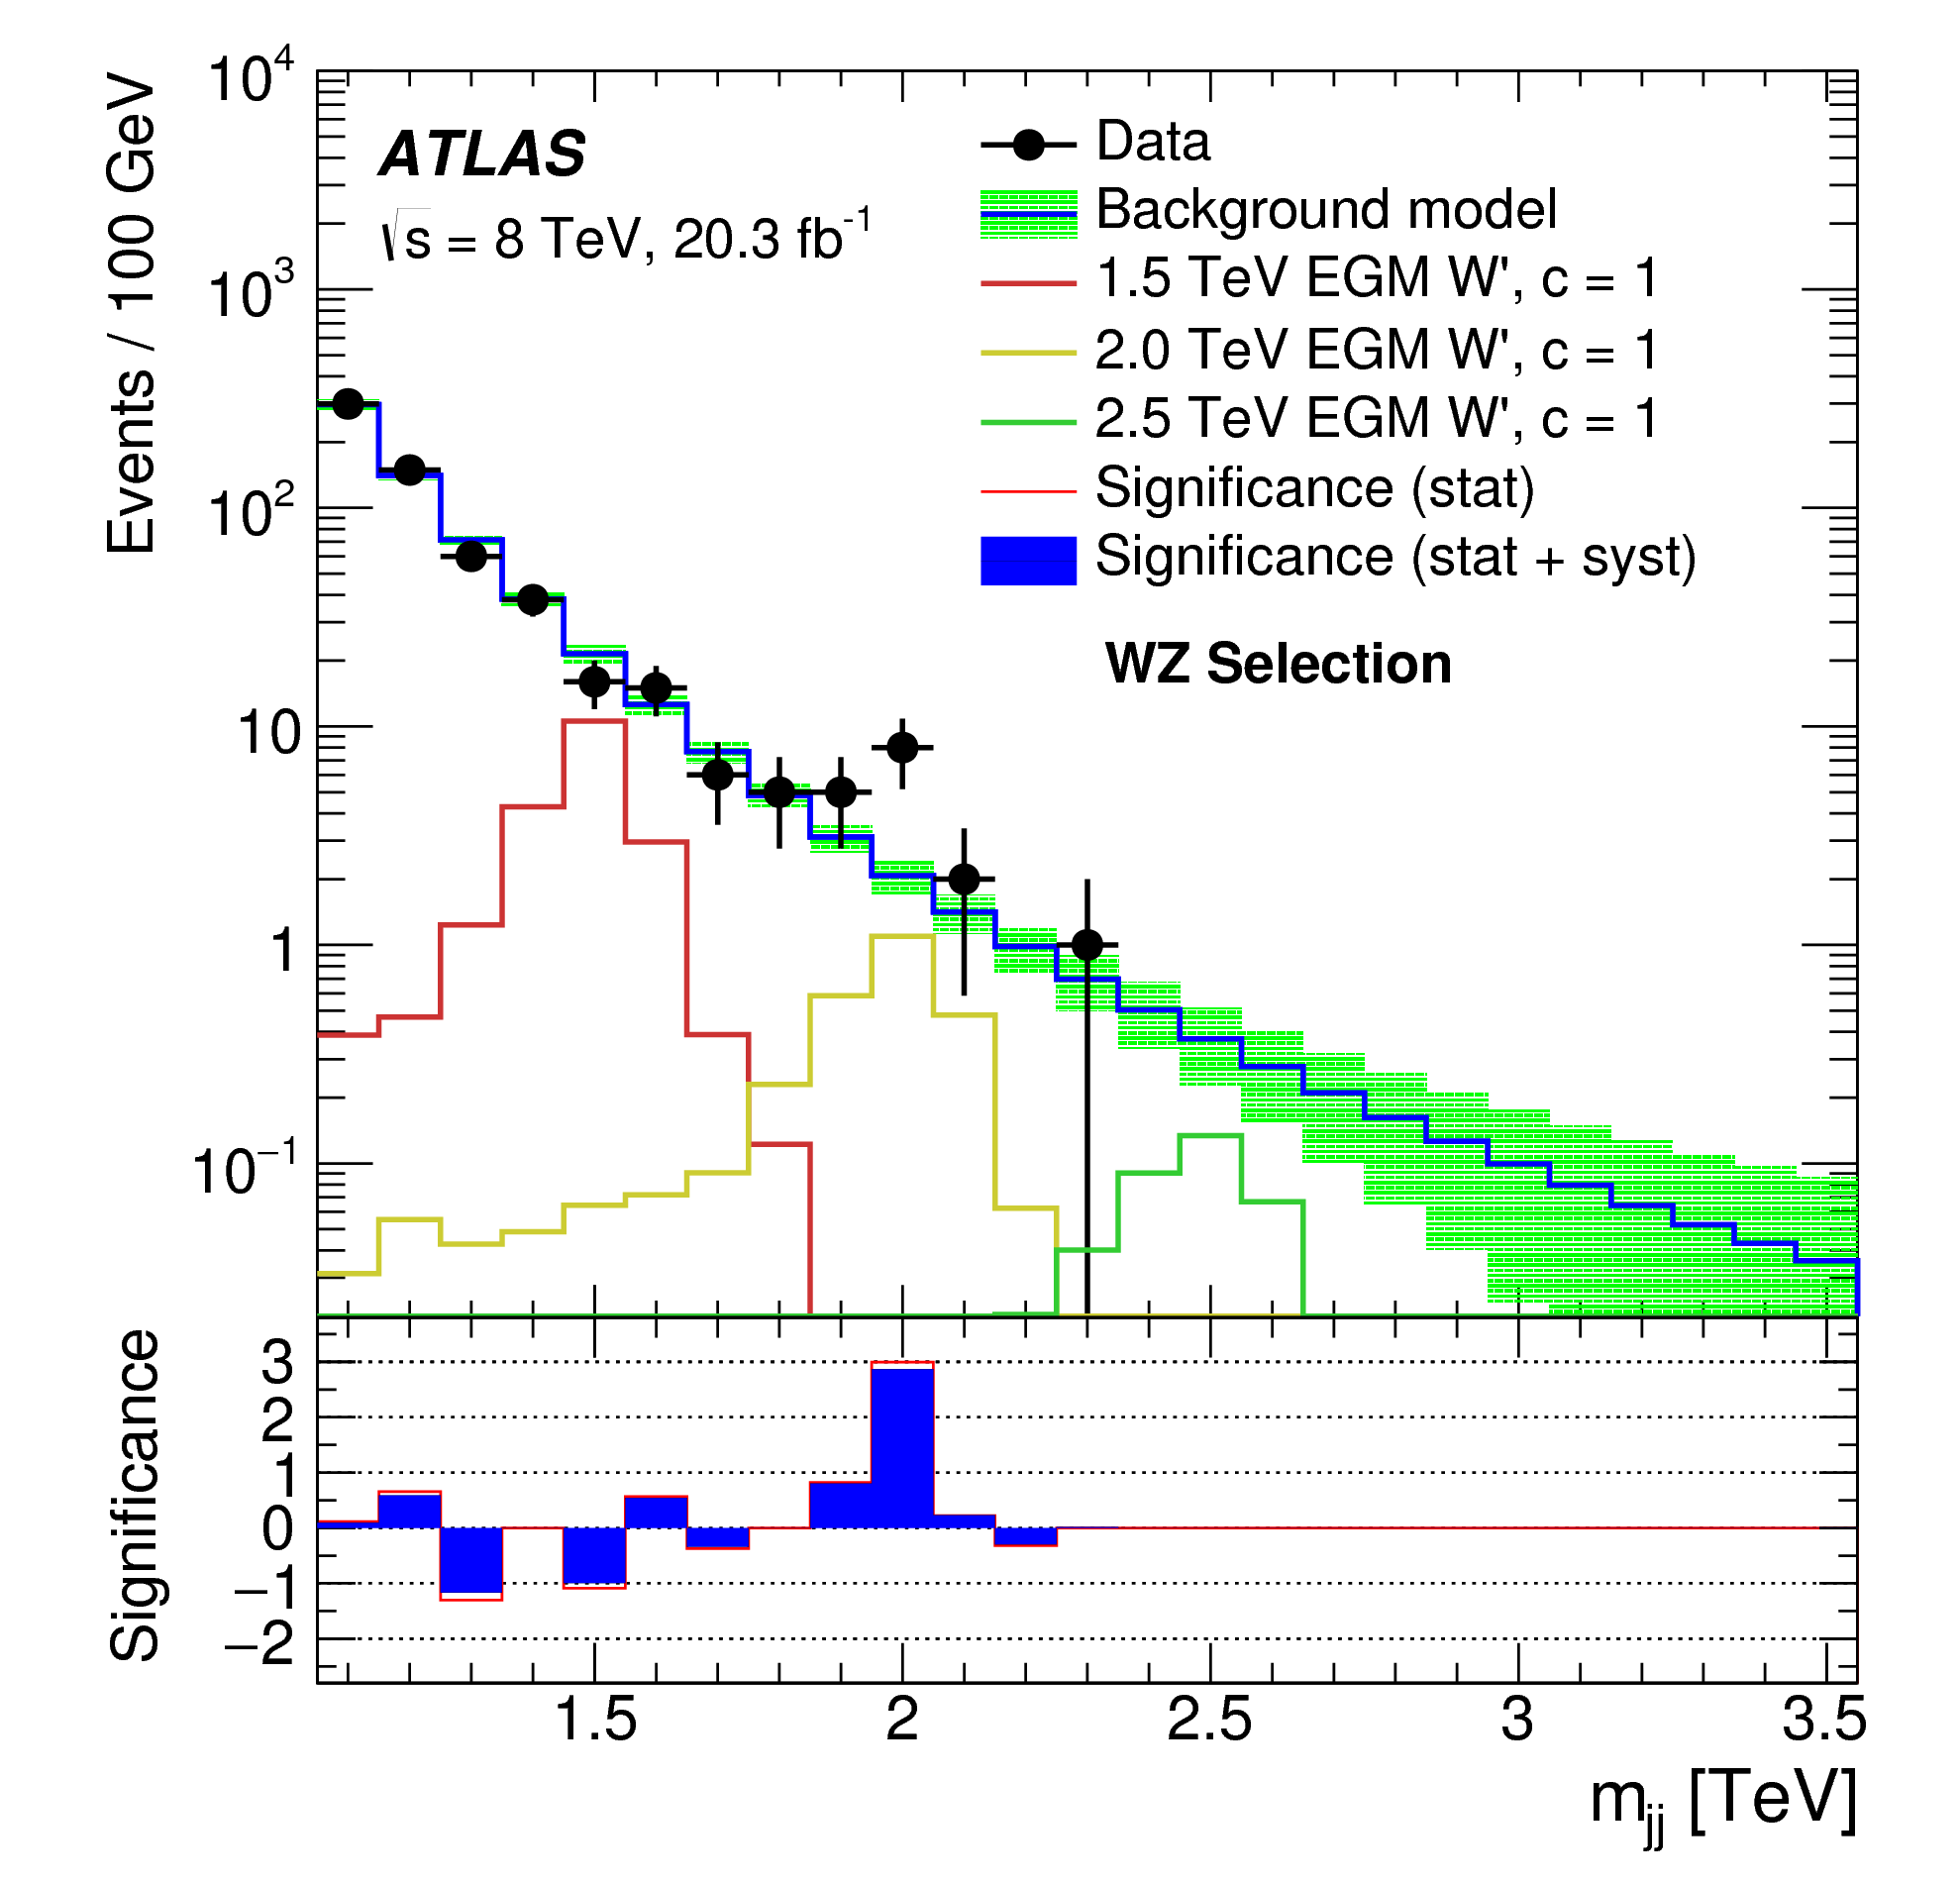
\includegraphics[width=0.4\textwidth]{figures/analysis/search1/misc/atlas_8tev.png}
    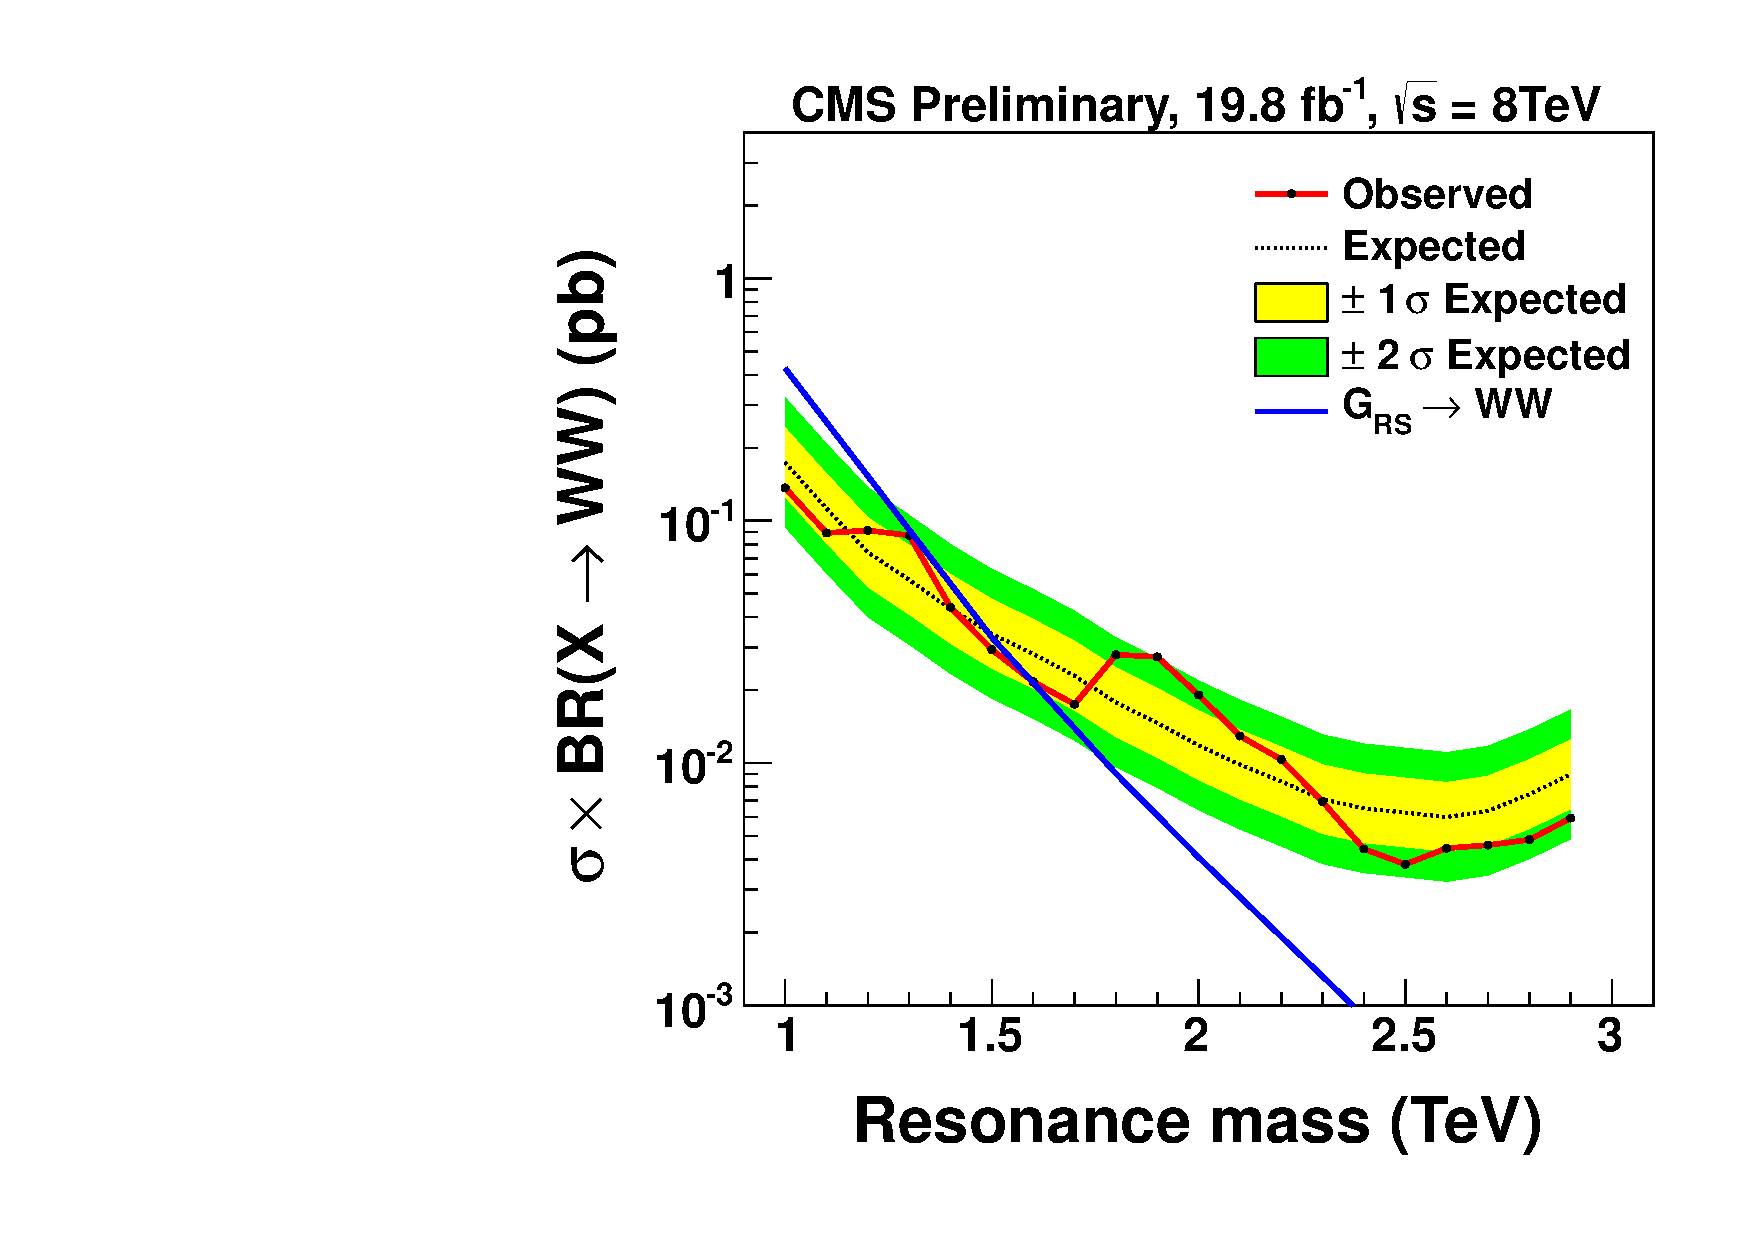
\includegraphics[width=0.4\textwidth]{figures/analysis/search1/misc/EXO-12-024_gWW.pdf}
    \caption{A "bump" corresponding to 3.4 $\sigma$ in the dijet invariant mass spectrum around 2 \TeV (left) observed by ATLAS when analyzing the full 8 \TeV dataset~\cite{Aad2015}, together with a similar excess (1.3 $\sigma$) observed in the corresponding CMS analysis~\cite{Khachatryan:1700394}.}
    \label{fig:searchI:8tev}
\end{figure}
The two measurements were found to be compatible, favoring a heavy resonance with a production cross section of around 5 femtobarn and a mass between 1.9 and 2.0 TeV decaying to either WW, WZ or ZZ~\cite{Dias:2015mhm}. Figure~\ref{fig:searchI:8tevcombo} shows the obtained p-value from the ATLAS (red) and CMS (blue) searches, as well as their combination (black). In addition to the observed excesses in the vector boson final states, another  $3 \sigma$ excess for a resonance with a mass of 1.8 \TeV had been observed in the search for heavy resonances decaying to a W and a Higgs boson~\cite{Khachatryan:2016yji} at 1.8 \TeV.
\begin{figure}[h!] 
    \centering
    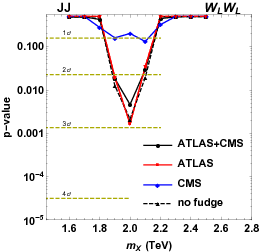
\includegraphics[width=0.25\textwidth]{figures/analysis/search1/misc/CMS_ATLAS_BulkWW_JJ_dijetfit_p.png}
    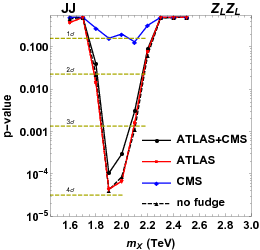
\includegraphics[width=0.25\textwidth]{figures/analysis/search1/misc/CMS_ATLAS_BulkZZ_JJ_dijetfit_p.png}
    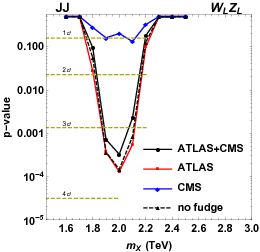
\includegraphics[width=0.25\textwidth]{figures/analysis/search1/misc/CMS_ATLAS_WZ_JJ_dijetfit_p.png}
    \caption{p-values as a function of resonance mass obtained with an emulation of the ATLAS (red) and CMS (blue) searches as well as the combination of the two (black). Here for a \PW\PW (left), \PW\PZ (middle) and \PZ\PZ (right) hypothesis~\cite{Dias:2015mhm}.}
    \label{fig:searchI:8tevcombo}
\end{figure}
The combination of the excesses and the timing of the ATLAS paper, naturally led to some excitement, and in the coming weeks, the arXiv was flooded with theory papers attempting an explanation of the deviations.\newline
In addition, one of the main benefits of increasing the LHC center-of-mass energy from 8 to 13 \TeV was that the partonic luminosity would increase.
One could therefore expect the same number of signal events in the 20 \fbinv data set collected with a center-of-mass energy of 8 TeV, for a considerably smaller luminosity with a center-of-mass energy of 13 TeV. Figure~\ref{fig:searchI:8vs13reach} shows the system mass that can be probed with the expected 2015 integrated luminosity of 3 \fbinv collected with a center-of-mass energy of 13 TeV, as a function of the probeable mass with 20 \fbinv of 8 TeV data for different partonic channels of qq, qg, and gg. For example, a 2 \TeV mass resonance would be observable in both datasets.
% The probable 13 \TeV mass is defined by finding the system mass which results in the same number of expected events at 8 \TeV, if assuming cross sections scale with partonic luminosity and $1/m^2$. Three different partonic scattering channels are considered: qq, qg and gg. We see that, for instance for a resonance with a mass of 2000 \GeV, the reach at 13 \TeV is 2241(gg), 2091(gq), 1851(qq, one type) and 2046(qq, all types) \GeV.
\begin{figure}[h!] 
    \centering
    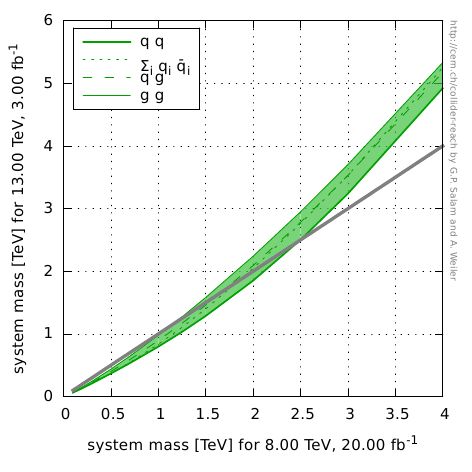
\includegraphics[width=0.50\textwidth]{figures/analysis/search1/misc/colliderReach.png}
    \caption{The system mass that can probed with 3 \fbinv of 13 \TeV data (y-axis) as a function of the probe-able system mass with 20 \fbinv of 8 \TeV data (x-axis) for different partonic channels (generated with~\cite{collreach}).}
    \label{fig:searchI:8vs13reach}
\end{figure}
We therefore expected that the small excess observed in the VV all-hadronic final state would be observable in the 2015 dataset if the signal was genuine.

\section{Analysis strategy}

When a resonance X with a mass above 1 TeV decays into a vector-boson pair, the bosons have a very high energy ($\tilde\PT=\mX/2=500 \GeV$, assuming X is produced at rest) is referred to as boosted. The decay products of a hadronically decaying boosted vector boson will therefore not appear as back-to-back in the lab frame but rather be collimated, as described in Section~\ref{sec:objreco:substructure}. This results in a final state with two high-pt, large-radius jets, such that the AK algorithm with an R=0.8 is expected to fully contain the two quarks coming from the vector boson decay. This is illustrated in Figure~\ref{fig:searchI:merged}.
\begin{figure}[h!] 
    \centering
    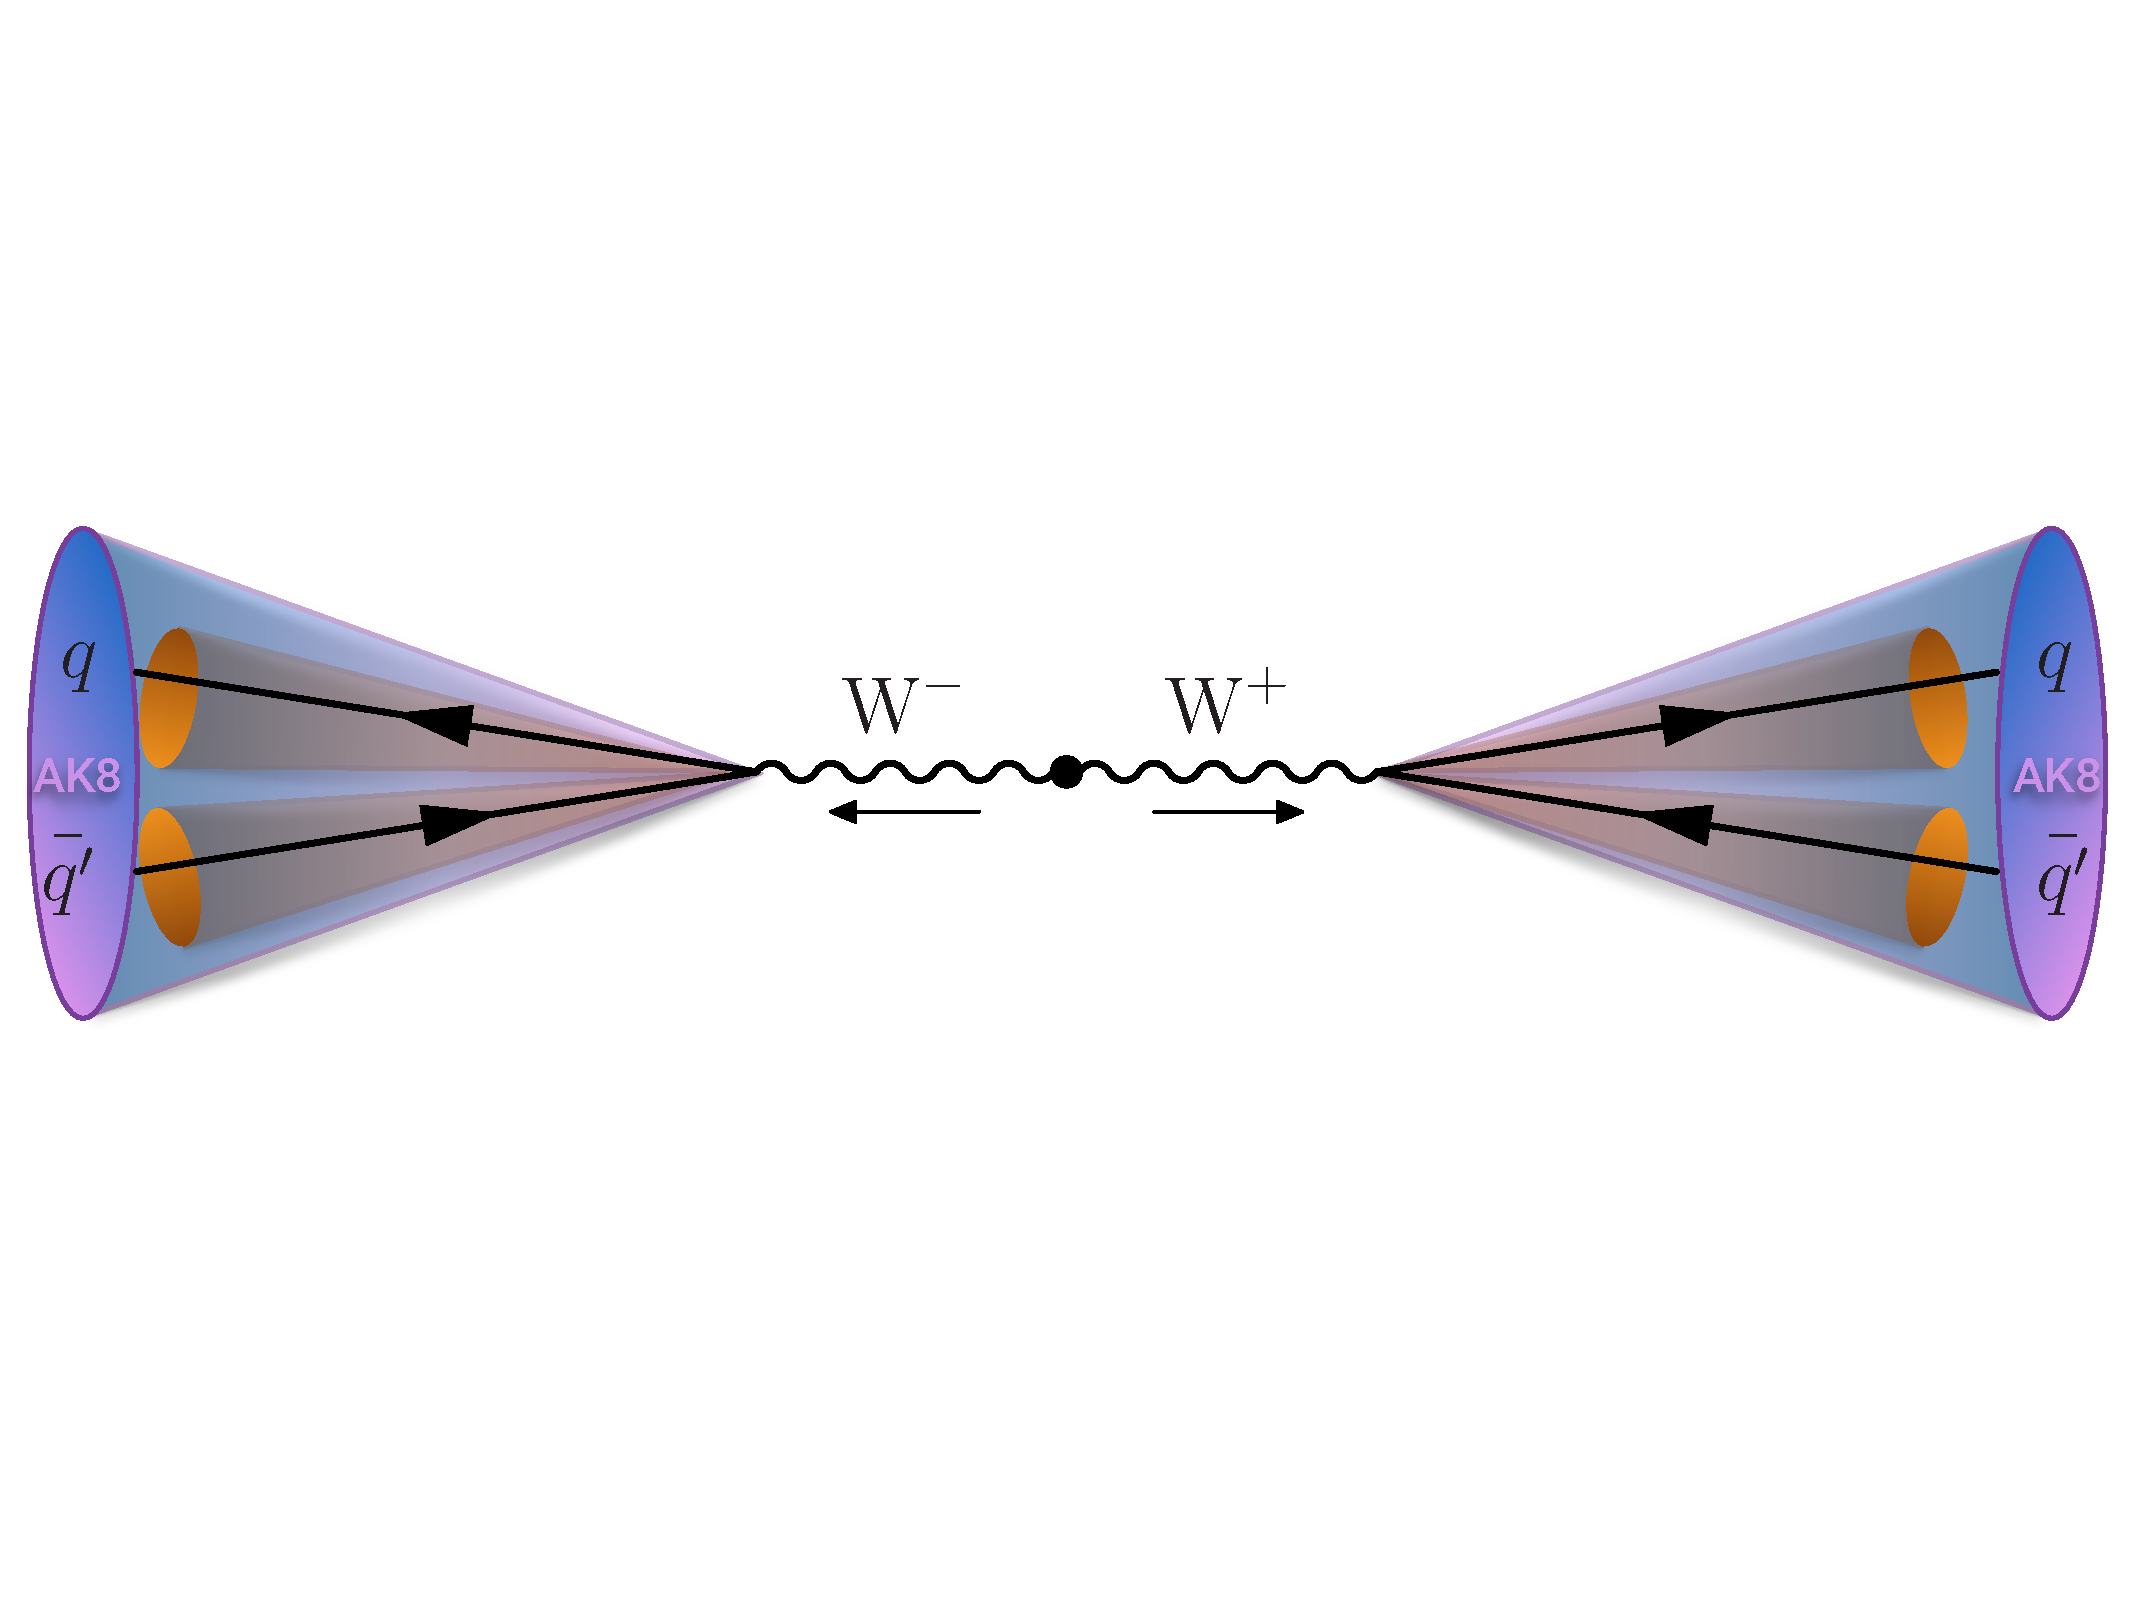
\includegraphics[width=0.70\textwidth]{figures/event_reconstruction/WWqqqq_merged_small.pdf}
    \caption{If a heavy ($>1 \TeV$) resonance decays into vector bosons, the transverse momentum of each boson will be large and its decay products are merged into one single large cone AK8 jet.}
    \label{fig:searchI:merged}
\end{figure}
The two jets are each expected to have a mass around the W or Z boson mass, and some intrinsic substructure stemming from their two-pronged decay. The invariant mass of the dijet system, \mjj, should be roughly equal to the resonance mass \mX. This dijet system is the final state under scrutiny and the dijet invariant mass is the parameter of interest. The final states of WW, ZZ, and WZ would produce similar final states. \par
The main background for such an analysis is QCD multijet events. As mentioned in Section~\ref{sec:objreco:substructure}, quark/gluon jets can obtain a high mass due to diffuse radiation and QCD processes have such a large cross section that the number of QCD jets with a mass compatible with the W mass can be large. In order to discriminate between the two, we take advantage of three properties. First, the groomed mass of signal and background jets should be very different. Second, signal jets should appear two-prong like, as opposed to quark/gluon jets, and third, the dijet invariant mass for the signal process should peak around the resonance mass while the QCD spectrum is predicted to be smoothly falling. Section~\ref{sec:searchI:bkg} explains this assumption in more detail. The strategy therefore consists of performing a smoothness test on \mjj of the observed data, a so-called "bump-hunt", by assuming that the signal will appear as a bump on top of a smooth distribution. This is illustrated in Figure~\ref{fig:searchI:bumphunt}.
\begin{figure}[h!] 
    \centering
    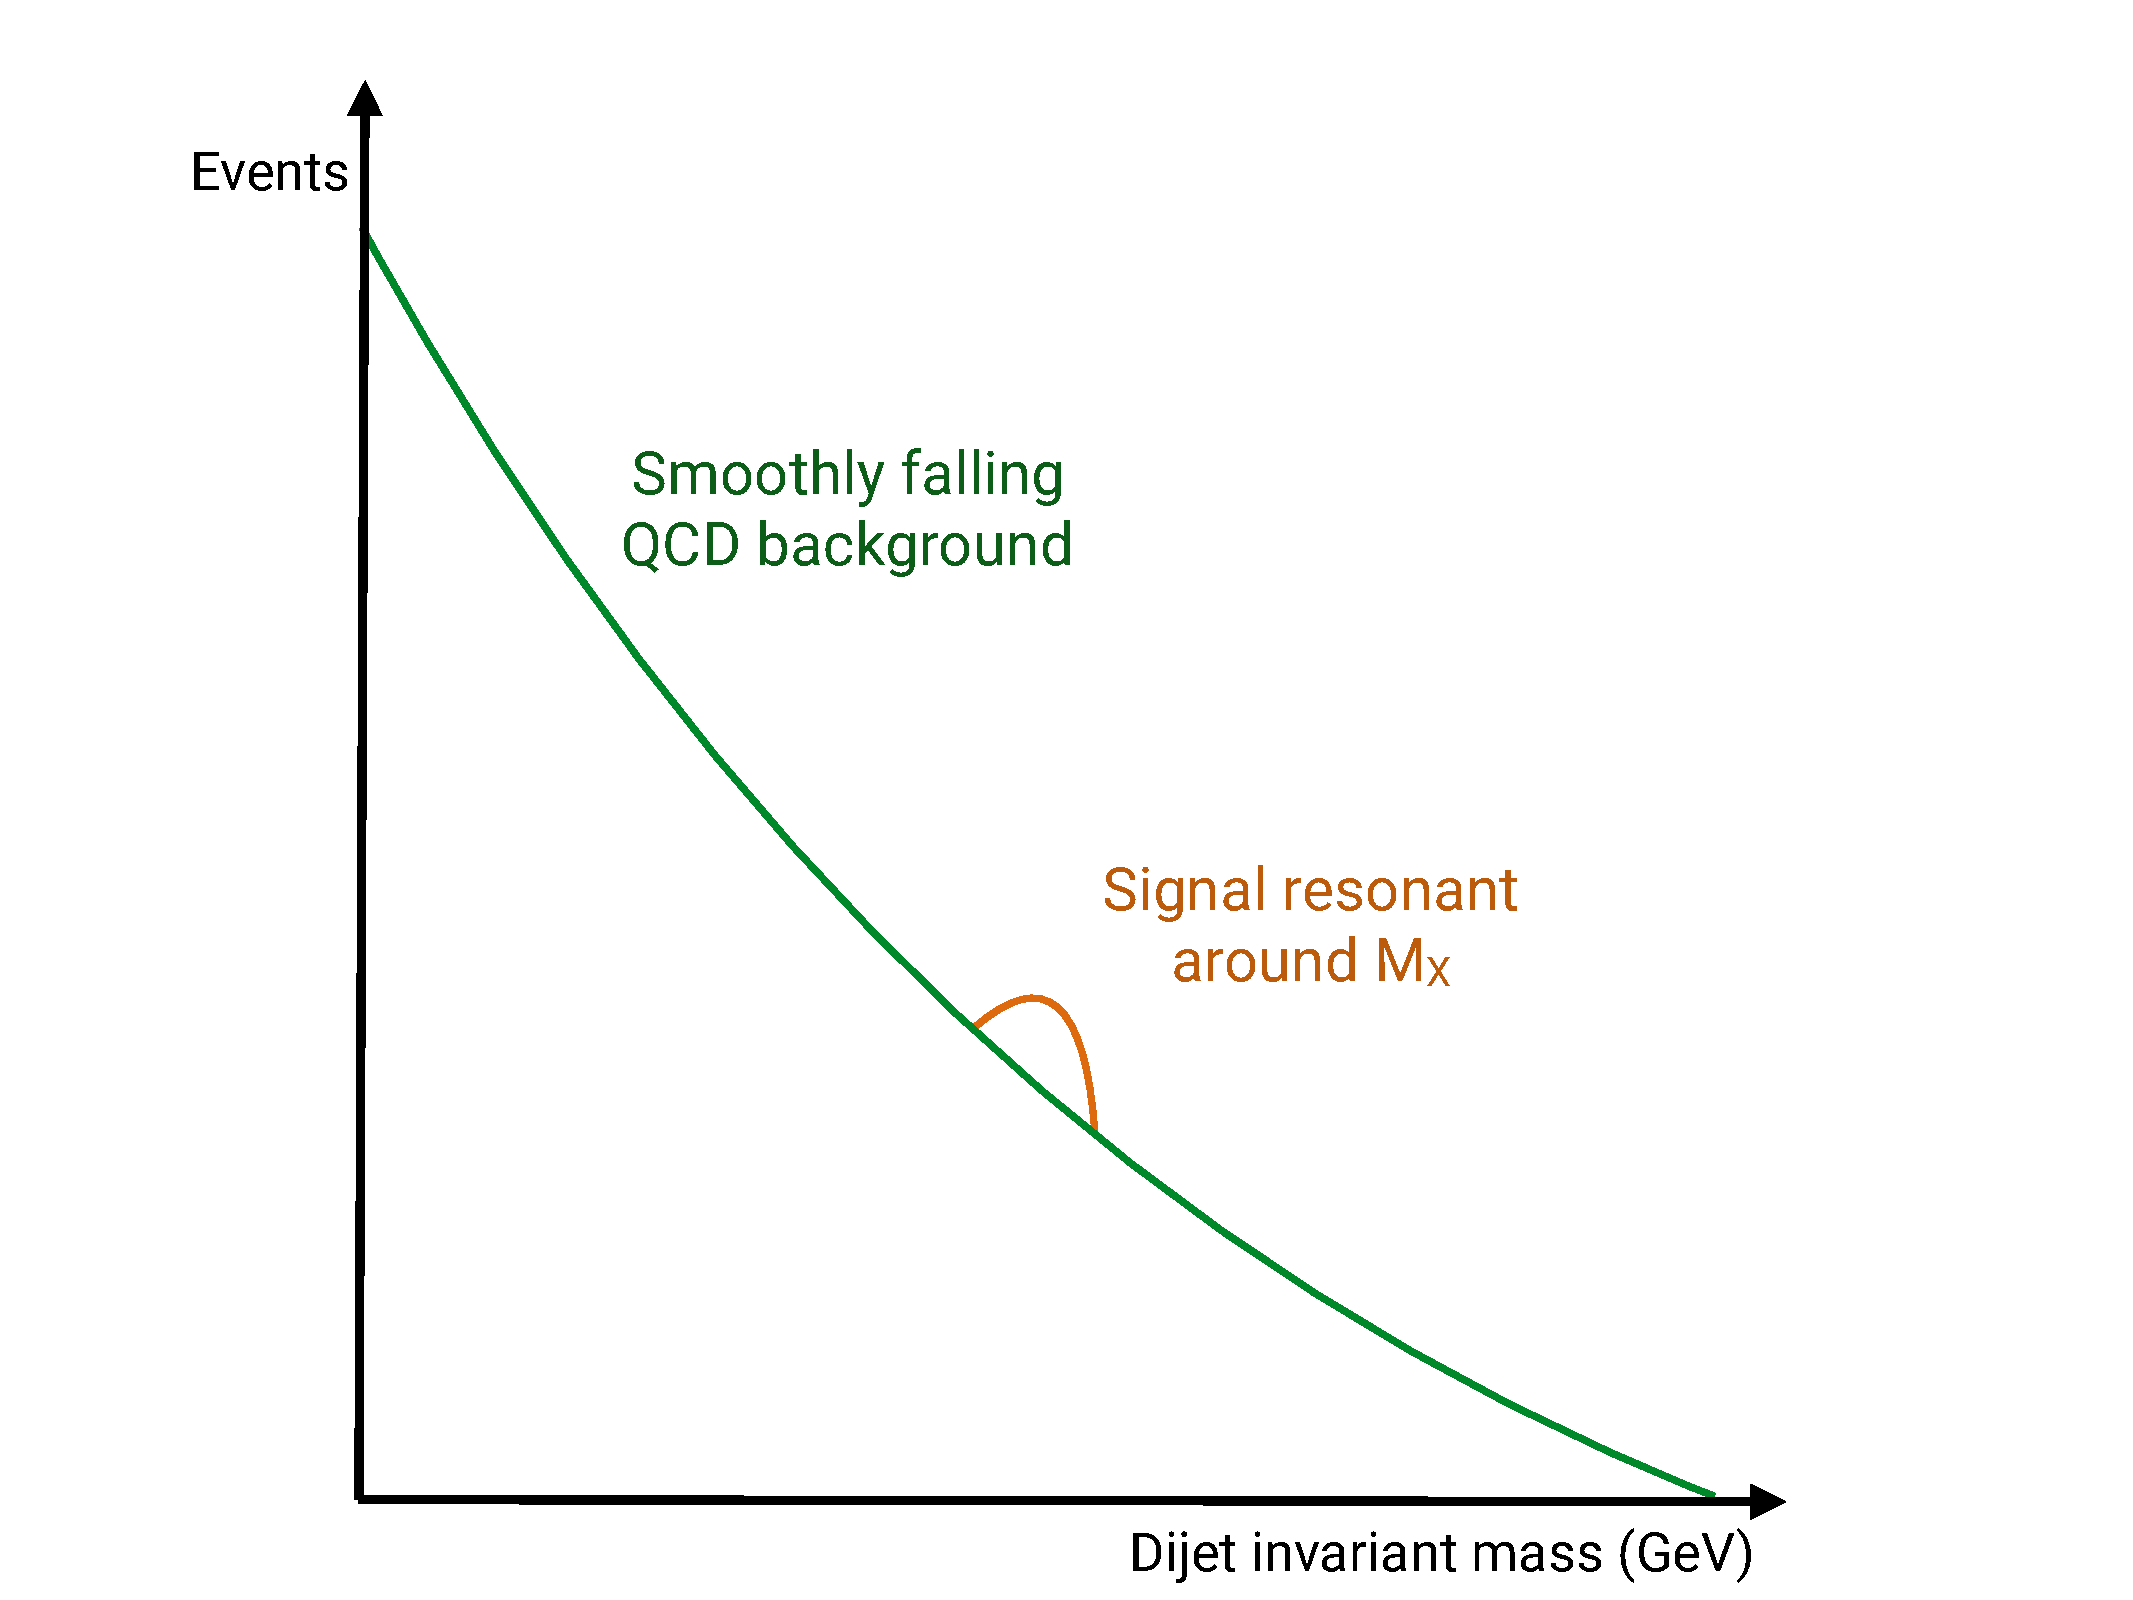
\includegraphics[width=0.49\textwidth]{figures/analysis/search1/misc/sigExtraction.pdf}
    \caption{The search strategy consists of looking for signal "bumps" in the dijet invariant mass on top of a smoothly falling QCD multijet background.}
    \label{fig:searchI:bumphunt}
\end{figure}
The benefit of such a method is that there is no need for a simulation of the background and the strategy is simple and robust. The disadvantage is that the analysis is intrinsically limited to regions where the dijet invariant mass spectrum is smooth and hence regions with discontinuities due to trigger turn-ons or kinematic selections must be avoided.

\section{Data and simulated samples}
\label{sec:searchI:samples}
The data analyzed in this search correspond to a total integrated luminosity of 2.7\fbinv collected at a center-of mass energy of 13 \TeV between June and December 2015. The instantaneous luminosity of the LHC during this run was around half of the design luminosity ($0.5 \times 10^{34} \percms$), with an average number of primary vertices per event of $<\mu>=13$. \par
The bulk graviton model (see Section~\ref{sec:theory:wed}) and the HVT model (\PWpr{} and \PZpr{}, see Section~\ref{sec:theory:hvt}) are used as benchmark signal processes. In these models, the vector gauge bosons are produced with a longitudinal polarization in more than 99\% of the cases, which leads to a 24\% higher acceptance per boson for reasons explained in Section~\ref{sec:objreco:pol}. For the HVT model, a scenario (model B) with $g_{\rm V}=3$, $c_{\rm H}=-0.976243$, and $c_{\rm F}=1.02433$ is chosen, where the heavy resonance predominantly couple to bosons and the coupling to fermions is suppressed. The bulk graviton samples were generated with $\ktilde = 0.5$. The resonance masses considered lie in the range 1.2 to 4 \TeV and are generated under the assumption of a natural width negligible with respect to the experimental resolution (narrow-width approximation). All signal samples are generated at leading order with \amcatnlo{} v2.2.2~\cite{Alwall:2014hca}. \par
Simulated samples of the production of QCD multijet events are generated to leading order using \PYTHIA version 8.205~\cite{Sjostrand:2007gs} with the CUETP8M1 tune~\cite{Khachatryan:2015pea} and are used to validate the analysis procedure.


\section{Event selection}

\subsection{Triggering}
\label{sec:searchI:trigger}
The first selection to be confronted in any analysis is the trigger selection. Due to an overwhelming QCD background in all-hadronic final states, the threshold for fully-hadronic triggers is very large in order to keep the trigger rate low (preferably around 10-30 Hz). In this analysis, we therefore decided to take advantage of triggers that place requirements on the jet's groomed mass in addition to the "standard" jet triggers based on the scalar sum of jet transverse energy \HT. These "boosted" triggers were never before tested in data, and this analysis was the first published result taking advantage of grooming at the trigger level in CMS. The following \HT-based High Level Triggers (HLT), referred to as inclusive triggers in the following, are used:
\begin{itemize}
\item \texttt{HLT\_PFHT650\_WideJetMJJ900DEtaJJ1p5},
\item \texttt{HLT\_PFHT650\_WideJetMJJ950DEtaJJ1p5}, and
\item \texttt{HLT\_PFHT800}.
\end{itemize}
Here, \emph{PFHT650} refers to a total \HT of at least 650 GeV. \emph{WideJet} means jets reconstructed with the \emph{wide jet algorithm}~\cite{2011123}, an algorithm inspired by jet grooming intended to reduce sensitivity to gluon radiation. The two AK R=0.4 jets with the largest \PT in the event are used as seeds. Geometrically close jets are then combined into the closest jet seed if they are within $\Delta R = \sqrt{(\Delta \eta)^2+\Delta \phi)^2}$, and these two jets form a dijet system used for further selections. \emph{MJJ900} refers to a wide-jet dijet mass of at least 900 GeV, and \emph{DetaJJ1p5} means there is an additional cut on the $|\Delta \eta|$ between the two wide jets for reasons that will be explained below. In addition, two triggers based on jet grooming are used. These require a trimmed jet mass (see Section 3.5.1) of 30 and 50 GeV, yielding the triggers:
\begin{itemize}
\item \texttt{HLT\_AK8PFJet360\_TrimMass30} and
\item \texttt{HLT\_AK8PFHT700\_TrimR0p1PT0p03Mass50}.
\end{itemize}
The tuneable parameters for the trimming algorithm at HLT are $r_{sub}=0.2$ and $p_{T,frac}=0.03$. The \texttt{HLT\_AK8PFJet360\_TrimMass30} trigger is seeded by single-object Level 1 triggers with jet $p_T$ thresholds of 176 or 200 GeV (\texttt{L1\_SingleJet176} or \texttt{L1\_SingleJet200}), and the remaining triggers require an online \HT{}$>$150 or 175 GeV (\texttt{L1\_HTT150} or \texttt{L1\_HTT175}).\par
In order to avoid any kinks in the dijet invariant mass spectrum due to the presence of a trigger turn-on, we determine the dijet invariant mass at which the analysis triggers are fully efficient ($>99\%$), and only consider signal events above this value. In order to estimate the trigger efficiency, we use a trigger with a lower \HT threshold, \texttt{HLT\_PFHT650}, as a reference trigger. This trigger has a prescale of 40, meaning events are only recorded one out of 40 times. It is seeded by L1 \HT triggers with thresholds of 150 or 175 GeV. We then define the efficiency as
\begin{equation*}
\textrm{Efficiency} = \frac{N_{trigger+ref}}{N_{ref}}  
\end{equation*}
where $N_{trigger+ref}$ corresponds to the number of events passing the trigger under study as well as the reference trigger, and $N_{ref}$ corresponds to the number of events passing the reference trigger. Figure~\ref{fig:searchI:trigger-fits} shows the trigger turn-on curves as a function of dijet invariant mass for jets where one of the jets is required to have a pruned mass larger than 65 GeV (in other words, compatible with a W jet). A sharp turn-on for the inclusive triggers (top left) is observed, reaching the 100\% efficiency plateau for dijet masses of around 1.0--1.1 TeV. The grooming triggers, however, turn on more slowly and are not fully efficient until dijet invariant masses reach around 1.2 TeV (top right). The real power of the grooming triggers become clear when considering them in addition to the \HT-based triggers. The bottom plot in Figure~\ref{fig:searchI:trigger-fits} compares the trigger turn-on curves as a function of dijet invariant mass for jets passing one of the three inclusive triggers only, one of the grooming triggers only, and when combining all of them. Here, one can see that the 99\% efficiency threshold is lowered by 75 \GeV when including the substructure triggers, once substructure is required at analysis level. This combination of triggers allowed the analysis to consider dijet invariant masses as low as 1 TeV.
\begin{figure}[h!]
\centering
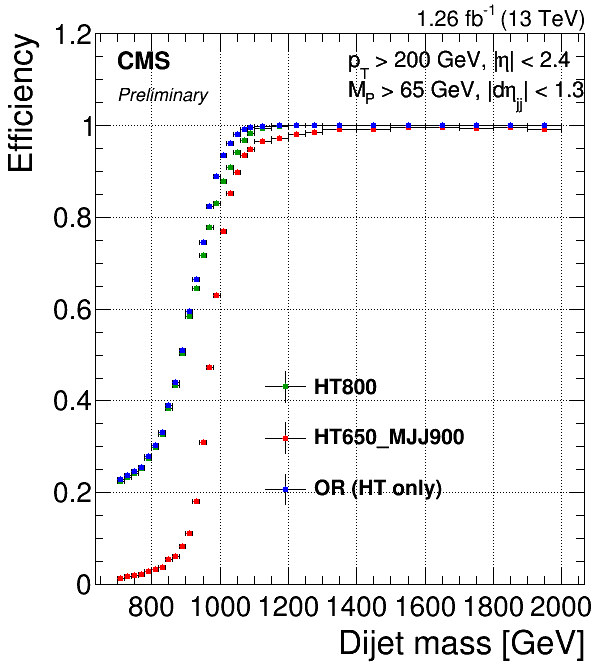
\includegraphics[width=0.4\textwidth]{figures/analysis/search1/AN-15-211//triggereffMjj-HT.png}
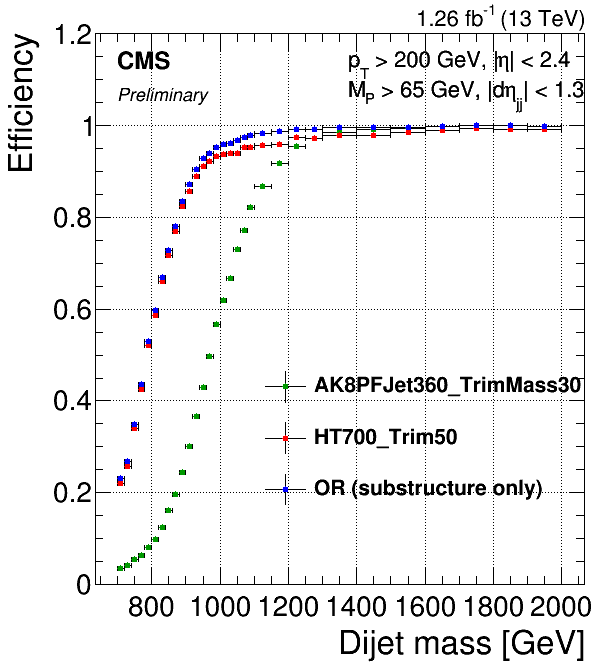
\includegraphics[width=0.4\textwidth]{figures/analysis/search1/AN-15-211//triggereffMjj-SUBST.png}\\
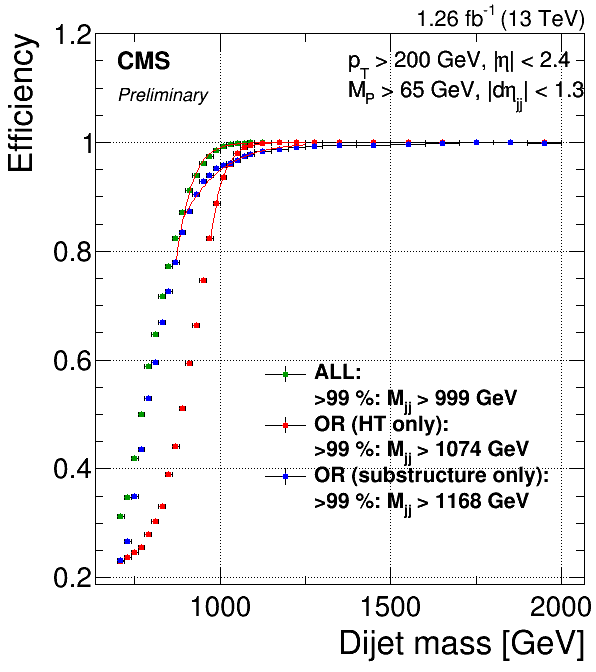
\includegraphics[width=0.4\textwidth]{figures/analysis/search1/AN-15-211/triggereffMjj-ALL.png}
\caption{Top: Efficiency for the inclusive triggers (top left) and the grooming triggers (top right) as a function of dijet invariant mass for jet pairs where one jet has a pruned mass larger than 65 GeV. Bottom: Comparison of trigger efficiencies for jets passing one of the HT-triggers only (red), for jets passing one of the grooming-triggers only (blue) and for jets passing one of the HT-triggers or one of the grooming triggers (green). Here as a function of dijet invariant mass for all jet pairs passing loose selections and where one jet has a pruned mass larger than 65 GeV. The 99\% efficiency threshold is lowered by 75 \GeV when including substructure taggers.}
\label{fig:searchI:trigger-fits}
\end{figure}
As a measure of the performance of the grooming triggers, we have in addition looked at the trigger efficiencies as a function of the offline groomed mass (using the pruned and softdrop algorithms described in Sections~\ref{sec:objreco:pruning} and ~\ref{sec:objreco:softdrop}), for the grooming trigger with the lowest mass threshold (30 \GeV). This is shown in Figure~\ref{fig:searchI:grooming-mj-trigger}, where an additional cut on the jet transverse momentum of one of the jets of 600 GeV is required and no other mass cut is applied. The trigger plateau is reached for offline groomed-jet masses around 50 GeV. 
\begin{figure}[h!]
\centering
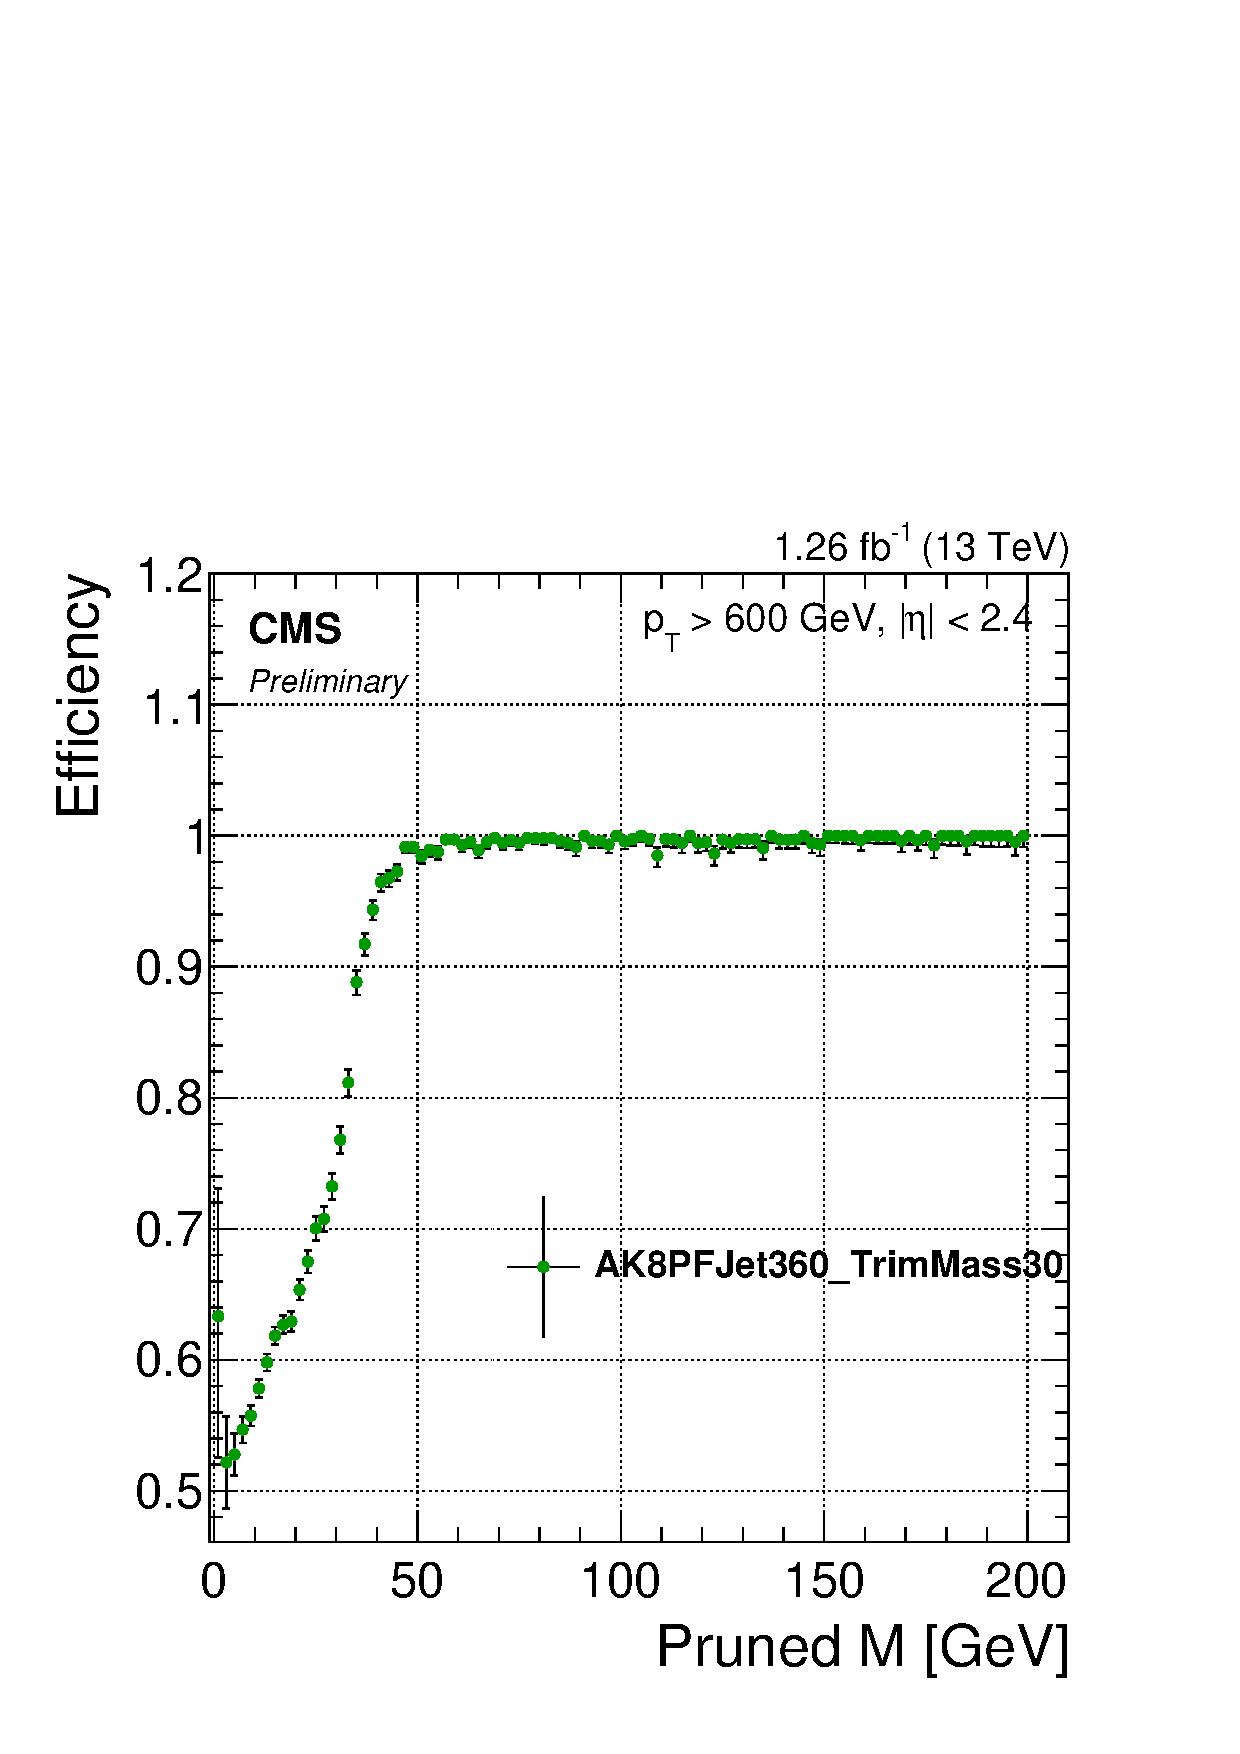
\includegraphics[width=0.4\textwidth]{figures/analysis/search1/AN-15-211//triggereff-prunedmass600.pdf}
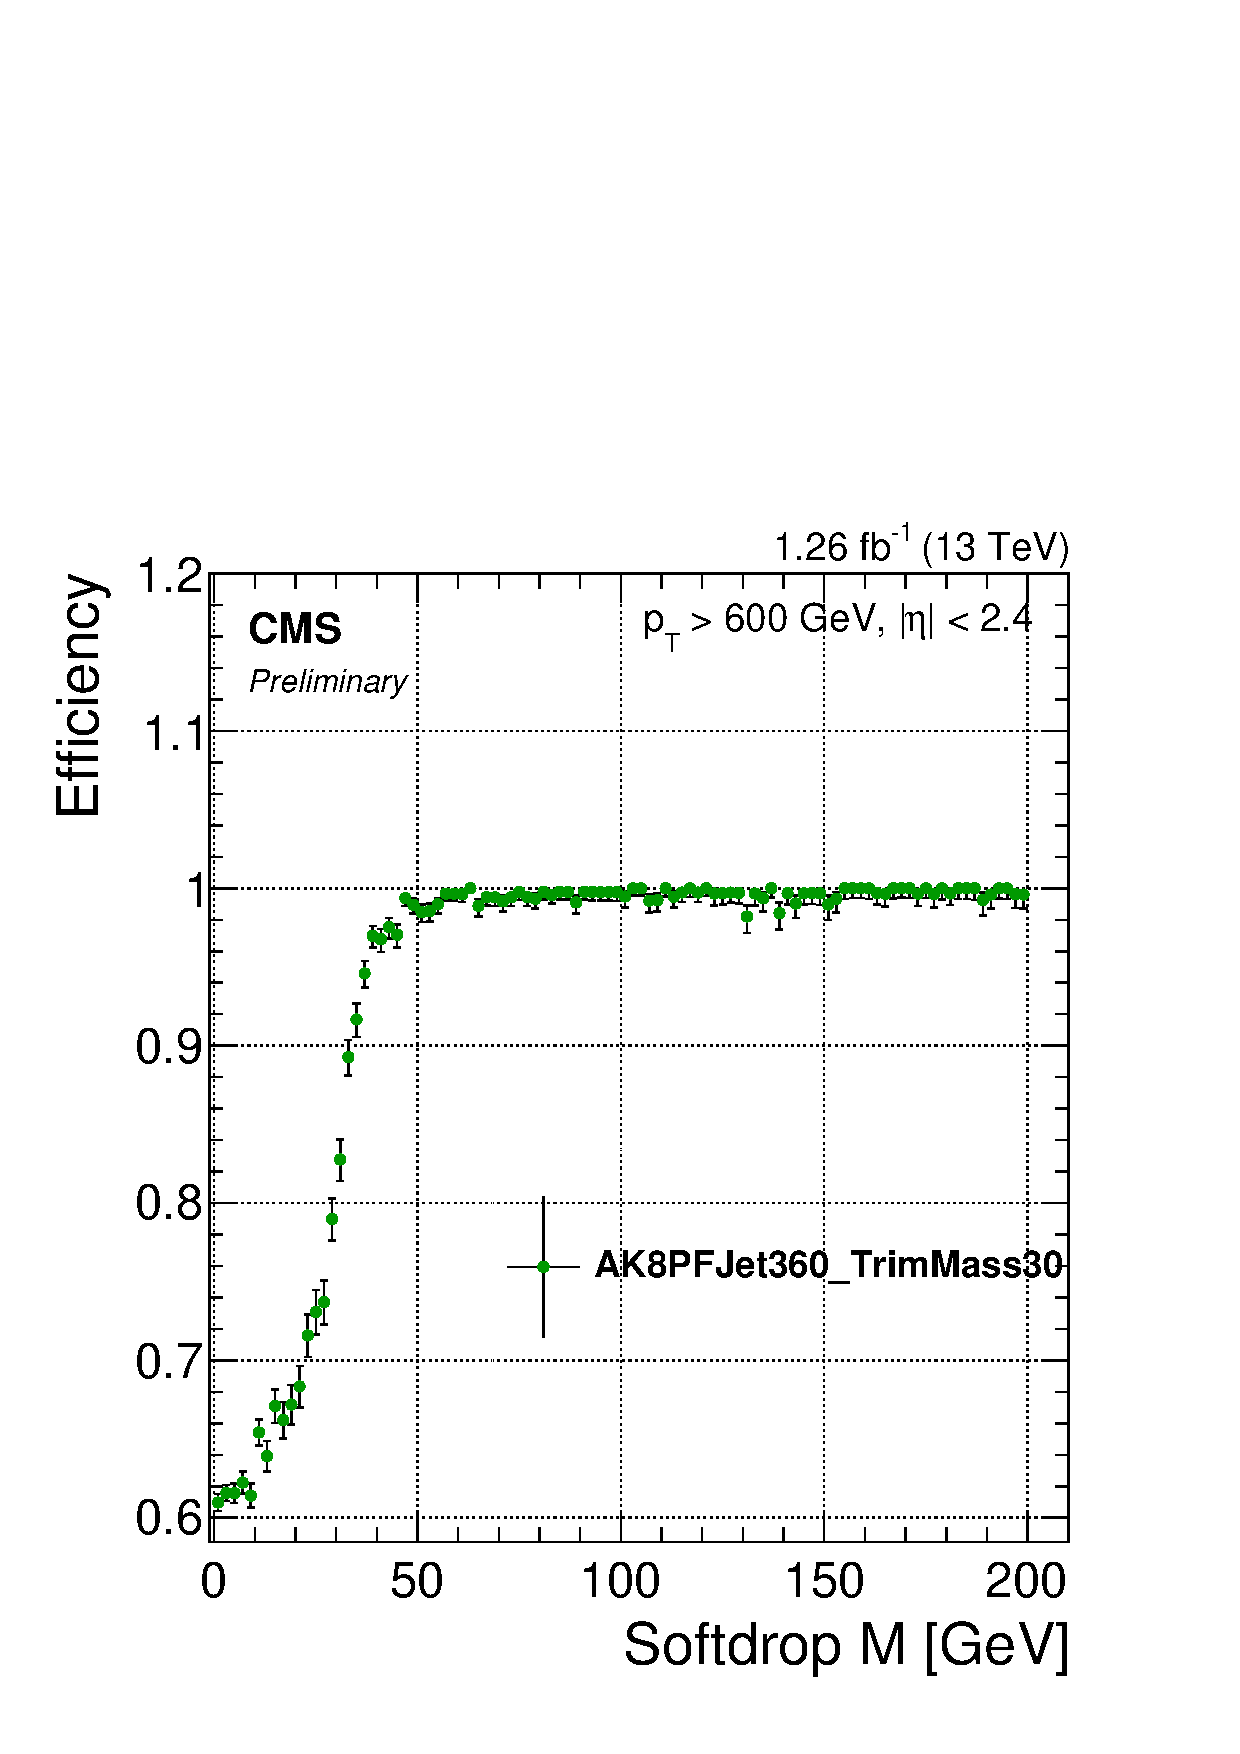
\includegraphics[width=0.4\textwidth]{figures/analysis/search1/AN-15-211//triggereff-sdmass.pdf}
\caption{Efficiency for the lowest threshold grooming trigger as a function of pruned-jet (left) and softdrop-jet (right) mass for jets with $\PT > \unit{600}{\GeV}$.}
\label{fig:searchI:grooming-mj-trigger}
\end{figure}

\subsection{Preselection} 
\label{sec:searchI:preselection}
After trigger selections, and the corresponding requirement of a dijet invariant mass above 1 \TeV to ensure a smoothy falling background, we begin the process of maximizing the signal significance while keeping the background low. This is done by optimizing the selection requirements on the jets. The jets used in this analysis are clustered with the anti-\kt{} jet clustering algorithm with a clustering parameter of $R=0.8$ (see Section ~\ref{sec:objreco:jets}) to allow containment of the full vector-boson decay products. Since a minimum transverse momentum of 200 \GeV is required for the decay products of a W/Z to be fully contained within an R=0.8 jet, events are further selected by requiring at least two jets with $\PT > \unit{200}{\GeV}$. These are in addition required to be central, with an $|\eta| < 2.4$. The two highest \PT jets in the event passing these criteria are selected as potential vector boson candidates. As our main background is QCD multijet events, we further take advantage of the fact that the angular distribution between these, mainly t-channel, processes are very different from the s-channel signal processes under study. The crossection for QCD t-channel processes as a function of the opening angle with respect to the beam axis ($\theta*$), exhibit a pole around $\cos \theta*=1$, meaning QCD t-channel jets are mostly produced in the forward direction, with an opening angle with respect to the beam axis close to zero. The signal jets on the other hand, produced through an s-channel process, are concentrated in the barrel region. We therefore require the jets to have a separation of $|\Delta\eta|<1.3$ in order to reduce the QCD multijets background. The distribution of $|\Delta\eta|$ between the two highest-\PT jets for QCD, as well as for different signal scenarios, is shown in Figure~\ref{fig:searchI:detaopt}.
\begin{figure}[h!]
\centering
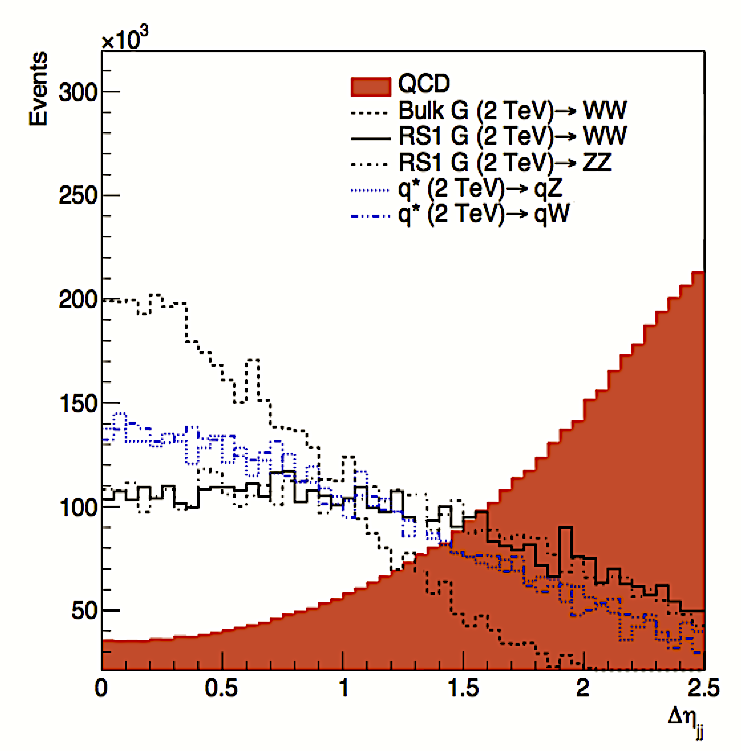
\includegraphics[width=0.4\textwidth]{figures/analysis/search1/misc/deta_opt.png}
\caption{ $|\Delta\eta|$  between the two highest-\PT jets for QCD jets and jets stemming from different signal scenarios.}
\label{fig:searchI:detaopt}
\end{figure}
A cut of $|\Delta \eta|_{jj}<1.3$ removes the t-channel pole at $\cos \theta* = 1$ and is in addition found to yield the highest signal sensitivity. In addition to these requirements on the jets themselves, a veto on jets overlapping with leptons is applied. Here the overlap $\Delta R(\text{jet},\text{lepton})$ between the jet candidate and a lepton is required to be larger than 0.8. Leptons used for this veto are required to pass the identification requirements described in Section~\ref{sec:objreco:electrons} and~\ref{sec:objreco:muons}, have a transverse momentum larger than 35 (30) GeV, and a pseudorapidity smaller than 2.5 (2.4) in the case of electrons (muons). The \PT, $\eta$, dijet invariant mass, and $|\Delta \eta|_{jj}$ distribution for the two leading jets in the event after the above preselections have been applied is shown in Figure~\ref{fig:kinematics-all}.
\begin{figure}[h!]
\centering
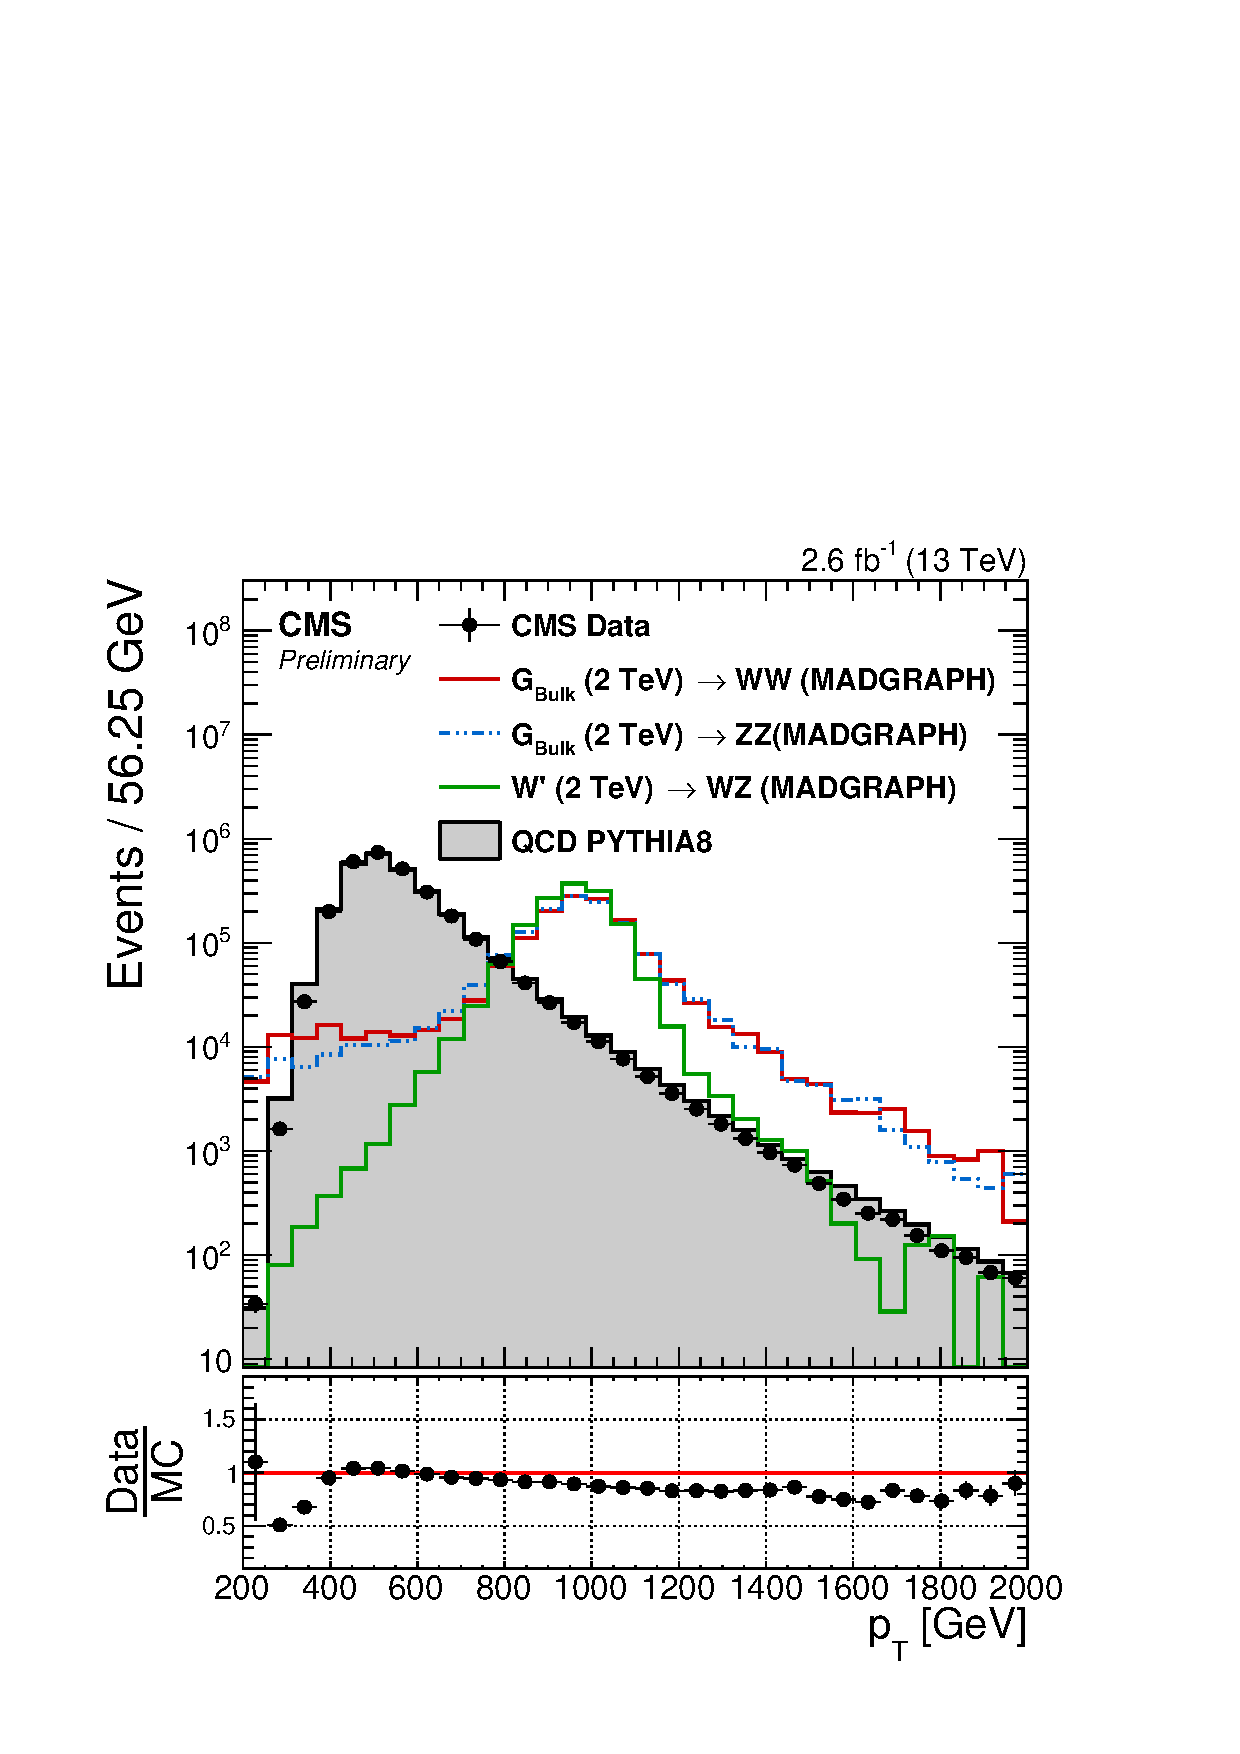
\includegraphics[width=0.4\textwidth]{figures/analysis/search1/AN-15-211/controlplots/silverjson/Pt_WSignal.pdf}
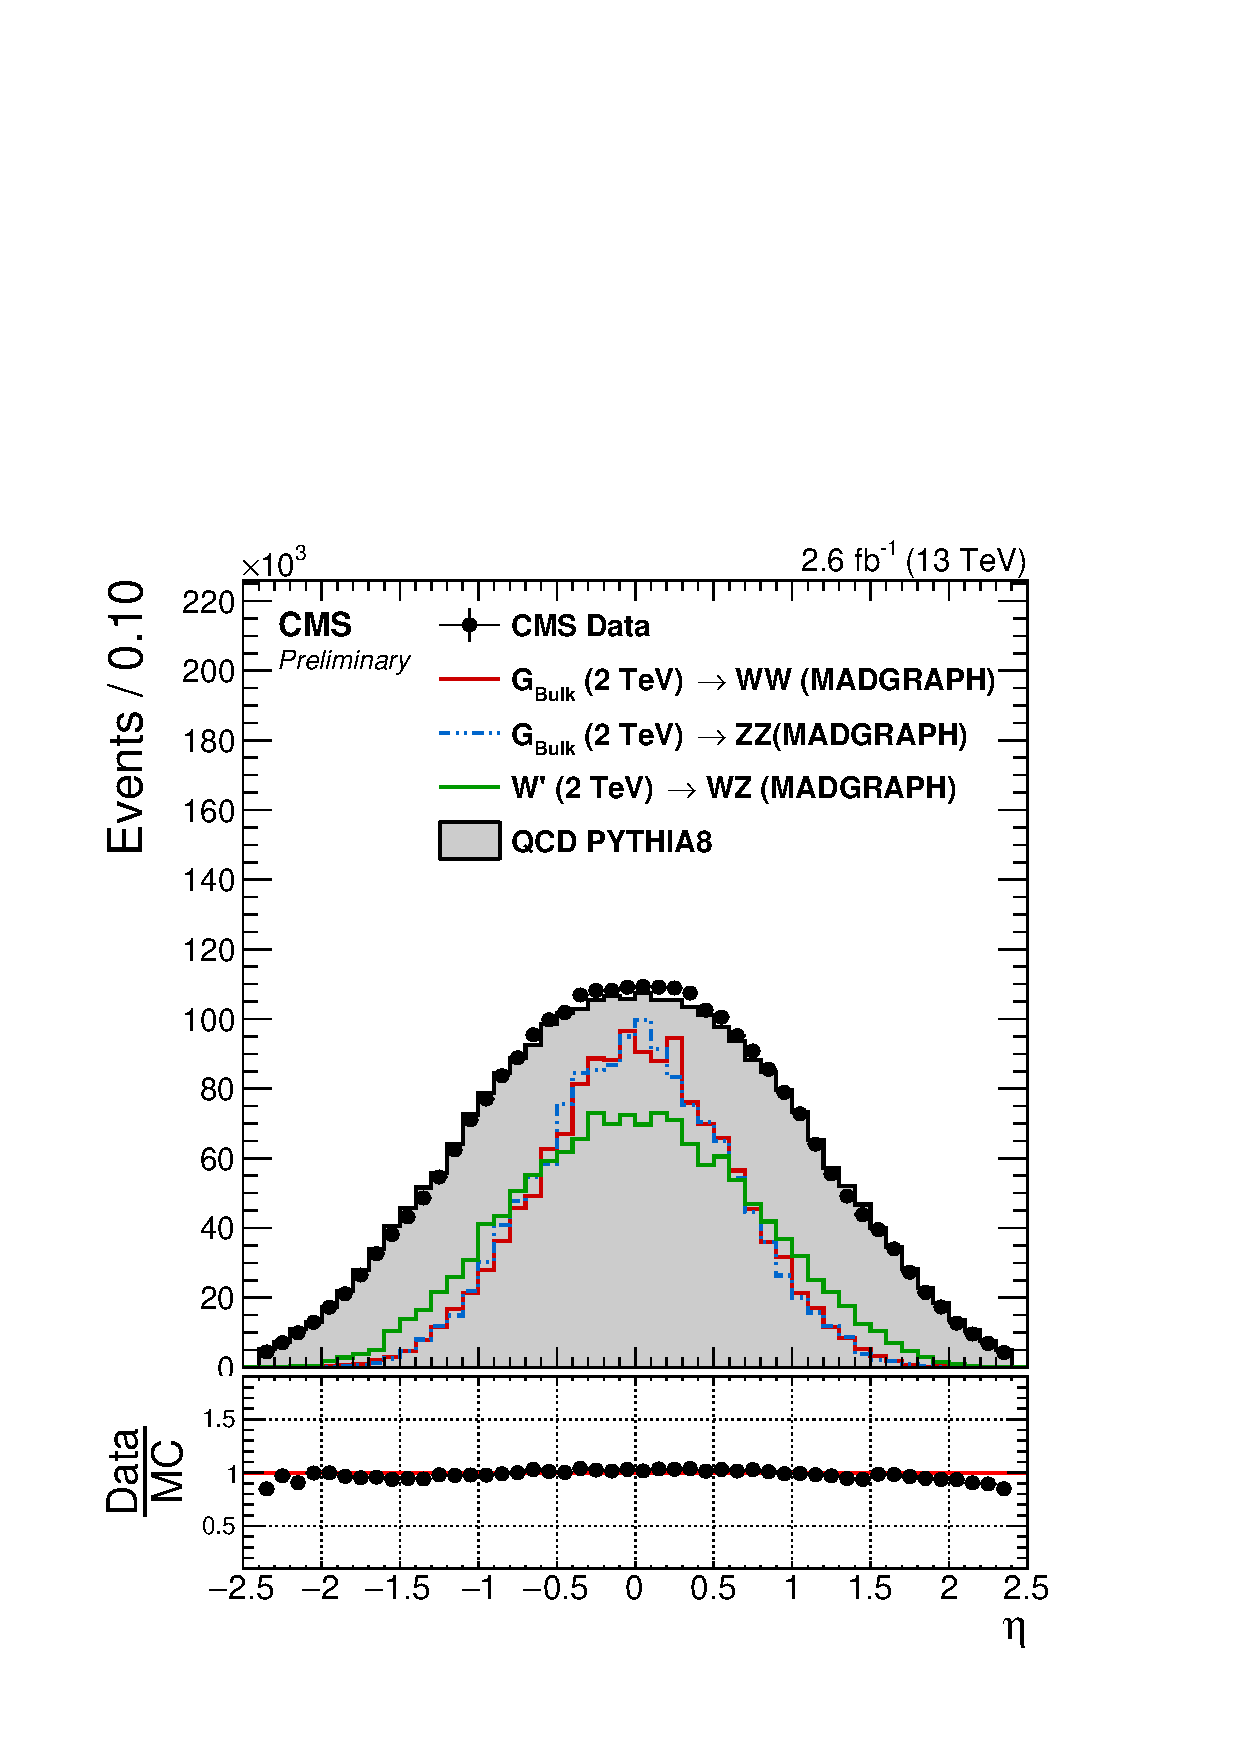
\includegraphics[width=0.4\textwidth]{figures/analysis/search1/AN-15-211/controlplots/silverjson/Eta_WSignal.pdf}\\
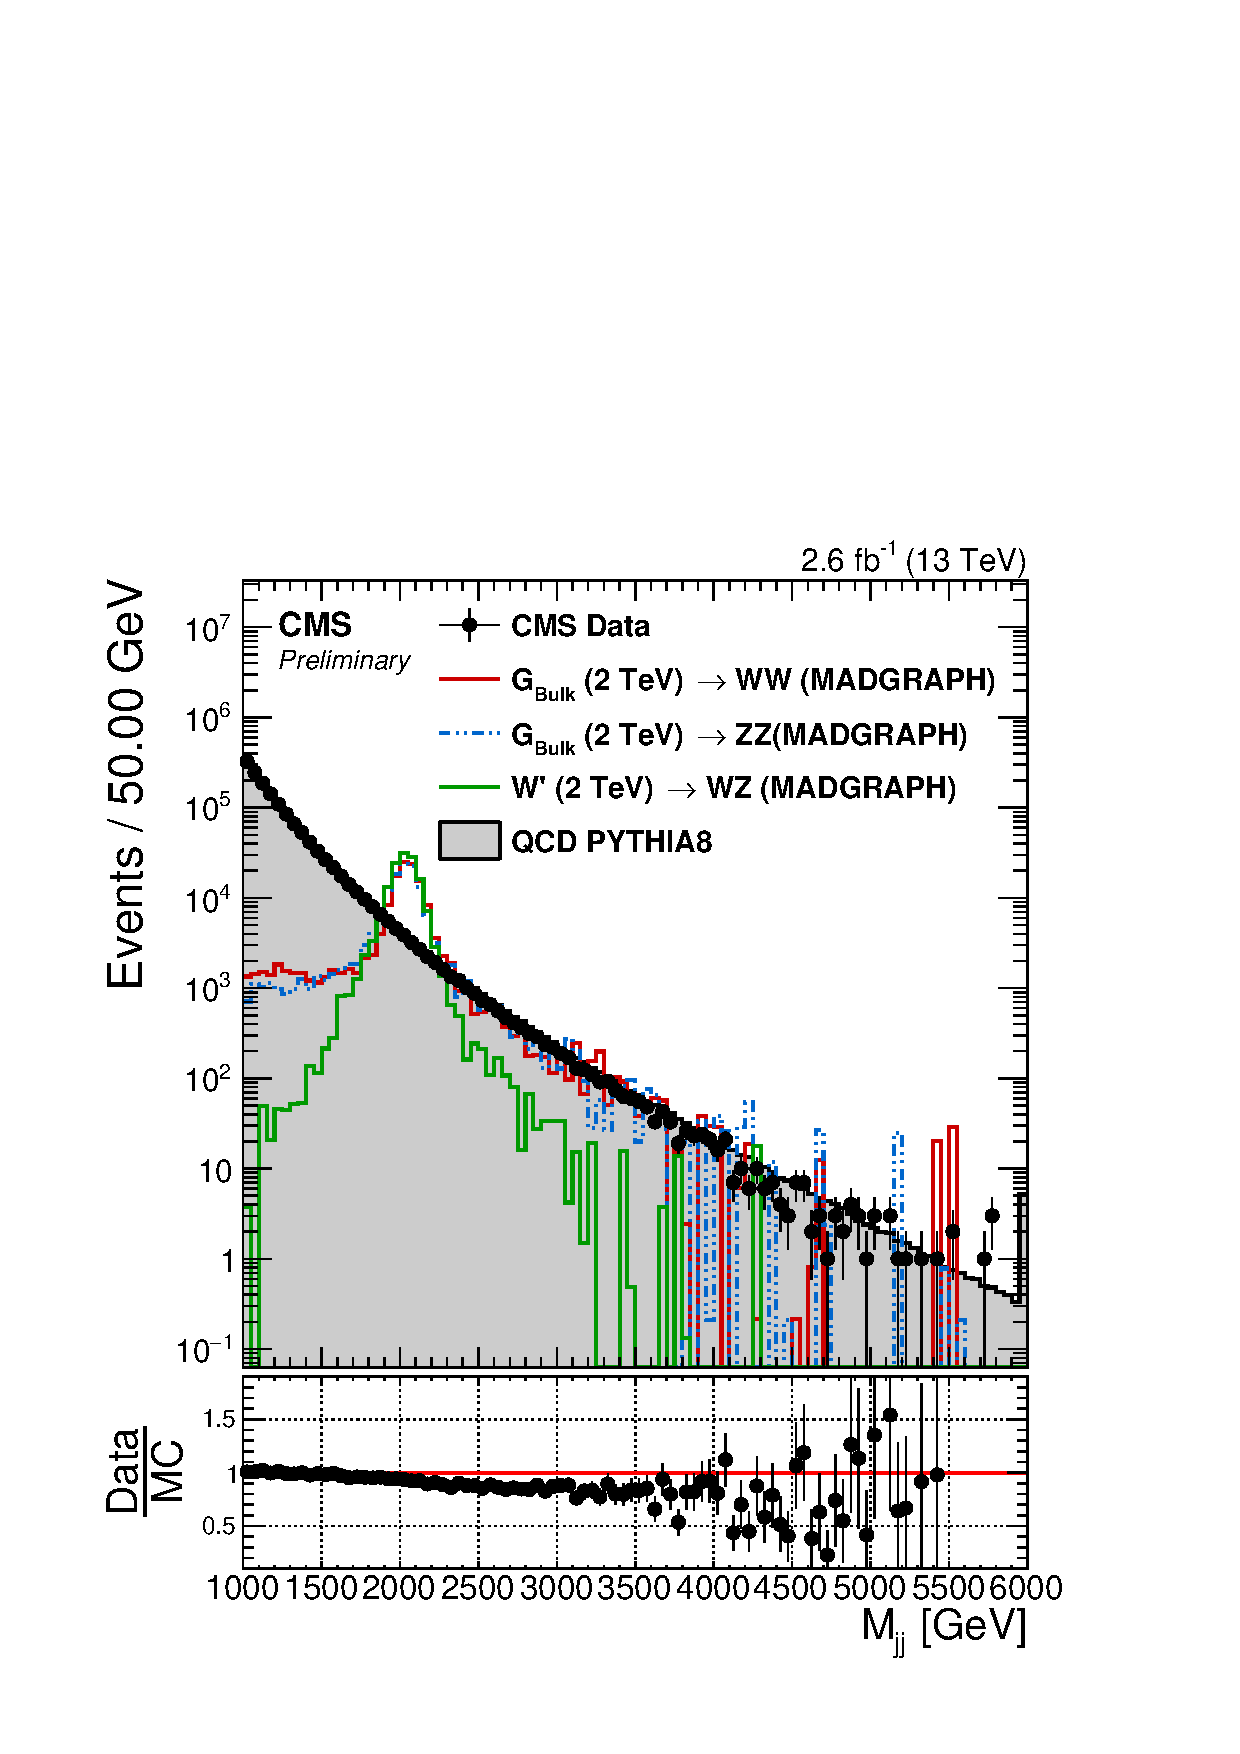
\includegraphics[width=0.4\textwidth]{figures/analysis/search1/AN-15-211/controlplots/silverjson/Mjj_WSignal.pdf}
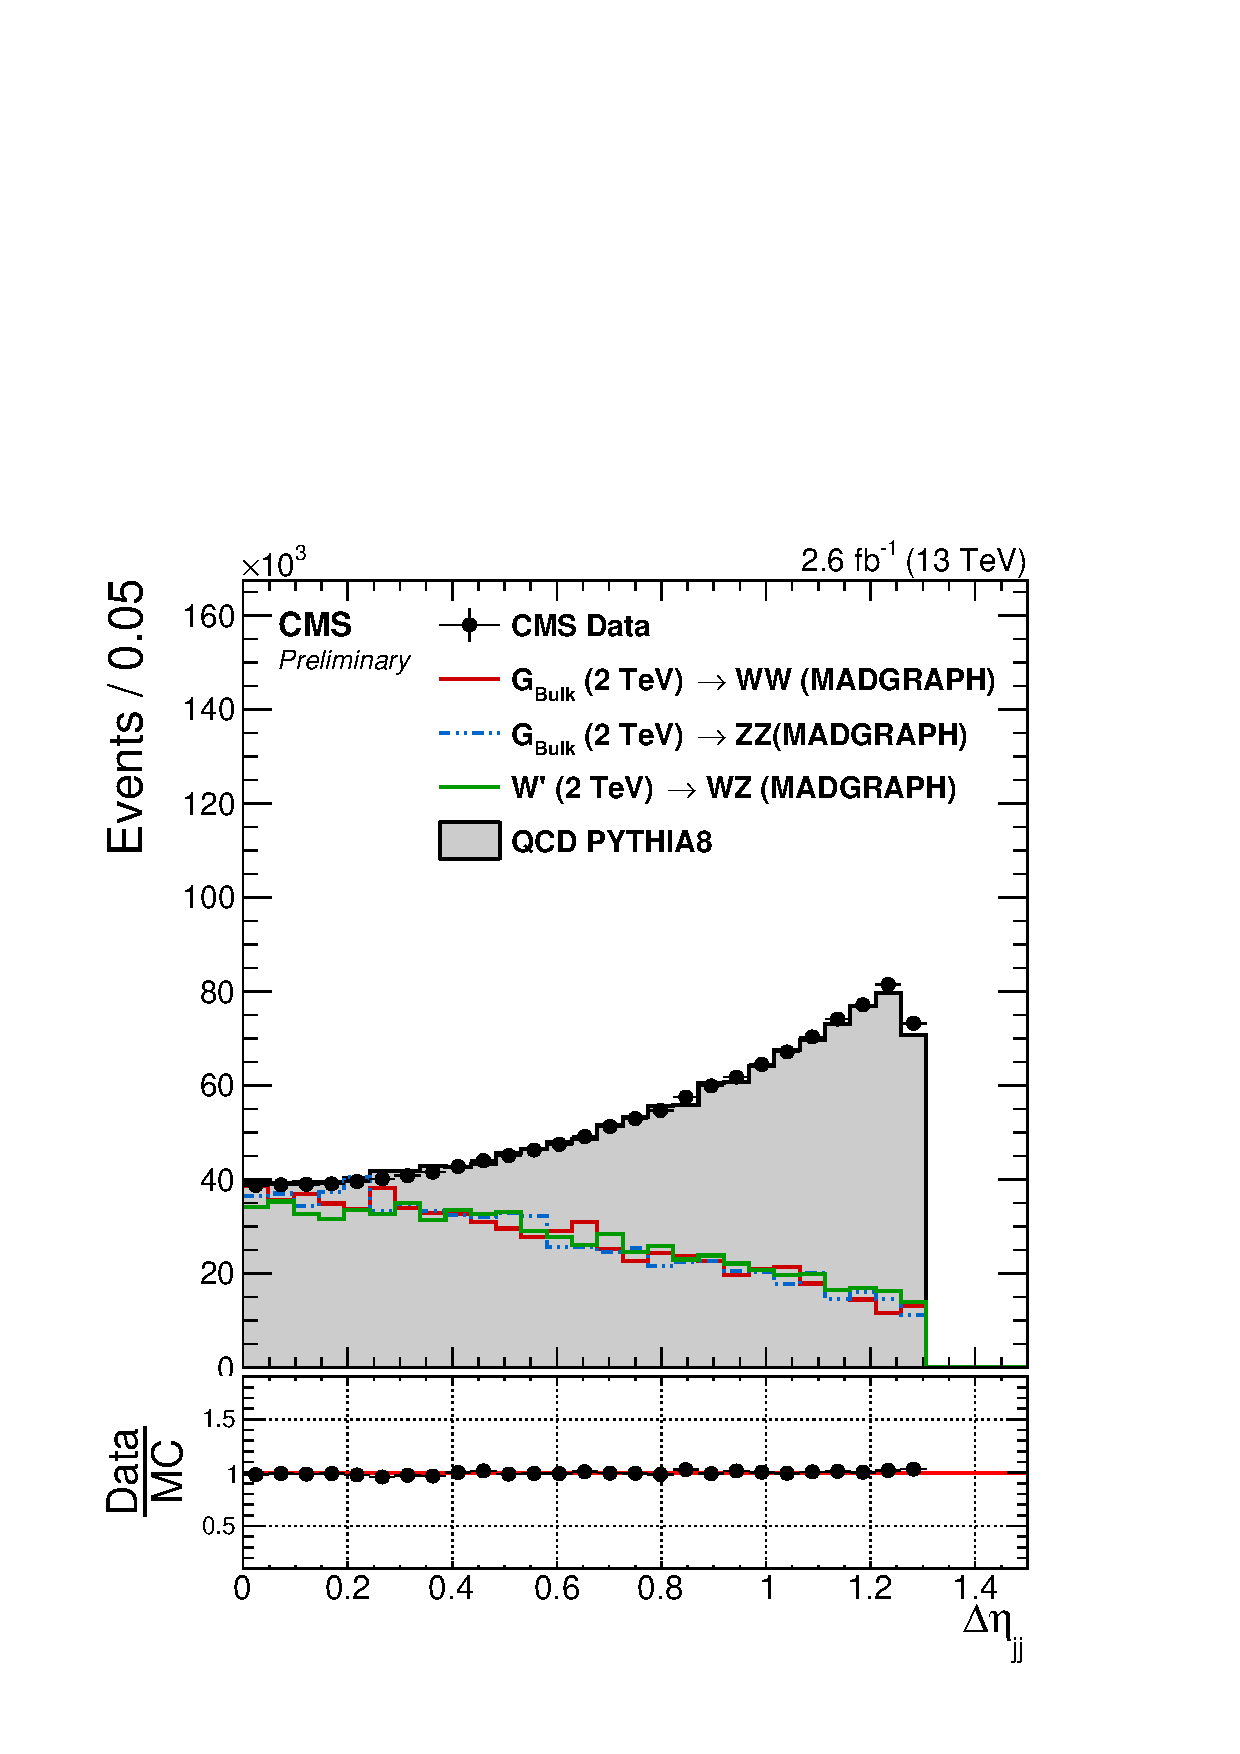
\includegraphics[width=0.4\textwidth]{figures/analysis/search1/AN-15-211/controlplots/silverjson/DeltaEta_WSignal.pdf}
\caption{Jet \PT (top left), $\eta$ (top right), dijet invariant mass (bottom left) and $|\Delta \eta|_{jj}$ (bottom right) distribution for the two leading jets in the event after loose preselections are applied. The signal is scaled by an arbitrary number.}
\label{fig:kinematics-all}
\end{figure}

\subsection{Vector boson tagging}
\label{sec:searchI:wtagging}
After preselections, we take advantage of the jet substructure algorithms described in Section~\ref{sec:objreco:substructure} to further separate boosted W/Z jets from the QCD multijet background. In the 8 \TeV analysis~\cite{Khachatryan:1700394} published the previous year, the pruning algorithm was the chosen grooming algorithm of CMS. However, recent progress had been made in the development of alternative grooming algorithms that had favorable properties from a theoretical point of view (see Sections~\ref{sec:objreco:grooming} and ~\ref{sec:searchII:puppisoftdrop}). We therefore studied two different grooming algorithms: pruning and softdrop (with $\beta=0$ and $z_{cut} = 0.1$). A comparison of the jet mass for W, Z, and H jets after either the softdrop (dotted lines) or pruning (solid lines) algorithms were applied is shown in Figure~\ref{fig:searchI:sdvspruning}.
 \begin{figure}[h!]
 \centering
 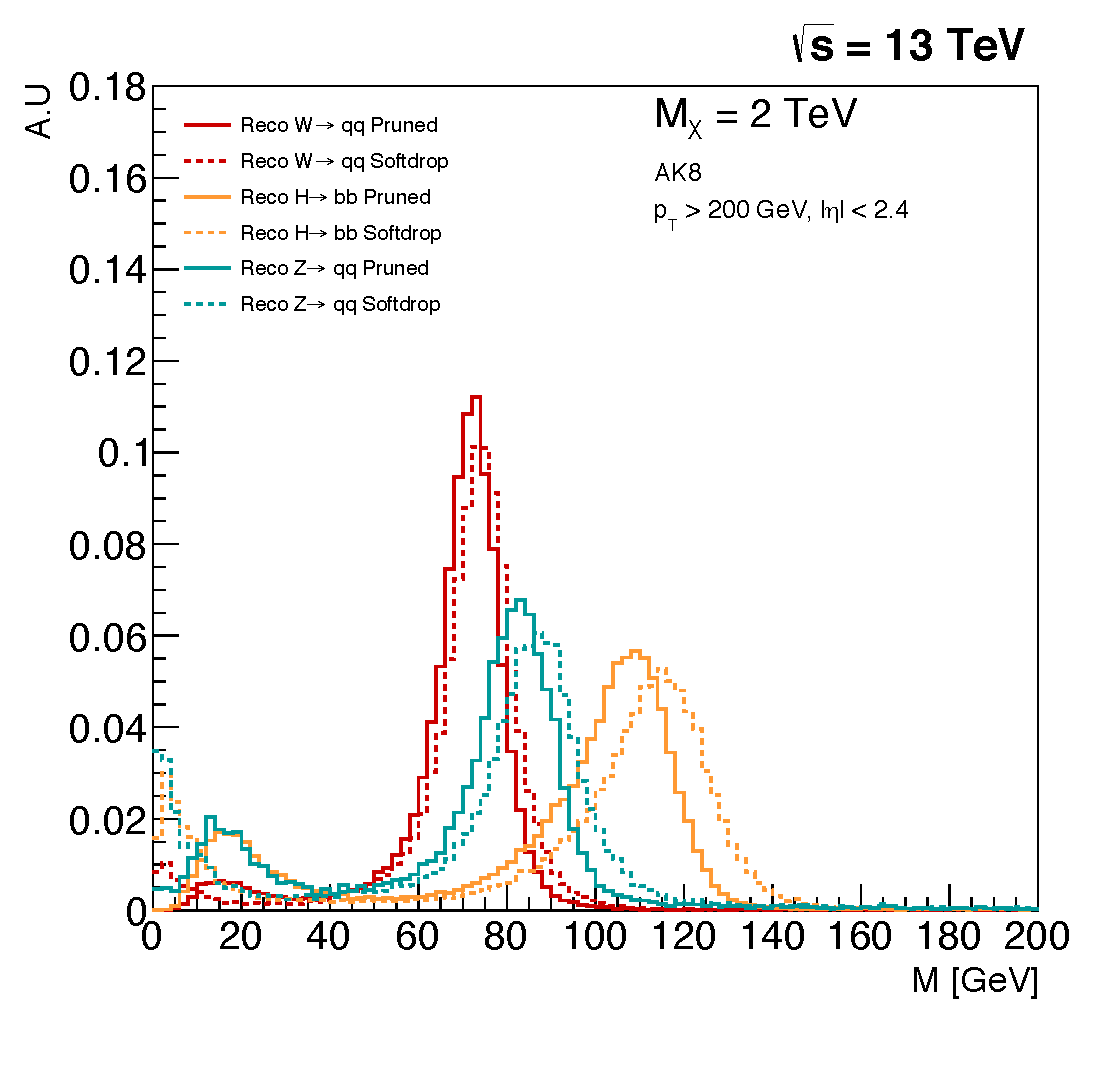
\includegraphics[width=0.49\textwidth]{figures/analysis/search1/misc/SDvsPruned.pdf}
 \caption{The softdrop (dotted lines) and the pruned (solid lines) jet mass for \PW, \PZ and \PH jets.}
 \label{fig:searchI:sdvspruning}
 \end{figure}
One of the first observations we made comparing the two grooming algorithms was that there appeared to be a strong dependence of the softdrop mass on the jet \PT. Figure~\ref{fig:searchI:grommedmassshift} shows the pruned (left) and softdrop (right) mass distributions for \PW jets coming from the decay of a \BulkG with a resonance mass of $0.8 \TeV < \mX < 4 \TeV$. While the pruned jet mass mean appeared stable as the jet transverse momenta of the jet increased ($\PT\sim\mX/2$), the mean of the softdrop jet mass shifted towards lower values as jet \PT increased.
\begin{figure}[h!]
\centering
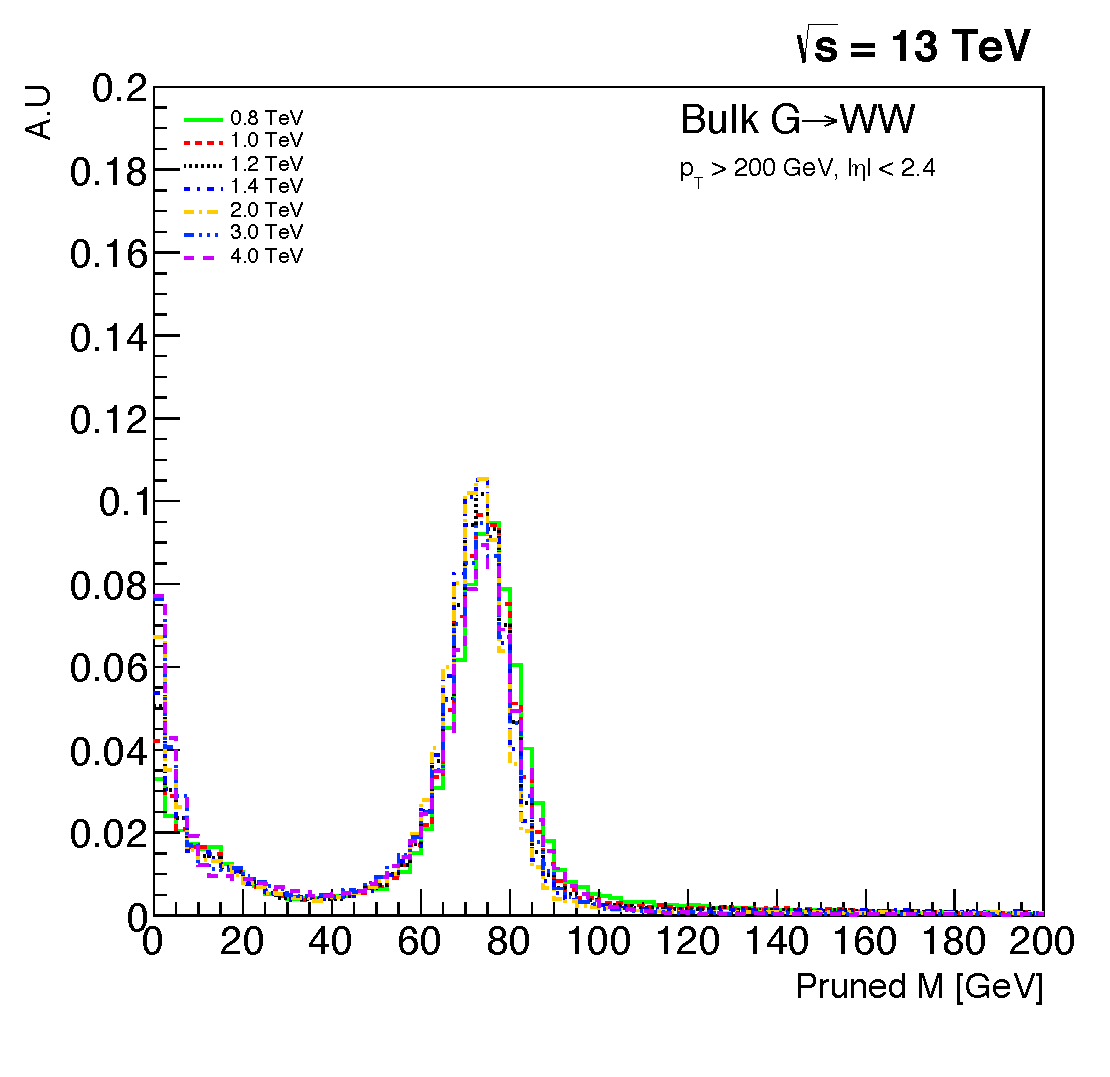
\includegraphics[width=0.49\textwidth]{figures/analysis/search1/misc/pruned_mass_shift.pdf}
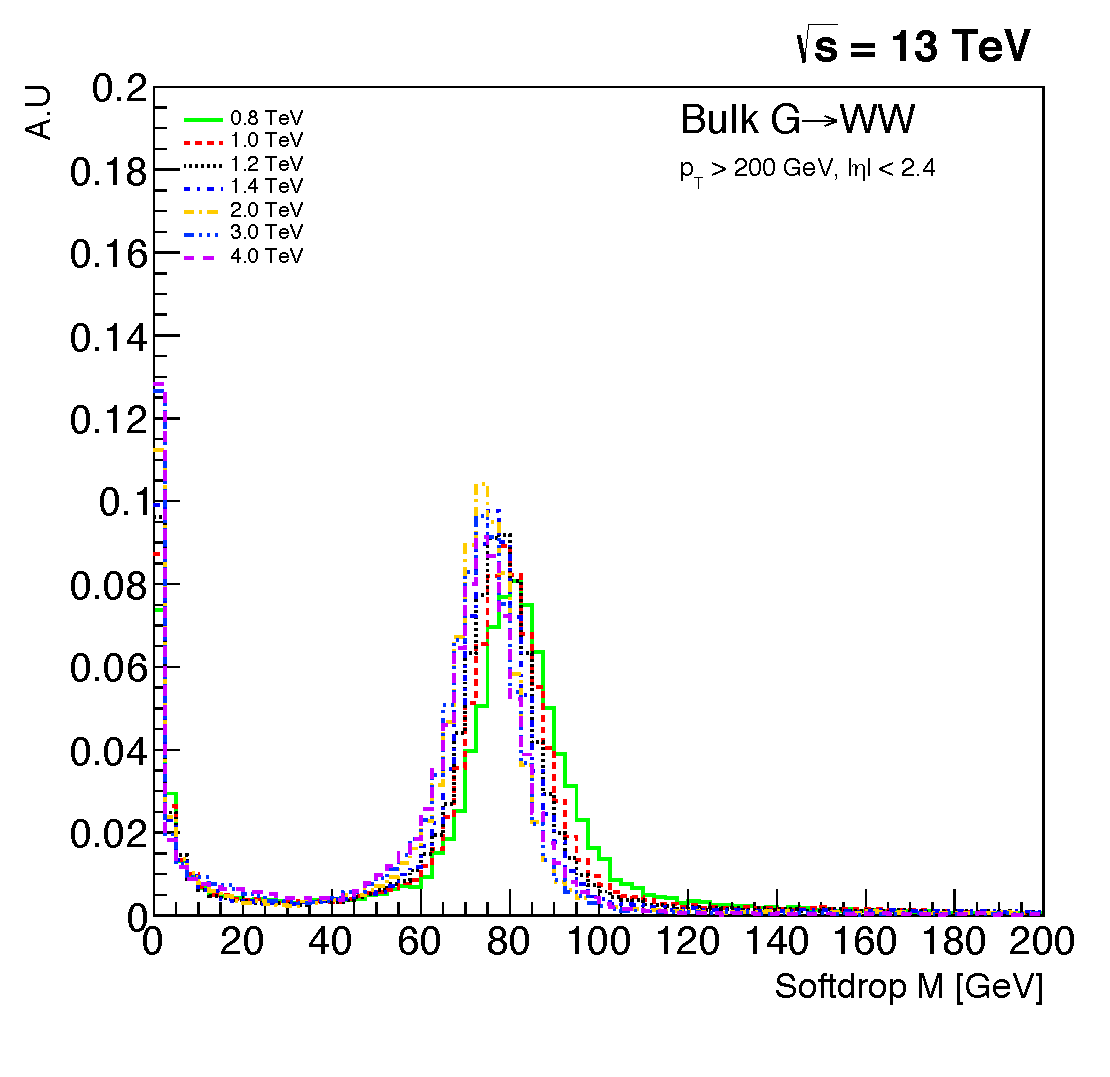
\includegraphics[width=0.49\textwidth]{figures/analysis/search1/misc/softdrop_mass_shift.pdf}
\caption{The jet mass distribution for W jets coming from a $\textrm{G}_{\textrm{bulk}}$ of masses in the range $0.8 \TeV < \mX < 4 \TeV$ decaying to \WW, here with pruning applied (left) and softdrop (right). A strong shift in the jet mass mean as a function of \PT ($\sim\mX/2$), is observed for jets groomed with the softdrop algorithm. Charge hadron subtraction is applied to all jets before clustering.}
\label{fig:searchI:grommedmassshift}
\end{figure}
In order to investigate whether this was a reconstruction effect or an algorithmic effect, we additionally looked at the pruned and softdrop mass for generator-level jets (jets clustered with generator-level particles not passed through the detector simulation). Figure~\ref{fig:searchI:grommedmassshift_genvsreco} shows the reconstructed (solid line) and generator-level (dotted line) jet mass distributions after pruning (left) or softdrop (right) have been applied. Again, the distributions are compared for jets with very different \PT profiles, here for W jets coming from a $\BulkG \rightarrow \WW$ of mass 0.8 \TeV (red) yielding a \PT of about 400 GeV, and a mass of 2.0 TeV, yielding a \PT of about 1 TeV. Interestingly, we observe a \PT-dependent mass shift already for generator level softdrop jets (comparing the dotted lines in the right plot), an effect further enhanced at reconstruction level. This effect is not present for pruned jets, for either generator level or reconstruction level.
\begin{figure}[h!]
\centering
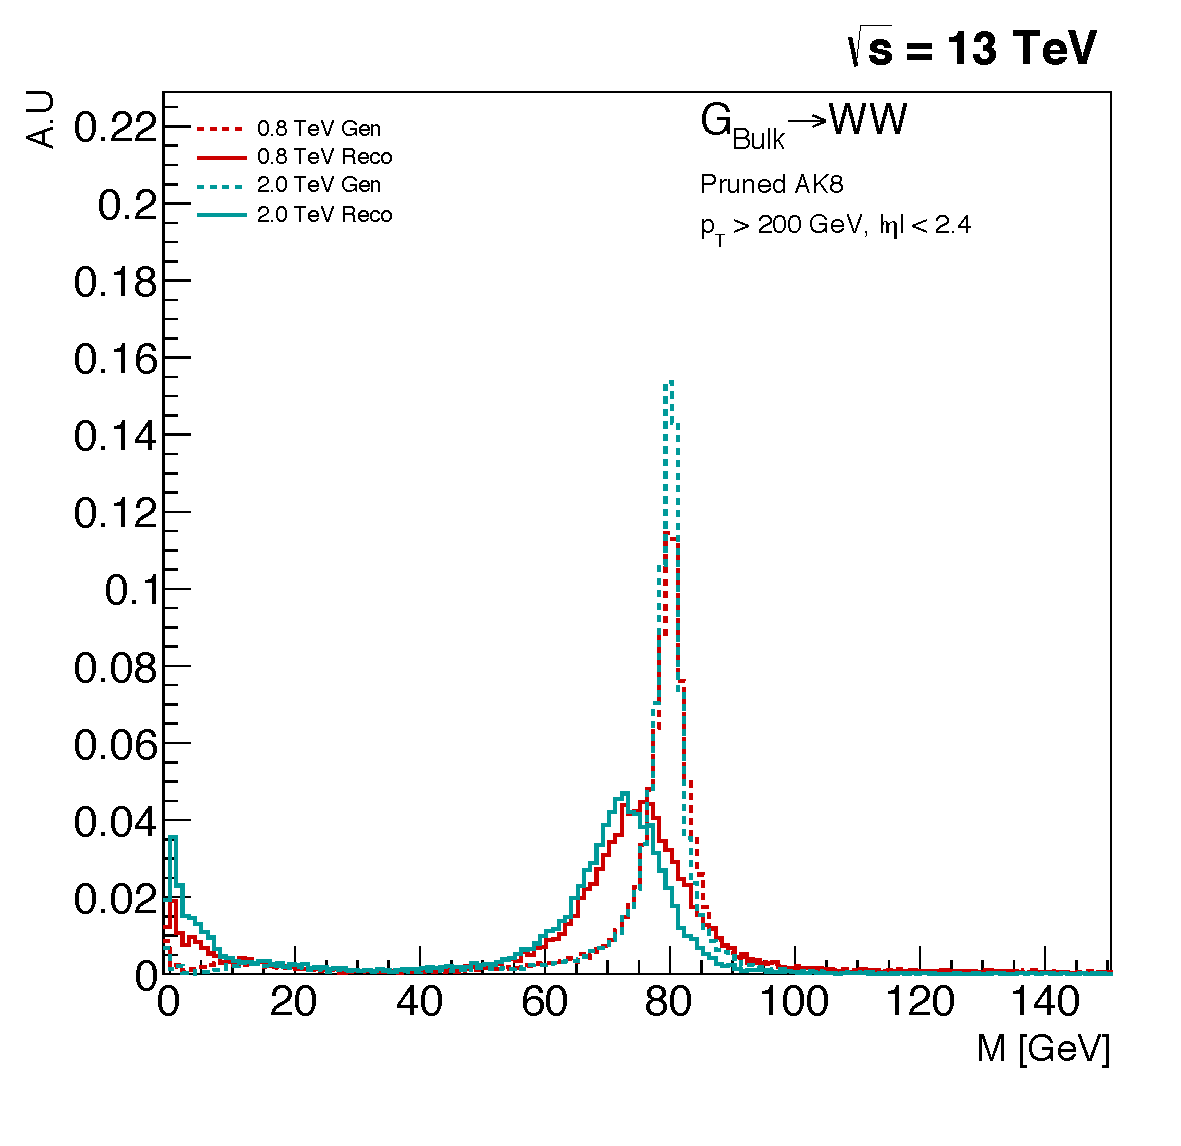
\includegraphics[width=0.49\textwidth]{figures/analysis/search1/misc/pruned_mass_shift_genvsreco.pdf}
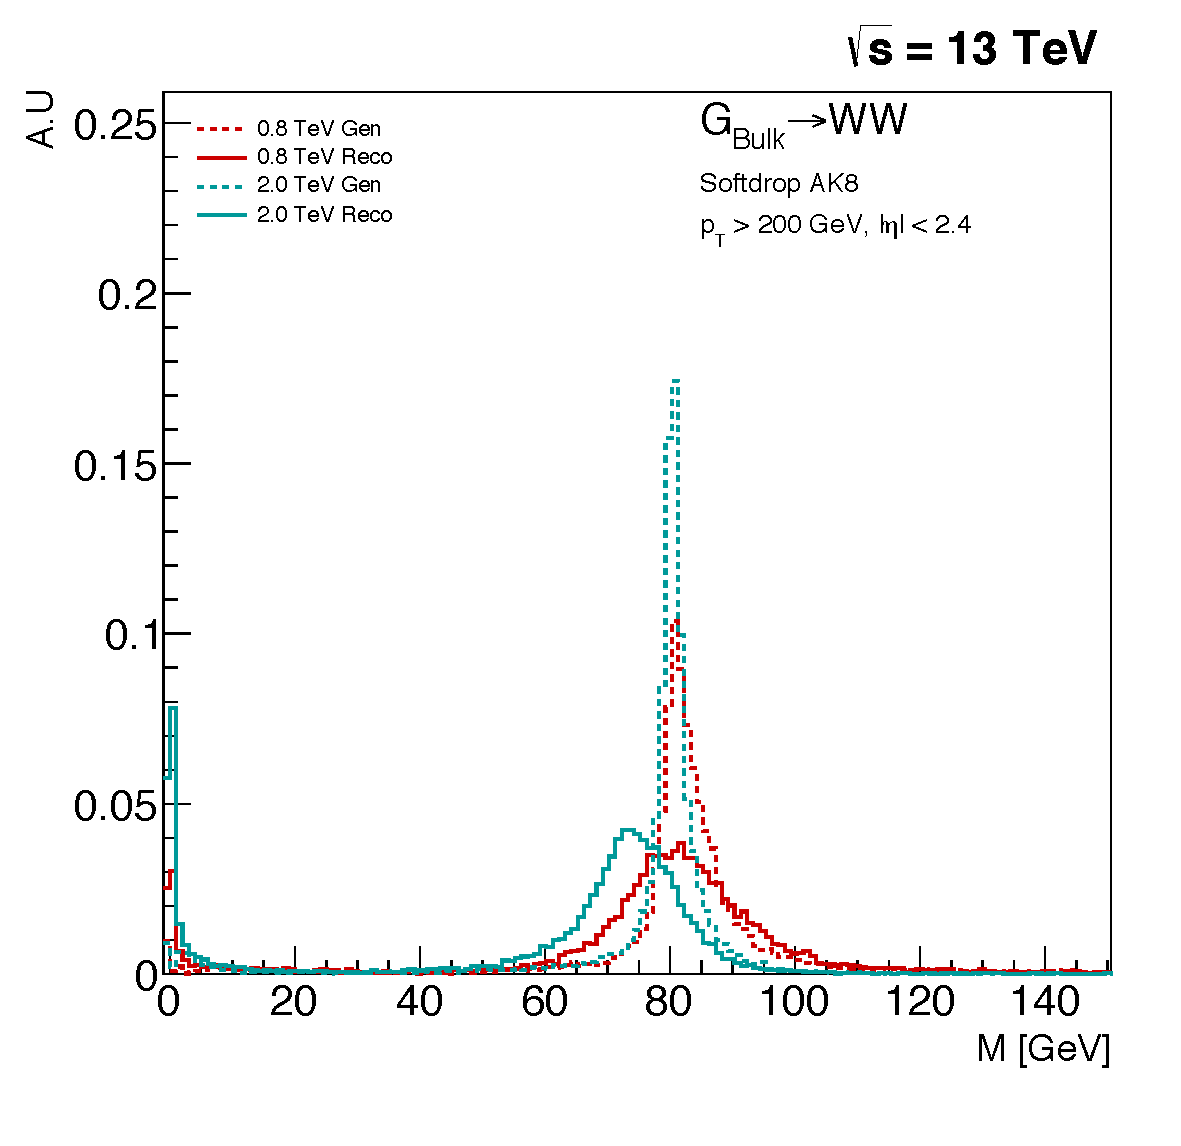
\includegraphics[width=0.49\textwidth]{figures/analysis/search1/misc/softdrop_mass_shift_genvsreco.pdf}
\caption{The reconstructed (solid line) and generator level (dotted line) jet mass distribution for W jets coming from a $\BulkG \rightarrow \WW$ of mass $\mX = 0.8 \TeV$ (red), roughly $\PT\sim 400 \GeV$, and $\mX = 2.0 \TeV$ (blue), $\PT\sim 1 \TeV$. Here for the pruned (left) and softdrop (right) jet mass.}
\label{fig:searchI:grommedmassshift_genvsreco}
\end{figure}
The observed \PT-dependence of the softdrop mass was problematic due to the fact that it would require a \PT-dependent mass window. This would again require several different measurements to produce an efficiency scale factor between simulation and data, for each mass window, or a significantly higher uncertainty on the signal yield. Due to these findings, the grooming algorithm of choice for this analysis is pruning, with the signal selection window defined as $65 \GeV < m_{p} < 105 \GeV$. The above findings will be important for subsequent analyses and are revisited in Section~\ref{searchII}.\par
The variable used to determine the substructure of the V jets is the n-subjettiness ratio \nsubj, as described in Section~\ref{sec:objreco:nsubj}. The \nsubj variable is correlated to the pruned jet mass, however, it still provides additional signal discrimination when applied after the pruned jet mass selection. Figure~\ref{fig:searchI:tau21_groomedvsungroomed} shows the \nsubj distribution for the QCD background and W jets from a signal decay before (left) and after (right) a pruned mass cut of $65 \GeV < m_{p} < 105 \GeV$ has been applied.
\begin{figure}[h!]
\centering
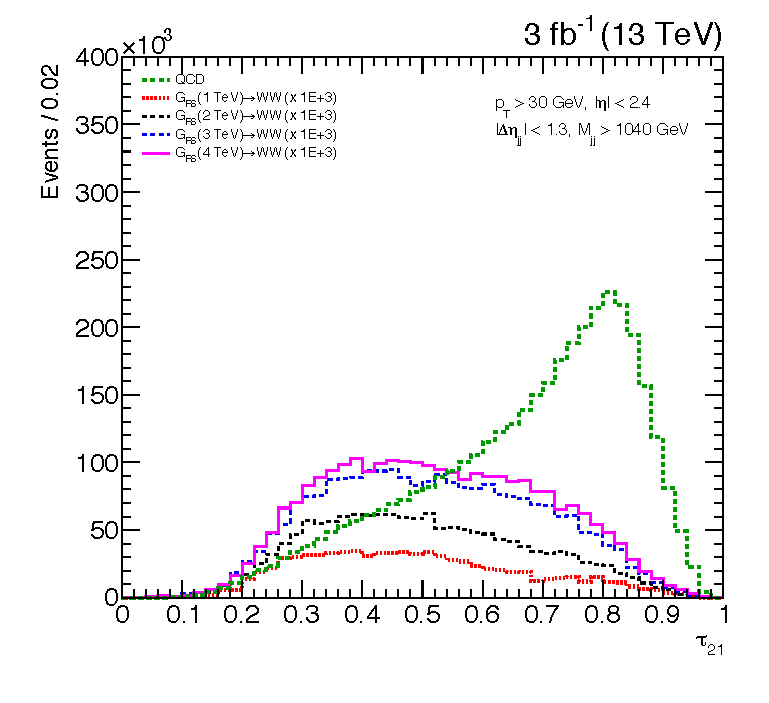
\includegraphics[width=0.49\textwidth]{figures/analysis/search1/misc/tau21_ungroomed.pdf}
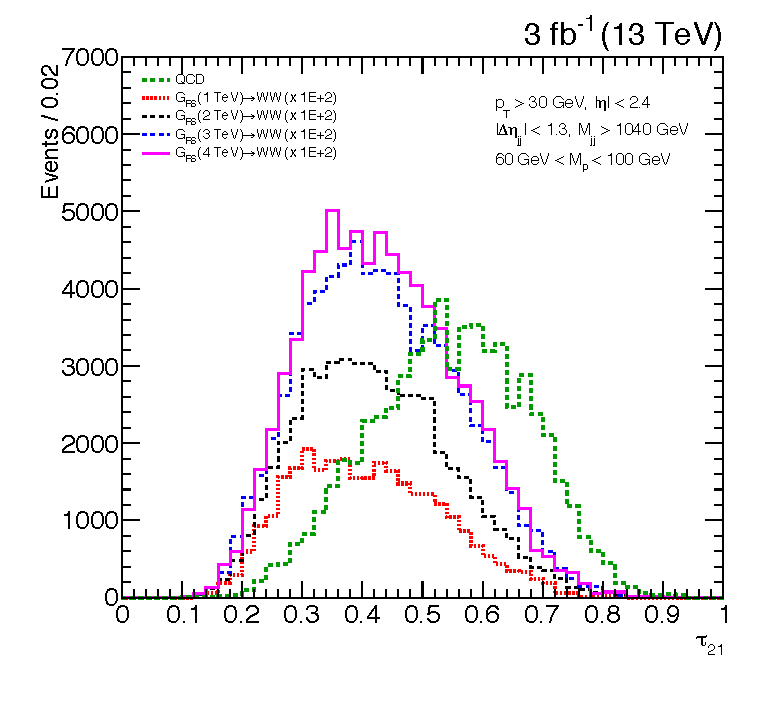
\includegraphics[width=0.49\textwidth]{figures/analysis/search1/misc/tau21_groomed.pdf}
\caption{The \nsubj distribution for QCD background and signal jets before (left) and after (right) a pruned mass window is applied. The discriminating power of \nsubj is strongly reduced after grooming.}
\label{fig:searchI:tau21_groomedvsungroomed}
\end{figure}
\noindent We perform a cut optimization on \nsubj after all analysis selections, including the pruned mass window of $65 \GeV < m_{p} < 105 \GeV$, have been applied. This is done by scanning over thresholds for the \nsubj variable, and for each threshold, computing the Punzi significance~\cite{Punzi:2003bu} defined as
\begin{equation*}
\textrm{S} = \frac{\epsilon_S}{1+\sqrt{\textrm{B}}}  ,
\end{equation*}  
where $\epsilon_S$ is the signal efficiency and B is the total number of background events. The selection with the highest significance is defined as the optimal value. The signals under consideration are W jets coming from the decay of a \BulkG with $1 \TeV< mX < 4 \TeV$, against a background of light-flavored QCD jets. Only jets with a dijet invariant mass in a 20\% window around the resonance mass are considered. The Punzi significance as a function of the upper cut value on \nsubj is shown on the left in Figure~\ref{fig:searchI:tau21_punzi}.
\begin{figure}[h!]
\begin{center}
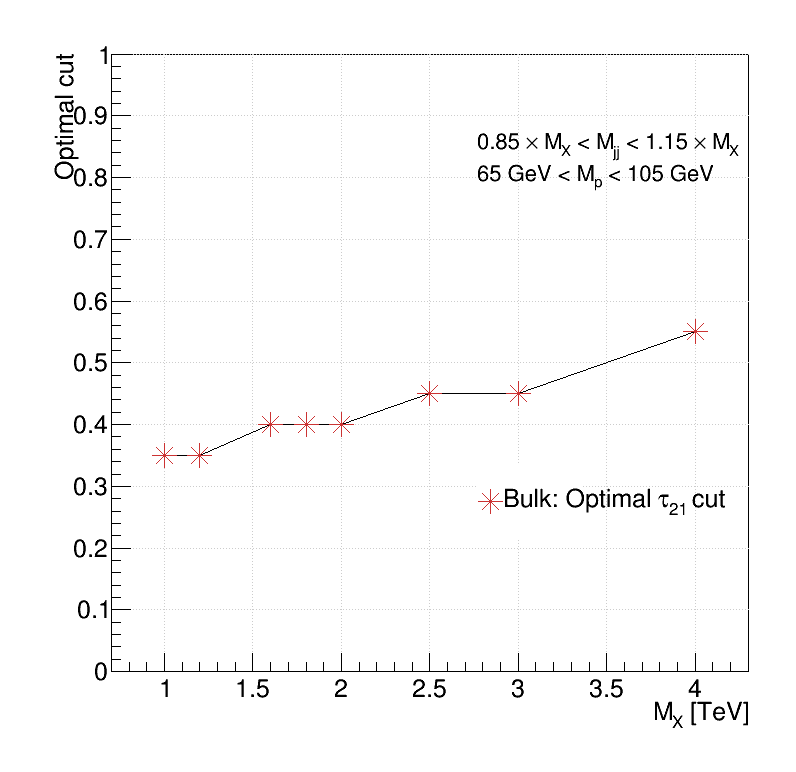
\includegraphics[width=0.49\textwidth]{figures/analysis/search1/AN-15-196/tau21optimisation/HP_Punzi_BulkWW.png}
%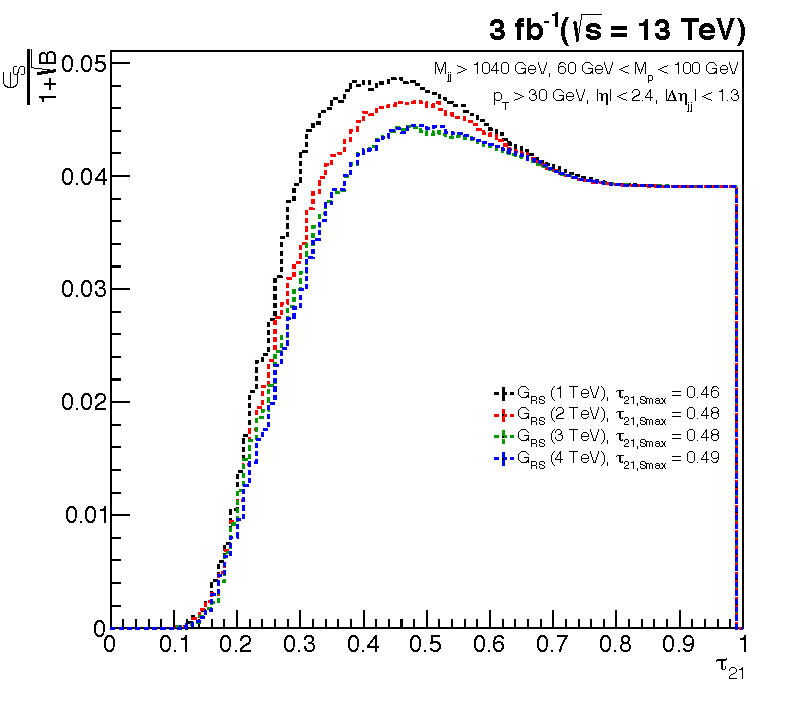
\includegraphics[width=0.49\textwidth]{figures/analysis/search1/misc/tau21_punzi.pdf}
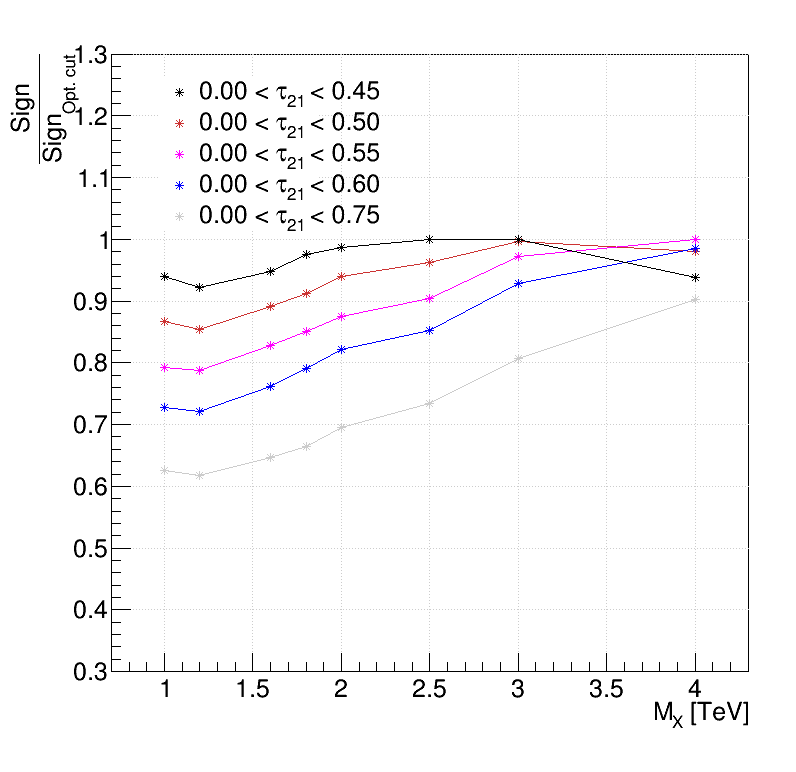
\includegraphics[width=0.49\textwidth]{figures/analysis/search1/AN-15-196/tau21optimisation/HP_CutSignificance_bulkWW.png}\\
\caption{Left: Optimal upper value of \nsubj for selecting the signal as a function of \BulkG mass. Right: The ratio of a given \nsubj cut over the significance of the best cut at that mass value.}
\label{fig:searchI:tau21_punzi}
\end{center}
\end{figure}
The optimal cut gets looser as the dijet invariant mass increases, something which can be understood when looking at the QCD dijet invariant mass spectrum in Figure~\ref{fig:kinematics-all}. The number of QCD jets falls off exponentially with \mjj, meaning that the background at 4 \TeV is considerably lower than at 1 \TeV. This allows for a looser cut on \nsubj as \mjj increases. In order to choose a single cut which works reasonably well for all values of resonance mass, we look at the ratio of a given \nsubj cut over the significance of the best cut at that mass value. This is shown in the right plot of Figure~\ref{fig:searchI:tau21_punzi}. Choosing signal events with a $\nsubj < 0.45$ yields the most stable performance out of the investigated \nsubj selection requirements and also maintains low background rates at low \mjj. This selection is therefore used for our main analysis category. In order to account for the fact that background rates are lower for higher values of \mjj, we add an additional analysis category, $0.45 < \nsubj < 0.75$, which contains $>95\%$ of the signal and enhances the analysis sensitivity in the case when the background is low. These categories are hereafter referred to as the \emph{high-purity} (HP) category, for jets with $0<\tau_{21} \leq 0.45$, and the \emph {low-purity} (LP) category, for jets with $0.45<\tau_{21}\leq0.75$. QCD jets from light-flavor quarks and gluons (u,d,s,g) can be incorrectly identified as W-jets, and these events are referred to as "mistags" of the W-tagger. The W-tagging efficiency and QCD light-flavored jet mistagging rate for a W-tagger consisting of $0<\tau_{21} \leq 0.45$ and  $65 \GeV < m_{p} < 105 \GeV$ is shown in Figure~\ref{fig:searchI:wtageff}, both as a function of jet \PT and as a function of number of primary vertices in the event.
\begin{figure}[h]
\begin{center}
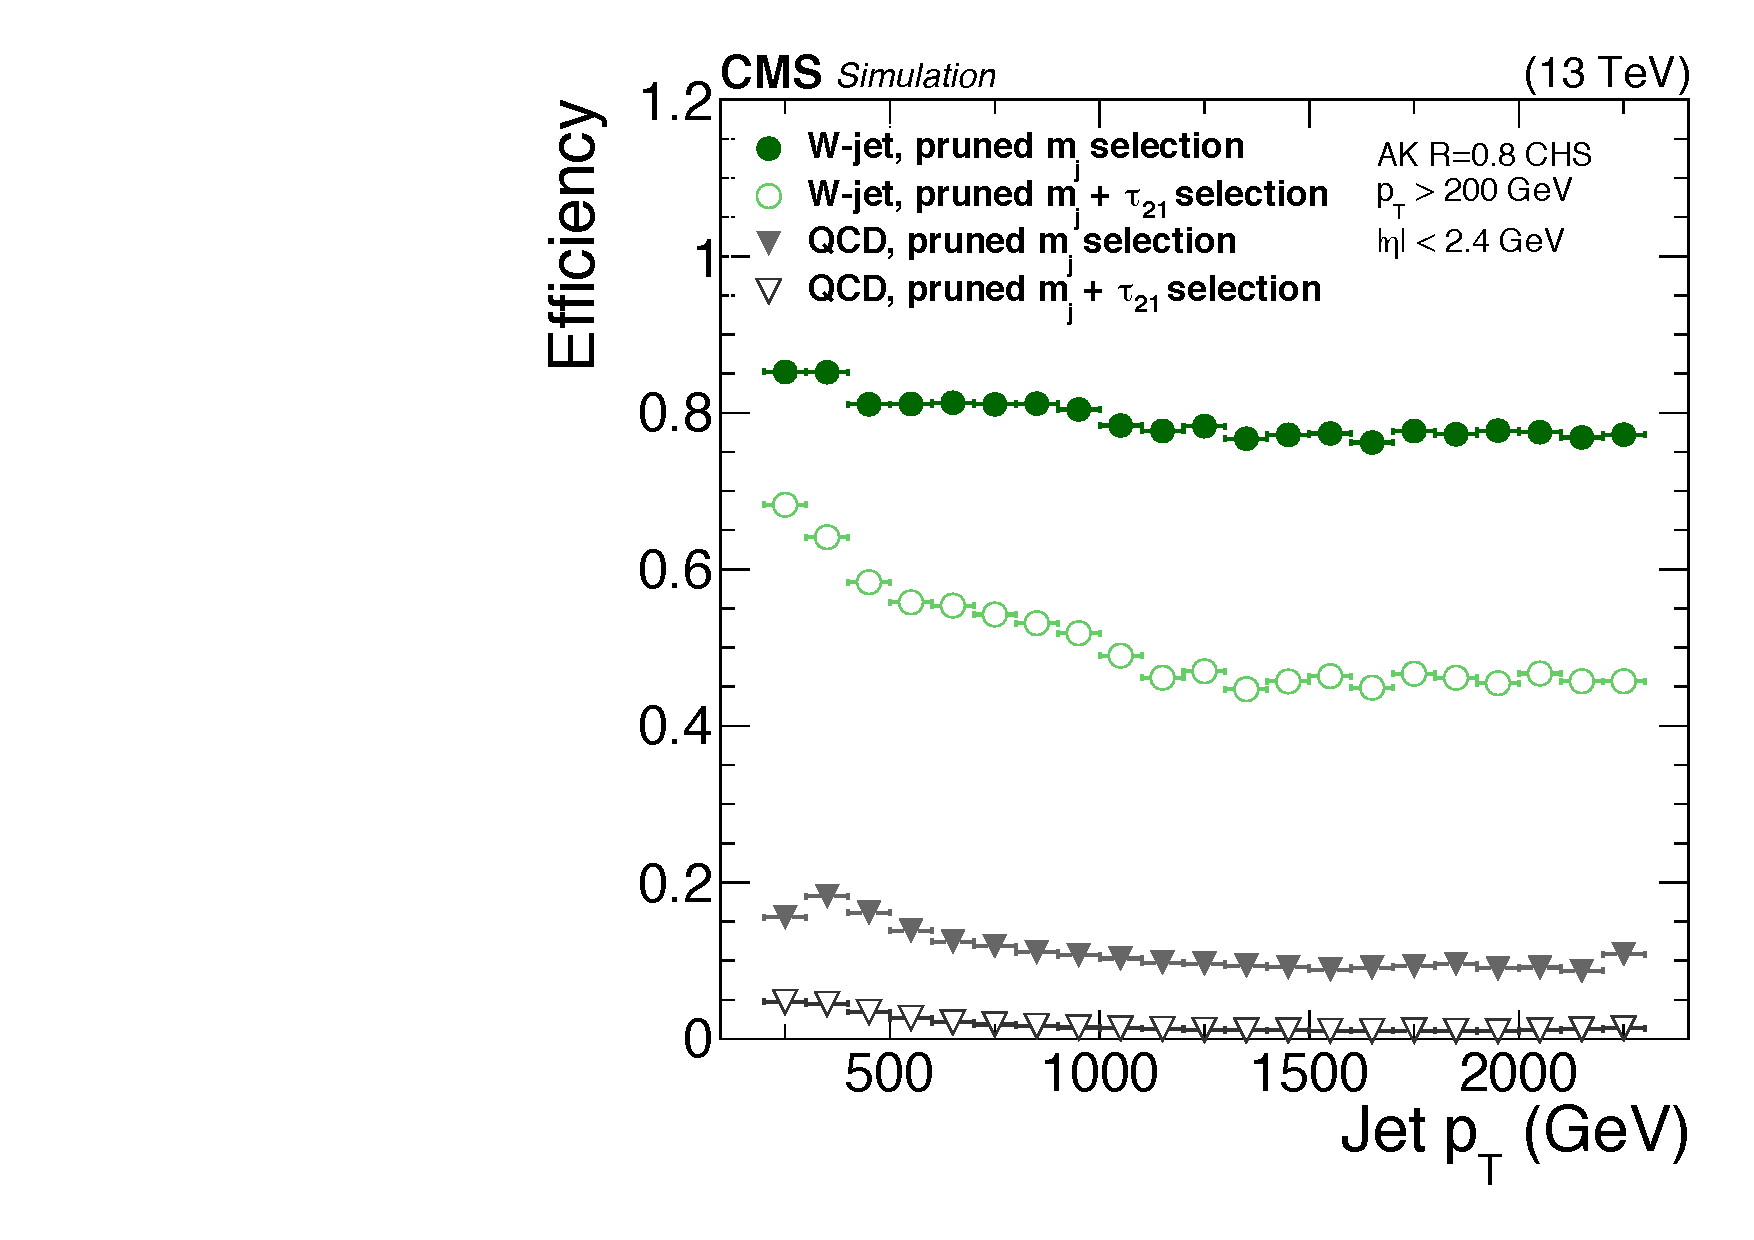
\includegraphics[width=0.49\textwidth]{figures/analysis/search1/misc/WtagSigEff_vpT_pruned.pdf}
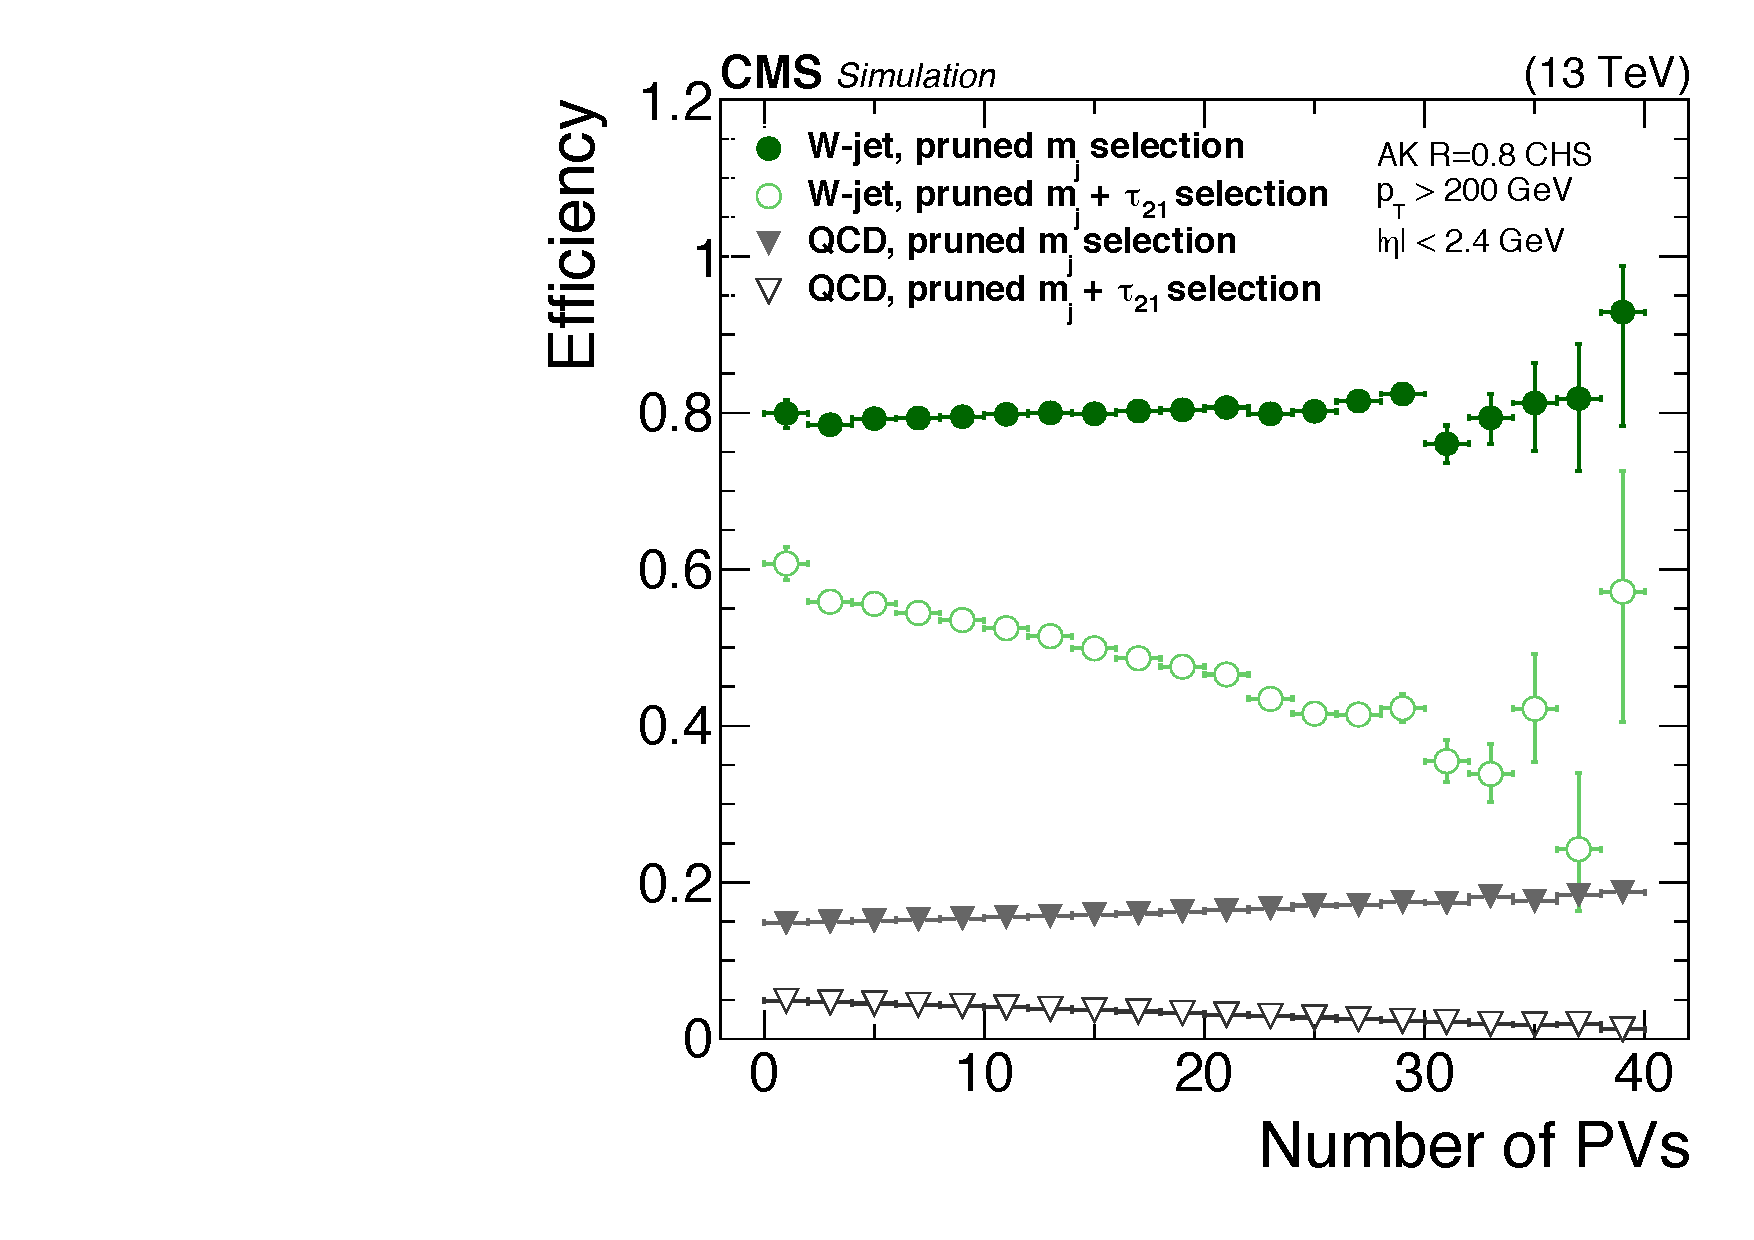
\includegraphics[width=0.49\textwidth]{figures/analysis/search1/misc/WtagSigEff_vnPVs_pruned.pdf}
\caption{The W-tagging efficiency (green) and light jet mistag rate (grey) for a selection based on either the pruned jet mass or the pruned jet mass and \nsubj as a function of \PT (left) and the number of primary vertices (right).}
\label{fig:searchI:wtageff}
\end{center}
\end{figure}
The signal efficiency when applying only the pruned jet mass selection is around 80\% with a mistag rate of $\sim 15\%$. After applying the \nsubj selection, the signal efficiency drops to around 55\% and the mistagging rate to $\sim 2\%$. Another interesting feature is the dependence of \nsubj on jet \PT and pileup, compared to the resilience of the groomed mass as a function of the same variables. This will be another feature we explore in the second analysis (Section~\ref{searchII}). Figure~\ref{fig:wtag} shows the pruned jet mass (left) and the $\tau_{21}$ distribution (right) for signal and background Monte Carlo, as well as the distributions measured in data. 
\begin{figure}[h!]
\centering
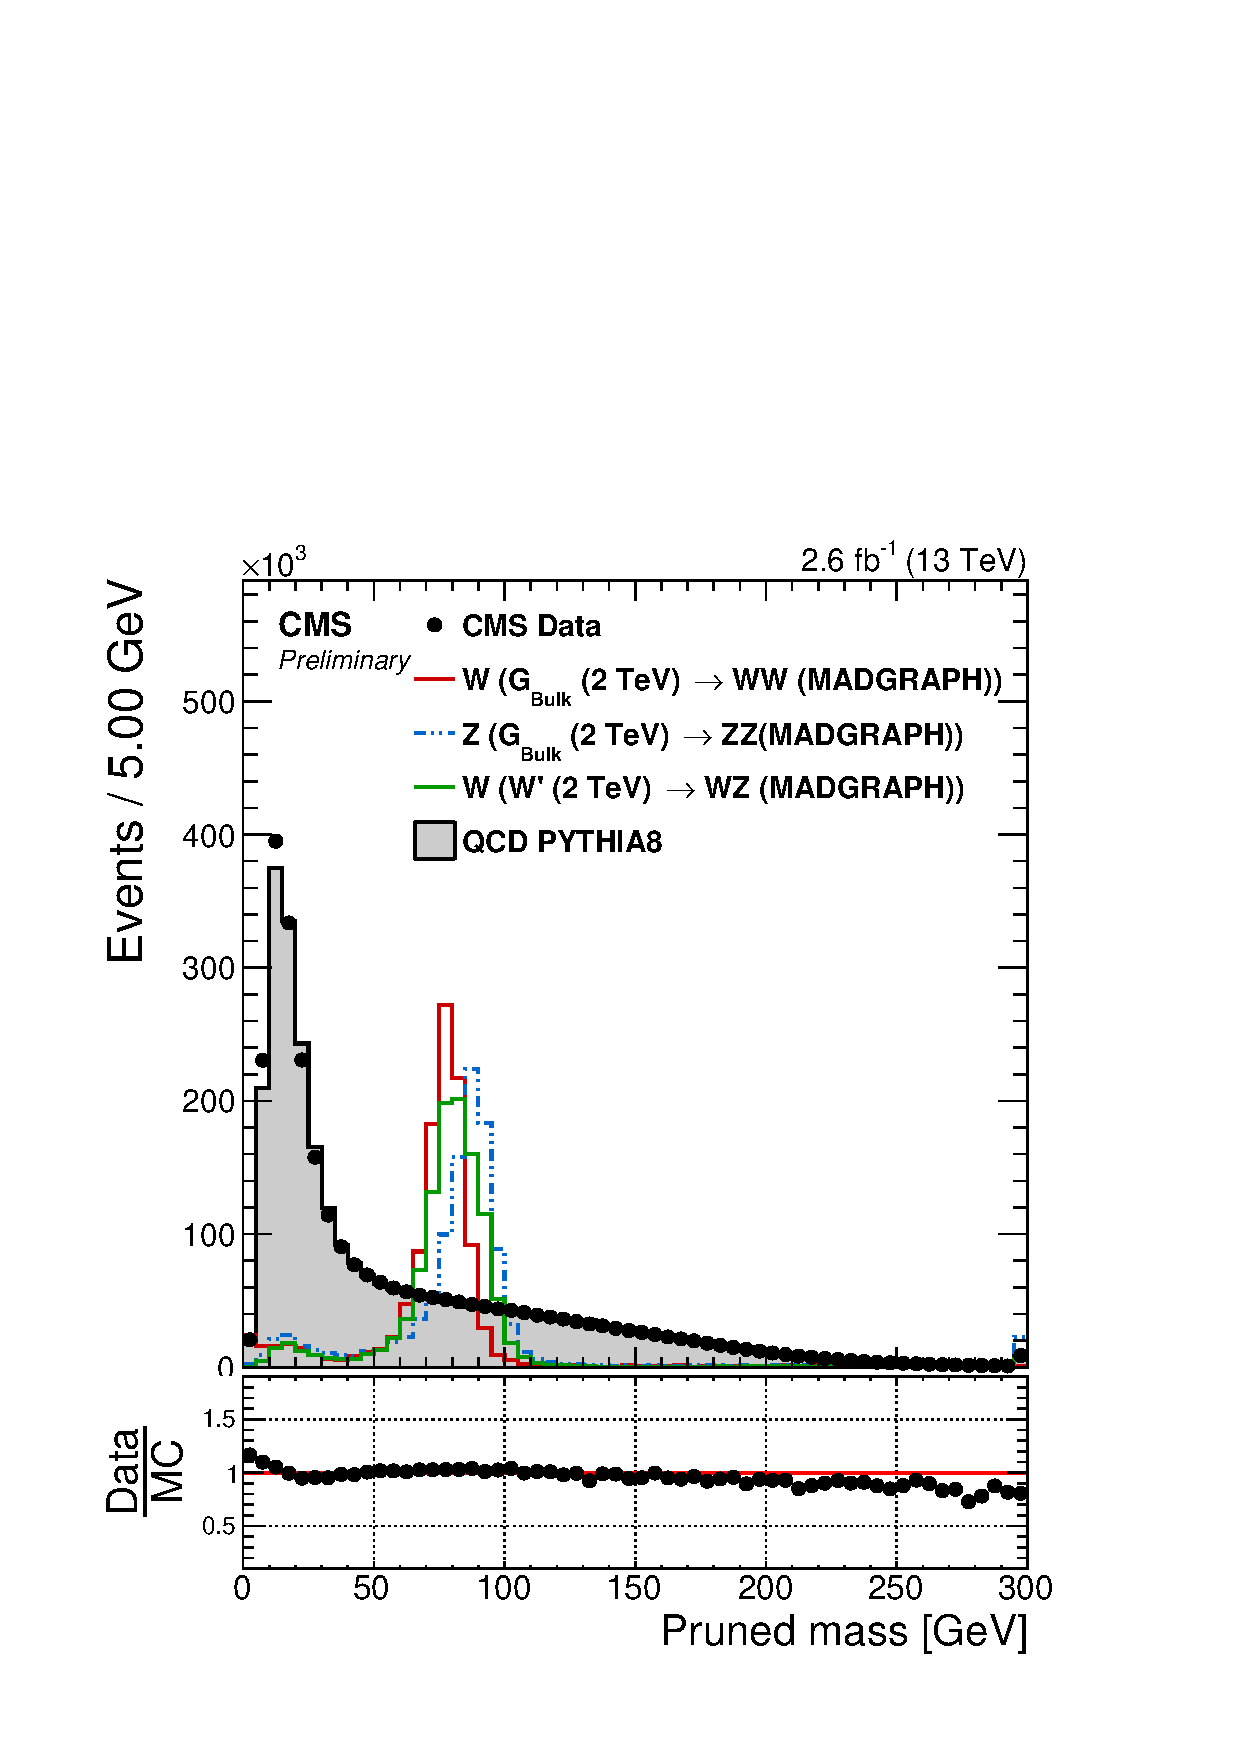
\includegraphics[width=0.4\textwidth]{figures/analysis/search1/AN-15-211/controlplots/silverjson/PrunedMass_WSignal.pdf}
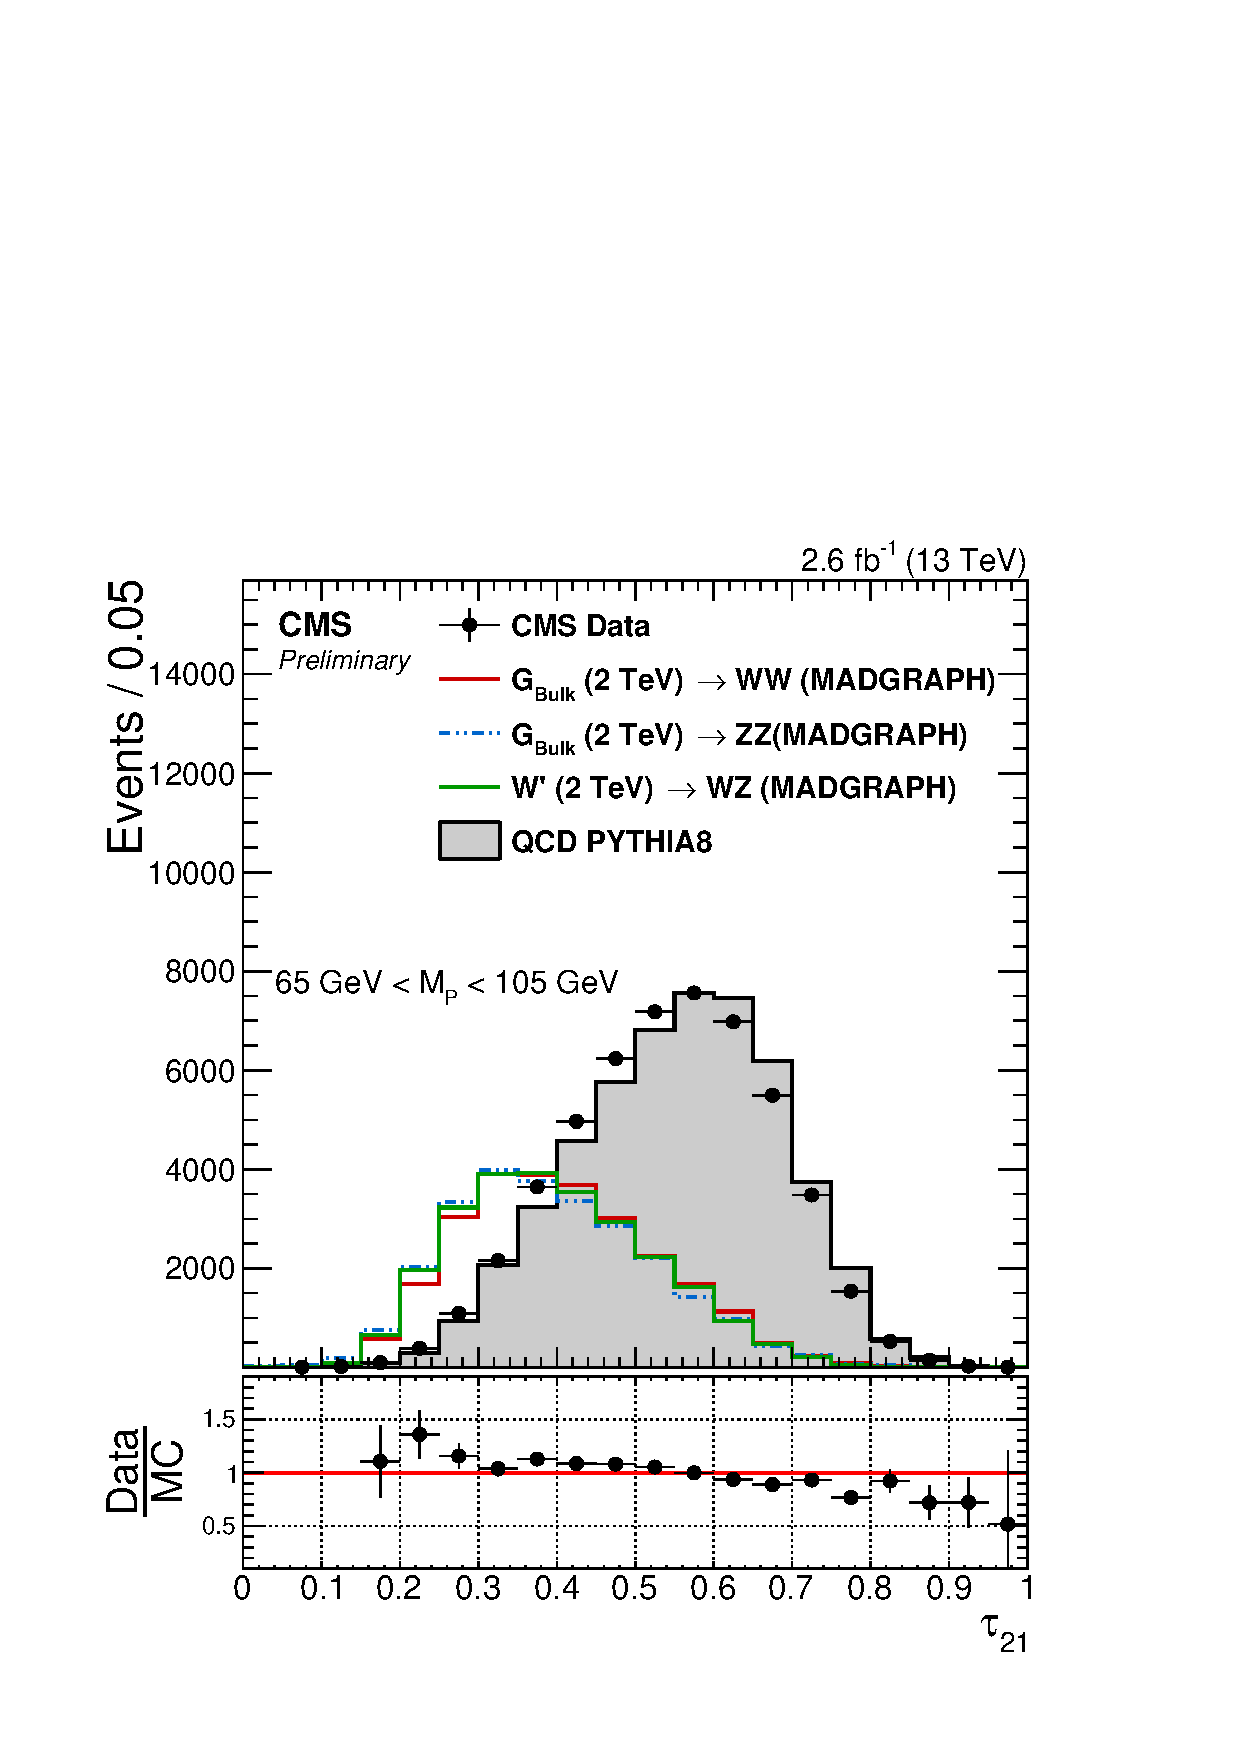
\includegraphics[width=0.4\textwidth]{figures/analysis/search1/AN-15-211/controlplots/silverjson/Tau21_punzi_WSignal.pdf}\\
\caption{Pruned jet mass (left) and $\tau_{21}$ (right) distributions for data and simulated samples. Simulated samples are scaled to match the distribution in data. The $\tau_{21}$ distribution is shown for jets after a cut on the pruned jet mass of $65 {\GeV} < m_{p} < 105 {\GeV}$ has been applied.}
\label{fig:wtag}
\end{figure}

\subsection{Analysis categorization}
As the analysis requires two W/Z-tags, we always require one HP-tagged jet and then divide into LP and HP categories depending on whether the other jet is of high or low purity. In addition, in order to further enhance the analysis sensitivity, we further split the pruned jet mass window into a W and a Z boson window where the W window is defined as $65 {\GeV} < m_{p} < 85 {\GeV}$ and the Z boson window as $85 {\GeV} < m_{p} < 105 {\GeV}$. This has the added benefit of allowing us to discriminate between a \BulkG decaying to \WW or \ZZ, and a \PWpr decaying into \WZ by separating these events into categories. The signal yield will be higher in the WZ category for a \PWpr decaying to a W and Z boson than for a \BulkG decaying to \WW or \ZZ. Figure~\ref{fig:searchI:massCatWpr} shows the relative expected signal yield (left) and expected limits (left) in the different mass categories for a \PWpr with a mass of 2 TeV.
 \begin{figure}
 \centering
 \begin{minipage}{0.5\textwidth}
 \centering
 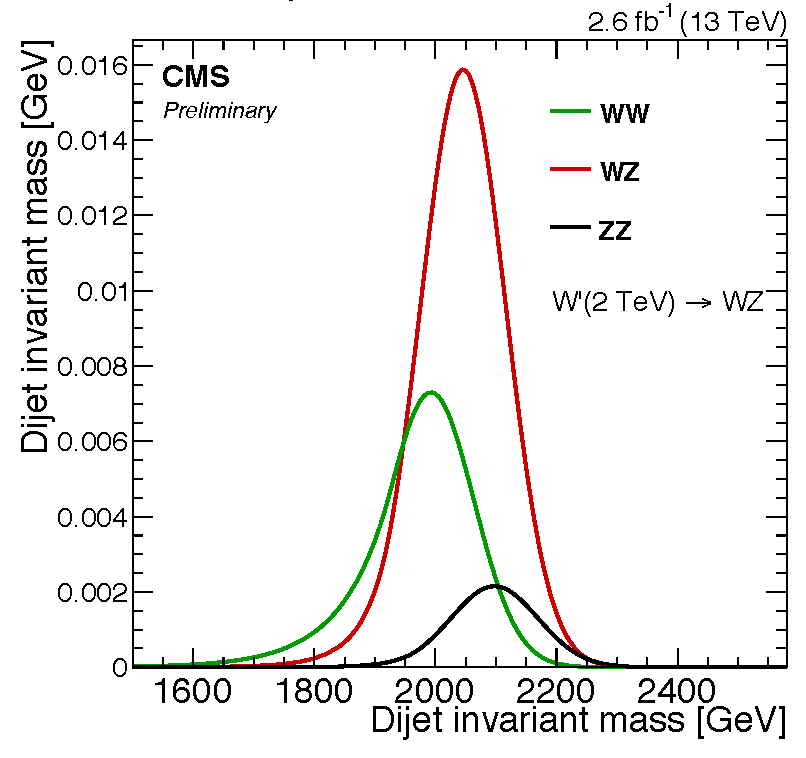
\includegraphics[width=0.99\textwidth]{figures/analysis/search1/misc/massCategories.pdf}
 \end{minipage}
 \begin{minipage}{0.29\textwidth}
 \centering
 \captionsetup{type=table} %% tell latex to change to table
 \begin{tabular}{| l | c |}
 \hline
 \multicolumn{2}{|c|}{$\PWpr (2 \TeV) \rightarrow \WZ$}\\
 \hline
 Category & Expected limit \\
 \hline
 WWHP & 2.1984 \\ 
 WWLP & 2.3261 \\ 
 WZHP & 1.2419 \\ 
 WZLP & 1.7157 \\ 
 ZZHP & 7.0855 \\ 
 ZZLP & 9.2012 \\ 
 \hline
 \end{tabular}
 \end{minipage}
 \caption{The expected signal yield per mass category for a \PWpr (2 \TeV) decaying to a \PW and a \PZ (left) together with the expected limit per mass category for the same signal (right).}
 \label{fig:searchI:massCatWpr}
 \end{figure}
All categories are combined in the end, leading to the same or better sensitivity at each resonance mass value than when using the whole pruned mass window. Figure~\ref{fig:searchI:massCategories} shows the expected 95\% CL upper limits on the production cross section of a \PWpr decaying to \WZ (left) and a \BulkG decaying to \WW (right) as a function of the resonance mass in the HP category. The blue line corresponds to the expected limits obtained when not splitting into mass categories and the red line corresponds to the limit using the combination of two categories. The dotted and solid black lines are the limits for the \PW and \PZ categories, respectively. The combination of two mass categories leads to slightly better (~10\%) or similar sensitivity as when using one large mass window.
\begin{figure}[h!]
 \centering
 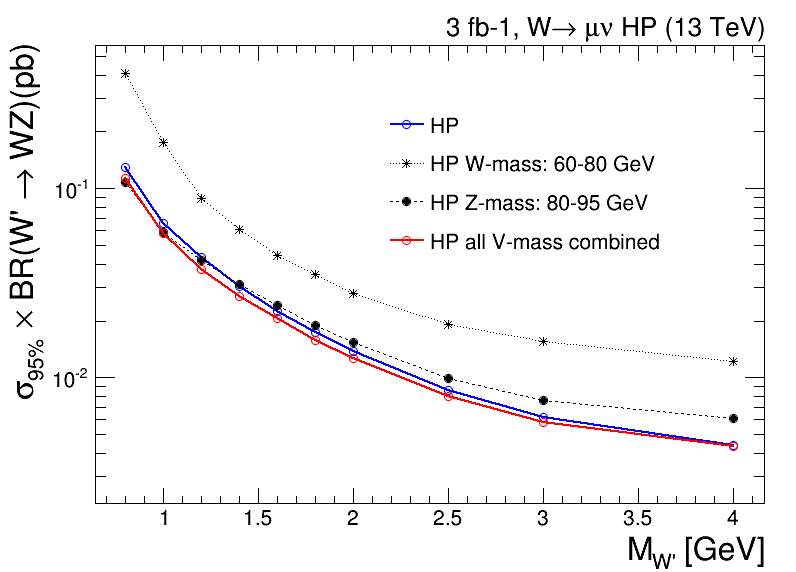
\includegraphics[width=0.49\textwidth]{figures/analysis/search1/AN-15-196/massCategories/compare-HP-HPV-Wprime.png}
  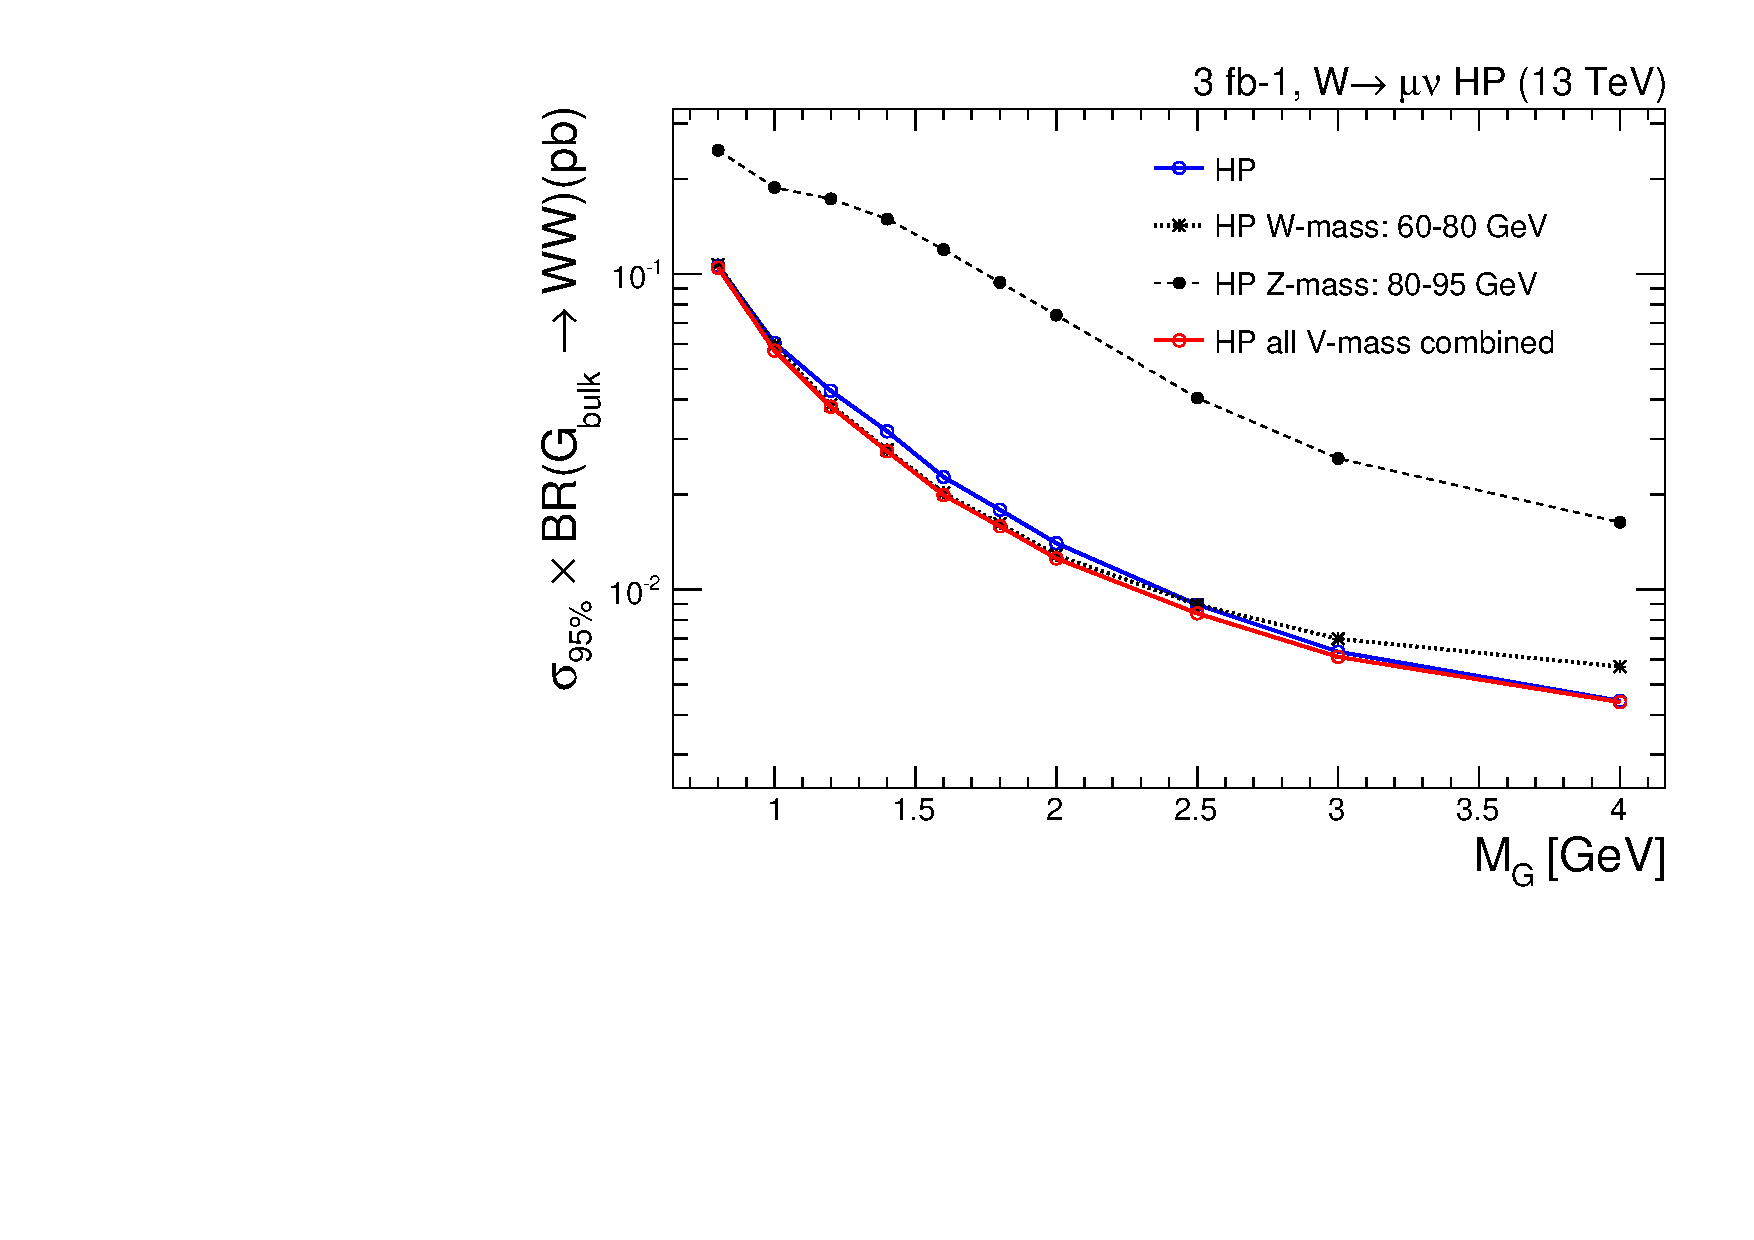
\includegraphics[width=0.49\textwidth]{figures/analysis/search1/AN-15-196/massCategories/compare-HP-HPV-BulkG.pdf}
 \caption{Expected 95\% CL upper limits on the production cross section of a \PWpr (left) and \BulkG (right) signal as a function of the resonance mass for the different mass categories for events passing the high-purity $\tau_{21}$ selection.}
 \label{fig:searchI:massCategories}
 \end{figure}
 The real benefit of splitting into mass categories becomes obvious when defining a test statistics based on the likelihood ratios of each signal hypothesis, $q = -2 \ln(L_{\BulkG}/L_{\PWpr})$, shown in Figure~\ref{fig:searchI:signalsep}. For a signal with a signal strength corresponding to a 3-4 $\sigma$ excess, the test statistics for each signal hypothesis are well separated ($\sim3.5 \sigma$), allowing us to make a statement of whether a possible signal is more likely due to a \BulkG or a \PWpr particle.
\begin{figure}[h!]
 \centering
 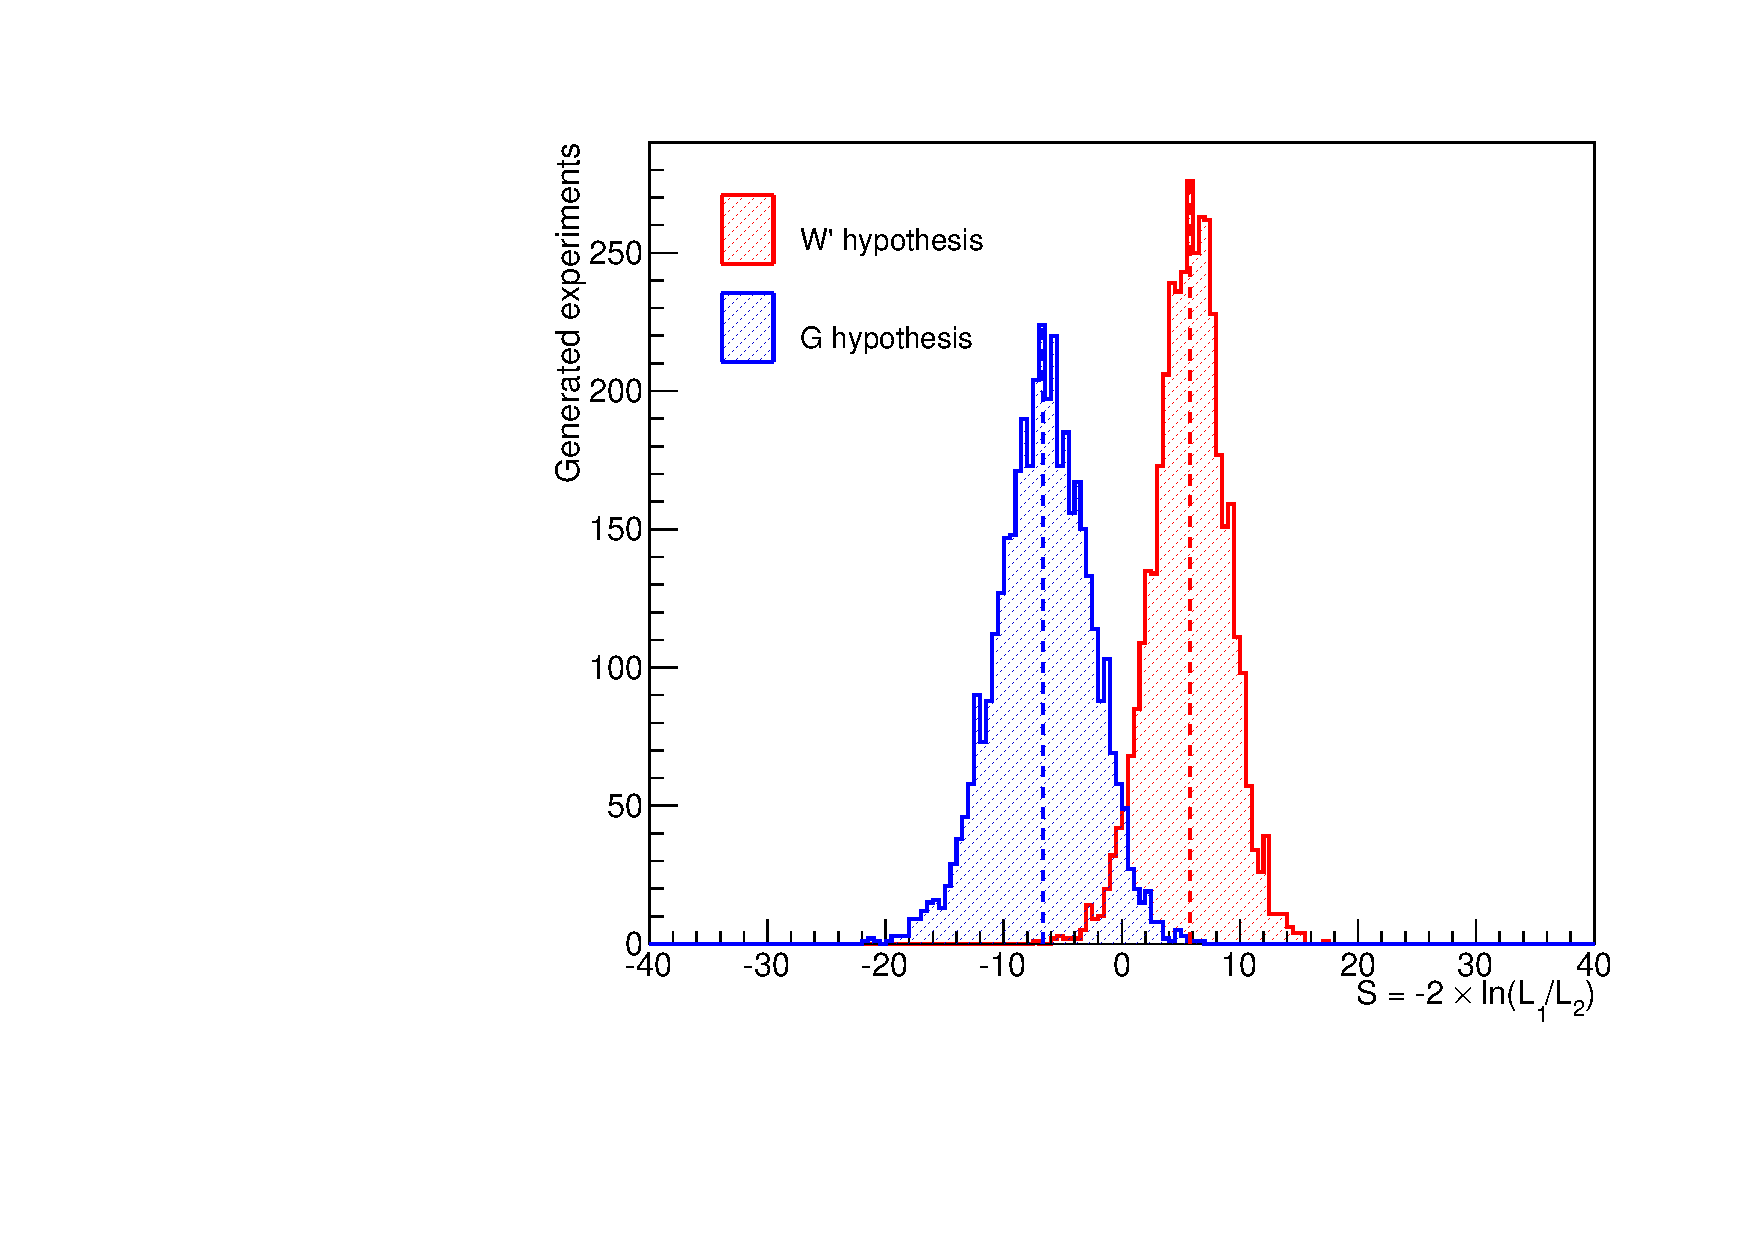
\includegraphics[width=0.49\textwidth]{figures/analysis/search1/AN-15-196/massCategories/sig_sep.pdf}
 \caption{Distribution of the test statistic  $q = -2 \ln(L_{\BulkG}/L_{\PWpr})$ for a \BulkG (blue) and \PWpr signal hypothesis.}
 \label{fig:searchI:signalsep}
 \end{figure}
With the high-purity and low-purity categories as defined above for each mass window combination, this leaves us with six different signal categories:  HP with 3 mass categories corresponding to WW, WZ, and ZZ, and the same 3 mass categories for LP. In parallel to the mass-category based analysis, we perform an analysis without categorization in mass (similar to the 8 \TeV analysis) as a cross-check. We found the sensitivity with mass categories to be higher and hence will not present these studies here. The final tagging efficiency for different signal hypotheses (top) together with the QCD mistag rate (bottom) in the different signal categories is shown in Figure~\ref{fig:search1:sigeff}. The solid lines represent the tagging efficiency in the full mass window ($65 {\GeV} < m_{p} < 105 {\GeV}$) before splitting into mass categories. A lower signal efficiency in the ZZ mass category is observed in all cases. This can be explained from the pruned jet mass distribution on the left in Figure~\ref{fig:wtag}, where a lower pruned jet mass selection of 85 GeV leaves a large fraction of the Z peak in the W mass window. The main benchmark models under consideration preferably decay to W bosons, since in the Bulk Graviton model the branching ratio BR($G_{Bulk}$ $\rightarrow$\WW) = 2* BR($G_{Bulk}$$\rightarrow$ \ZZ) and in the HVT model \PWpr/\PZpr$\rightarrow$ WZ/WW (but not \ZZ). Therefore, the tagging procedure is optimized for a high efficiency to tag W bosons. In the limit-setting procedure all the categories are combined and the overall signal efficiency is maintained. For the combined mass-categories (solid line) the signal efficiency is between 16 and 23\% in the double-tag categories, and between 20 and 34 \% in the single-V tag categories. The mistagging rate is below 1\% in the high-purity category.
\begin{figure}[h!]
\centering
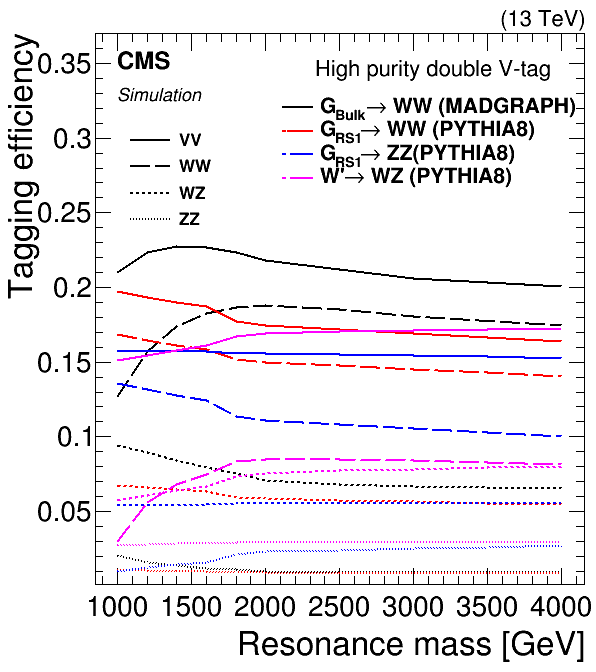
\includegraphics[width=0.49\textwidth]{figures/analysis/search1/AN-15-211/HP_VV_SigEff.png}
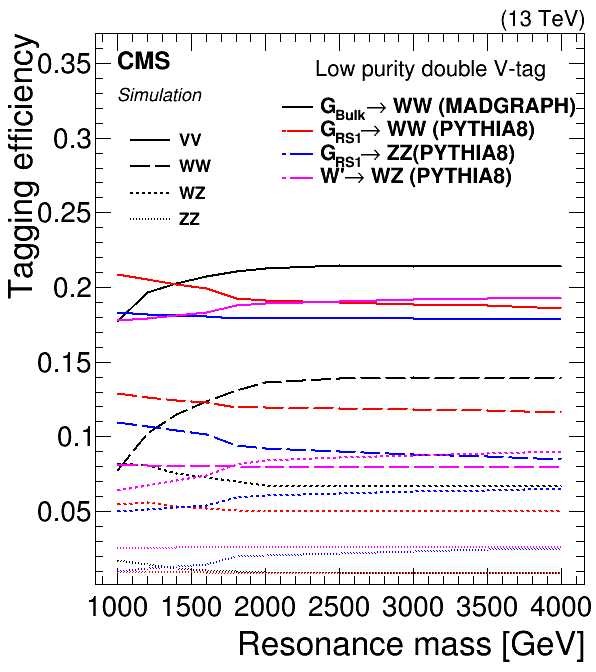
\includegraphics[width=0.49\textwidth]{figures/analysis/search1/AN-15-211/LP_VV_SigEff.png}\\
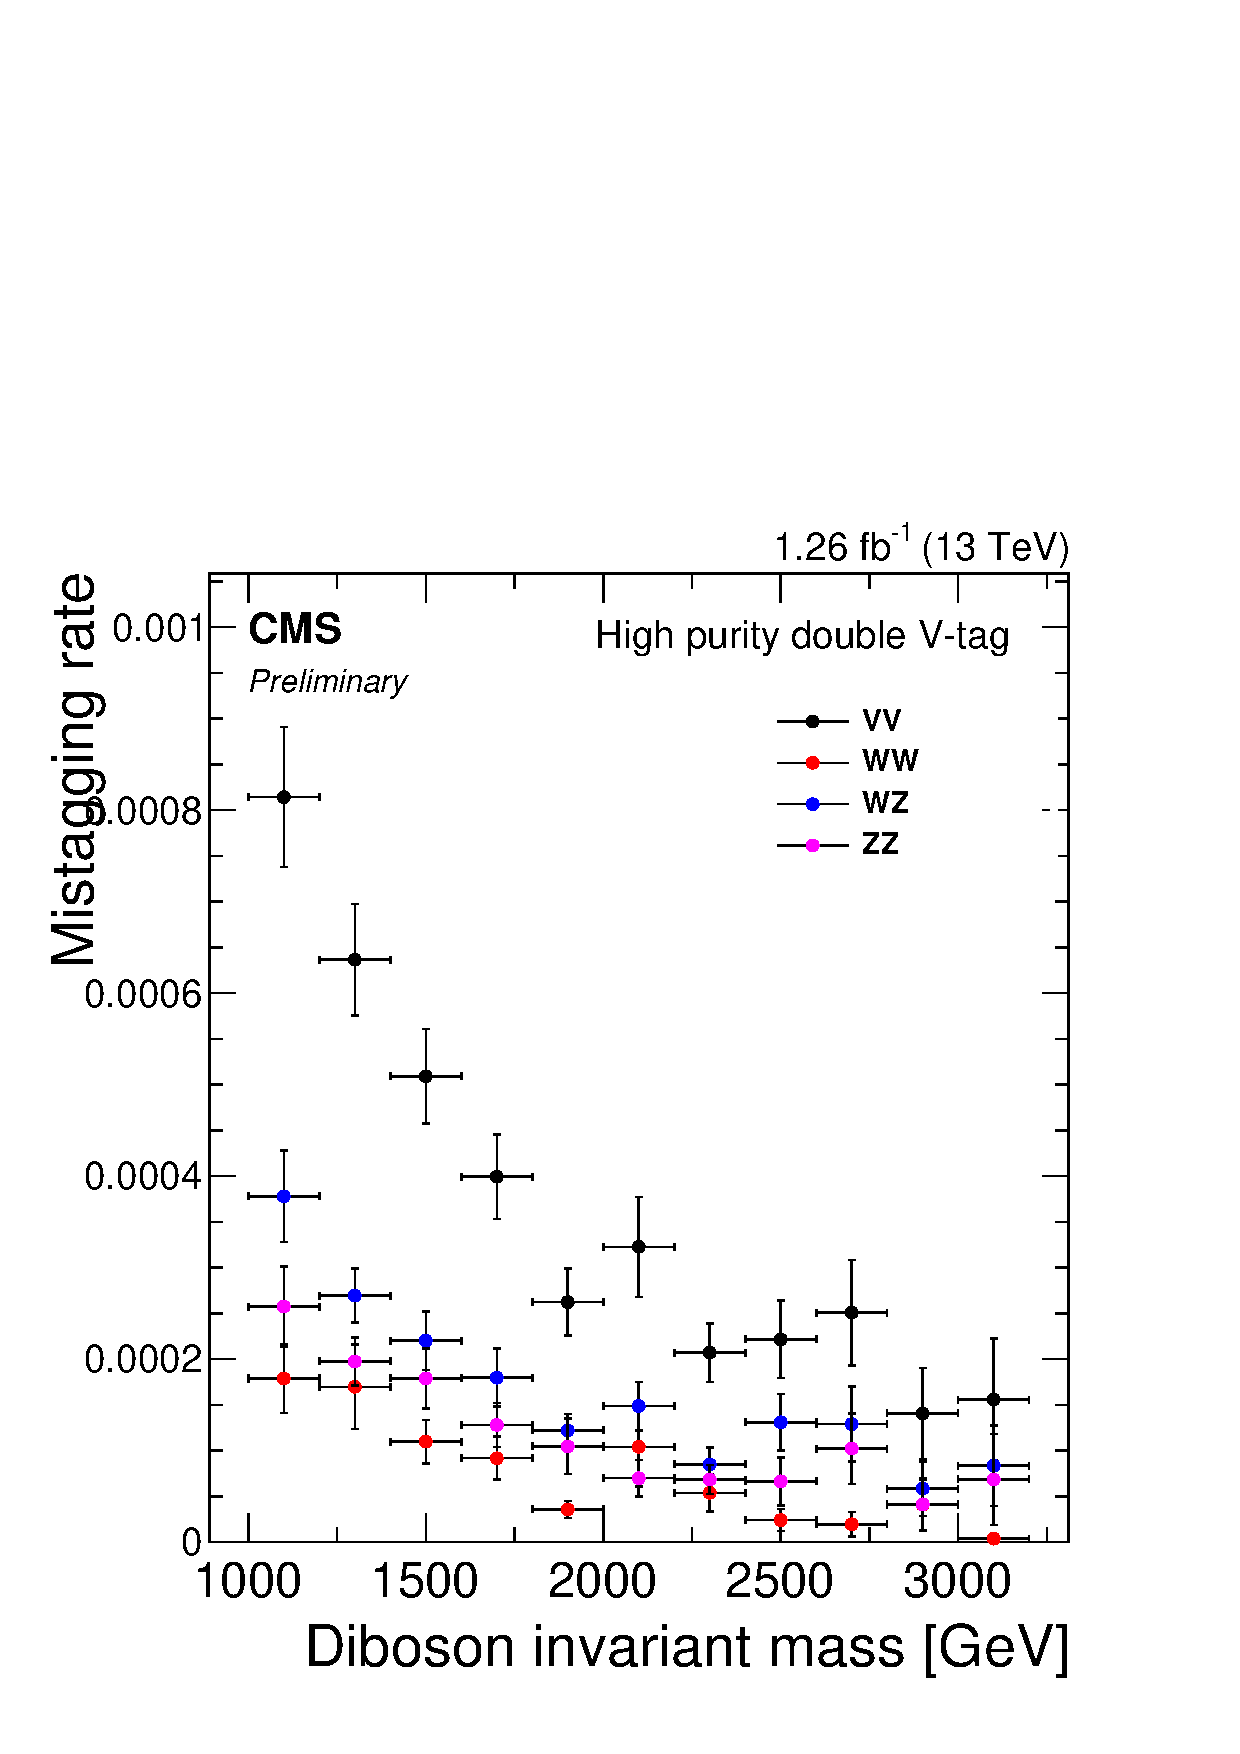
\includegraphics[width=0.49\textwidth]{figures/analysis/search1/AN-15-211/QCD_HP_VV_MistaggingRateEff.pdf}
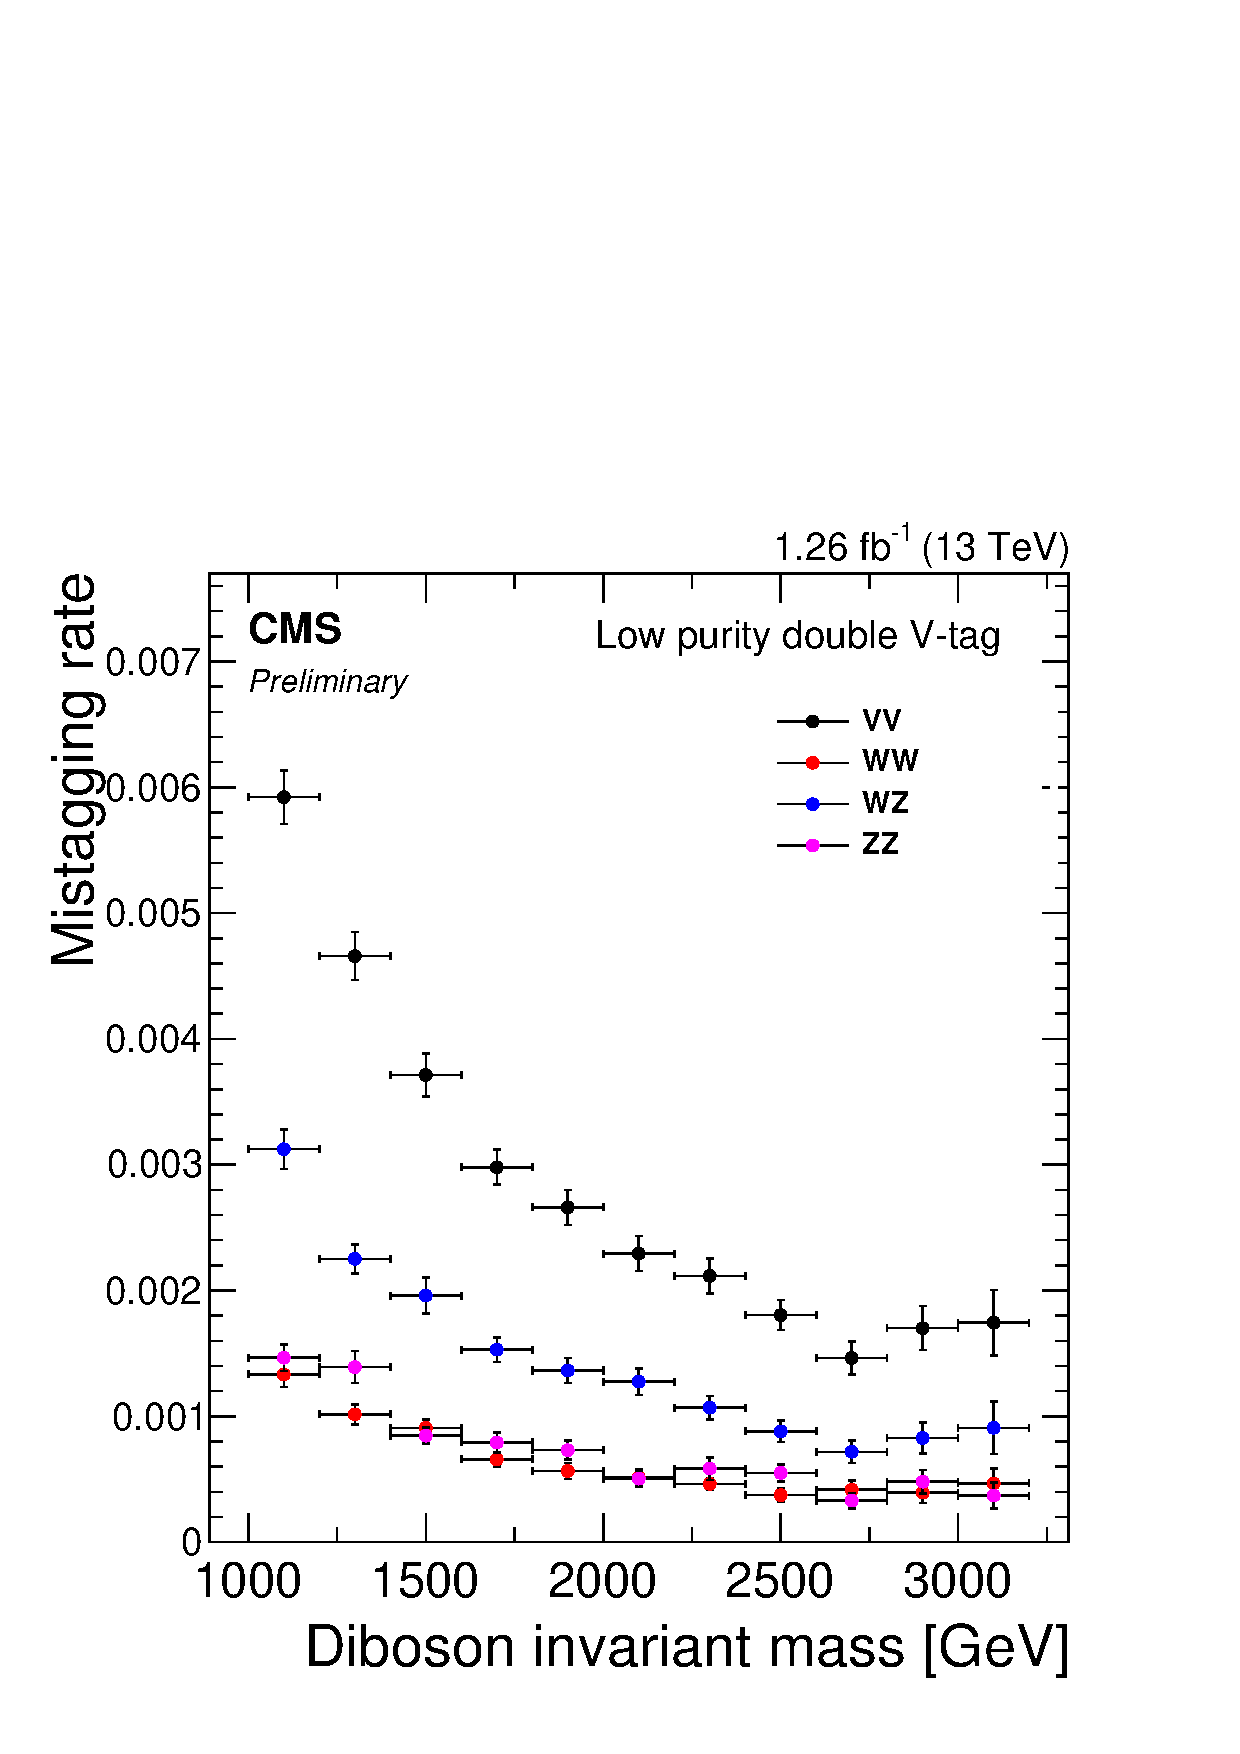
\includegraphics[width=0.49\textwidth]{figures/analysis/search1/AN-15-211/QCD_LP_VV_MistaggingRateEff.pdf}
\caption{Tagging efficiency (top) and mistagging rate (bottom) in the different pruned mass categories in the high-purity category (left) and in the low-purity category (right).}
\label{fig:search1:sigeff}
\end{figure}
The full analysis selections and final signal categories are listed in Table~\ref{tab:search1:selection}, where ${\mJ}_1$ and ${\mJ}_2$ refers to the jet with the highest and second highest jet \PT, respectively.
\begin{table}[!h!]
\footnotesize
\begin{center}
\renewcommand{\arraystretch}{1.2}
\begin{tabular}{lc}
\hline 
\multicolumn{1}{c}{Selection} & Value\\
\hline \hline
\multicolumn{1}{c}{Boson selections}\\
\cline{1-1}
V $\to\qqbar$ (2 AK8 jets) & $\pt >200\GeV$\\
  & $|\eta| < 2.4$\\
Pruned jet mass & $65 < {\mJ}_1,{\mJ}_2  < 105\GeV$\\
Topology    & $|\Delta \eta_\mathrm{jj}| < 1.3$\\
Dijet invariant mass     & $\mjj >1\TeV$\\ 
2- to 1-subjettiness ratio    & $\nsubj < 0.75$\\
\hline
%\hline
\multicolumn{1}{c}{\mJ{} categories}\\
\cline{1-1}
WW & $ 65 < {\mJ}_{1} < 85\GeV$, $ 65 < {\mJ}_{2} < 85\GeV$\\
WZ & $ 65 < {\mJ}_{1} < 85\GeV$, $ 85 < {\mJ}_{2} < 105\GeV$\\
ZZ & $ 85 < {\mJ}_{1} < 105\GeV$, $ 85 < {\mJ}_{2} < 105\GeV$\\
\hline
\multicolumn{1}{c}{\nsubj{} categories}\\
\cline{1-1}
High-purity   & $\tau_{\rm{21, jet1}} < 0.45$, $\tau_{\rm{21, jet2}} < 0.45$\\
Low-purity    & $\tau_{\rm{21, jet1}} < 0.45$, $0.45 < \tau_{\rm{21, jet2}} < 0.75$\\
\hline						       
\end{tabular}
\caption{The full analysis selections, and the signal categories based on the pruned jet mass and \nsubj values.}
\label{tab:search1:selection}
\end{center}
\end{table}
\clearpage

\section{Background modeling}
\label{sec:searchI:bkg}
We assume that the QCD multijets background can be described by a smooth, monotonically decreasing function, which is parametrizable. This is similar to what is done in previous CMS analyses looking for bumps in the dijet invariant mass spectrum~\cite{Chatrchyan:2012ypy,CMS-PAS-EXO-12-059}. The search is then performed by fitting the sum of the functions for background and signal to the dijet invariant mass spectrum in data. Neither data control regions nor simulated samples are used directly by this method. The background functions are of the following form:
\begin{equation}
\label{eq:dijet1}
\frac{dN}{d\mjj}= \frac{ P_0 } { (\mjj/\sqrt{s})^{P_2} }\quad\quad\quad{\rm and}
\quad\quad\quad\quad
\frac{dN}{d\mjj}= \frac{ P_0(1-\mjj/\sqrt{s})^{P_1} } { (\mjj/\sqrt{s})^{P_2} }\:\:,
\end{equation}
where $m$ is the dijet invariant mass, $\sqrt{s}$ is the center-of-mass energy, $P_0$ is a normalization parameter for the probability density function, and $P_1$ and $ P_2$ describe the shape. The number of fit parameters is decided through a Fisher's F-test~\cite{RePEc:bla:istatr:v:80:y:2012:i:3:p:491-491}. In this test, we start from the 2-parameter function and compare the goodness of fit ($\chi^2$ divided by degrees of freedom) when fitting the data signal region with a 2, 3, 4 and 5 parameter function. If the confidence level is less than 10\%, we add additional parameters to model the background distribution. The 4- and 5-parameter functions are
\begin{align}
\label{eq:dijet2}
\frac{dN}{d \mjj} &= \frac{ P_0(1-\mjj/\sqrt{s})^{P_1} } {(\mjj/\sqrt{s})^{P_2+P_3\times\log(\mjj/\sqrt{s})} }\quad{\rm and}\\
\frac{dN}{d \mjj} &= \frac{ P_0(1-\mjj/\sqrt{s})^{P_1} } {(\mjj/\sqrt{s})^{P_2+P_3\times\log(\mjj/\sqrt{s})+P_4\times\log(\mjj/\sqrt{s})^2} },
\end{align}
where $P_3$ and $P_4$ are additional free parameters. As an additional crosscheck, an alternative fit function is also tested:
\begin{equation}
\label{eq:dijet4}
\frac{dN}{d\mjj} = \frac{ P_0(1-\mjj / \sqrt{s}+P_3(\mjj / \sqrt{s})^2)^{P_1} } { (\mjj/\sqrt{s})^{P_2} }.
\end{equation}
The fit range is chosen such that it starts where the trigger efficiency has reached its plateau to avoid bias from trigger inefficiency, and extends to the bin after the highest $m_{VV}$ mass point. The binning chosen for the fit follows the detector resolution as in Refs.~\cite{Chatrchyan:2012ypy,CMS-PAS-EXO-12-059}. Before unblinding the signal region, we check that the QCD dijet invariant mass spectrum is expected to be smooth from the distribution in QCD MC as well as exercise the F-test in QCD MC and in a data sideband.\par
The fits to data in the signal region using the different fit functions are shown in Figure \ref{fig:searchI:fit-dataVV}, and the corresponding F-test output are given in Tables~\ref{tab:WW_enriched} through~\ref{tab:ZZ_enriched}. The findings can be summarized as follows: for the WW enriched category, a 2-parameter fit is sufficient to describe the data in both the high- and low-purity categories. In the WZ category, a 2-parameter fit is sufficient in the high-purity category, while three parameters are needed for the low-purity category. For the ZZ category, a 3-parameter fit is needed for both purity categories. The 2- and 3-parameter fit functions as defined in Equation \ref{eq:dijet2} will therefore be used to model the background component in the simultaneous signal and background fit.
\begin{figure}[h!]
\centering
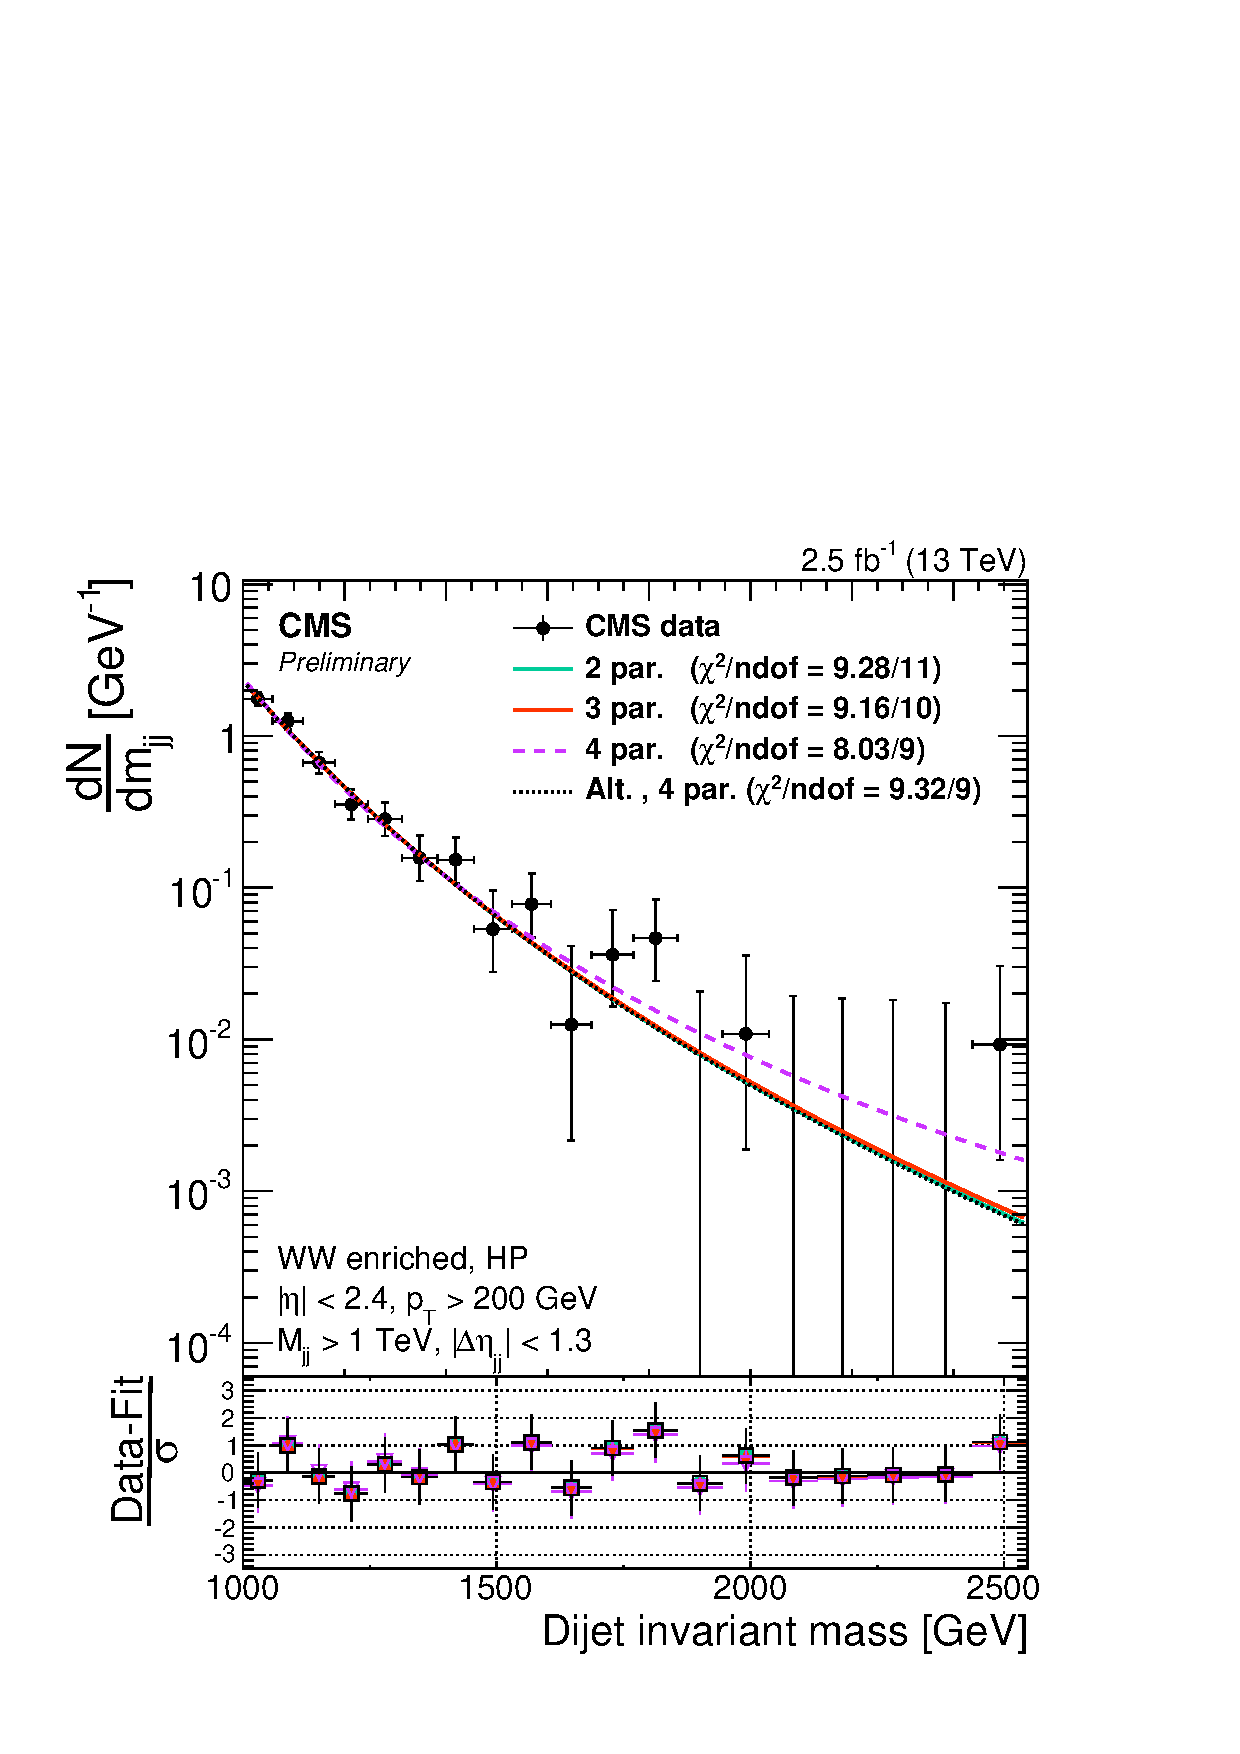
\includegraphics[width=0.32\textwidth]{figures/analysis/search1/AN-15-211/ftest/no5par/WWHP_fitComp.pdf}
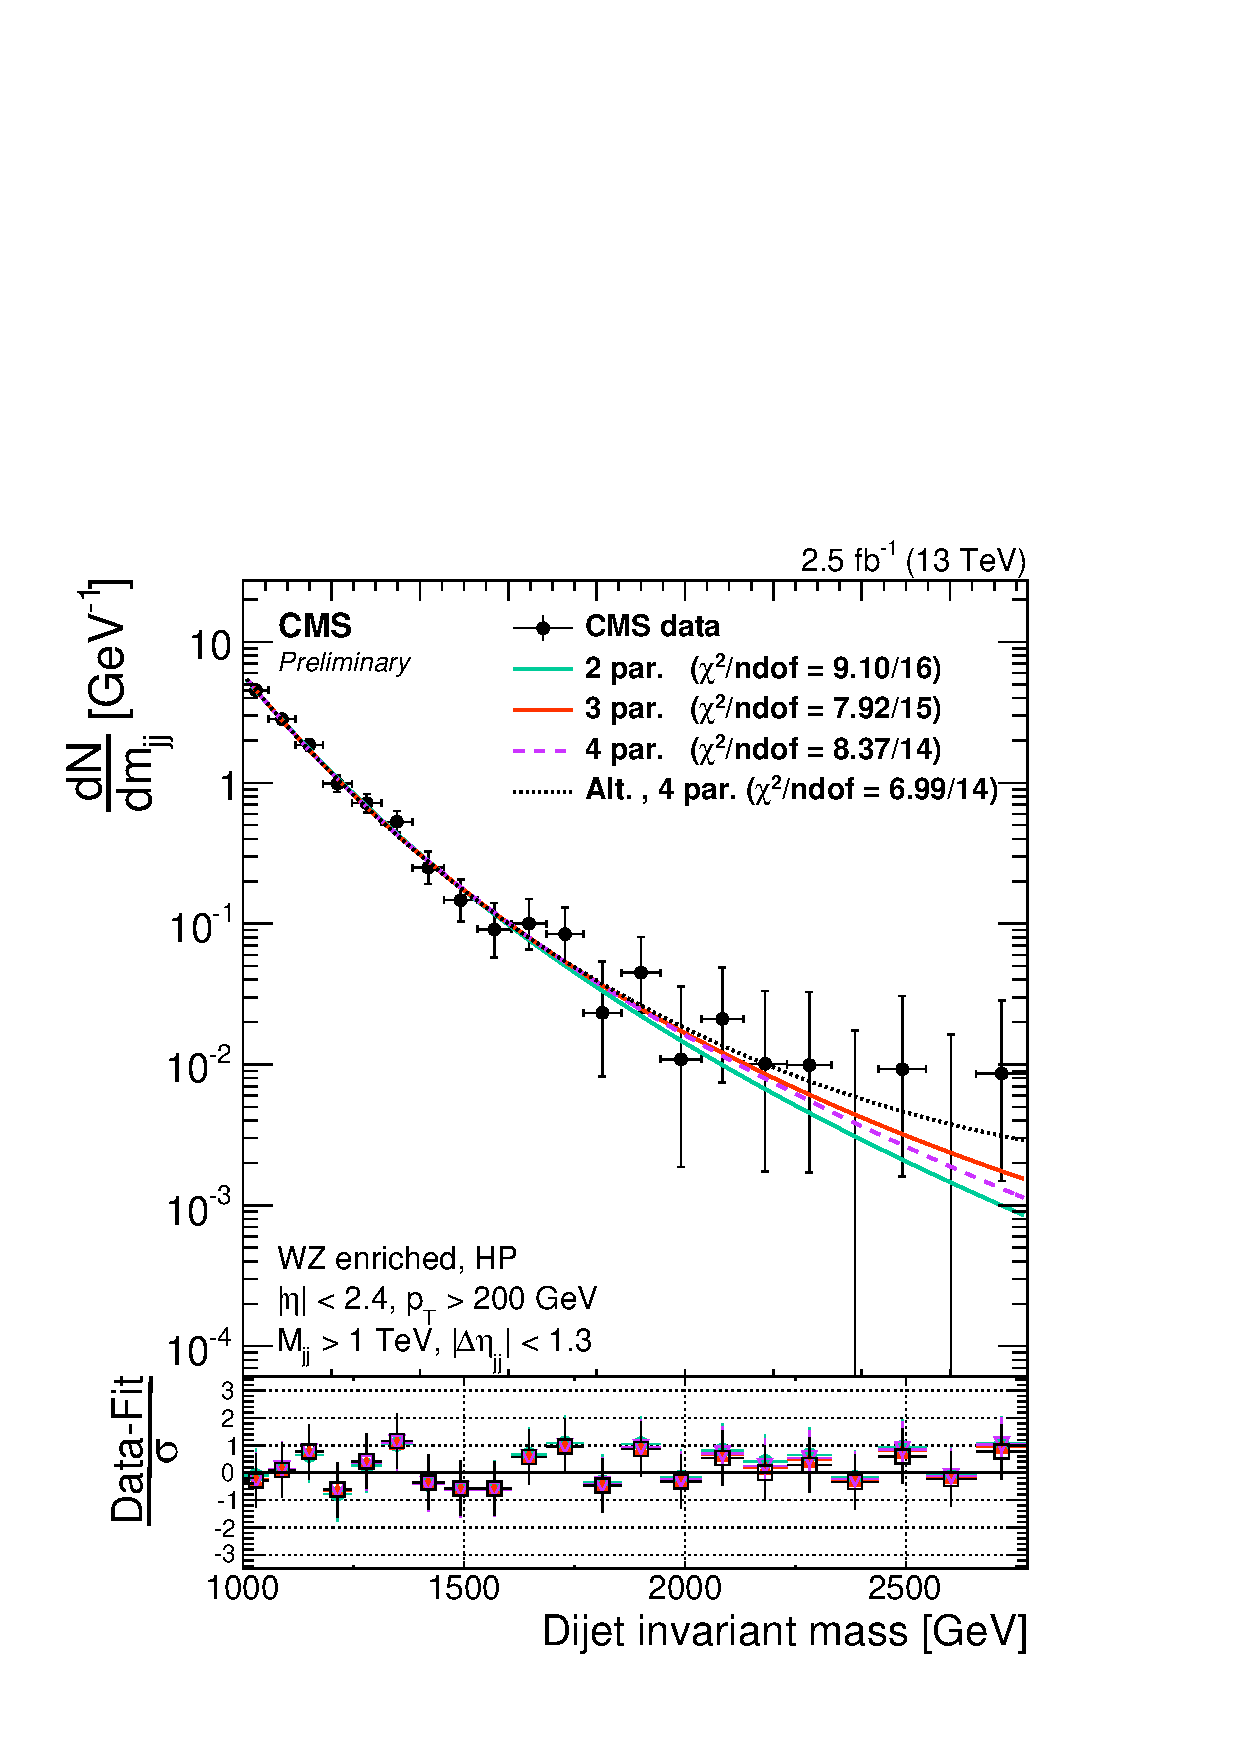
\includegraphics[width=0.32\textwidth]{figures/analysis/search1/AN-15-211/ftest/no5par/WZHP_fitComp.pdf}
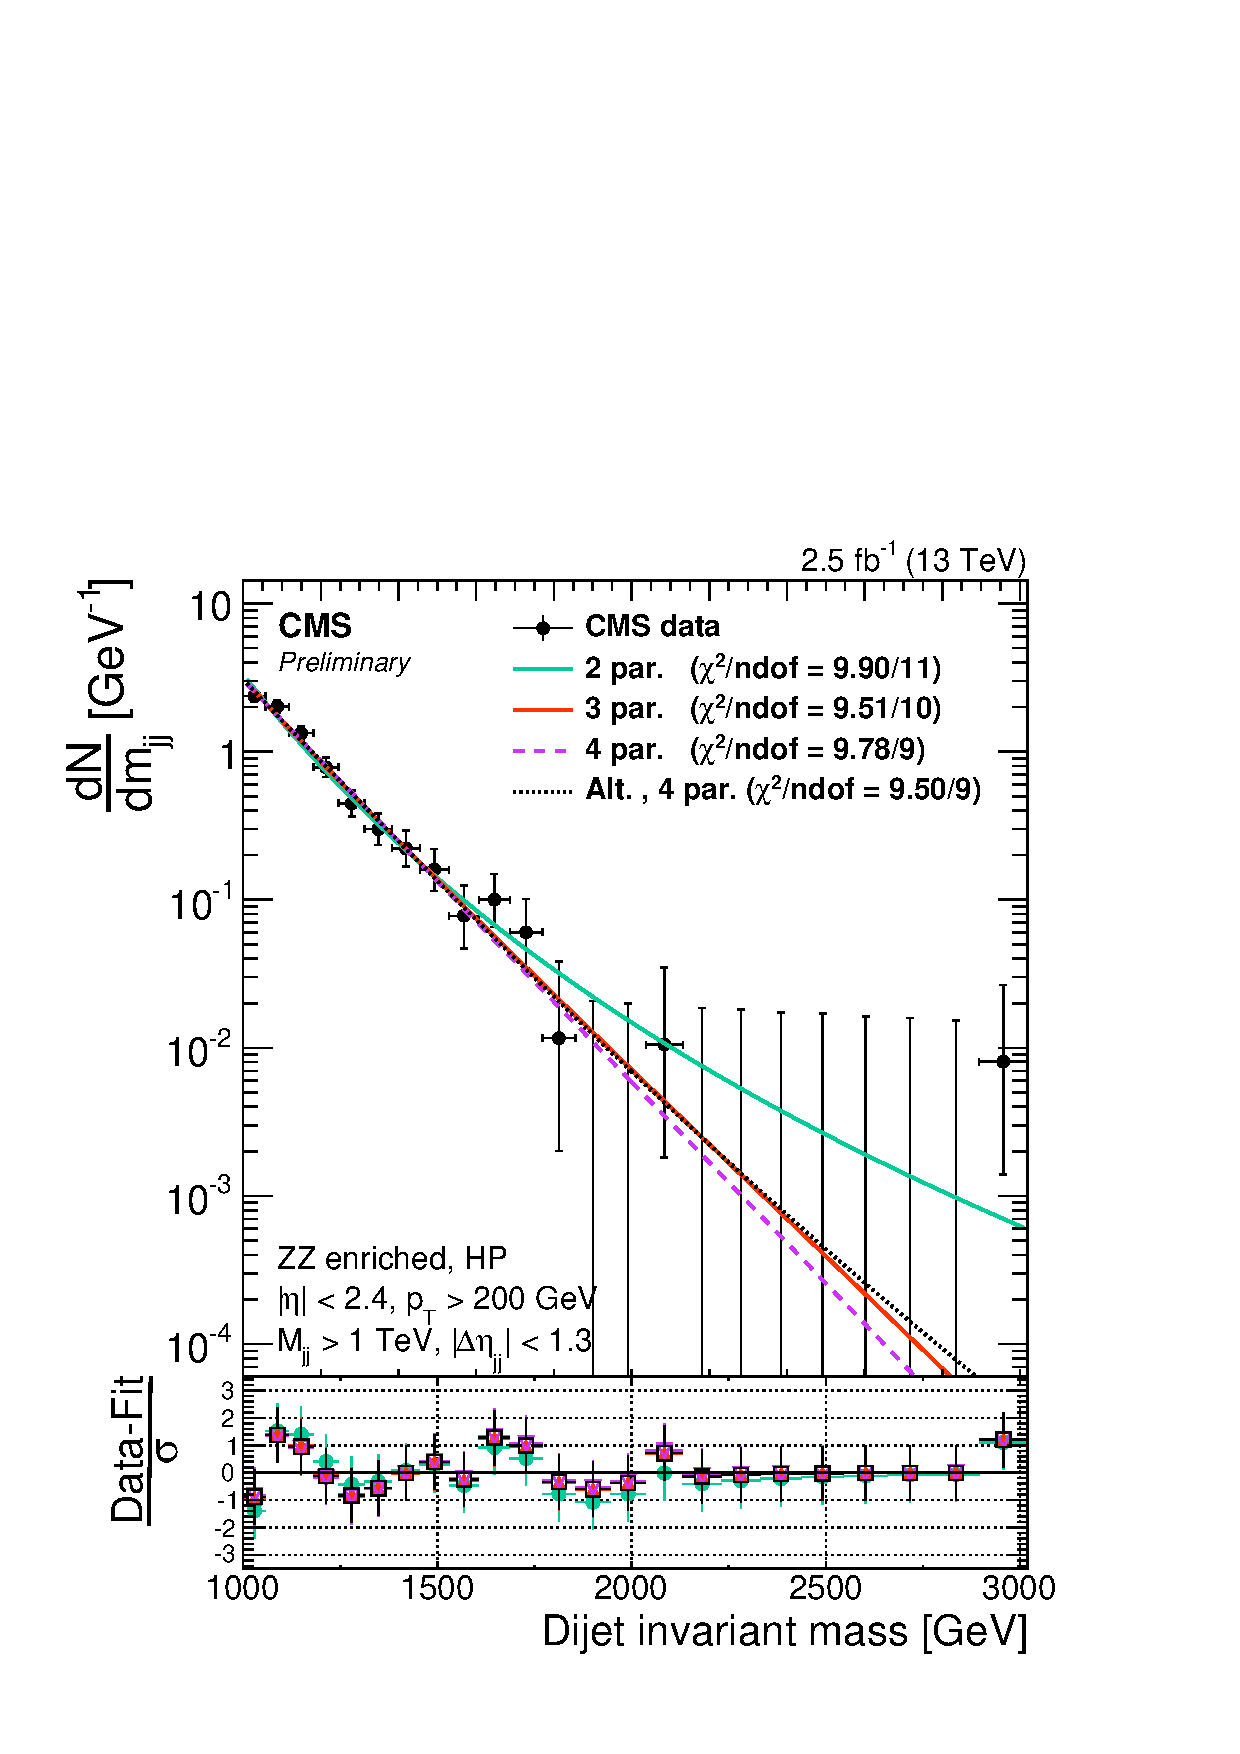
\includegraphics[width=0.32\textwidth]{figures/analysis/search1/AN-15-211/ftest/no5par/ZZHP_fitComp.pdf}\\
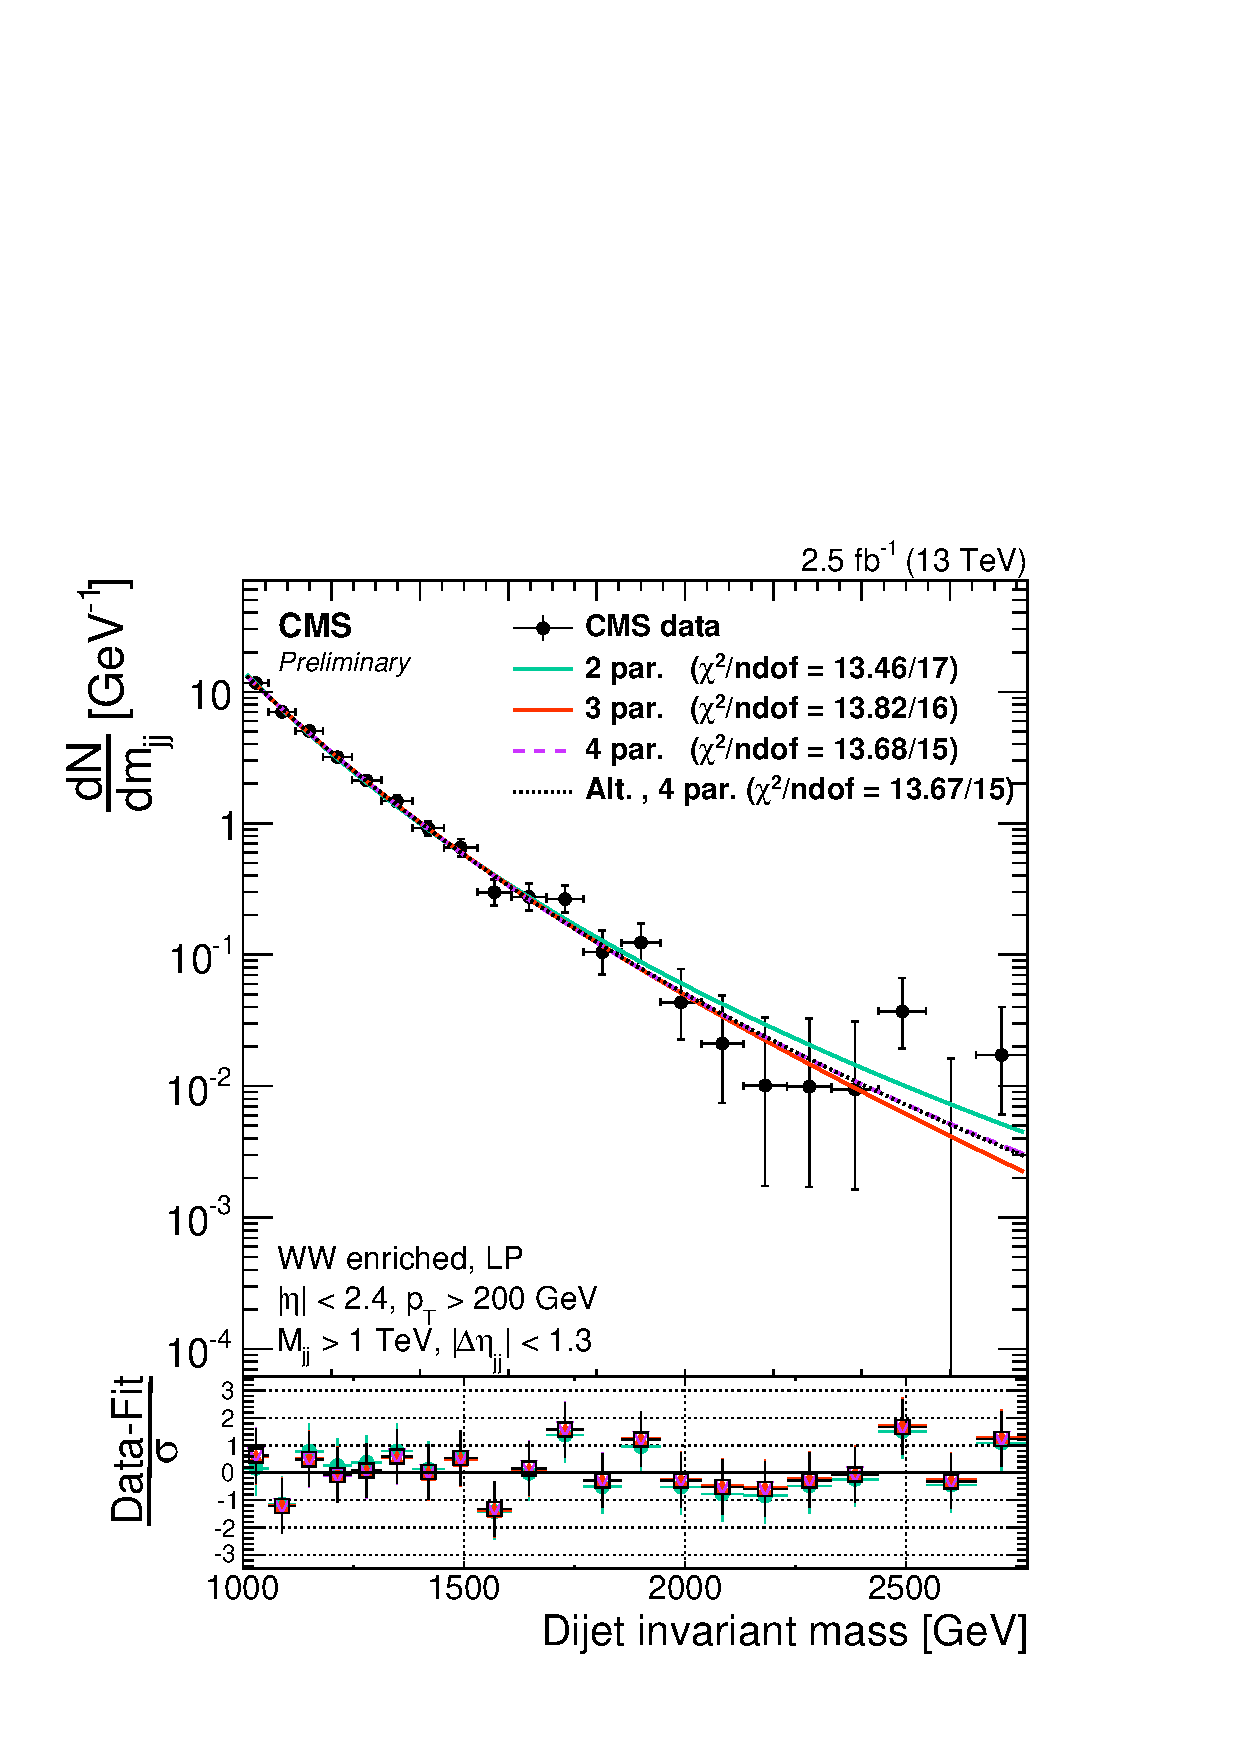
\includegraphics[width=0.32\textwidth]{figures/analysis/search1/AN-15-211/ftest/no5par/WWLP_fitComp.pdf}
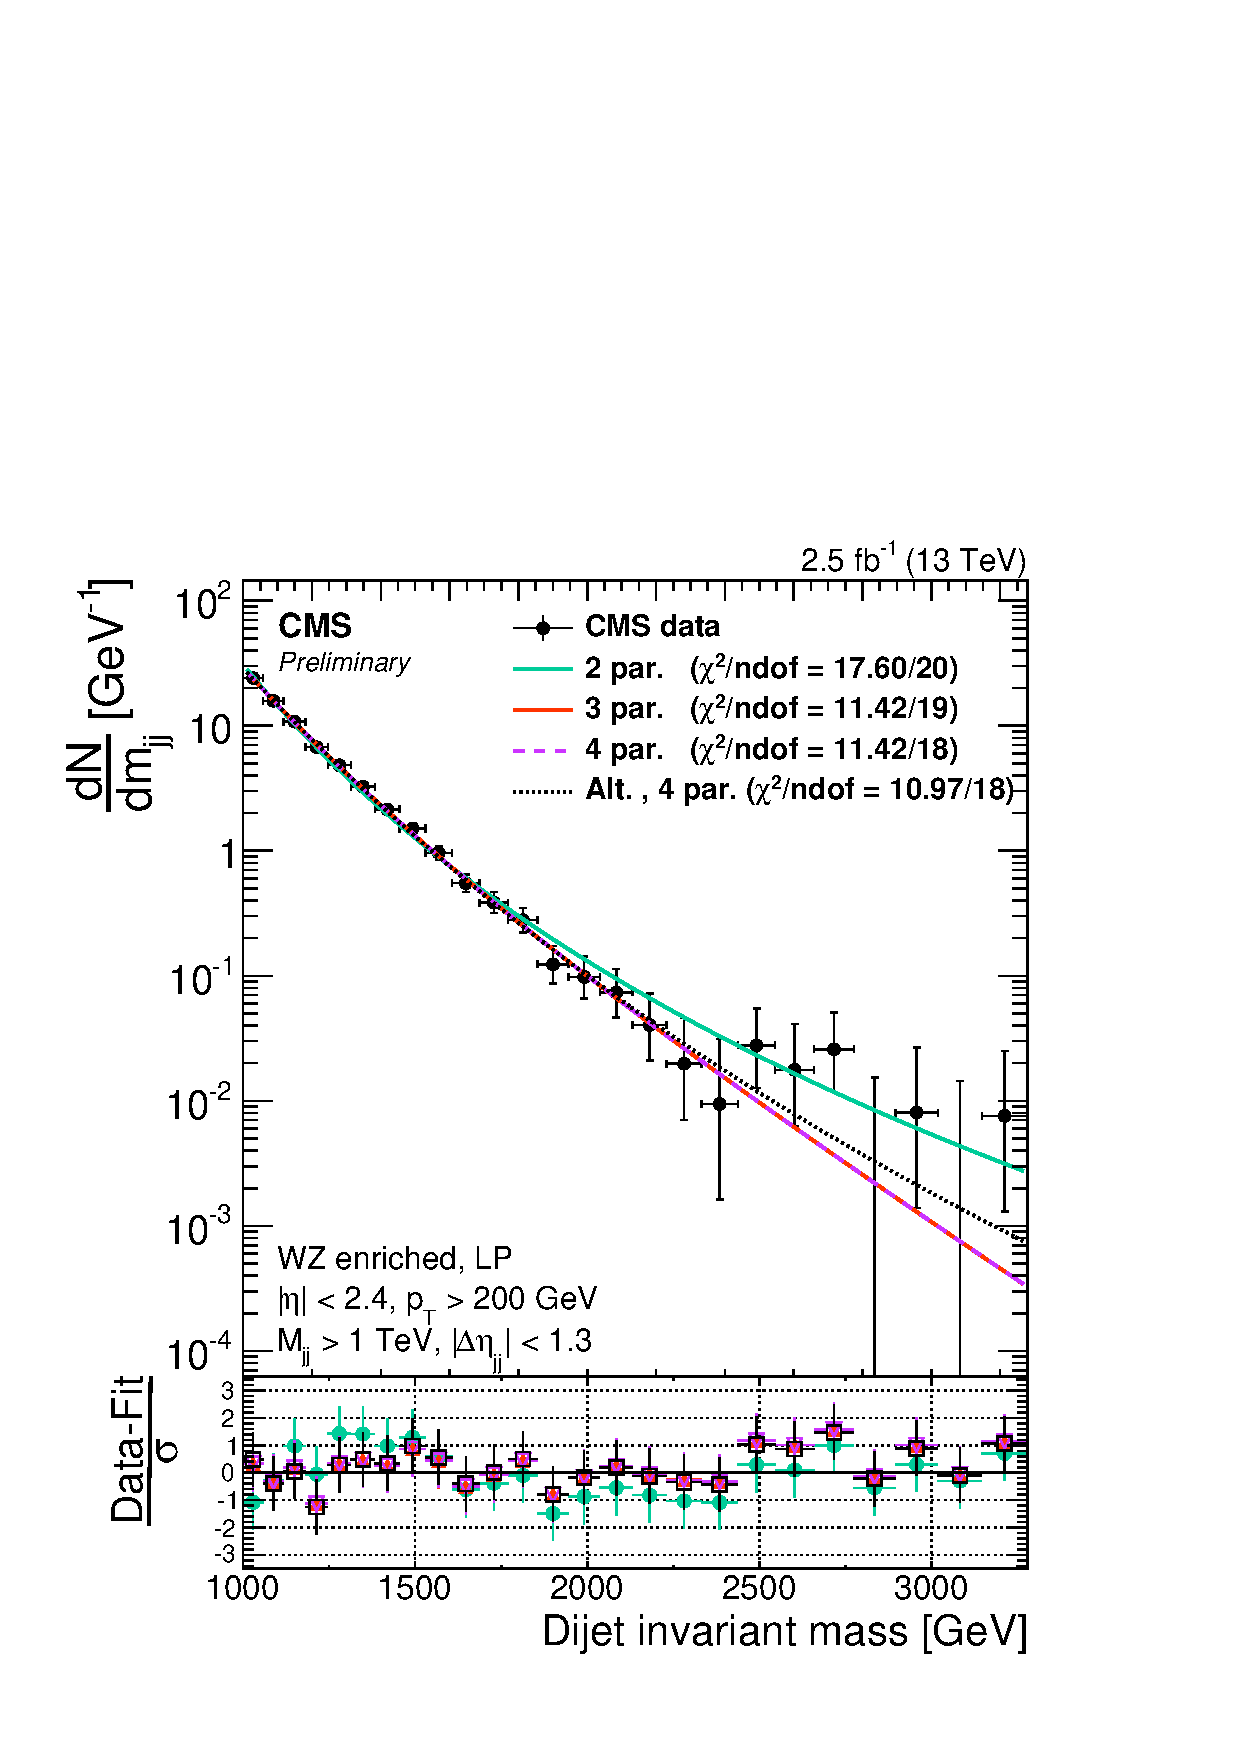
\includegraphics[width=0.32\textwidth]{figures/analysis/search1/AN-15-211/ftest/no5par/WZLP_fitComp.pdf}
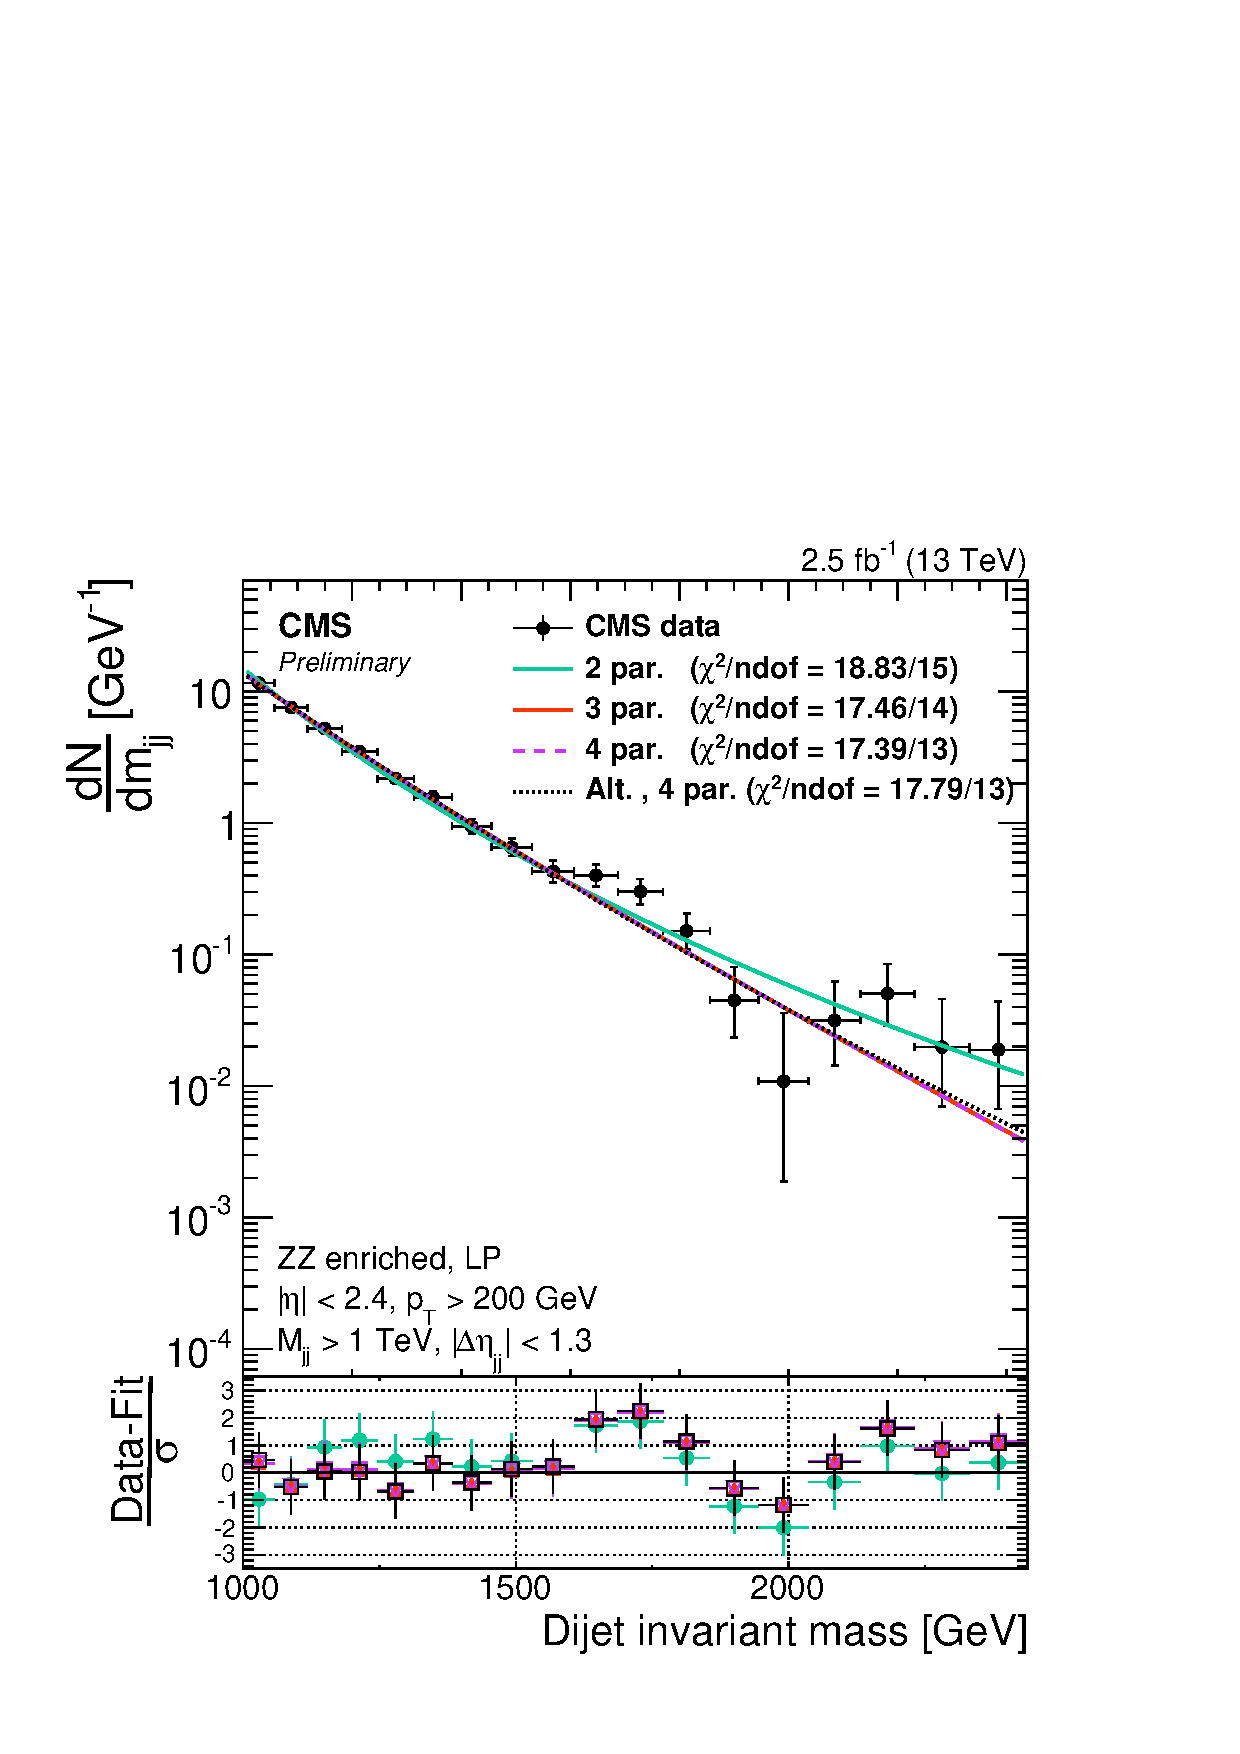
\includegraphics[width=0.32\textwidth]{figures/analysis/search1/AN-15-211/ftest/no5par/ZZLP_fitComp.pdf}
\caption{Fitted dijet mass spectrum in the different mass and purity categories in data. A 2-parameter fit is sufficient to describe the data in the WW- (HP and LP) and WZ-enriched (LP) categories. For the ZZ- (HP and LP) and WZ-enriched (HP) categories, a 3-parameter fit is needed.}
\label{fig:searchI:fit-dataVV}
\end{figure}
\begin{table}[h!]
\centering
\begin{tabular}{|l c c c |}
\hline
\multicolumn{4}{|c|}{WW-enriched, HP}\\
\hline
Function & Residuals & $\chi^2$ & ndof \\
\hline
2 par & 0.034 & 9.279 & 11 \\
3 par & 0.034 & 9.160 & 10 \\
4 par & 0.040 & 8.030 & 9 \\
\hline
\hline
Fishers23  & -0.053 &CL &1.0\\
Fishers34  & -1.456 &CL &1.0\\
\hline
\end{tabular}
\quad
\begin{tabular}{|l c c c |}
\hline
\multicolumn{4}{|c|}{WW-enriched, LP}\\
\hline
Function & Residuals & $\chi^2$ & ndof \\
\hline
2 par & 0.270 & 13.462 & 17 \\
3 par & 0.300 & 13.819 & 16 \\
4 par & 0.324 & 13.680 & 15 \\
\hline
\hline
Fishers23 & -1.723& CL & 1.0\\
Fishers34 & -1.191& CL & 1.0\\
\hline
\end{tabular}
\caption{Residuals, $\chi^{2}$, and degrees of freedom for the WW-enriched HP and LP categories. A 2-parameter fit is needed to describe the data in both categories.}
\label{tab:WW_enriched}
\end{table}
\begin{table}[h!]
\centering
\begin{tabular}{|l c c c |}
\hline
\multicolumn{4}{|c|}{WZ-enriched, HP}\\
\hline
Function & Residuals & $\chi^2$ & ndof \\
\hline
2 par & 0.039 & 9.105 & 16 \\
3 par & 0.047 & 7.915 & 15 \\
4 par & 0.048 & 8.370 & 14 \\
\hline
\hline
Fishers23 & -2.598& CL & 1.0\\
Fishers34 & -0.491& CL & 1.0\\
\hline
\end{tabular}
\quad
\begin{tabular}{|l c c c |}
\hline
\multicolumn{4}{|c|}{WZ-enriched, LP}\\
\hline
Function & Residuals & $\chi^2$ & ndof \\
\hline
2 par & 1.016 & 17.602 & 20 \\
3 par & 0.270 & 11.424 & 19 \\
4 par & 0.269 & 11.421 & 18 \\
\hline
\hline
Fishers23 & 55.258& CL & 0.0\\
Fishers34 & 0.078& CL & 0.783\\
\hline
\end{tabular}
\caption{Residuals, $\chi^{2}$, and degrees of freedom for the WZ-enriched HP (left) and LP (right) categories. A 2-parameter fit is sufficient to describe the data in the high-purity category, while three parameters are needed for the low-purity category.}
\label{tab:WZ_enriched}
\end{table}
\begin{table}[h!]
\centering
\begin{tabular}{|l c c c |}
\hline
\multicolumn{4}{|c|}{ZZ-enriched, HP}\\
\hline
Function & Residuals & $\chi^2$ & ndof \\
\hline
2 par & 0.220 & 9.901 & 11 \\
3 par & 0.140 & 9.511 & 10 \\
4 par & 0.124 & 9.781 & 9 \\
\hline
\hline
Fishers23 & 6.302& CL & 0.029\\
Fishers34 & 1.246& CL & 0.290\\
\hline
\end{tabular}
\quad
\begin{tabular}{|l c c c |}
\hline
\multicolumn{4}{|c|}{ZZ-enriched, LP}\\
\hline
Function & Residuals & $\chi^2$ & ndof \\
\hline
2 par & 0.448 & 18.832 & 15 \\
3 par & 0.121 & 17.463 & 14 \\
4 par & 0.118 & 17.394 & 13 \\
\hline
\hline
Fishers23 & 40.438& CL & 0.0\\
Fishers34 & 0.356& CL & 0.56\\
\hline
\end{tabular}
\caption{Residuals, $\chi^{2}$, and degrees of freedom for the ZZ-enriched LP and HP categories. A 3-parameter fit is sufficient to describe the data in both categories.}
\label{tab:ZZ_enriched}
\end{table}

\clearpage
\section{Signal modeling}
\label{sec:searchI:sig}

The signal shape is extracted from signal MC with resonance masses in the range from 1 to 4 TeV. A linear interpolation provides shapes for the mass points in between in steps of 100 GeV. From these shapes, signal shape models are constructed as composite models with a Gaussian core due to detector resolution and an exponential tail to account for parton distribution function effects. Parametric shape uncertainties due to jet energy scale and resolution uncertainties are inserted by variations of the Gaussian peak position and width. The dijet invariant mass shape for different benchmark model signals is shown in Figure \ref{fig:searchI:sigfit}. The signal and background components are then simultaneously fitted to the data points.
\begin{figure}[h!]
\centering
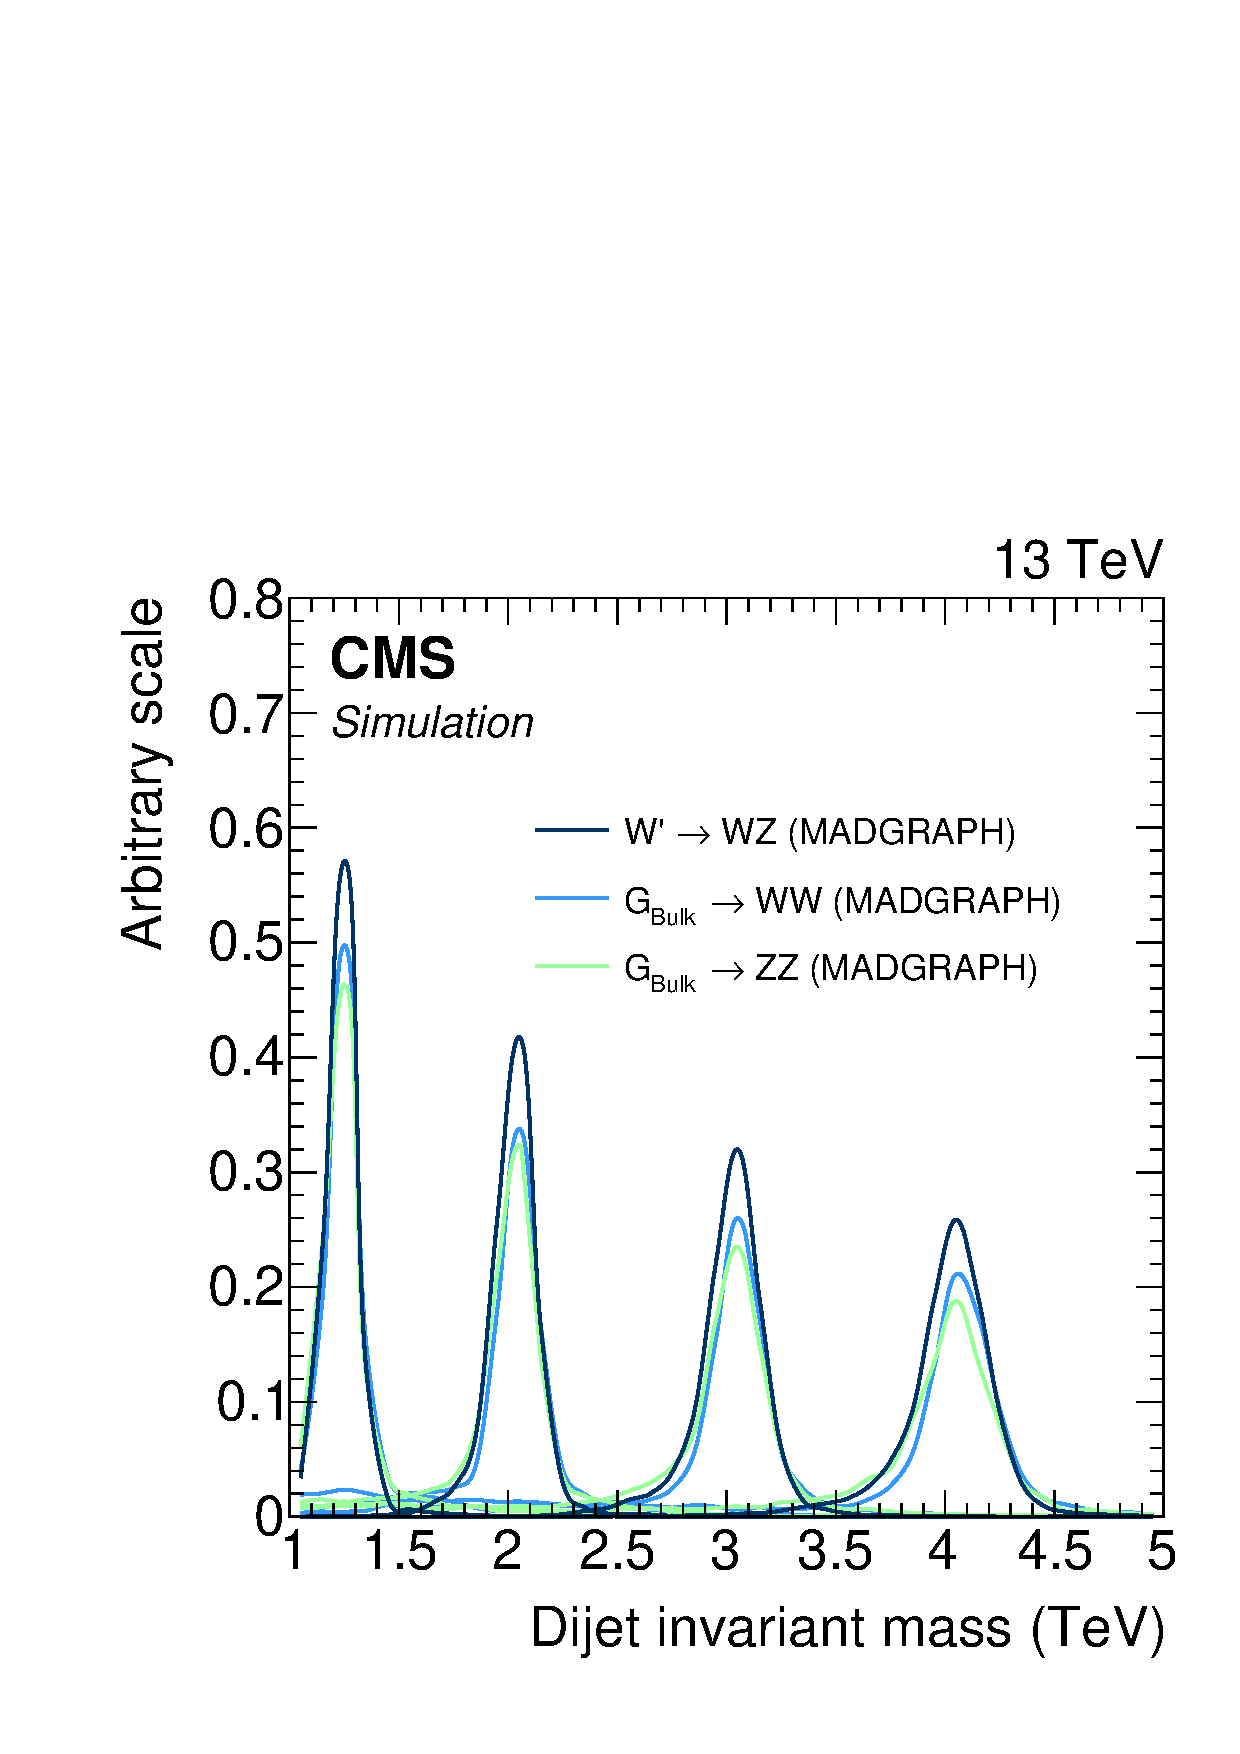
\includegraphics[width=0.49\textwidth]{figures/analysis/search1/B2G-16-004/Figure_005-a.pdf}
\caption{Dijet invariant mass from signal MC used to extract the signal shape, shown here for resonances with masses of 1.2, 2, 3, and 4 TeV.}
\label{fig:searchI:sigfit}
\end{figure}
\clearpage

\section{V-tagging scale factors}
\label{sec:searchI:vtag}
As seen in Figure~\label{fig:wtag}, some discrepancy is observed in the \nsubj distribution between data and MC. This can lead to a bias in the signal efficiency estimation and we therefore measure the real data signal efficiency in an orthogonal data sample.
The W-tagging efficiency is measured using real boosted \PW-jets in a semi-leptonic $\textrm{t}\bar{\textrm{t}}$ enriched data sample. This region is mainly quark-enriched, as opposed to the QCD gluon-enriched region we saw previously, and substructure variables are better described here. The sample is obtained through requiring a final state compatible with two b-jets and two \PW bosons, where one of the bosons decay leptonically and the other one hadronically. There are several good reasons to use this channel: Top quark pair production events are plentifully produced at the LHC, we can ensure a high purity of the sample through high-energy lepton, b-tag and missing energy requirements and lastly we can ensure that the \PW jets are boosted by requiring the leptonic leg, together with the hadronic \PW candidate, to have high transverse momentum. The final state is illustrated in Figure~\ref{fig:search2:ttsemilep}, with the object of interest being the AK R=0.8 jet containing the two quark daughters of the hadronically decaying \PW.
\begin{figure}[h!]
\centering
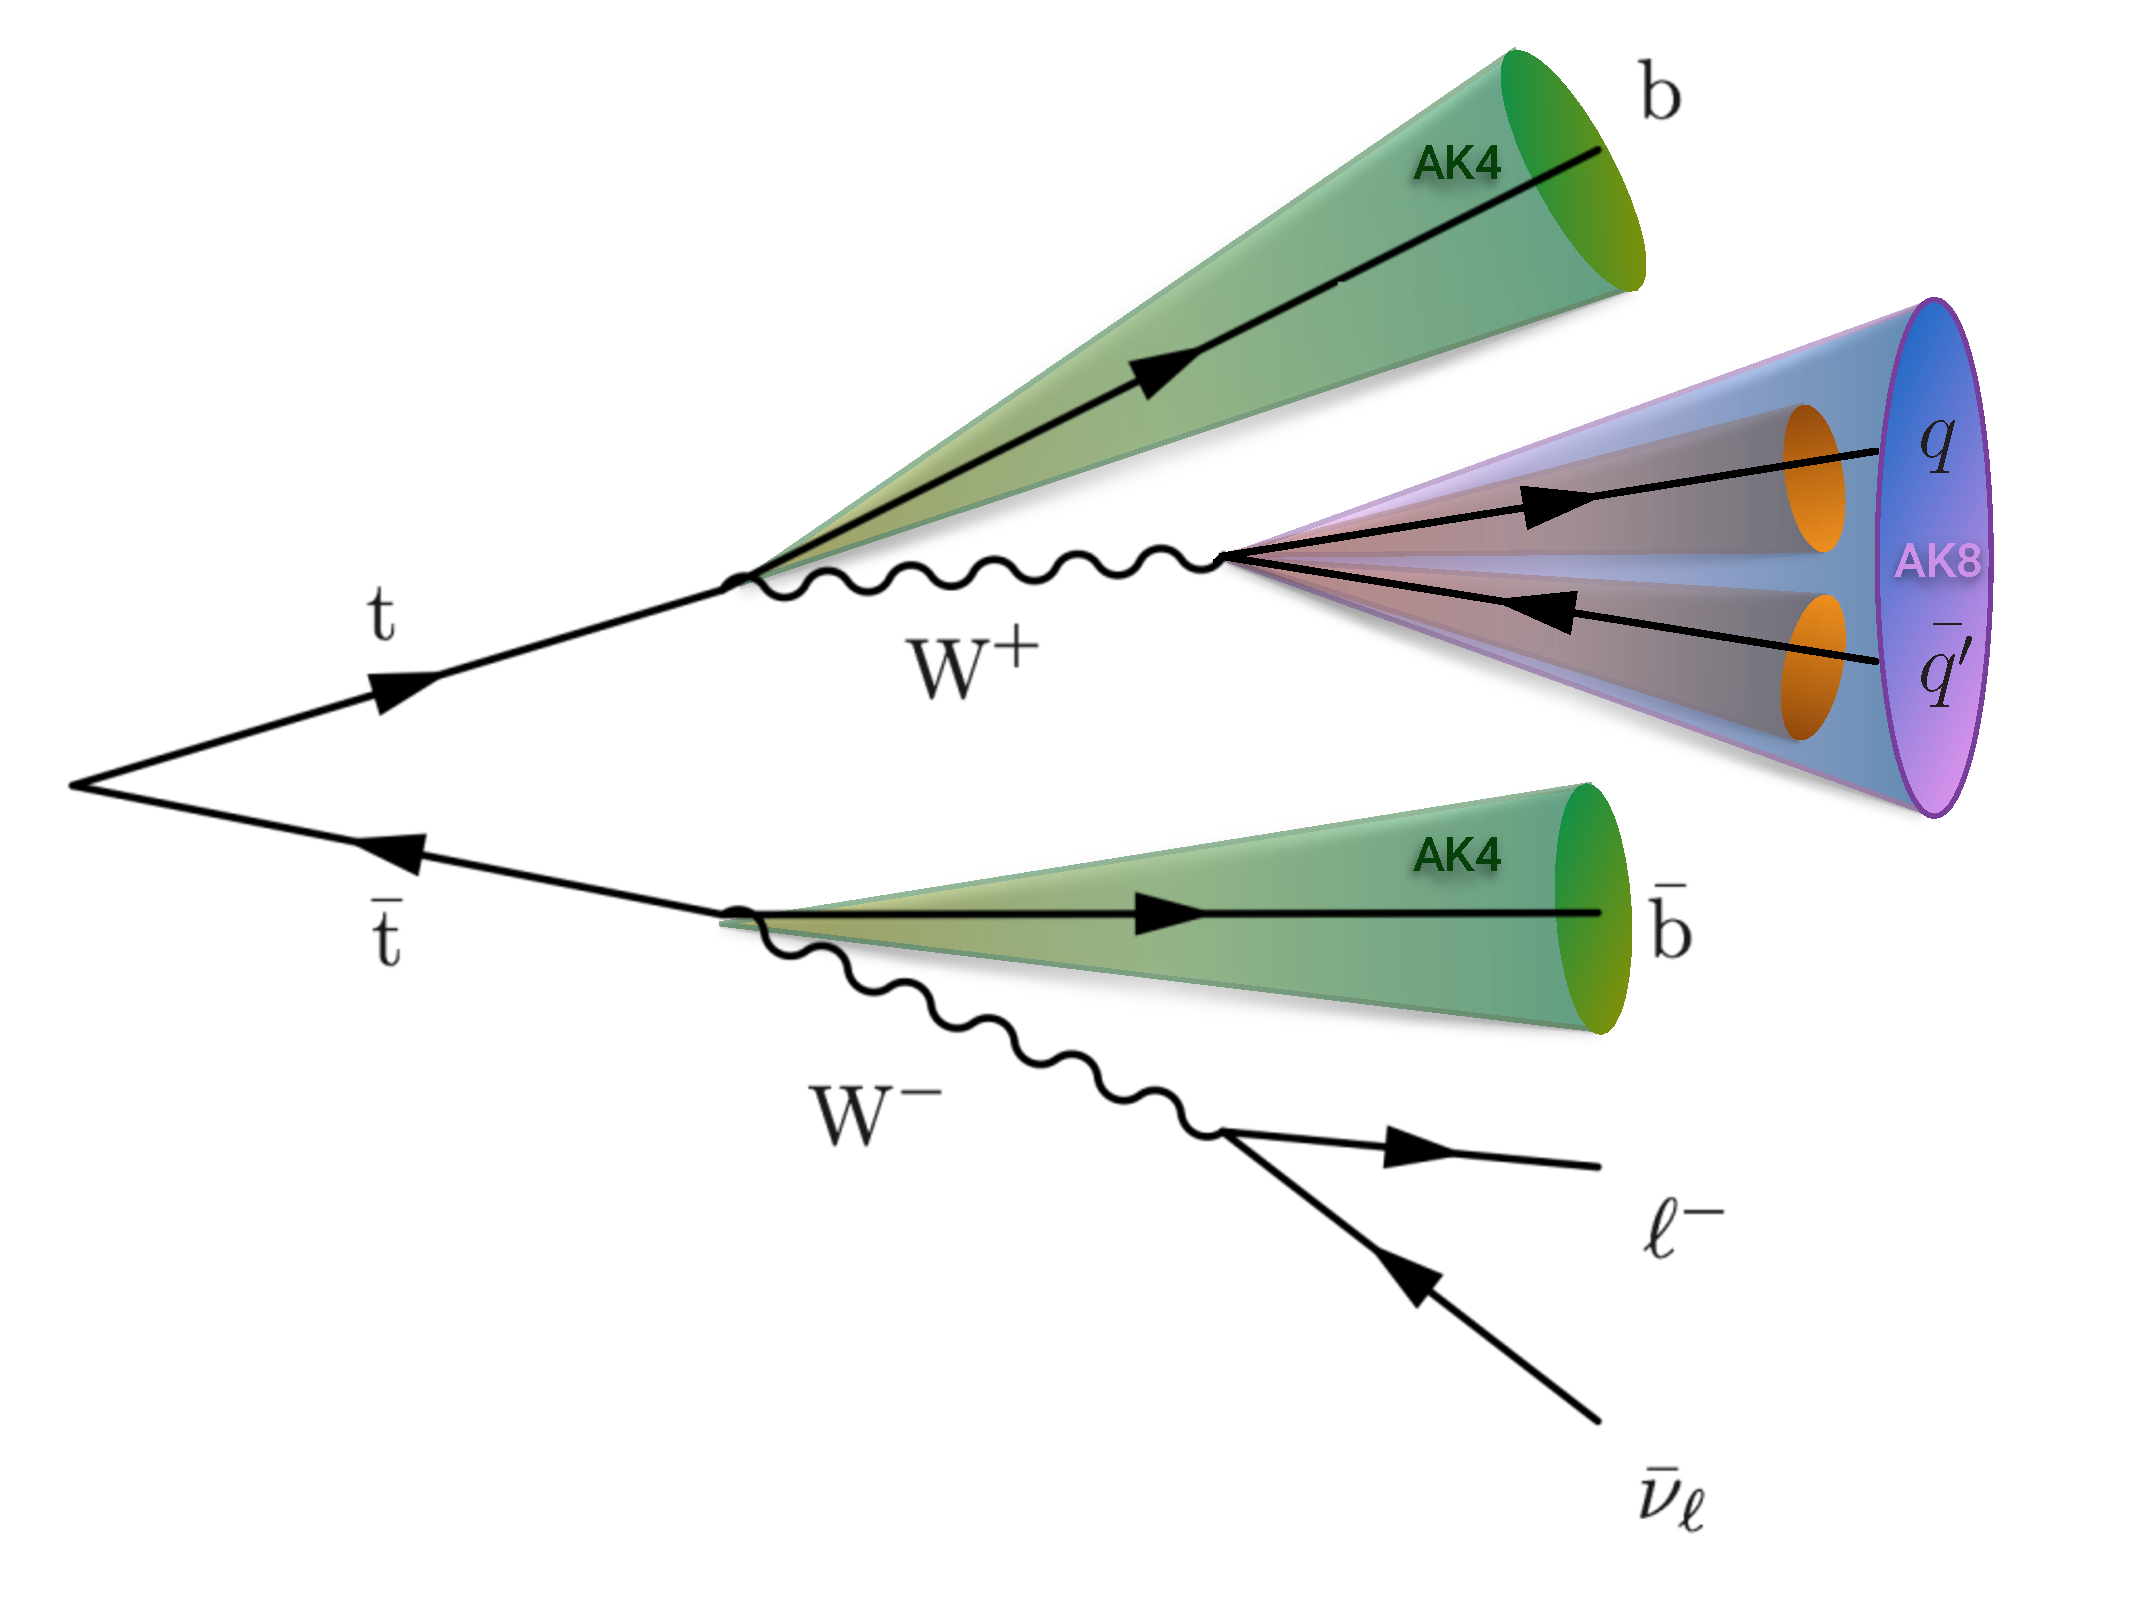
\includegraphics[width=0.49\textwidth]{figures/analysis/search2/misc/semileptt.pdf}
\caption{A top quark pair decaying into two b quarks and two \PW bosons, one of which decays leptonically and one on which decays hadronically}
\label{fig:search2:ttsemilep}
\end{figure}

\subsection{Event selection}
\label{sec:searchI:vtag:evsel}
The \PW can decay either to an electron or a muon, both final states ("channels") are used in the analysis. We select events through triggering and selections on the leptonic leg. First, we require a high-energy lepton at trigger level, with an online \PT above 45 \GeV for the muon and 135 \GeV for the electron. This requires an offline muon(electron) \PT threshold of 53(120) \GeV. The leptons are further required to pass the lepton requirements defined in Section~\ref{sec:objreco:muons} and Section~\ref{sec:objreco:electrons}, and events containing additional leptons (passing the same ID requirements, but looser cuts as defined in Table~\ref{tab:searchII:cutsummary}) are vetoed. Offline, we further require a high missing energy of 40(80) \GeV in the muon(electron) channel. To insure a high signal (boosted hadronic \PW) purity, the leptonic \PW four-vector is reconstructed such that we can put tight momentum requirements on the leptonic leg (ensuring that both tops, and therefore vector bosons, have a high momentum). The leptonic \PW is reconstructed in two steps: First, the unknown z component of the neutrino momentum must be solved for through a second order equation assuming the real \PW mass
\begin{equation*}
M_\mathrm{W}^2 = m_\ell^2   + 2(E_\ell E_\nu - p_{x_\ell}p_{x_\nu} - p_{y_\ell}p_{y_\nu} - p_{z_\ell}p_{z_\nu} ) = (80.4)^2.  
\end{equation*}
This results in a completely defined neutrino four-vector, which is then added to the lepton four-vector. The sum of the two defines the leptonic \PW and its momentum is required to be greater than 200 \GeV. \newline
Further, we require at least one AK R=0.4 jet to be b-tagged with the Combined Secondary Vertex (CSV) algorithm~\cite{1748-0221-8-04-P04013,1748-0221-13-05-P05011}. This algorithm exploits the relatively long lifetime of b quarks leading to the presence of a displaced vertex, in order to distinguish between jets originating from b quarks to those originating from light flavor quarks. More information on the CSV algorithm can be found in ~\cite{1748-0221-8-04-P04013,1748-0221-13-05-P05011}. The reason for requiring only one b-tagged jet is to ensure a high selection efficiency.\newline
Finally, we require at least one AK R=0.8 jet in the event with a momentum greater than 200 \GeV which will be the hadronic \PW candidate. It's pruned jet mass is required to be between 40 \GeV and 150 \GeV. After reconstructing and selecting all our objects, a set of angular selections are applied to ensure a diboson like topology. These are the following:
\begin{itemize}
\itemsep0em 
  \item $\Delta R(\l,W_{AK8}) > \pi/2$
  \item $\Delta \phi(W_{AK8},\ETmiss) > 2$
  \item $\Delta \phi(W_{AK8},W_{lep}) > 2$
\end{itemize}
With these requirements, we have a nearly pure sample of \ttbar events, with a small contamination from
single top, W+jets and \VV events.  A summary of the final selection criteria is presented in Table~\ref{tab:searchII:cutsummary}.The pruned jet mass and $\tau_{21}$ variables in data and in MC are shown in Figure~\ref{fig:searchI:ttbarcp}.
\begin{table}[h!]
\footnotesize
\centering
\begin{tabular}{lcc}
\hline 
\multicolumn{1}{c}{\textbf{Selection}} & \textbf{Value} & \textbf{Comments}\\
\hline
\multicolumn{1}{c}{\texttt{Tight} Lepton selection}\\
\cline{1-1}
Electron $\PT$ & $\PT > 120 \GeV$    & \\
Muon $\PT$ & $\PT > 53 \GeV$ & \\
Electron $\eta$ & $|\eta|_{\text{SC}} <2.5$ except [1.4442, 1.566] & Veto ECAL barrel-endcap transition.\\
Muon $\eta$  & $|\eta|<2.1$  & \\
\hline
\multicolumn{1}{c}{\texttt{Loose} Lepton selection}\\
\cline{1-1}
Electron $\PT$ & $\PT > 35 \GeV$    & \\
Muon $\PT$ & $\PT > 20 \GeV$ & \\
Electron $\eta$ & $|\eta|_{\text{SC}} <2.5$ except [1.4442, 1.566] & Veto ECAL barrel-endcap transition.\\
Muon $\eta$  & $|\eta|<2.4$  & \\
\hline
\multicolumn{1}{c}{AK8 jet selections}\\
\cline{1-1}
Jet $\PT$ &  $\PT >200~\GeV$ & For hadronic \\
Jet $\eta$  & $|\eta|<2.4$ & W reconstruction \\
\hline
\multicolumn{1}{c}{AK4 jet selections}\\
\cline{1-1}
Jet $\PT$ &  $\PT >30~\GeV$ & Used for b-tag \\
Jet $\eta$  & $|\eta|<2.4$ & jet selection\\
\hline
\multicolumn{1}{c}{\ETmiss selections}\\
\cline{1-1}
\ETmiss (electron channel) &  \ETmiss$>80~\GeV$ & \\
\ETmiss (muon channel) & \ETmiss$>40~\GeV$ & \\
\hline
\multicolumn{1}{c}{Boson selections}\\
\cline{1-1}
Pruned jet mass & $ 40 < m_{p} < 150 \GeV$ &  \\
Leptonic W $\PT$      &  $\PT > 200 \GeV$     & \\
Hadronic W $\PT$      &  $\PT > 200 \GeV$     & \\
\hline
\multicolumn{1}{c}{Veto}\\
\cline{1-1}
Number of \texttt{loose} electrons & 0    &  \\
Number of \texttt{loose} muons & 0    & \\
Number of b-tagged jets           & $>0$    & CSV medium working point \\
\hline
\multicolumn{1}{c}{Angular selections}\\
\cline{1-1}
$\Delta R(\l,W_{AK8})         $ & $> \pi/2$ & \\
$\Delta \phi(W_{AK8},\ETmiss) $ & $> 2$     & \\
$\Delta \phi(W_{AK8},W_{lep}) $ & $> 2$     & \\
\hline
\end{tabular}
\caption{Summary of the final semi-leptonic t$\bar{t}$ selections.}
\label{tab:searchII:cutsummary}
\end{table}

\begin{figure}[ht!]
\centering
\begin{tabular}{cc}
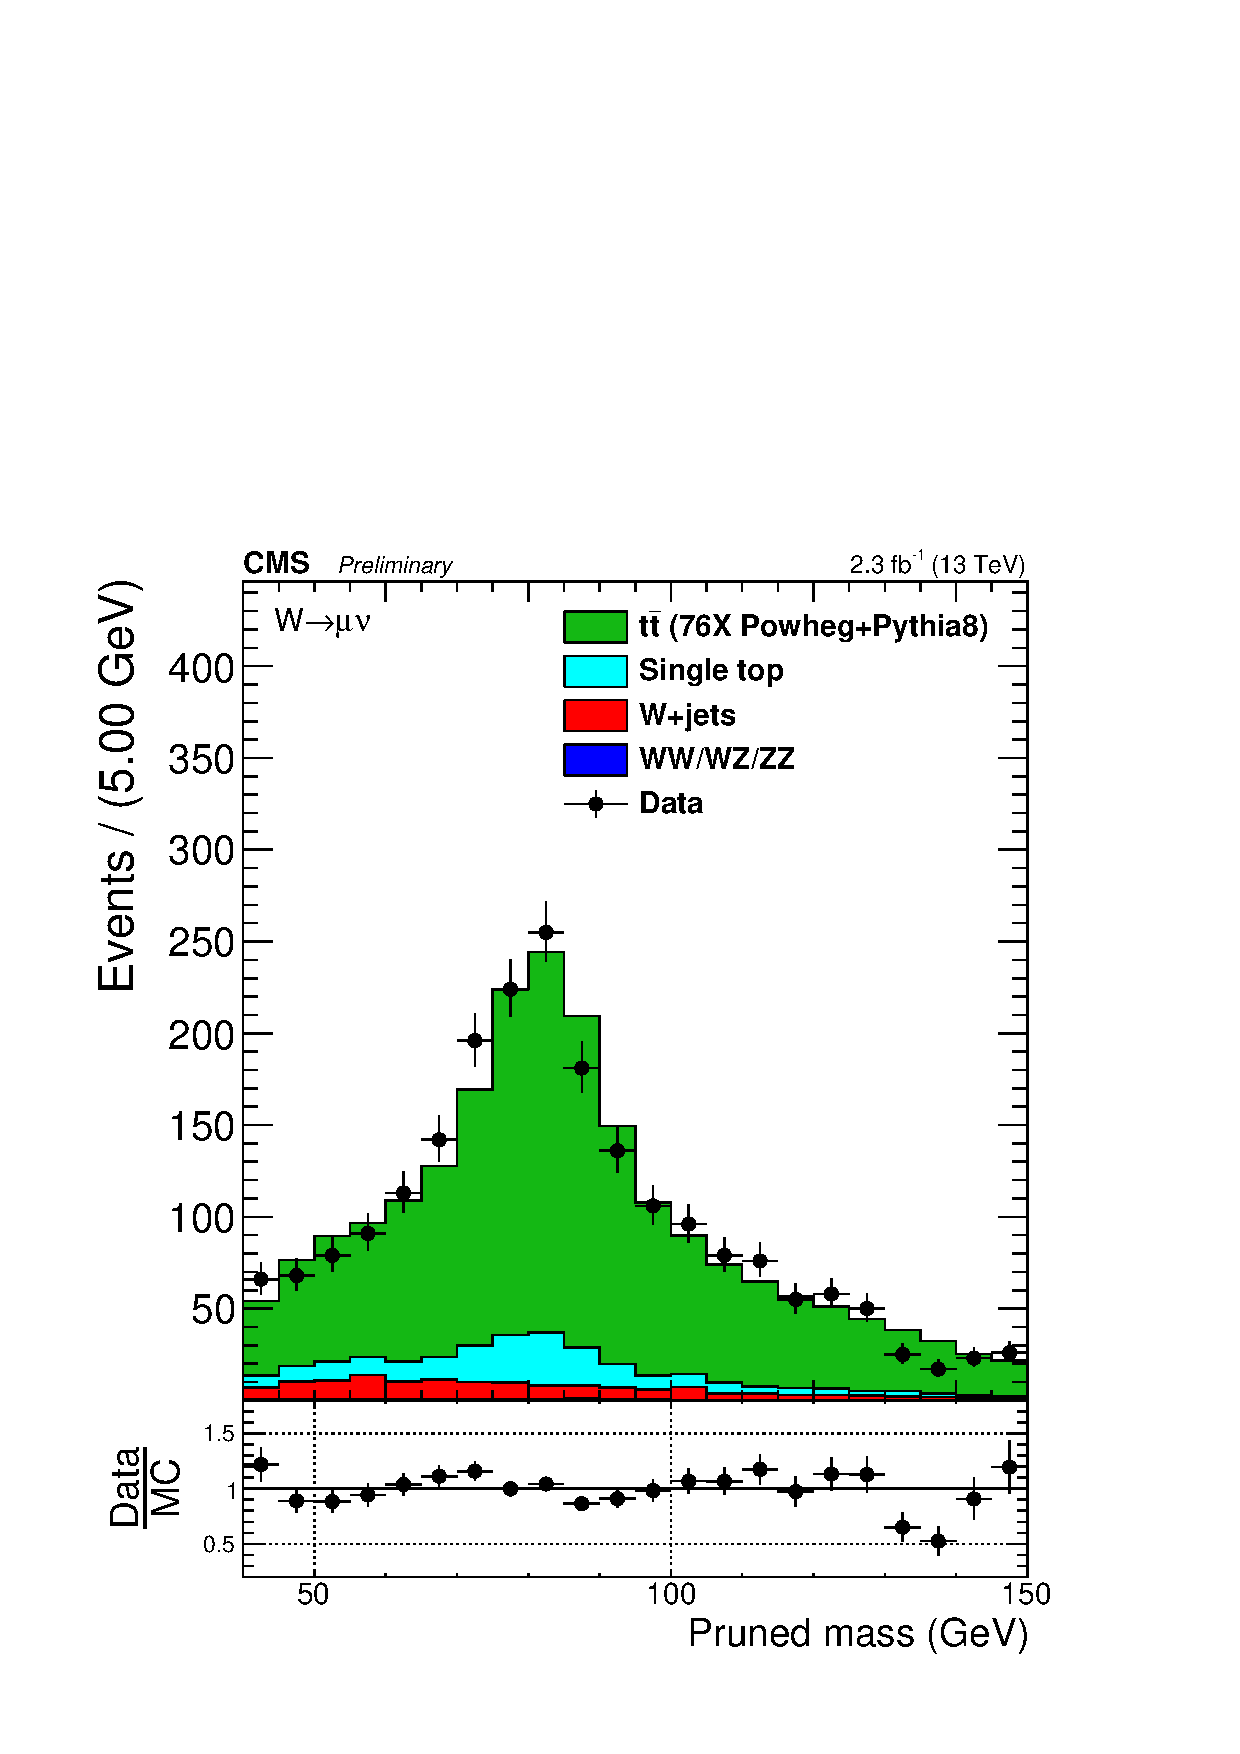
\includegraphics[width=0.4\textwidth]{figures/vtagging/AN-16-215/Whadr_pruned_mu.pdf}
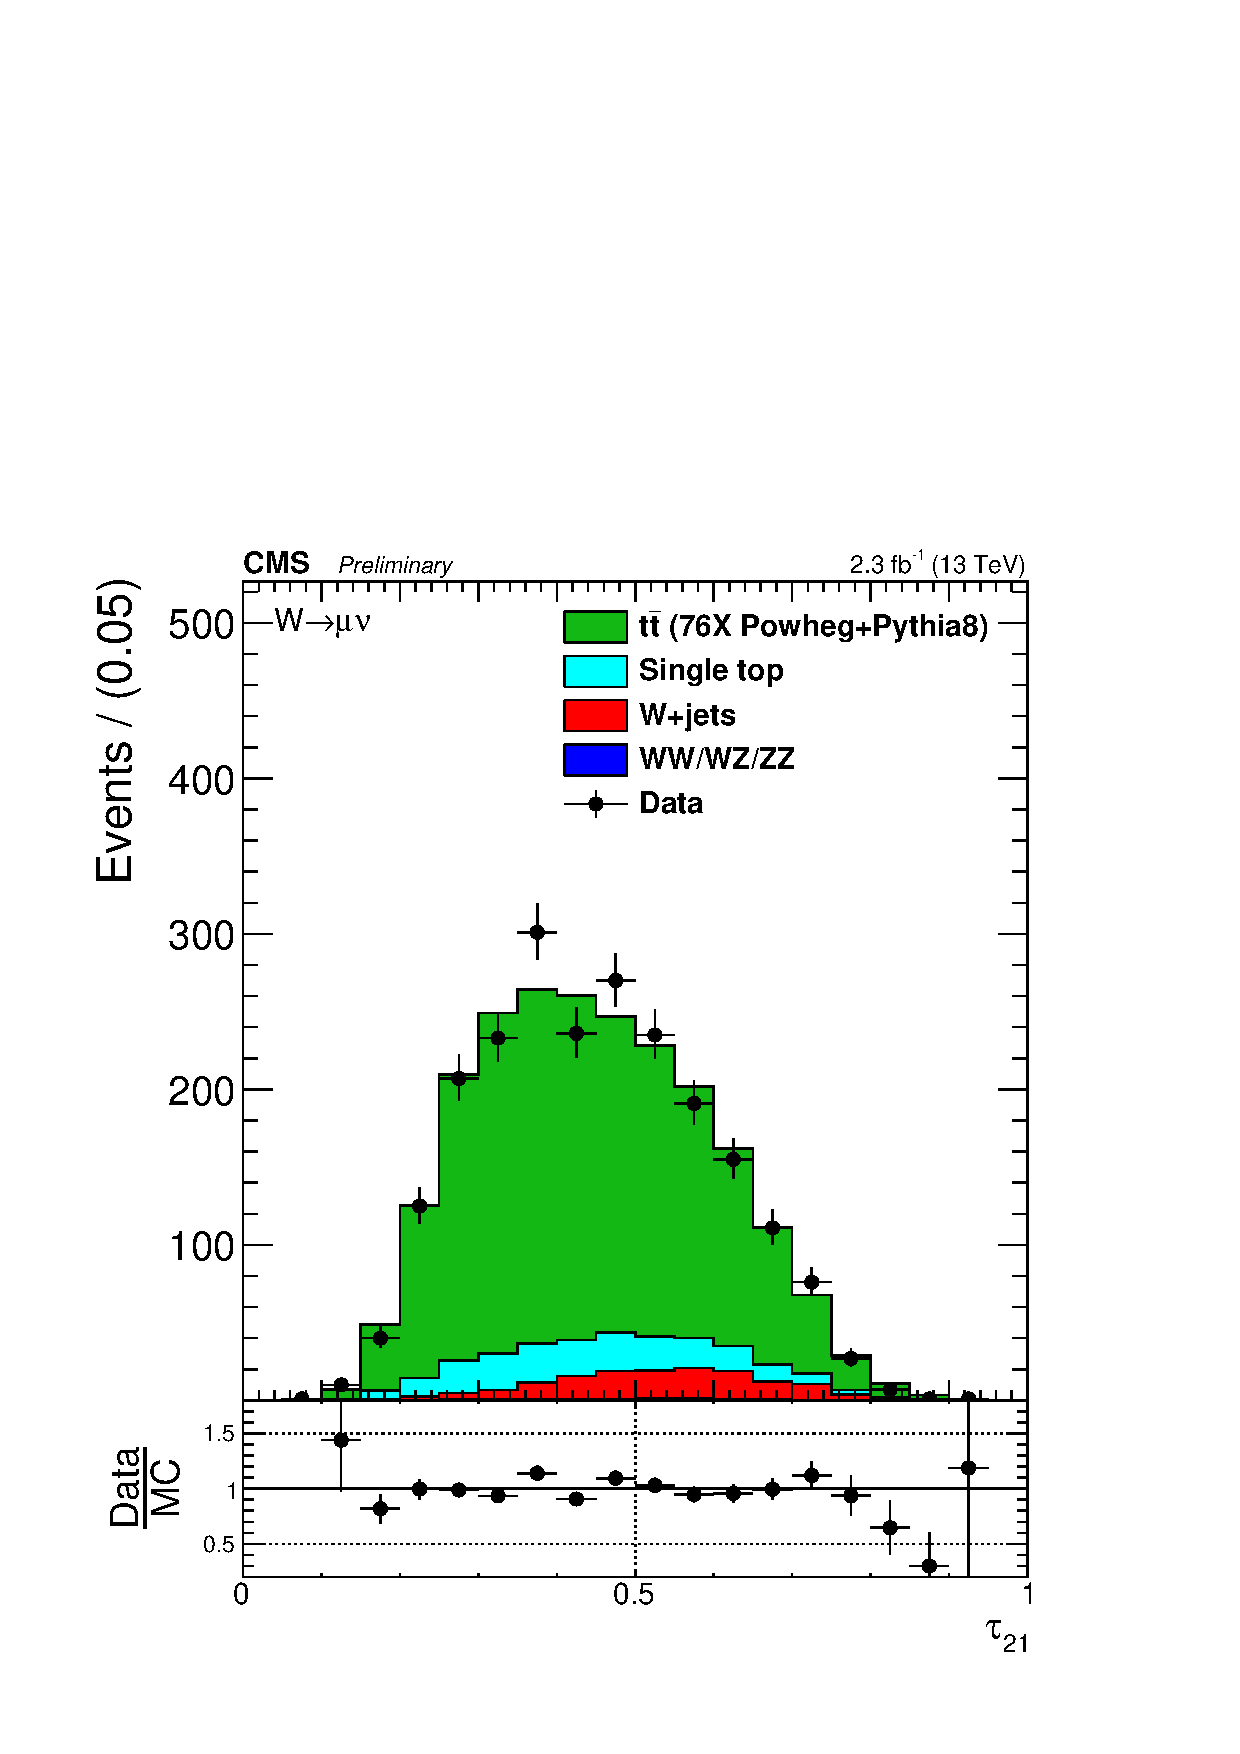
\includegraphics[width=0.4\textwidth]{figures/vtagging/AN-16-215/Whadr_tau21_mu.pdf}\\
% \includegraphics[width=0.5\textwidth]{figures/vtagging/AN-16-215/Whadr_puppi_softdrop_mu.pdf}
% \includegraphics[width=0.5\textwidth]{figures/vtagging/AN-16-215/Whadr_puppi_tau2tau1_mu.pdf}\\
\end{tabular}
\caption{Distribution of pruned jet mass (left) and n-subjettiness (right) in the \ttbar control sample.} 
\label{fig:searchI:ttbarcp}
\end{figure}

\subsection{Fitting procedure}
For this measurement, what we are interested in is to extract and compare the W-tagging efficiency of the combined jet mass and \nsubj selection in data and in MC. We are additionally interested in the difference in jet mass scale (mean of the \PW jet mass peak) and jet mass resolution (width of \PW jet mass peak), as this also affects the signal jet mass shape and therefore efficiency. In order to study these variables, we look at the pruned jet mass spectrum between 40 and 150 \GeV in two regions: 
\begin{itemize}
\itemsep0em 
  \item Pass region: $0 <  \nsubj \leq 0.45 \sim$ high purity
  \item Fail region: $0.45 < \nsubj \leq 0.75\sim$ low purity
\end{itemize}
Our goal is to understand what the real fraction of merged \PW jets is in the pass category and in the fail category, assuming that the sum of the two correspond to a 100\% selection efficiency (the amount of \PW jets falling outside of this region is negligible).
The strategy is the following: We first derive probability density functions (PDFs) which describe the distribution of fully merged \PW jets and non-\PW jets in \ttbar, both in the pass and in the fail region. The PDFs describing real \PW jets and non-\PW jets are added with a fraction which is left floating: the fit decides what the fraction of real \PW to non-\PW jets is in the pass and in the fail region. As simultaneous fit of pass and fail is then performed (using the two composite \PW+non-\PW PDFs), where the fraction of real \PW jets in both pass and fail is constrained such that, if the signal efficiency in pass is $\epsilon_S$, the signal efficiency in fail is ($1-\epsilon_S$). This is done by letting the normalization of the PDF describing real \PW jets in the pass category, be defined as the \textit{total} real \PW yield in pass and fail combined multiplied by some fraction, $\epsilon_S$. The normalization of the PDF describing real \PW jets in the fail category is then the total real \PW yield multiplied by ($1-\epsilon_S$).\newline
To understand which part of the \ttbar jet mass distribution contains ``real'' merged Ws and which are only pure combinatorial background, non-PWs, we start from \ttbar MC.
By matching the AK8 jet with quarks coming from the hadronic W at generator level, in a cone of $\Delta R < 0.8$, we can access the real merged \PW and non-merged \PW shapes.
The real \PW and non-\PW PDFs for jets that pass and fail the N-subjettiness selection $\nsubj < 0.45$, are found to be well described by the following functions:
\begin{align*} 
f_{\rm bkg}(m_{j}) &= F_{\textrm{ExpErf}} = e^{c_0m_{j}} \cdot \frac{1 + {\rm Erf}((m_{j}-a)/b)}{2}  &\sim\textrm{for non-\PW jets in both pass and fail }\\
f^{\rm sig}(m_{j}) &= F_{\rm Gaus}(m_{j}) + F_{\rm ExpErf}(m_{j})                                    &\sim\textrm{for real \PW jets in both pass and fail}
\end{align*}
Figure~\ref{fig:searchI:ttfitpruned} shows the fitted PUPPI softdrop mass spectrum for \ttbar real \PW (top) and non-\PW (bottom) distributions for jets that passed (left) and failed (right column) the N-subjettiness selection PUPPI $\tau_{21}~<$~0.4.
The corresponding plots for the jet pruned mass can be found in Figure~\ref{app:sf16}.

\begin{figure}[h!]
  \centering
      \includegraphics[width=0.3\textwidth]{figures/vtagging/AN-16-215/plots_76X/fits_TTMC/plots_em_HP0v45powheg_76X_MCfits/{_TTbar_realWExoDiBosonAnalysis.WWTree_TTbar_powheg_76X_GausErfExp_ttbar_with_pull}.pdf}
      \includegraphics[width=0.3\textwidth]{figures/vtagging/AN-16-215/plots_76X/fits_TTMC/plots_em_HP0v45powheg_76X_MCfits/{_TTbar_realW_failtau2tau1cutExoDiBosonAnalysis.WWTree_TTbar_powheg_76X_GausErfExp_ttbar_failtau2tau1cut_with_pull}.pdf}\\
      \includegraphics[width=0.3\textwidth]{figures/vtagging/AN-16-215/plots_76X/fits_TTMC/plots_em_HP0v45powheg_76X_MCfits/{_TTbar_fakeWExoDiBosonAnalysis.WWTree_TTbar_powheg_76X_ErfExp_ttbar_with_pull}.pdf}
      \includegraphics[width=0.3\textwidth]{figures/vtagging/AN-16-215/plots_76X/fits_TTMC/plots_em_HP0v45powheg_76X_MCfits/{_TTbar_fakeW_failtau2tau1cutExoDiBosonAnalysis.WWTree_TTbar_powheg_76X_ErfExp_ttbar_failtau2tau1cut_with_pull}.pdf}
    \caption{Fit to the real \PW (top) and non-\PW (bottom) pruned jet mass distribution for jets that pass (left) and fail (right) the cut on $\tau_{21}~<$~0.45.}
  \label{fig:searchI:ttfitpruned}
\end{figure}
These shapes constitute the fit functions used for the simultaneous fit. As can be seen from the fit to real \PW jets in the pass region, the distribution is not purely Gaussian and have a tail at higher groomed masses. This tail depends on the matching requirements used to define real merged \PW jets and is unphysical. We therefore assume that the distribution of real W-jets can be described by a Gaussian only, allowing the exponential error function  used to describe non W-jets to cover the contribution from the tails, hereby taking the number of real W-jets as the integral of the Gaussian shape only. This eliminates two additional fit functions, corresponding to six free parameters from the fit. 
In older estimations of the W-tagging scale factor based on the same procedure~\cite{CMS-PAS-B2G-16-021}), the functions used to describe the tail of the real W-jet distributions were also taken into account as contributing to the real W-jet tagging efficiency. These two calculations tests two extremes:
The new method assumes a Gaussian peak, absorbing the tails into the background function making the fit more robust, while the old method assumes a Gaussian peak with tails estimated from matched MC. The latter uses a more precise definition of real \PW jets, but a less robust fit. Both methods were investigated and we found that the absorption of tails into the background function resulted in a decrease in the relative uncertainty on the final scale factor of 50 $\%$ and an overall improvement on the fit quality, reducing the fit $\chi^2$ by 15 $\%$. The fit parameters of the functions used to describe non W-jets in both the pass and in the fail region, are further constrained using the values obtained from matched \ttbar MC. The W-tagging scale factors ($SF_{HP}$), for the high purity selection ($\nsubj<0.45$), are then extracted estimating the cut efficiency ($\epsilon_{HP}$) on both data and simulated samples fitting, simultaneously, pass and fail samples:
\begin{align*}
\footnotesize
    L_{\rm pass} &= \prod_{i}^{N_{\rm evt}^{pass}} \bigg[N_{\rm W}\cdot\epsilon_{HP}\cdot f_{\rm pass}^{\rm sig}(m_{j}) + N_{\rm 2}\cdot f_{\rm pass}^{\rm bkg}(m_{j})+ \sum_{j=\textrm{ST,VV,WJet}} N^{j}_{\rm pass}\cdot f_{\rm pass}^{j}\bigg]\\
    L_{\rm fail} &= \prod_{i}^{N_{\rm evt}^{fail}} \bigg[N_{\rm W}\cdot(1-\epsilon_{HP})\cdot f^{\rm sig}_{\rm fail}(m_{j}) + N_{\rm 3}\cdot f_{\rm fail}^{\rm bkg}(m_{j})+ \sum_{j=\textrm{ST,VV,WJet}} N^{j}_{\rm fail}\cdot f_{\rm fail}^{j}\bigg]
\end{align*}
where $N_{W}$ is the number of real W jets, $N_{2}$ and $N_{3}$ are the number of combinatorial background events passing and failing the \nsubj cut respectively. $N_{j}$ and $f_{j}$, with $j$ = ST, VV, WJet, are the normalizations and shapes of the minor backgrounds (single top, VV, W+jets) which are fixed from simulation. The fit functions used are
\begin{alignat*}{3}
    f_{\rm pass}^{\rm sTop} &= F_{\rm ErfExpGaus}(x) = &&\frac{1 + {\rm Erf}((x-a)/b)}{2} \cdot e^{-(x-x_{0})^{2}/2\sigma^{2}}\\
    f_{\rm fail}^{\rm sTop} &= F_{\rm ExpGaus}(x)    = &&e^{ax} \cdot e^{-(x-b)^{2}/2s^{2}}\\
    f_{\rm pass}^{\rm VV}   &= F_{\rm ExpGaus}(x)    = &&e^{ax} \cdot e^{-(x-b)^{2}/2s^{2}}\\
    f_{\rm fail}^{\rm VV}   &= F_{\rm ExpGaus}(x)    = &&e^{ax} \cdot e^{-(x-b)^{2}/2s^{2}}\\
    f_{\rm pass}^{\rm wjet} &= F_{\rm ErfExp}(x)     = &&e^{c_0x} \cdot \frac{1 + {\rm Erf}((x-a)/b)}{2}\\
    f_{\rm fail}^{\rm wjet} &= F_{\rm ErfExp}(x)     = &&e^{c_0x} \cdot \frac{1 + {\rm Erf}((x-a)/b)}{2}
\end{alignat*}
with the corresponding distributions shown in Figure~\ref{fig:searchII:minorbkr}.
\begin{figure}[h!]
   \centering
    \includegraphics[width=0.30\textwidth]{figures/vtagging/AN-16-215/plots_76X/plots_0v45/plots_em_HP0v45powheg_76X_MCfits/{_STopExoDiBosonAnalysis.WWTree_STop_76X_ErfExpGaus_sp}.pdf}
    \includegraphics[width=0.30\textwidth]{figures/vtagging/AN-16-215/plots_76X/plots_0v45/plots_em_HP0v45powheg_76X_MCfits/{_WJets0ExoDiBosonAnalysis.WWTree_WJets_76X_ErfExp}.pdf}
    \includegraphics[width=0.30\textwidth]{figures/vtagging/AN-16-215/plots_76X/plots_0v45/plots_em_HP0v45powheg_76X_MCfits/{_VVExoDiBosonAnalysis.WWTree_VV_76X_ExpGaus}.pdf}\\
    \includegraphics[width=0.30\textwidth]{figures/vtagging/AN-16-215/plots_76X/plots_0v45/plots_em_HP0v45powheg_76X_MCfits/{_STop_failtau2tau1cutExoDiBosonAnalysis.WWTree_STop_76X_ExpGaus}.pdf}
    \includegraphics[width=0.30\textwidth]{figures/vtagging/AN-16-215/plots_76X/plots_0v45/plots_em_HP0v45powheg_76X_MCfits/{_WJets0_failtau2tau1cutExoDiBosonAnalysis.WWTree_WJets_76X_ErfExp}.pdf}
    \includegraphics[width=0.30\textwidth]{figures/vtagging/AN-16-215/plots_76X/plots_0v45/plots_em_HP0v45powheg_76X_MCfits/{_VV_failtau2tau1cutExoDiBosonAnalysis.WWTree_VV_76X_ExpGaus}.pdf}
  \caption{Fits to the pruned jet mass spectrum for the non-dominant backgrounds (Single top, W+jets and VV respectively) in the pass (top) and fail (bottom) regions.}
  \label{fig:searchII:minorbkr}
\end{figure} 
The floating parameters of the fit (besides the PDF shape parameters themselves) are the rates $N_{W}$, $N_{2}$ and $N_{3}$, and the mean and sigma of the W-mass distribution defined in
$f^{\rm sig}_{\rm pass}(m_{j})$ and $f^{\rm sig}_{\rm fail}(m_{j})$. The ratio between data and simulation efficiencies are then taken as the W-tagging scale factor:
\begin{equation}
  \label{SF}
  SF_{HP}= \frac{\epsilon_{HP}(\textrm{data})}{\epsilon_{HP}(\textrm{sim})}
\end{equation}
Considering that, both for data and simulation, $\epsilon_{HP}+\epsilon_{LP}+\epsilon_{fail} = 1$, the scale factor for low purity category can be defined as:
\begin{equation*}
  SF_{LP} = \frac{1-\epsilon_{HP}(\textrm{data})-\epsilon_{fail}(\textrm{data})}{1-\epsilon_{HP}(\textrm{sim})-\epsilon_{fail}(\textrm{sim})}
\end{equation*}
where $\epsilon_{fail}$ is the ratio between the number of events with $\tau_2/\tau_1 > 0.75$ and the total number of events. As mentioned previously, the number of real \PW jets with $\tau_2/\tau_1 > 0.75$  is negligible and the definition of the low purity scale factor simplifies to
\begin{equation}
  SF_{LP} = \frac{1-\epsilon_{HP}(\textrm{data})}{1-\epsilon_{HP}(\textrm{sim})}
\end{equation}

\subsection{Systematic uncertainties}
\label{sec:searchI:wtagsystematic}
As systematic uncertainties, we consider effects due to differences in \ttbar simulation as well as effects due to choice of fit method. The former is evaluated by comparing the extracted scale factor when using \ttbar MC samples produced with different matrix element (ME) and shower generators: \POWHEG (NLO) interfaced with \PYTHIA{8} , \MADGRAPH (LO) QCD interfaced with \HERWIG{++} and \POWHEG interfaced with \HERWIG{++}.
The uncertainty due to different ME generators (\POWHEG versus \MADGRAPH) correspond to 3(13)\% and are listed in Table~\ref{tab:searchI:WtagSFs} as the first quoted systematic uncertainty. The uncertainty due to parton showering (\PYTHIA{8} versus \HERWIG{++}) is 8.6\%, but are not relevant for analyses where no \HERWIG{++} based simulation is used, as is the case for the search presented in this chapter. 
For the systematic uncertainty accounting for effects due to choice of fit method, we compare the estimated extracted efficiency in \ttbar MC using the two different fit models described above: The new model, where the signal is modeled by a Gaussian peak and the tails of the distribution are absorbed in the background fit model, and the old model, including the tails when calculating the fraction of real \PW jets. Figure~\ref{fig:searchII:gausvstails} shows the fits obtained in the pass and fail regions using the two different models. With the new model only the Gaussian component of the fit contributes to the W-tagging efficiency while, with the old model, a Chebyshev component is additionally contributing to the total W-tagging efficiency.
\begin{figure}[ht!]
  \centering
    \includegraphics[width=0.33\textwidth]{figures/vtagging/AN-16-215/2Gauss.pdf}
    \includegraphics[width=0.33\textwidth]{figures/vtagging/AN-16-215/GausErfExpPass.pdf}\\
    \includegraphics[width=0.33\textwidth]{figures/vtagging/AN-16-215/GausChebysgev.pdf}
    \includegraphics[width=0.33\textwidth]{figures/vtagging/AN-16-215/GausErfExpFail.pdf}
  \caption{Fits obtained in the pass (top) and fail (bottom) regions using two different models: An alternative model with tails (top and bottom, left) where the tail component is contributing to the total W-tagging efficiency. When using the default model (top and bottom, right), only the Gaussian component of the fit contributes to the W-tagging efficiency.}
  \label{fig:searchII:gausvstails}
\end{figure} 
The estimated efficiencies obtained using both methods, after being corrected for the fraction of \PW jets in the tails, agree within 0.3(0.8)\% and are listed as systematic uncertainty in Table~\ref{tab:searchI:WtagSFs}.\newline
One additional uncertainty is added. As the W-tagging scale factor is evaluated in a \ttbar sample, the transverse momentum range is rather limited. When the \PW \PT reaches $\sim 400 \GeV$, the AK8 jet becomes a fully merged top jet with a mass of 170 \GeV and a scale factor measurement becomes impossible. However, the jets used in the analyses presented in this thesis have very high transverse momenta, up to 2-3 \TeV, and we therefore need an estimate of how the uncertainty on the W-tagging scalefactor changes as a function of \PT. This is estimated by comparing the difference in tagging between $\BulkG \rightarrow \PW \PW$ signal MC showered by \PYTHIA{}8 and \HERWIG{++} as a function of \PT, relative to the difference in tagging efficiency between the two at a $\PT \sim 200$~\GeV. This measurement was performed by a separate analysis team, and found to be $5.90\% \times \ln(\pt/200\GeV)$.

% \begin{figure}[h!]
%   \centering
%     \includegraphics[width=0.50\textwidth]{figures/vtagging/AN-16-215/wtag-ptdependence-tau21tight.pdf}
%   \caption{Uncertainty on the \pt dependence of the scale factor as a function of \pt, approximated with a logarithmic function.}
%   \label{fig:ptdependence}
% \end{figure}

Systematic uncertainties from other sources (lepton identification, b tagging etc.) are less than 0.5\% and therefore negligible.

\subsection{Fit results}
The simultaneous fit as described above is then performed both for data and for simulation, where we take the ratio of data and MC efficiencies as efficiency scale factors.
The corresponding fits are shown in Figure~\ref{fig:searchII:simfit}, with the corresponding extracted efficiencies and scale factors summarized in Table~\ref{tab:searchI:WtagSFs}.

\begin{table}[h!]
   \centering
   \footnotesize
   \begin{tabular}{| l | c | c | c | c |}
   \hline
   Category & Working point & Eff. data & Eff. simulation & Scale factor\\
   \hline
   HP&$\tau_2 / \tau_1 < 0.45$& $0.775 \pm 0.041 $& $0.822 \pm 0.033$ &$0.94 \pm 0.05~\rm{(stat)} \pm 0.03~\rm{(sys)} \pm 0.003~\rm{(sys)}$\\
   LP&$0.45 < \tau_2 / \tau_1 < 0.75$& $0.225 \pm 0.041 $& $0.178 \pm 0.033$ &$1.27 \pm 0.25~\rm{(stat)} \pm 0.13~\rm{(sys)} \pm 0.008~\rm{(sys)}$\\
   \hline
   \end{tabular}
   \caption{Efficiencies in data and in MC together with the corresponding W-tagging scale factors for the high purity and low purity categories. }
   \label{tab:searchI:WtagSFs}
\end{table}


\begin{figure}[h!]
\centering
\includegraphics[width=0.44\textwidth]{figures/vtagging/AN-16-215/_HP0v45powheg_76X_em_pTbin_200_5000.pdf}
\includegraphics[width=0.44\textwidth]{figures/vtagging/AN-16-215/_HP0v45powheg_76X_em_fail_pTbin_200_5000.pdf} \\
\caption{Pruned jet mass distribution that pass (left) and fail (right) the $\tau_2 / \tau_1 < 0.45$ selection. Results of both the fit to data (blue) and simulation(red) are shown. The background components of the fit are shown as short-dashed lines.}
\label{fig:searchII:simfit}
\end{figure}

We additionally extract the jet mass scale and jet mass resolution, used to scale and smear the jet mass signal shape in the limit setting procedure. These values are taken from the mean $\langle m \rangle$ and width $\sigma$ of the Gaussian
component of the simultaneous fit in the pass region and are summarized in Table~\ref{tab:searchI:params}. Both the jet mass scale as well as the jet mass resolution is larger in simulation than in data with a relative difference of 2 and 10\%, respectively.
Howver, the jet mass resolution scale factor has a large uncertainty attached to it and is statistically insignificant (in agreement with unity within uncertainty).

\begin{table}[!htb]
 \begin{center}

 \begin{tabular}{|l|c|c|c}
  Parameter & Data & Simulation & Data/Simulation \\
  \hline
  Pruning $\langle m \rangle$ &$80.9 \pm 0.6~{\rm \GeV}$   & $82.5 \pm 0.1~{\rm \GeV}$  & $0.980 \pm 0.007$ \\
  Pruning $\sigma$            & \ $6.7 \pm 0.7~{\rm \GeV}$ & \ $7.5 \pm 0.3~{\rm \GeV}$ & $0.89 \pm 0.10$ \\
  \hline
  % PUPPI softdrop $\langle m \rangle$ &$86.8 \pm 0.8~{\rm \GeV}$ & $87.9 \pm 0.2~{\rm \GeV}$ & $0.988 \pm 0.010$ \\
%   PUPPI softdrop $\sigma$ & \ $9.2 \pm 1.0~{\rm \GeV}$ & \ $8.7 \pm 0.4~{\rm \GeV}$ & $1.07 \pm 0.09$ \\
  % PUPPI softdrop $\langle m \rangle$ &$80.3 \pm 0.8~{\rm \GeV}$ & $81.9 \pm 0.01~{\rm \GeV}$ & $0.98 \pm 0.01$ \\%New mass corrections
  % PUPPI softdrop $\sigma$ & \ $9.0 \pm 0.9~{\rm \GeV}$ & \ $8.5 \pm 0.4~{\rm \GeV}$ & $1.07 \pm 0.12$ \\%New mass corrections
 \end{tabular}
 \caption{Jet mass scale and resolution in data and in simulation together with the relevant data-simulation scale factors.}
 \label{tab:searchI:params}
 \end{center}
\end{table}

\subsection{Impact on search variables}
\label{sec:searchI:wtagimpact}

The obtained W-tagging scale factors are used as a scale of the signal yield. As we require two W-tagged jets, either HPHP or HPLP, the actual scale factors for the high-purity signal yield is $\textrm{SF}_{HP}\times\textrm{SF}_{HP}$ and for the low-purity category $\textrm{SF}_{HP}\times\textrm{SF}_{LP}$. The signal yields are then
\begin{align*}
N_{S}^{HP} &= N_{\textrm{HP tot. yield}} \times \textrm{SF}_{HP} \times \textrm{SF}_{HP}\\
N_{S}^{LP} &= N_{\textrm{LP tot. yield}} \times \textrm{SF}_{HP} \times \textrm{SF}_{LP}\\
\end{align*}
The uncertainties on the scale factors are considered as anti-correlated between the HP and the LP categories.
The jet mass scale and resolution are used to scale and smear the signal Monte Carlo. An uncertainty on the signal yield based on the uncertainty on jet mass scale and resolution is also considered by scaling and smearing the jet mass up and down within the quoted uncertainties and then recomputing the signal efficiency. The results are listed in Table~\ref{tab:searchI:sys}.
% With a HP relative uncertainty of 6\% and LP relative uncertainty of 22\%, this becomes
% \begin{align*}
% \sigma_{rel}^{HPHP} &= 1.06 \times 1.06 = 1.12\\
% \sigma_{rel}^{HPLP} &= 1.28 \times 1.06 = 1.36\\
% \end{align*}
  
\section{Systematic uncertainties}
\label{sec:searchI:sys}

The uncertainty on the background parametrization is statistical only and is taken as the covariance matrix of the dijet fit function. As demonstrated in the F-test, we study different background parameterizations and we have found these to be within the fit uncertainty of the nominal fit. The remaining uncertainties concern the signal shape and yield and are listen in Table~\ref{tab:searchI:sys}. Jet reconstruction uncertainties affect both the signal yield and she signal shape. These are evaluated by rescaling the jet four-momenta according to uncertainties on the jet energy scale and resolution and recomputing the signal efficiency. The difference in efficiency with and without smearing/scaling is taken as systematic uncertainties, as described above.
The jet mass/energy scale and resolution also affect the signal shape, and are added as uncertainties in the peak position and width of the Gaussian component of the signal PDFs.

\begin{table}[h!]
  \centering
  \begin{tabular}{lccc}
    \hline
    Source                           & Relevant quantity    & HP uncertainty (\%)  & LP uncertainty (\%)\\
    \hline
    Jet energy scale                 & Resonance shape      & 2                    & 2 \\
    Jet energy resolution            & Resonance shape      & 10                   & 10 \\
    \hline
    Jet energy and \mJ{} scale       & Signal yield         & \multicolumn{2}{c}{0.1--4}\\ 
    Jet energy and \mJ{} resolution  & Signal yield         & \multicolumn{2}{c}{0.1--1.4}\\
    Pileup                           & Signal yield         & \multicolumn{2}{c}{2}\\
    Integrated luminosity            & Signal yield         & \multicolumn{2}{c}{2}\\
    PDFs (\PWpr)                     & Signal yield		      & \multicolumn{2}{c}{4--19}\\
    PDFs (\PZpr)                     & Signal yield		      & \multicolumn{2}{c}{4--13}\\
    PDFs (\BulkG)                    & Signal yield		      & \multicolumn{2}{c}{9--77}\\
    Scales (\PWpr)                   & Signal yield		      & \multicolumn{2}{c}{1--14}\\
    Scales (\PZpr)                   & Signal yield		      & \multicolumn{2}{c}{1--13}\\
    Scales (\BulkG)                  & Signal yield		      & \multicolumn{2}{c}{8--22}\\
    \hline
    Jet energy and \mJ{} scale       & Migration            & \multicolumn{2}{c}{1--50}\\
    V tagging \nsubj{}               & Migration            & 14                    & 21\\
    V tagging \pt-dependence         & Migration            & 7--14                & 5--11\\
    \hline
  \end{tabular}
  \caption{Summary of  systematic uncertainties and the quantities they affect. Migration uncertainties result in events switching between the purity/mass categories and changes the efficiency in each category, but do not affect the total signal efficiency.}
  \label{tab:searchI:sys}
\end{table}


\clearpage

\section{Results}
\label{sec:searchI:results}
The background fits for each analysis category in the data signal region are shown in Figure \ref{fig:search1:bkgfitMassCat}. Here a background only fit is performed while, as described above, a simultaneous fit is used for the limit setting procedure. The filled area correspond to the 1 sigma error band of the background fit, obtained using linear error propagation.

\begin{figure}[h!]
\centering
\includegraphics[width=0.44\textwidth]{figures/analysis/search1/AN-15-211/fits/MLfits/BkgFit_DijetMassHighPuriWW.pdf}
\includegraphics[width=0.44\textwidth]{figures/analysis/search1/AN-15-211/fits/MLfits/BkgFit_DijetMassLowPuriWW.pdf}\\
\includegraphics[width=0.44\textwidth]{figures/analysis/search1/AN-15-211/fits/MLfits/BkgFit_DijetMassHighPuriWZ.pdf}
\includegraphics[width=0.44\textwidth]{figures/analysis/search1/AN-15-211/fits/MLfits/BkgFit_DijetMassLowPuriWZ.pdf}\\
\includegraphics[width=0.44\textwidth]{figures/analysis/search1/AN-15-211/fits/MLfits/BkgFit_DijetMassHighPuriZZ.pdf}
\includegraphics[width=0.44\textwidth]{figures/analysis/search1/AN-15-211/fits/MLfits/BkgFit_DijetMassLowPuriZZ.pdf}\\
\caption{Fit to data in the signal region using the background fit only for the different mass and purity categories. The filled red area correspond to the 1 sigma statistical error of the fit.}
\label{fig:search1:bkgfitMassCat}
\end{figure}

We proceed by setting limits on the cross section of the process $\text{X} \to \VV$, using the asymptotic $\textrm{CL}_\textrm{S}$ method as described in Section~\ref{sec:theory:statmet}. The binned likelihood is defined as
\begin{equation}
L = \prod_i\frac{\mu^{n_i}_ie^{-\mu_i}}{n_i!}
\end{equation}
with
\begin{equation}
\mu_i=\sigma \cdot N_i(S)+N_i(B)
\end{equation}
Here $\sigma$ is the signal strength scaling the expected number of signal events in the $i$-th dijet invariant mass bin $N_i(S)$, $N_i(B)$ is the expected number of background events in dijet invariant mass bin $i$ and $n_i$ is the observed number of events in the $ith$ dijet invariant mass bin. The background per bin $N_i(B)$ is estimated from the background component of the best signal+background fit to the data points with the signal cross section set to zero. The number of signal events in the $i$-th dijet invariant mass bin, $N_i(S)$, is then estimated from the signal templates, where only a dijet invariant mass in a 20\% window around the resonance mass is considered, containing most of the signal contribution while making sure to keep a good description of the core.

\section{Limits: All-hadronic analysis}
\label{sec:searchI:results4q}
As mentioned in Section~\ref{sec:searchI:samples}, we set limits on three different signal scenarios: $\BulkG \rightarrow \WW$, $\BulkG \rightarrow \ZZ$ and $\PWpr \rightarrow WZ$, with a $\ktilde = 0.5$ for the \BulkG. Figure \ref{fig:searchI:Limits_CombNew} shows the asymptotic limits at 95 \% confidence level on signal cross section as a function of the resonance mass obtained with 2.7 \fbinv of 13 \TeV CMS data after combining all mass and purity categories (top). The corresponding p-values are shown in the bottom panel.

\begin{figure}[h!]
\centering
\includegraphics[width=0.32\textwidth]{figures/analysis/search1/AN-15-211/limits/brazilianFlag_BulkWW_new_combined_13TeV.pdf}
\includegraphics[width=0.32\textwidth]{figures/analysis/search1/AN-15-211/limits/brazilianFlag_WZ_new_combined_13TeV.pdf}
\includegraphics[width=0.32\textwidth]{figures/analysis/search1/AN-15-211/limits/brazilianFlag_BulkZZ_new_combined_13TeV.pdf}\\
\includegraphics[width=0.32\textwidth]{figures/analysis/search1/AN-15-211/pvalues/pvalue_BulkWWin_combined_new.pdf}
\includegraphics[width=0.32\textwidth]{figures/analysis/search1/AN-15-211/pvalues/pvalue_WZin_combined_new.pdf}
\includegraphics[width=0.32\textwidth]{figures/analysis/search1/AN-15-211/pvalues/pvalue_BulkZZin_combined_new.pdf}\\
\caption{Expected and observed limits with corresponding p-values obtained using 2.6 $\textrm{fb}^{-1}$ of CMS data after combining all mass and purity categories. Here for a Bulk $G\rightarrow WW$ (left), $W'\rightarrow WZ$ (middle) and $G\rightarrow ZZ$ (right) signal.}
\label{fig:searchI:Limits_CombNew}
\end{figure}


The statistics are too low to exclude the excess around 2 \TeV observed in the corresponding Run 1 analysis and in addition an under-fluctuation in data is present in this region. The largest excess is observed for a $\BulkG \rightarrow \ZZ$ hypothesis at a resonance mass of 2.8-3 TeV, around 2.3 $\sigma$.
This is driven by the ZZ high-purity category, the category with the lowest statistics, where one event at 3 TeV yields a local significance of 2.8 $\sigma$. A 3-parameter fit is the default background fit function for this category, however, a 2-parameter fit could also be used to describe these data. In Figure \ref{fig:searchI:Limits_ZZHP} we compare the limits and p-values obtained using a 2-parameter and a 3-parameter fit to describe the background in this category. The significance at 3 TeV is reduced from 2.8 to 1.5 $\sigma$ with a 2-parameter fit, reflecting the fact that the fit is poorly constrained in the high mass tail due to low statistics. The fit to data using both a 2 and 3-parameter fit in the ZZHP category is shown in Figure~\ref{fig:app:ZZHP2vs3p} and we in addition see that the 2-parameter fit lies within the fit uncertainties of the nominal fit.\newline
\newline

\begin{figure}[h!]
\centering
\includegraphics[width=0.49\textwidth]{figures/analysis/search1/AN-15-211/limits/brazilianFlag_BulkZZ_ZZHP_13TeV.pdf}
\includegraphics[width=0.49\textwidth]{figures/analysis/search1/AN-15-211/limits/brazilianFlag_BulkZZ_ZZHP_2parFit__13TeV.pdf}\\
\includegraphics[width=0.49\textwidth]{figures/analysis/search1/AN-15-211/pvalues/pvalue_BulkZZinZZ_high_purity.pdf}
\includegraphics[width=0.49\textwidth]{figures/analysis/search1/AN-15-211/pvalues/pvalue_BulkZZinZZ_high_purity_2par.pdf}
\caption{Expected/observed limits and corresponding p-values obtained in the ZZHP category using a 3 (left) and two (right) parameter fit to describe the background. The significance at 3 TeV is reduced from 2.8 to 1.5 $\sigma$.}
\label{fig:searchI:Limits_ZZHP}
\end{figure}

\begin{figure}[h!]
\centering
\includegraphics[width=0.49\textwidth]{figures/analysis/search1/misc/CMS-PAS-EXO-15-002_Figure_004-e.pdf}
\caption{Background fit to data in the ZZHP category using the default 3 (red) and an alternate 2 (blue) parameter fit to describe the background.}
\label{fig:app:ZZHP2vs3p}
\end{figure}


The lack of constraint on the fit in the dijet invariant mass tail when statistics are very low, is a drawback of a method relying fully on a parametric fit and reduces the analysis sensitivity in the high-\mjj region. In Search II (Section~\ref{searchII}) we will keep taking advantage of the dijet fit, however, the integrated luminosity is $\sim 15$ times higher, resulting in more datapoints in the \mjj tail which further constrains the fit. In Search III (Section~\ref{searchIII}), we will explore alternate methods which allow more control over the background shape across the full mass spectrum. 

\section{Limits: Semi-leptonic and all-hadronic combination}
\label{sec:searchI:resultsComb}

To maximize the search sensitivity, we combine the results obtained above with those of the corresponding semi-leptonic analysis. We assume the uncertainties on luminosity, V-tagging efficiency, jet mass scale and resolution to be fully correlated.

The obtained exclusion limits are shown in Figure~\ref{fig:searchI:limitCombined} shows the resulting expected and observed
exclusion limits. As before, we consider a scenario where only either a \PWpr or \PZpr resonance is expected, called the singlet hypothesis (upper two plots). In addition, we set limits on the triplet hypothesis, assuming the \PWpr and \PZpr bosons to be degenerate in mass (bottom left plot).
Due to larger branching fracion, the all-hadronic analysis sets stronger upper limits than the semi-leptonic analysis above 1.7\TeV for \PZpr and $>$ 1.3\TeV for \PWpr ($\cal B$($\PW\PW\to\qqbar\qqbar$) = 44\%, $\cal B$($\PW\PW\to\ell\Pgn\qqbar$) = 31\%, $\cal B$($\PW\PZ\to\qqbar\qqbar$) = 46\%, and $\cal B$($\PW\PZ\to\ell\Pgn\qqbar$) = 16\%). 
The analysis sensitivity for \BulkG is too weak to set limits, but cross sections between 3--1200\unit{fb} are excluded.
For the HVT model A and B, \PWpr is excluded below $< 2.0$ and $2.2 \TeV$, respectively. \PZpr resonances are excluded below $< 1.6~(1.7)\TeV$ for HVT model B(A). If assuming a HVT Model A(B) triplet hypothesis, resonances below $< 2.3$($< 2.4$) \TeV are excluded.


\begin{figure}[!htb]
\centering
     \includegraphics[width=0.49\textwidth]{figures/analysis/search1/B2G-16-004//EXOVVhvt_JJLVJZPRIME13_UL_Asymptotic_log.pdf}%
     \includegraphics[width=0.49\textwidth]{figures/analysis/search1/B2G-16-004//EXOVVhvt_JJLVJWPRIME13_UL_Asymptotic_log.pdf}\\     
     \includegraphics[width=0.49\textwidth]{figures/analysis/search1/B2G-16-004//EXOVVhvt_JJLVJHVT13_UL_Asymptotic_log.pdf}%
     \includegraphics[width=0.49\textwidth]{figures/analysis/search1/B2G-16-004//EXOVVbulkg_ALL13_UL_Asymptotic_log.pdf}
\caption{Observed (black solid) and expected (black dashed) 95\% CL upper limits on the production of a narrow-width resonance decaying to 
a pair of vector bosons for different signal hypotheses. In the upper plots, limits are set in the context of a spin-1 neutral \PZpr (left) and charged \PWpr (right)
resonances, and compared with the prediction of the HVT Models A and B. In the lower left plot, limits are set in the same model under the triplet hypothesis (\PWpr and \PZpr).
In the lower right plot, limits are set in the context of a bulk graviton with $\ktilde =0.5$ and compared with the prediction.
}
\label{fig:searchI:limitCombined}
\end{figure}

\par
The combined results would therefore just exclude a $\PWpr$ with a mass around 2 \TeV, the favored candidate to explain the 8 \TeV diboson excess.
However, Bulk Graviton signals were still far from excluded and, with the expected ten times increase in luminosity in 2016, we were excited to keep on searching.

% Figure~\ref{fig:hvtscan} shows a scan of the coupling parameters and the corresponding observed 95\% CL exclusion
% contours in the HVT model for the combined analyses. The parameters
% are defined as $g_{\rm V}c_{\rm H}$ and $g^2c_{\rm F}/g_{\rm V}$,  related to the coupling strengths of the new resonance to
% the Higgs boson and to fermions. The range of the scan is limited by the assumption that the
% new resonance is narrow.  A contour is overlaid, representing the region where the theoretical
% width is larger than the experimental resolution of the searches, and hence where the narrow-resonance assumption is not satisfied.
% This contour is defined by a predicted resonance width of 5\%, corresponding to the narrowest resonance mass resolution of the searches.

% \begin{figure}[!htb]
% \centering
%      \includegraphics[width=0.49\textwidth]{figures/analysis/search1/B2G-16-004/hvt-couplings.pdf}
% \caption{
% Exclusion regions in the plane of the HVT couplings ($g^2c_{\rm F}/g_{\rm V},g_{\rm V}c_{\rm H}$) for three
% resonance masses, 1.5, 2.0, and 3.5\TeV. Model points A and B of the benchmarks used in the analysis are also shown.
% The solid, dashed, and dashed-dotted lines represent the boundaries of the regions excluded by this search for different resonance masses (the region outside these lines is excluded).
% The areas indicated by the solid shading correspond to
% regions where the resonance width is predicted to be more than 5\% of the resonance mass and
% the narrow-resonance assumption is not satisfied.}
% \label{fig:hvtscan}
% \end{figure}











\vspace*{\fill}\newpage
\vspace*{\fill}
\section{Search II: Developing a new pileup resistant and infrared safe tagger}
With the first 13 TeV search for dibosons published and the awareness that the pileup in 2016 would double with respect to what was observed in 2015, the development of new and more robust taggers was the main focus of 2016. 
\vspace*{\fill}\newpage
\subsection{Towards robust boosted jet tagging}
When we first studied W-tagging at 13 \TeV in context with the analysis of the 2015 dataset, Section~\ref{sec:searchI:wtagging}, two interesting correlations were observed:

\bigskip
1) A strong dependence of the AK8 CHS softdrop ($\beta = 0$) jet mass on jet \PT and

2) a strong dependence of the AK8 CHS $\tau_{21}$ cut efficiency on pileup.
\bigskip

The reason we studied the softdrop algorithm as an alternative to pruning in 2015 was, besides the possibility it would result in a higher signal efficiency, that we knew it had certain favorable qualities compared to other groomers: Softdrop removes all sensitivity to the soft divergences of QCD, by removing all soft emission, more specifically the non-global logarithmic terms (NGLs) in the jet mass~\cite{Dasgupta:2013ihk}. These arise from constellations where, for instance, a soft gluon is radiated into the jet cone, as illustrated in Figure~\ref{fig:searchII:ngls}. 

\begin{figure}[h!]
\centering
\includegraphics[width=0.69\textwidth]{figures/analysis/search2/misc/ngls.pdf}
\caption{The pruning algorithm does not remove all soft emission and therefore has non-global logarithmic terms in the jet mass. Softdrop ($\beta = 0$) completely removes soft emissions and is therefore free of non-global logarithms.}
\label{fig:searchII:ngls}
\end{figure}

The consequence of this is that you can calculate the softdrop jet mass to way higher precision than what is possible for other grooming algorithms or for the plain jet mass (NGLs are the main reason a full resummation of the plain jet mass beyond NLL (considering e.g multiple-emission effects) accuracy does not exist). Despite this not being a precision measurement analysis, we had theoretically well-motivated reasons for wanting the baseline CMS V-tagger to be softdrop-based. However, despite being less sensitive to soft radiation for QCD jets, signal jets groomed with softdrop were found to be far more sensitive to the underlying event than pruned jets~\cite{Dasgupta:2015yua}. Figure~\ref{fig:searchII:ue} shows the signal efficiency for pruning (left) and softdrop (right) as a function of jet transverse momenta when including FSR only, FSR+ISR, hadronization and hadronization + underlying event.


\begin{figure}[h!]
\centering
\includegraphics[width=0.79\textwidth]{figures/analysis/search2/misc/pruningvssd_ue.pdf}
\caption{The signal efficiency for pruning (left) and softdrop (right) as a function of jet \PT when adding FSR, ISR, hadronization and UE. THe UE has a severe impact on the softdrop efficiency for signal jets~\cite{Dasgupta:2015yua}. }
\label{fig:searchII:ue}
\end{figure}

On parton level, as well as after hadronization, the two algorithms perform very similar as a function of \PT. However, once UE contamination is added, the softdrop tagging efficiency is severely affected. This can be explained by the larger effective radius considered by the softdrop algorithm ( $\propto \mV/\PT \sqrt{z_{cut}(1-z_{cut})}$ ) in comparison to pruning ( $\propto \mV/\PT$ ). This observation corresponds very well with the shift in jet mass we observed for softdrop as a function of \PT in Section~\ref{sec:searchI:wtagging}: As the jet \PT decreases the softdrop effective radius increases and the jet mass mean shifts to higher values, due to absorbing more background radiation. If softdrop would be our new default tagger, a better rejection of pileup and UE contamination would be needed. In parallel to the ongoing theoretical work on groomers, a novel pileup removal algorithm had been proposed: Pileup per particle identification (PUPPI)~\cite{Bertolini2014}. Described in detail in Section~\ref{subsub:objreco:puppi}, PUPPI considers not only charged pileup but rather reweights each particle in the jet with its probability of arising from pileup. PUPPI had proven it self far superior to the current CHS algorithm in terms of jet mass resolution for large radius jets, and therefore seemed like the obvious choice to address both issues listed above: The sensitivity of softdrop regarding UE contamination and the strong pileup dependence of $\tau_{21}$. The focus of Search II would therefore be on the commissioning of a novel W-tagger, though there are interesting changes and inclusions in the analysis strategy as well: The inclusion of a $\PZpr \rightarrow \WW$ signal hypothesis and the addition of a completely new analysis, the single V-tag analysis.

\subsection{Analysis strategy}
The analysis strategy for this search is conceptually the same as for Search I. In addition, we'll take advantage of the n-subjettiness categorization and do an additional analysis in parallel: A search for excited quark resonances $\rm{q^*}$~\cite{Bauer1987,PhysRevD.42.815} decaying to qW or qZ.
We call this the single V-tag analysis, and the analysis selection only differs in that one jet is not required to pass the V-tag selection (groomed mass and n-subjettiness). The \VV analysis is hereby referred to as the double V-tag analysis. The difference between the two analyses is illustrated in Figure~\ref{fig:searchII:svsd}. 

\begin{figure}[h!]
\centering
\includegraphics[height=6.5cm]{figures/analysis/search2/misc/singlevsdoubletag.pdf}
\caption{The double (top) and single (bottom) W/Z-tag analysis.}
\label{fig:searchII:svsd}
\end{figure}

In addition, limits are set on a $\PZpr \rightarrow \WW$ signal hypothesis in the double V-tag analysis, another 13 \TeV first.\newline
This analysis was published in two steps: An early Physics Analysis Summary based on 12.9 \fbinv of 2016 data~\cite{CMS-PAS-B2G-16-021}, describing the new  PUPPI+softdrop based V-tagger as well as the single V-tag analysis, and a second analysis topping up with the full 2016 data~\cite{PhysRevD.97.072006}. The commissioning of the new \PW\PZ-tagger has also been documented in a jet performance Physics Analysis Summary~\cite{CMS-PAS-JME-16-003}. I was 

\subsection{Data and simulated samples}
\label{sec:searchII:samples}
As mentioned above, the analysis of the 2016 dataset was done in two steps: One based on 12.9 \fbinv of early 2016 data describing the new W-tagger and single V-tag category, and a second topping up with the full 2016 dataset, corresponding to 35.9 \fbinv.\par
The \BulkG and HVT signal samples are modeled in precisely the same way as in 2015. For the single V-tag $\textrm{q}^*$ samples, we simulate unpolarized boson with a compositeness scale $\Lambda$ set equal to the resonance mass. These are generated to leading order using \PYTHIA version 8.212~\cite{Sjostrand:2007gs}. \par
The background Standard Model processes; QCD, W+jets and Z+jets are all simulated to leading order. V+jets is simulated with \amcatnlo~\cite{Alwall:2014hca,Alwall:2007fs}, while three different combinations of matrix element and shower generators is used for QCD as these predictions are known to differ: \PYTHIA only, the leading order mode of \amcatnlo{} matched with \PYTHIA, and \HERWIG{++}~2.7.1~\cite{Bahr:2008pv} with tune CUETHS1~\cite{Khachatryan:2015pea}.

\subsection{Event selection}

\subsubsection{Triggering}

The triggers used in this analysis are the same ones as in 2015 (see Section~\ref{sec:search1:trigger}), however, due to the new single V-tag analysis, the trigger turn-ons have this time been re-evaluated separately requiring either one or two jets to have an offline softdrop jet mass above 65 \GeV.
\par Figure~\ref{fig:searchII:trigger-fits} shows the trigger turn-on curves as a function of dijet invariant mass for jets passing one of the three inclusive triggers only, one of the grooming triggers only and when combining all of them. The turn-on curves are shown for all jet pairs passing loose selections as described in Section \ref{sec:search1:preselection}. Zero, one or two of the two jets is further required to have a softdrop mass larger than 65 GeV.

\begin{figure}[h!]
\centering
% \includegraphics[width=0.4\textwidth]{figures/analysis/search2/AN-16-398/plots/trigger/triggereffMjj-ALL_SingleTag_runAll.pdf}
% \includegraphics[width=0.4\textwidth]{figures/analysis/search2/AN-16-398/plots/trigger/triggereffMjj-ALL_DoubleTag_runAll.pdf}
% \includegraphics[width=0.4\textwidth]{figures/analysis/search2/AN-16-398/plots/trigger/triggereffMjj-ALL_noTag_runAll.pdf}
\includegraphics[width=0.4\textwidth]{figures/analysis/search2/AN-16-235/plots/triggereffMjj-ALL_SingleTag.pdf}
\includegraphics[width=0.4\textwidth]{figures/analysis/search2/AN-16-235/plots/triggereffMjj-ALL_DoubleTag.pdf}\\
\includegraphics[width=0.4\textwidth]{figures/analysis/search2/AN-16-235/plots/triggereffMjj-ALL_noTag.pdf}

\caption{Comparison of trigger efficiencies for jets passing one of the HT-triggers only (pink), for jets passing one of the grooming-triggers only (green) and for jets passing one of the HT-triggers or one of the grooming triggers (purple). Here as a function of dijet invariant mass for all jet pairs passing loose selections and where one jet has a softdrop mass larger than 65 GeV (top left), both jets have a softdrop mass larger than 65 GeV (top right) and where no mass cut is applied (bottom). }
\label{fig:searchII:trigger-fits}
\end{figure}

Including grooming triggers lowers the 99\% trigger efficiency threshold by around 50(80) \GeV in the single (double) tag category once substructure is requested on the analysis level. Using the or of all triggers, we are safely on the trigger plateau for dijet invariant masses above 955(986) \GeV in the double (single) tag category, setting the analysis threshold at a dijet invariant mass of 955 \GeV for the double tag analysis and 990 \GeV for the single tag analysis. For controlplots where no groomed mass window is applied, a trigger threshold of 1020 GeV is used.

\par Trigger efficiencies as a function of the offline softdrop-jet mass for the \\ 
\texttt{HLT\_AK8PFJet360\_TrimMass30} trigger are shown in Figure~\ref{fig:searchII:grooming-mj-trigger}. Here the jet transverse momentum of one of the jets is required to be at least 600 GeV and no other mass cut is applied. This trigger requires one jet to have a trimmed mass above 30 GeV at HLT level and reaches the trigger plateau for groomed-jet masses around 50 GeV. As reference trigger, the prescaled trigger \texttt{HLT\_PFJet320} is used. 
\begin{figure}[htb]
\centering
\includegraphics[width=0.4\textwidth]{figures/analysis/search2/AN-16-235/plots//triggereff-prunedmass_fit.pdf}
\includegraphics[width=0.4\textwidth]{figures/analysis/search2/AN-16-235/plots//triggereff-sdmass_fit.pdf}
\caption{Efficiency for the \texttt{HLT\_AK8PFJet360\_TrimMass30} trigger as a function of pruned-jet (left) and softdrop-jet (right) mass for jets with $\PT > \unit{600}{\GeV}$.}
\label{fig:searchII:grooming-mj-trigger}
\end{figure}



\subsection{Developing a new W-tagger}
\label{sec:searchII:puppisoftdrop}

\vspace*{\fill}\newpage
\vspace*{\fill}
\section{Search III: A novel multi-dimensional search}
After two successful analyses of 13 TeV data, no excess had been observed in the all-hadronic VV channels.
\vspace*{\fill}\newpage
\section{Small bumps and tri-bosons}
Ever since the ATLAS observation of a 3.4 $\sigma$ excess in the search for VV resonances in the all-hadronic final state~\cite{Aad2015}, several little bumps kept re-appearing near 2 TeV. These were not statistically insignificant, as we've already seen in Search I and Search II, but rather small elusive enhancements, illustrated by the collection of ATLAS/CMS observations in Figure~\ref{fig:searchIII:bumps}.
\begin{figure}[ht] 
    \centering
    %\includegraphics[height=0.3\textwidth]{figures/analysis/search1/misc/atlas_8tev.png}
    %\includegraphics[height=0.3\textwidth]{figures/analysis/search1/misc/EXO-12-024_gWW.pdf}\\
    \includegraphics[height=0.2\textwidth]{figures/analysis/search3/misc/bumps2.pdf}\\
    \includegraphics[height=0.2\textwidth]{figures/analysis/search3/misc/bumps1.pdf}\\
    \caption{Several small bumps observed in VV resonance searches in the all-hadronic final state, both in ATLAS and in CMS~\cite{stealth}.}
    \label{fig:searchIII:bumps}
\end{figure}
Due to their small size and the way the excesses seemed to slightly shift around, these were obviously not diboson resonances. However, could they be caused by us catching the tails of some non-SM boson with a mass slightly different from that of a SM vector boson, as illustrated in Figure~\ref{fig:searchIII:tails}?
\begin{figure}[ht] 
    \centering
    \includegraphics[width=0.3\textwidth]{figures/analysis/search3/misc/tails.png}
    \caption{Slight excesses in diboson analyses could be caused by catching the tail of a non-SM object peaking at slightly higher/lower jet mass than at the W/Z mass.}
    \label{fig:searchIII:tails}
\end{figure}
Further, these could be 4-pronged objects rather than 2-prong, which would cause the excess to vary in size depending on the 4-prong efficiency of the analysis specific W-tagger used.\newline
An explanation for the observed excesses was proposed in~\cite{Aguilar-Saavedra:2018xpl}. This paper pointed out that, if particles like \PWpr and \PZpr exist, an extended scalar sector is needed in order to give mass to the
vector bosons. These heavy scalars will decay to lighter bosons, if kinematically allowed, leading to multiboson signals from cascade decays. Some example signatures are illustrated in Figure~\ref{fig:searchIII:tribosons}.
\begin{figure}[ht] 
    \centering
    \includegraphics[height=2cm]{figures/analysis/search3/misc/quadri.pdf}
    \includegraphics[height=2cm]{figures/analysis/search3/misc/tri1.pdf}
    \includegraphics[height=2cm]{figures/analysis/search3/misc/tri2.pdf}
    \caption{A \PWpr decaying to a neutral $\rm{H}^0$ and a charged $\rm{H}^{\pm}$ scalar particle leading to a quadriboson final state (left), and a \PWpr decaying to a neutral scalar particle $\rm{H}^0$ and a \PW leading to a triboson final state (middle and right)~\cite{Aguilar-Saavedra:2018xpl}.}
    \label{fig:searchIII:tribosons}
\end{figure}
Signatures like these would peak in the groomed jet mass spectrum and, depending on what the final bosons decay into, have very different substructure profiles (4- and 4-prong, 2- and 4-prong etc.).\par
In order to effectively search for such types of signals, or any signal peaking in the softdrop jet mass spectrum, we therefore wanted to build a generic new framework allowing to look for peaks anywhere in the groomed mass - dijet invariant mass spectrum.
Rather than selecting jets with a groomed mass between 65 and 105 \GeV and look for resonances peaking in the dijet invariant mass, we'd look for resonances peaking anywhere in the three dimensional plane formed by the groomed mass of each jet and their invariant mass.
The benefits of this procedure, was that it would allow us to scan the full groomed mass spectrum in one analysis. We would first demonstrate the method through the VV all-hadronic analysis, which is the paper introduced here.
\section{Analysis strategy}
The background estimation used in Search I and Search II rely on a one dimensional fit of the dijet invariant mass signal region after a tight jet mass cut (65-105 \GeV) has been applied.
We now take advantage of the fact that the signal peaks in three dimensions; dijet invariant mass ($\MVV$) and the jet groomed mass of jet 1 and jet 2 ($\MJO$ and $\MJT$),
and attempt to extract the signal from the three dimensional $\MVV$-$\MJO$-$\MJT$ plane.
\begin{figure}[h!] 
    \centering
    \includegraphics[width=0.79\textwidth]{figures/analysis/search3/misc/1Dvs3D.png}
    \caption{The one dimensional VV analysis versus the three dimensional fit.}
    \label{fig:searchIII:1Dvs3D}
\end{figure}
The benefits of doing so is that we now can perform different searches in the $WW, WZ, ZZ, WH$ or $XX$ final states encoded in the same analysis.
Additionally, tight jet mass cuts are no longer needed as we fit the full jet mass line-shape to extract the signal. This effectively increases our signal statistics
as a large fraction of the $W$ and $Z$ signal fall outside the above mass window.
Fitting the jet groomed mass and resonance mass together also allow us to add nuisance parameters that simultaneously affect the jet groomed mass and the resonance mass, fully accounting for the correlation between the variables.
We would model the background starting from simulation, rather than the dijet fit to data, which would allow us to model peaky distributions like a trigger turn-on. This could allow the search to go even lower in \MVV, something we will discuss further in Section~\ref{sec:searchIII:trigger}. \newline
This chapter, and its corresponding publication, is an analysis of the 2016 and 2017 dataset, corresponding to $\sim 80 \fbinv$, and serves as the first documentation and demonstration of the novel three-dimensional fit method. In Section~\ref{sec:searchIII:outlook}, I'll discuss how we plan to take this framework further in searches for VH and HH as well as for generic resonances peaking in jet softdrop mass.
\section{Data and simulated samples}
The data analyzed in this search consists of 35.9 \fbinv of data collected in 2016 ands 41.4 \fbinv of data collected in 2017, yielding a total of 77.3 \fbinv.\newline
The simulated samples are the same as those described in Section~\ref{sec:searchII:samples}, with specific detector conditions to match the 2016 and 2017 dataset.

\section{Event selection}
Events are selected following the same criteria as in Search I and Search II (see Section~\ref{sec:searchI:preselection}) and can be summarized as follows:
\begin{itemize}
    \itemsep0em 
\item PF jet Tight ID applied
\item Jet $\eta < 2.5$
\item Jet \pt $> 200$ GeV
\item $|\Delta\eta|_{jj} < 1.3$
\end{itemize} 
The two jets with the highest groomed jet mass in the event are selected as potential vector boson candidates. In addition, the dijet invariant mass is required to be $> 1126$ GeV in order to be on the trigger plateau.
As already mentioned in the introduction, the background modeling used in this analysis is capable of modeling turn-ons and is something we explored. However, while the background modeling was reliable, we found it difficult to extract a signal peaking on top of a turn-on and had to abandon the trigger modeling for this first demonstration of the method. More details will be given in Section~\ref{sec:searchIII:trigger}.\newline 

The dijet invariant mass and $|\Delta\eta|_{jj}$ distribution for the two leading jets in the event after the above preselections have been applied is shown in Figure~\ref{fig:Mjj-all}. The jet \PT{} and $\eta$ distributions for signal and for background is shown in Figure~\ref{fig:kinematics-all}. 

\begin{figure}[h!]
\centering
\includegraphics[width=0.450\textwidth]{figures/analysis/search3/AN-17-303/controlPlots/looseSel_Dijet_invariant_mass.pdf}
\includegraphics[width=0.450\textwidth]{figures/analysis/search3/AN-17-303/controlPlots/looseSel_Deltaeta.pdf}
\caption{The dijet invariant mass (left) and $|\Delta\eta|_{jj}$ (right) for the two leading jets after preselections are applied. The signal is scaled by an arbitrary number.}
\label{fig:Mjj-all}
\end{figure}

\begin{figure}[h!]
\centering
\includegraphics[width=0.450\textwidth]{figures/analysis/search3/AN-17-303/controlPlots/looseSel_Jet_1_p_T.pdf}
\includegraphics[width=0.450\textwidth]{figures/analysis/search3/AN-17-303/controlPlots/looseSel_Jet_2_p_T.pdf}\\
\includegraphics[width=0.450\textwidth]{figures/analysis/search3/AN-17-303/controlPlots/looseSel_Jet_1_eta.pdf}
\includegraphics[width=0.450\textwidth]{figures/analysis/search3/AN-17-303/controlPlots/looseSel_Jet_2_eta.pdf}
\caption{Jet \PT{} (top) and $\eta$ (bottom) of the leading (left) and second leading (right) jet in the event. The signal is scaled by an arbitrary number.}
\label{fig:kinematics-all}
\end{figure}

\section{Triggering}
\label{sec:searchIII:trigger}
The triggers used for 2016 data are the same as in Section~\ref{sec:searchI:trigger}, while the thresholds in 2017 have increased in order to push the trigger rate to a level acceptable for the increased luminosity. The triggers used for 2017 data are
\begin{itemize}
\item \texttt{HLT\_PFHT1050}
\item \texttt{HLT\_AK8PFJet500}
\item \texttt{HLT\_AK8PFJet360/380/400/420\_TrimMass30}
\item \texttt{HLT\_AK8PFHT750/800/850/900\_TrimMass50}
\end{itemize}.
For the results presented here, the analysis threshold is set by the trigger turn-on point (where the combination of all triggers are $>99$ percent efficient). The trigger turn-on is evaluated in the Single Muon dataset, using the \texttt{HLT\_Mu50} and \texttt{HLT\_IsoMu27} triggers as reference triggers.  The trigger turn-on curves as a function of dijet invariant mass and jet soft drop mass are shown in Figure~\ref{fig:searchIII:trigturnon}.
The combination of all triggers are $>99\%$ efficient above a dijet invariant mass of 1126\GeV and this sets the analysis threshold. 
\begin{figure}[h!]
\centering 
\includegraphics[width=0.45\textwidth]{figures/analysis/search3/B2G-18-002/Combined_mj1_16vs17.pdf}
\includegraphics[width=0.45\textwidth]{figures/analysis/search3/B2G-18-002/Combined_mjj_16vs17.pdf}
\caption{Trigger turn-on curves in the 2016 and 2017 datasets for the \HT based (left) and groomed mass based (right) trigger paths.}
\label{fig:searchIII:trigturnon}
\end{figure}

\subsection{Trigger turn-on modeling}
\label{sec:searchIII:triggermodeling}
The analysis threshold for searches depending on the dijet fit is set by the trigger turn-on point as the analysis relies on a background fit of the dijet invariant mass spectrum with a smoothly falling function. As the background modeling for this analysis does not depend on a smoothly falling spectrum (as will be described in detail in Section~\ref{sec:searchIII:fit3d}), and in order to compensate for a loss in acceptance due to increased trigger thresholds, we attempted to model the trigger turn-on directly from data and apply a trigger weight in simulation.
To do so, we first study the one dimensional trigger turn-ons versus dijet invariant mass and softdrop jet mass to understand where in $\MVV$ and $\MJO$/$\MJT$ the triggers are fully efficient. We then derive a three dimensional histogram of the trigger efficiency versus dijet invariant mass ($\MVV$) and the jet groomed mass of jet 1 and jet 2 ($\MJO$ and $\MJT$), where each bin corresponds to the trigger efficiency for a given value of $\MVV$-$\MJO$-$\MJT$. The procedure is as follows: From the one dimensional histograms, the points of full efficiency versus $\MVV$, $\MJO$ and $\MJT$
are defined. For every bin above this threshold, the trigger efficiency is fixed to one (100 percent efficiency). For all bins below this trigger threshold, we fit slices of $\MVV$ with a sigmoid function, evaluate the trigger weights from this function, and set the bin content of
the three dimensional weight histogram accordingly. For every bin below this point, the trigger weight is extracted by fitting slices of $\MVV$ in each bin of $\MJO/\MJT$.
As the trigger efficiency falls below 50 percent around a dijet invariant mass of 800 GeV (Figure~\ref{fig:searchIII:trigturnon}), searching for resonances with masses below this point is non-feasible. In addition, the full signal shape needs to be contained within the dijet invariant mass spectrum, excluding resonance masses of 0.8 and 0.9 TeV. The lowest mass point signal sample to set limits on for this analysis is therefore at 1 TeV and the analysis threshold is fixed at $\MVV = $900 GeV in order to fully contain the signal shape.
Starting from $\MVV=893$ GeV (dijet bin closest to 900 GeV) and $\MJO/\MJT=40$ GeV, a coarsely binned three-dimensional histogram (10 GeV $\MJO/\MJT$ binning and "dijet" binning in $\MVV$) is filled with the fraction of events that pass one of the signal triggers,
\begin{equation*}
w^{Bin}_{ijk}= \frac{\textrm{ PASS}\big(m_{jj}^i-m_{j1}^j-m_{j2}^k\big) }{\textrm{ ALL}\big(m_{jj}^i-m_{j1}^j-m_{j2}^k\big)}.
\end{equation*}
The resulting coarse histogram is then expanded in $\MVV$ to 10 GeV dijet invariant mass bins, interpolating between the points using sigmoid fit for each $\MJO-\MJT$ bin (the fine binning in dijet invariant mass is sufficient enough to yield a smooth reweighted distribution so no expansion is done in $\MJO/\MJT$).
% This three-dimensional coarse weight histogram is illustrated in Figure~\ref{fig:3Dtrigger}.
% \begin{figure}[htb]
% \centering
% \includegraphics[width=0.45\textwidth]{figures/analysis/search3/AN-17-303/trigger/3D_interpolate.png}
% \caption{Trigger efficiency (coarse) in the three-dimensional $\MVV$-$\MJO$-$\MJT$ plane. }
% \label{fig:3Dtrigger}
% \end{figure}
From this histogram, each slice in $\MVV$ is fitted with a sigmoid function,
\begin{equation*}
s(x)=\frac{1}{1+e^{-p_1(x-p_2)}}
\end{equation*}
the trigger weight of each bin $\MVV$-$\MJO$-$\MJT$ is extracted from the fit and set accordingly.
% An example of two such fits and their corresponding trigger weight in projections of $\MVV$ is shown in Figure~\ref{fig:triggerWeights}.
% \begin{figure}[htb]
% \centering
% \includegraphics[height=3cm]{figures/analysis/search3/AN-17-303/trigger/x2_y4_fitstatus0.png}
% \includegraphics[height=3cm]{figures/analysis/search3/AN-17-303/trigger/x16_y12_fitstatus0.png}\\
% \includegraphics[height=3cm]{figures/analysis/search3/AN-17-303/trigger/x2_y4_weight.png}
% \includegraphics[height=3cm]{figures/analysis/search3/AN-17-303/trigger/x16_y12_weight.png}
% \caption{Fits to the trigger efficiency in slices of $\MVV$ for (top left) a central ($\MJO=55 \GeV$, $\MJT=75 \GeV$) and (top right) an extreme ($\MJO=195 \GeV$, $\MJT=155 \GeV$) bin (top)
% and the corresponding trigger weights derived from the fit (bottom).}
% \label{fig:triggerWeights}
% \end{figure}
Figure~\ref{fig:triggerProj} shows the total projections on each axis for the full trigger weight histogram.
\begin{figure}[htb]
\centering
\includegraphics[width=0.3\textwidth]{figures/analysis/search3/AN-17-303/trigger/3D_x.png}
\includegraphics[width=0.3\textwidth]{figures/analysis/search3/AN-17-303/trigger/3D_y.png}
\includegraphics[width=0.3\textwidth]{figures/analysis/search3/AN-17-303/trigger/3D_z.png}
% \includegraphics[width=0.3\textwidth]{figures/analysis/search3/AN-17-303/trigger/3D_yz.png}
% \includegraphics[width=0.3\textwidth]{figures/analysis/search3/AN-17-303/trigger/3D_xz.png}
% \includegraphics[width=0.3\textwidth]{figures/analysis/search3/AN-17-303/trigger/3D_yx.png}
\caption{One-dimensional projections of the trigger weight histogram for $\MJO$, $\MJT$ and $\MVV$ respectively.}
\label{fig:triggerProj}
\end{figure}
The $\MJ$ and $\MVV$ spectra for the lowest mass-point signal sample and for the QCD background before and after trigger weights are applied,
are shown in Figure~\ref{fig:triggerMCspectra} and are compared to data. $>95\%$ of the signal efficiency is retained, and reweighted QCD simulation agrees well with data.
\begin{figure}[h!]
\centering
\includegraphics[width=0.49\textwidth]{figures/analysis/search3/B2G-18-002/trigWeightCompare_looseSel_Dijet_invariant_mass.pdf}
\includegraphics[width=0.49\textwidth]{figures/analysis/search3/B2G-18-002/trigWeightCompare_looseSel_Jet_1_softdrop_mass.pdf}
\caption{The $\MVV$ (left) and $\MJ$ (right) spectra for signal and background before and after trigger weights are applied.}
\label{fig:triggerMCspectra}
\end{figure}
The modeling of the trigger turn-on was successful and implemented in the background fit method in the 3D analysis. We found that the method could model the turn-on well. However, when studying the bias on the extracted signal rate for a possible signal in this turn-on region, we found that this was large due to us attempting to fit a peak on top of a peaky background. As we wanted this analysis describing the 3D fit method to become available as soon as possible, we therefore abandoned modeling of the trigger turn-on for this paper. However, we still wish to pursue this strategy in the future.
\clearpage

\section{A mass- and \PT-decorrelated tagger}
\label{sec:searchIII:ddt}
In order to identify W and Z jet candidates, two algorithms are run on the AK8 PUPPI jet: softdrop~\cite{softdrop} and the N-subjettiness ratio $\tau_{21}$~\cite{nsubjettiness}.
The softdrop jet mass is used to improve the mass resolution of the jet, while N-subjettiness serves as a discriminant by yielding a probability of how compatible the jet is with having N axes. For this search, we require the softdrop-jet mass to be in a window around the W/Z/H/top mass, between 55 and 215 GeV, something which we plan to extend in the future. In order to improve the statistical power of the jet substructure variable $\tau_{21}$ and ensure a minimal sculpting of the jet mass as a function of jet $p_T$,
we decorrelate the variable from the jet softdrop mass and the jet $p_T$-scale dependence following what was done in Ref.~\cite{ddt}.
This decorrelation is performed by flattening the $\tau_{21}$ profile dependence on $\rho' = log(m^2/p_T/\mu)$, where $\mu$ = 1 GeV.
Figure~\ref{fig:rho} shows the profile distribution of $\tau_{21}$ as a function of $\rho' = log(m^2/p_T/\mu)$, applying the preselections as listed above together with a softdrop mass cut of $\unit{55}{\GeV} < M_{jet} < \unit{215}{\GeV}$ (right).
% $\rho = log(m^2/p_T^2)$ (top) and as a function of $\rho' = log(m^2/p_T/\mu)$ (bottom), applying the preselections as listed in~\ref{sec:presel} (left) and after applying a softdrop mass cut of $\unit{55}{\GeV} < M_{jet} < \unit{215}{\GeV}$ (right).
\begin{figure}[h!]
\centering
\begin{tabular}{cc}
% \includegraphics[width=0.45\textwidth]{figures/analysis/search3/AN-17-303/vtag/rho_pythia.pdf}
% \includegraphics[width=0.45\textwidth]{figures/analysis/search3/AN-17-303/vtag/rho_pythia_FullSel.pdf}\\
\includegraphics[width=0.45\textwidth]{figures/analysis/search3/AN-17-303/vtag/rho_pythia_rhoPrime.pdf}
\includegraphics[width=0.45\textwidth]{figures/analysis/search3/AN-17-303/vtag/rho_pythia_FullSel_rhoPrime.pdf}\\
\end{tabular}
\caption{Profile distributions of $\tau_{21}$ as a function of $\rho' = log(m^2/p_T/\mu)$, where $\mu$ = 1 GeV (bottom), before applying a softdrop mass cut (left) and after applying a softdrop mass cut of $\unit{55}{\GeV} < \MJ < \unit{215}{\GeV}$ (right).}
\label{fig:rho}
\end{figure}
A linear transformation is then defined as
\begin{equation}
\label{eq:ddt}
\tau_{21}^{DDT}=\tau_{21}-M\times\rho',
\end{equation}
where the slope M is fitted from the linear part of the spectra of the $\tau_{21}$ profile versus $\rho'$ with full selections (bottom left plot). For our purposes, the slope is extracted from fitting the inclusive $p_T$-spectrum ("All jets") with a mass window applied
as it most closely corresponds to our full analysis selections. The resulting slope is $\ensuremath{M} = -0.080$, slightly steeper than than the 2016 value of $\ensuremath{M} = -0.063$~\cite{JME-16-003}.
The profile of the retuned $\tau_{21}^{DDT}$ versus $\rho'$ is shown in Figure~\ref{fig:rhoClosure}, exhibiting the desired flattened spectra.
\begin{figure}[htbp]
\centering
\begin{tabular}{cc}
% \includegraphics[width=0.45\textwidth]{figures/analysis/search3/AN-17-303/vtag/rho_pythia_FullSel_rhoClosure.pdf}
\includegraphics[width=0.45\textwidth]{figures/analysis/search3/AN-17-303/vtag/rho_pythia_FullSel_rhoPrimeClosure.pdf}
\end{tabular}
\caption{Profile distributions of $\tau_{21}^{DDT}$ as a function of $\rho' = log(m^2/p_T/\mu)$, where $\mu$ = 1 GeV.}
\label{fig:rhoClosure}
\end{figure}
Working points for $\tau_{21}^{DDT}$ are chosen in the following way: First, we check which $\tau_{21}^{DDT}$ cut corresponds to the highest Punzi significance as a function of the resonance mass for different signal samples, shown in Figure~\ref{fig:punzi}. All other analysis cuts cuts have been applied.
\begin{figure}[htbp]
\centering
\begin{tabular}{cc}
\includegraphics[width=0.45\textwidth]{figures/analysis/search3/AN-17-303/vtag/tau21ddt_punzi_BulkGravToZZToZhadZhad.pdf}
\includegraphics[width=0.45\textwidth]{figures/analysis/search3/AN-17-303/vtag/tau21ddt_punzi_BulkGravToWW.pdf}
\end{tabular}
\caption{The $\tau_{21}^{DDT}$ cut corresponding to the highest Punzi significance for a given signal resonance mass, here for Bulk $G\rightarrow WW$ (left) and Bulk $G\rightarrow ZZ$.}
\label{fig:punzi}
\end{figure}
The cut maximizing the Punzi significance at low resonance mass, where the background is highest, is chosen as the "high purity" (HP) working point.
This corresponds to $\tau_{21}^{DDT} \leq 0.43$
Second, we find the cut which, together with events falling in the HP region, contains at least 95 percent of the signal as well as optimizes the Punzi significance. This is found to be $0.43<\tau_{21}^{DDT}\leq0.79$, and is classified as the low purity (LP) category. The purpose of this category is to enhance the overall sensitivity, especially where the background is low.
We observe a significant gain in signal efficiency at a fixed mistag rate with the retuned DDT tagger. The signal efficiency versus mistagging rate for all three taggers is shown in Figure~\ref{fig:roc}, and we see the retuned \ddt performing better than \nsubj and the version of \ddt using the old tune.
\begin{figure}[htbp]
\centering
\begin{tabular}{cc}
\includegraphics[width=0.49\textwidth]{figures/analysis/search3/AN-17-303/vtag/LoLa-comp-roc-simple.png}
\end{tabular}
\caption{Performance of $\tau_{21}$ and $\tau_{21}^{DDT}$ (2016 and 2017 tune) in the background-signal efficiency plane.}
\label{fig:roc}
\end{figure}
In addition to cutting on $\tau_{21}^{DDT}$ a loose cut of $\rho = log(m^2/p_T^2) < -1.8 $ is applied.
The reason for this is that, while the distribution of $\rho$ is flat as a function of jet transverse momentum for QCD jets, this only holds in the region where perturbative contributions dominate and breaks down at around $\rho = log(m^2/p_T^2) < -2.0$ due to the AK8 cone size being to small to contain the full jet at high masses. This has a negligible effect on the signal, which
mainly peaks around 80 GeV and has a relatively high jet transverse momenta.
Figure~\ref{fig:wtagCP} shows the signal and background distribution for the PUPPI softdrop jet mass and \ddt. The signal softdrop mass distribution peaks nicely around the W mass, while the multijets background spectrum is peaked at lower softdrop masses. Also, in addition to having a higher signal efficiency for a given mistag rate, $\tau_{21}^{DDT}$ has the added benefit of being better modeled in MC than $\tau_{21}$.
\begin{figure}[htbp]
\centering
\includegraphics[width=0.450\textwidth]{figures/analysis/search3/B2G-18-002/looseSel_Jet_1_softdrop_mass.pdf}
\includegraphics[width=0.450\textwidth]{figures/analysis/search3/B2G-18-002/looseSel_Jet_1_DDT.pdf}\\
\caption{PUPPI softdrop jet mass distribution (left) and PUPPI N-subjettiness $\tau_{21}^{DDT}$ (right). Signal is scaled with an arbitrary number.}
\label{fig:wtagCP}
\end{figure}
\clearpage
\subsection{Data to simulation scale factors}
\label{sec:searchIII:wtagSF}
Following what was done in Section~\ref{sec:searchI:vtag} and~\ref{sec:searchII:wtagsf}, we derive W-tagging scale factors for the efficiency of the selection on $\tau_{21}^{DDT}$ by estimating the ratio of the selection efficiencies on data and simulation. The PUPPI softdrop mass range is extended to 55 to 215 \GeV, and the two purity categories are
\begin{itemize}
\itemsep0em
  \item Pass region: $0 <  \ddt \leq 0.43 \sim$ high purity
  \item Fail region: $0.43 < \nsubj \leq 0.79 \sim$ low purity
\end{itemize}
The obtained scale factors are listed in Tables~\ref{tab:wsf16} and~\ref{tab:wsf} for 2016 and 2017 data, respectively, with the corresponding simultaneous fits shown in Fig.~\ref{fig:simFit}. 
The jet mass scale and resolution together with their are estimated in the same fits and also listed in Table~\ref{tab:wsf}. Two additional uncertainties are added: one due to generator differences and one due to NNLO corrections. These are evaluated by comparing the extracted efficiency with and without top \PT reweighting (a weight derived from data in order to better describe the observed \PT distribution. Calculated for each top jet as $w=\exp^{0.0615-0.0005*p_{T,top}}$) and when using \ttbar simulation produced with different generators. The scale factors, jet mass scale and jet mass resolution with their total uncertainty after adding systematics, are listed in Table~\ref{tab:wsf_total}. As before, the scale factor is added as a scale of the the signal yield and the jet mass scale and resolution are used to smear MC, and are additionally inserted as systematic uncertainties in the final fit (scale up/down).
 \begin{table}[htbp]
    \centering
    \begin{tabular}{|lccc|}
    \hline
    & m [GeV]           & $\sigma$~[GeV]     & W-tag efficiency\\
    $\tau_{21}^{DDT} < 0.43$ & &&\\ \hline
    \hline
    Data            & 81.999$\pm$ 0.454~GeV   & 7.148 $\pm$ 0.544~GeV & 0.080 $\pm$ 0.008\\
    Simulation      & 80.890$\pm$ 0.160~GeV   & 6.579 $\pm$ 0.149~GeV & 0.085 $\pm$ 0.003\\
    \hline
    Data/simulation & 1.014$\pm$ 0.006       & 1.086 $\pm$ 0.086     & 0.937 $\pm$ 0.094\\
    \hline
    $0.43 < \tau_{21}^{DDT} < 0.79$ & &&\\ \hline
    \hline
    Data            &    &  & 0.920 $\pm$ 0.008\\
    Simulation      &    &  & 0.915 $\pm$ 0.003\\
    \hline
    Data/simulation &    &   & 1.006 $\pm$ 0.009\\
    \hline
    \end{tabular}
     \caption{Jet mass scale, jet mass resolution and $\tau_{21}^{DDT}$ scale factors as evaluated in the full 2016 Single Muon dataset.}
    \label{tab:wsf16}
 \end{table}
 \begin{table}[htbp]
    \centering
    \begin{tabular}{|lccc|}
    \hline
    & m [GeV]           & $\sigma$~[GeV]     & W-tag efficiency\\
    $\tau_{21}^{DDT} < 0.43$ & &&\\ \hline
    \hline
    Data            & 80.784$\pm$ 0.391~GeV   & 7.694 $\pm$ 0.445~GeV & 0.065 $\pm$ 0.006\\
    Simulation      & 82.208$\pm$ 0.293~GeV   & 7.127 $\pm$ 0.284~GeV & 0.068 $\pm$ 0.005\\
    \hline
    Data/simulation & 0.983$\pm$ 0.006       & 1.080 $\pm$ 0.076     & 0.955 $\pm$ 0.113\\
    \hline
    $0.43 < \tau_{21}^{DDT} < 0.79$ & &&\\ \hline
    \hline
    Data            &    &  & 0.935 $\pm$ 0.006\\
    Simulation      &    &  & 0.932 $\pm$ 0.005\\
    \hline
    Data/simulation &    &   & 1.003 $\pm$ 0.008\\
    \hline
    \end{tabular}
    \caption{Jet mass scale, jet mass resolution and $\tau_{21}^{DDT}$ scalefactors as evaluated in the full 2017 Single Muon dataset.}
    \label{tab:wsf}
 \end{table}
 \begin{figure}[h!]
 \centering
 \begin{tabular}{cc}
 \includegraphics[width=0.49\textwidth]{figures/analysis/search3/AN-17-303/vtag/newddt_2016_pass.pdf}
 \includegraphics[width=0.49\textwidth]{figures/analysis/search3/AN-17-303/vtag/newddt_2016_fail.pdf}\\
 \includegraphics[width=0.49\textwidth]{figures/analysis/search3/AN-17-303/vtag/newddt_TopPtRew_2017_pass.pdf}
 \includegraphics[width=0.49\textwidth]{figures/analysis/search3/AN-17-303/vtag/newddt_TopPtRew_2017_fail.pdf}
 \end{tabular}
 \caption{PUPPI softdrop jet mass distribution that pass (left) and fail (right) the \ddt 0.43 selection in the \ttbar control sample. The result of the fit to data and simulation are shown by the solid blue and solid red line, respectively. The background components of the fit are shown as dashed-dotted lines. The fit to 2016 data is shown in the upper panels and the fit to 2017 data in the lower panels.}
 \label{fig:simFit}
 \end{figure}
 \begin{table}[htbp]
    \centering
     \begin{tabular}{|l|c|c|}
     \hline
      & SF $\pm \sqrt{\textrm{Stat.} \pm \textrm{Sys}_{\rm{Generator}} \pm \textrm{Sys}_{\rm{NNLO}}}$ & SF $\pm$ Total Unc. \\
    \hline
    $HPSF_{DDT}^{2017}$ &  $0.955 \pm \sqrt{0.113^2 \textrm{ (stat.)} + 0.003^2 \textrm{ (sys.)} + 0.043^2 \textrm{ (sys.)}}$  & $0.955 \pm 0.121$\\
    $HPSF_{DDT}^{2016}$ &  $0.937 \pm \sqrt{0.094^2 \textrm{ (stat.)} + 0.003^2 \textrm{ (sys.)} + 0.043^2 \textrm{ (sys.)}}$  & $0.937 \pm 0.103$\\
  \hline
    $LPSF_{DDT}^{2017}$ &  $1.003 \pm \sqrt{0.008^2 \textrm{ (stat.)} + 0.003^2 \textrm{ (sys.)} + 0.0^2 \textrm{ (sys.)}}$  & $1.003 \pm 0.008$\\
    $LPSF_{DDT}^{2016}$ &  $1.006 \pm \sqrt{0.009^2 \textrm{ (stat.)} + 0.003^2 \textrm{ (sys.)} + 0.0^2 \textrm{ (sys.)}}$  & $1.006 \pm 0.009$\\
     \hline
    $JMS^{2017}     $ &  $0.983 \pm \sqrt{0.006^2 \textrm{ (stat.)} + 0.002^2 \textrm{ (sys.)} + 0.001^2 \textrm{ (sys.)}}$ & $0.983 \pm 0.007$\\
    $JMS^{2016}     $ &  $1.014 \pm \sqrt{0.006^2 \textrm{ (stat.)} + 0.002^2 \textrm{ (sys.)} + 0.001^2 \textrm{ (sys.)}}$ & $1.014 \pm 0.007$\\
    \hline
    $JMR^{2017}     $ &  $1.080 \pm \sqrt{0.076^2 \textrm{ (stat.)} + 0.027^2 \textrm{ (sys.)} + 0.001^2 \textrm{ (sys.)}}$ & $1.080 \pm 0.081$\\
    $JMR^{2016}     $ &  $1.086 \pm \sqrt{0.086^2 \textrm{ (stat.)} + 0.027^2 \textrm{ (sys.)} + 0.001^2 \textrm{ (sys.)}}$ & $1.086 \pm 0.090$\\
    \hline
    \end{tabular}
       \caption{Final jet mass scale, jet mass resolution and $\tau_{21}^{DDT}$ scalefactors.}
       \label{tab:wsf_total}
    \end{table}


\subsection{\PT-dependence}
As the $\tau_{21}^{DDT}$ working point used for this search is so tight, the statistics when evaluating data to simulation scalefactors are very low in the pass category. A \PT-binned measurement has therefore not been possible. In order to get a feeling for how W-tagging efficiency, PUPPI softdrop jet mass scale and mass resolution scale factors change with jet transverse momentum, we do a measurement in 4 different \PT bins using the looser PUPPI softdrop + \nsubj tagger. The systematics are evaluated the same way as above (one due to top \PT reweighing and one comparing different \ttbar samples). Figure~\ref{fig:searchIII:sfvspt} shows the extracted W-tagging efficiency for data (black markers) and for simulation (red markers) using a PUPPI softdrop + $\nsubj<0.4$ based tagger as a function of jet \PT. The inclusive efficiency measurement is marked with triangles. The lower panel shows the efficiency ratio of data over simulation, corresponding to the W-tagging scale factor. All scale factors are compatible with unity, but the uncertainty on the measurement grows as statistics decrease. The corresponding extracted scale factors are listed in Table~\ref{tab:searchIII:sfptdep}.
 \begin{figure}[h!]
 \centering
 \includegraphics[width=0.49\textwidth]{figures/vtagging/2017_sf/sd_vPt.pdf}
 \caption{The W-tagging efficiency in data (black circles) and in simulation (red circles) as a function of jet \PT. The \PT-inclusive measurement is marked with triangles. The lower panel shows the efficiency in data divided by the efficiency in simulation, corresponding to the W-tagging uncertainty. The blue bands mark the fit and systematic uncertainties.}
 \label{fig:searchIII:sfvspt}
 \end{figure}
\begin{table}[h!]
    \centering
    \begin{tabular}{|l|c|c|}
    \hline
     Bin & SF $\pm \sqrt{\textrm{Stat.} \pm \textrm{Sys}_{Generator} \pm \textrm{Sys}_{NNLO}}$ & SF $\pm$ Total Unc. \\
\hline
200 - 250 GeV  & $1.019  \pm \sqrt{ 0.064^2 + 0.005^2 + 0.022^2 }$ & $1.02 \pm 0.07$\\
250 - 300 GeV  & $1.058  \pm \sqrt{ 0.055^2 + 0.033^2 + 0.002^2 }$ & $1.06 \pm 0.06$\\
300 - 350 GeV  & $0.998  \pm \sqrt{ 0.087^2 + 0.035^2 + 0.007^2 }$ & $1.00 \pm 0.09$\\
350 - 600 GeV  & $0.898  \pm \sqrt{ 0.097^2 + 0.089^2 + 0.007^2 }$ & $0.90 \pm 0.13$\\
\hline
$\geq$ 200 GeV & $0.974  \pm \sqrt{ 0.029^2 + 0.055^2 + 0.015^2 }$ & $0.97 \pm 0.06$\\
    \hline
    \end{tabular}
    \caption{The data to simulation scalefactor scale factor for the PUPPI softdrop + \nsubj based tagger in bins of jet \PT. All scalefactors are compatible with unity.}
    \label{tab:searchIII:sfptdep}
 \end{table}
With the observation of this clear trend of an uncertainty increase as a function of \PT, we evaluate a \PT-dependent W-tagging scalefactor uncertainty in the following way: Using signal Monte Carlo generated with two different shower generators, \PYTHIA{8} and \HERWIG{++}, we compute the difference in tagging efficiency between the two at low-\PT, where we have a real measurement in data, and compare that to the difference in tagging efficiency between the two at high-\PT. In other words, we take a double ratio 
\begin{equation}
  \sigma_{p_{T,\textrm{Bin}=i}}=\frac{ (\frac{\epsilon_{\PYTHIA}}{\epsilon_{\HERWIG}})_{p_{T,\textrm{Bin}=i}}} {(\frac{\epsilon_{\PYTHIA}}{\epsilon_{\HERWIG}})_{500 \GeV}}
  \end{equation}
This parametrization is then applied as a growing uncertainty on the signal yield as a function of resonance mass, where $p_{T,\textrm{Bin}=i}=M_{X,i}/2$, due to an uncertainty on the W-tagging efficiency. In contrast with what was found for the \nsubj based tagger (Section~\ref{sec:searchI:wtagsystematic}), where this uncertainty grew logarithmically with \PT, we find that the corresponding double ratio stabilizes around 1 \TeV when using \ddt and is better described by a sigmoid function. The resulting parametrization is shown in Figure~\ref{fig:searchIII:tau21ptdep}.
 \begin{figure}[h!]
 \centering
 \includegraphics[width=0.49\textwidth]{figures/vtagging/2017_sf/ptdep.png}
 \caption{The parametrized uncertainty on W-tagging efficiency as a function of resonance mass ($2\times \PT$) extracted using the difference in tagging efficiency between \PYTHIA and \HERWIG{++} Monte Carlo relative to the difference at 500 \GeV}
 \label{fig:searchIII:tau21ptdep}
 \end{figure}
 
In addition to measuring the tagging \PT dependence we also extract the change in PUPPI softdrop jet mass scale and resolution as a function of \PT, as this should be roughly the same independent of whether \nsubj or \ddt is used. We find that the jet mass scale ranges between 0.5 and 2.5\%, and the jet mass resolution between 4 and 10\%, the latter measurement not being statistically significant as the uncertainties are large, around $\sim10\%$). We therefore use a fixed uncertainty of 2 and 10\% for the PUPPI softdrop jet mass scale and resolution, respectively, which should be sufficient to cover a broadening and a shift at high \PT.
   
\clearpage    
\section{The multidimensional fit}
As mentioned in the introduction to this chapter, the three-dimensional fit method takes advantage of the fact that the signal peaks in three dimensions; dijet invariant mass ($\MVV$) and the jet groomed mass of jet 1 and jet 2 ($\MJO$ and $\MJT$) and attempt to extract the signal from the three dimensional $\MJO$(x)-$\MJT$(y)-$\MVV$(z) plane.
In order to do so, four different types of PDFs need to be created in order to have a complete model:
\begin{figure}[h!]
\centering
\includegraphics[width=0.99\textwidth]{figures/analysis/search3/misc/3Dfit.png}
\caption{An illustration of the shape of the signal and the relative background contributions in the three relevant dimensions $\MJO$(x), $\MJT$(y) and $\MVV$(z). }
\label{fig:searchIII:3Dfit}
\end{figure}
\begin{itemize}
  \item \textbf{Signal 3D PDF:} Resonant in x, y and z. Parametrized as function of the resonance mass \mX
  \item \textbf{Non-resonant background:} Non-resonant in x, y and z and dominant background. Created through a forward folding kernel approach
  \item \textbf{Resonant background:} Mainly W/Z+jets (some \ttbar). Resonant in x and y, smoothly falling in z.
  \item \textbf{Alternative shapes:} 5 additional shape uncertainties implemented through vertical morphing  
\end{itemize}
These are illustrated in Figure~\ref{fig:searchIII:3Dfit} and will be described in detail in the following.

\subsection{Modeling of the signal}
The signal shape in three dimensions is defined as a product of the shape of the resonance mass and the jet masses:
\begin{equation}
	\footnotesize
	P_{sig}(\MVV,\MJO,\MJT|\theta(M_X) ) = P_{VV}(\MVV|\theta_1(M_X)) \times P_{j1}(\MJO|\theta_2(M_X))\\ \times P_{j2}(\MJT|\theta_2(M_X)).
\end{equation} 
The shapes for \MVV, \MJO and \MJT all depend on the hypothesized mass of the new particle ($M_X$) and a set of parameters $\theta=(\theta_1, \theta_2)$ that in principle depend on $M_X$.
The signal is parametrized by fitting the resonance mass and jet mass line shapes for each mass point, extracting the fitted parameters and then interpolating these as a function of the resonance mass
hypothesis. 
For the resonance mass \MVV, the sum of a crystal-ball function and a Gaussian shape is used for each mass point, following the shapes used in Search II.
Figure~\ref{fig:MVVShapeParam} shows the derived parameters and interpolation as a function of resonance mass.
The final \MVV shapes as extracted from the parametrization are shown in Figure~\ref{fig:MVVfromjson}.

\begin{figure}[h!]
\centering
\resizebox{0.4\textwidth}{!}{\includegraphics*{figures/analysis/search3/AN-17-303/signalFits/Signal_mVV_MEAN.pdf}}
\resizebox{0.4\textwidth}{!}{\includegraphics*{figures/analysis/search3/AN-17-303/signalFits/Signal_mVV_SIGMA.pdf}}\\
\resizebox{0.4\textwidth}{!}{\includegraphics*{figures/analysis/search3/AN-17-303/signalFits/Signal_mVV_ALPHA1.pdf}}
\resizebox{0.4\textwidth}{!}{\includegraphics*{figures/analysis/search3/AN-17-303/signalFits/Signal_mVV_ALPHA2.pdf}}\\
\resizebox{0.4\textwidth}{!}{\includegraphics*{figures/analysis/search3/AN-17-303/signalFits/Signal_mVV_N1.pdf}}
\resizebox{0.4\textwidth}{!}{\includegraphics*{figures/analysis/search3/AN-17-303/signalFits/Signal_mVV_N2.pdf}}
\caption{The interpolated Crystal-ball parameters for the dijet invariant mass as a function of $M_X$. The small variations for ALPHA2 have been shown to have no effect on the overall modeling.}
\label{fig:MVVShapeParam}
\end{figure}


\begin{figure}[htpb]
\centering
\resizebox{0.6\textwidth}{!}{\includegraphics*{figures/analysis/search3/AN-17-303/signalFits/signalShapes_mVV_All.pdf}}
\caption{Final $\MVV$ signal shapes extracted from the parametrization. Here for a $\BulkG$ decaying to WW (blue) and ZZ (red) and for a $\Wpr$ decaying to WZ (green).}
\label{fig:MVVfromjson}
\end{figure}
The same procedure is used to model the jet mass: The \MJO spectrum for each resonance mass hypothesis is fitted using a double Crystal-ball function, the fitted parameters are extracted and interpolated as functions of the resonance mass. 
This is done separately for $\MJO$ and $\MJT$. The fitted parameters and interpolations are shown in Figure~\ref{fig:MJet1ShapeParam} for \MJO, the corresponding distributions for \MJT are in Appendix~\ref{app:search3:sigfits}.
\begin{figure}[h!]
\centering
\resizebox{0.4\textwidth}{!}{\includegraphics*{figures/analysis/search3/AN-17-303/signalFits_2016/Signal_mjetl1_mean.pdf}}
\resizebox{0.4\textwidth}{!}{\includegraphics*{figures/analysis/search3/AN-17-303/signalFits_2016/Signal_mjetl1_sigma.pdf}}\\
\resizebox{0.4\textwidth}{!}{\includegraphics*{figures/analysis/search3/AN-17-303/signalFits_2016/Signal_mjetl1_alpha.pdf}}
\resizebox{0.4\textwidth}{!}{\includegraphics*{figures/analysis/search3/AN-17-303/signalFits_2016/Signal_mjetl1_alpha2.pdf}}\\
\resizebox{0.4\textwidth}{!}{\includegraphics*{figures/analysis/search3/AN-17-303/signalFits_2016/Signal_mjetl1_n.pdf}}
\resizebox{0.4\textwidth}{!}{\includegraphics*{figures/analysis/search3/AN-17-303/signalFits_2016/Signal_mjetl1_n2.pdf}}
\caption{The interpolated double Crystal-ball parameters for the softdrop jet mass as a function of $M_X$. To improve the stability of the fit some parameters are set constant. Here for jet 1.}
\label{fig:MJet1ShapeParam}
\end{figure}
The final \MJO shapes as extracted from the parametrization are shown in Figures~\ref{fig:MJfromjson}.
\begin{figure}[htpb]
\centering
\resizebox{0.6\textwidth}{!}{\includegraphics*{figures/analysis/search3/AN-17-303/signalFits/signalShapes_mJ_All.pdf}}
\caption{Final $\MJ$ signal shapes extracted from the parametrization for a $\BulkG$ decaying to ZZ, a $\BulkG$ decaying to WW and for a $\Wpr$ decaying to WZ.}
\label{fig:MJfromjson}
\end{figure}
Finally, the signal yield is parametrized as a function of the resonance mass. For each mass point $M_X$ and each purity category, the signal yield per picobarn of cross section is calculated as the integral of the Monte Carlo histogram.
The yields are then interpolated as a function of $M_X$. The signal efficiency as a function of resonance mass is shown in Figure~\ref{fig:SignalYields}.
\begin{figure}[h!]
\centering
\resizebox{0.6\textwidth}{!}{\includegraphics*{figures/analysis/search3/AN-17-303/signalFits_2016/signalEff.pdf}}
\caption{Signal efficiency as a function of resonance mass.}
\label{fig:SignalYields}
\end{figure}



\subsection{Modeling of the non-resonant background}
\label{sec:nonresbkgd}

In order to model the QCD multijets background in the three-dimensional \MVV-\MJO-\MJT plane, we use the following conditional product:
\begin{equation}
	\footnotesize
	P(\MVV,\MJO,\MJT) = P_{VV}(\MVV|\theta_1) \times P_{cond,1}(\MJO|\MVV,\theta_2) \times P_{cond,2}(\MJT|\MVV,\theta_2).
\end{equation} 
This probability density requires a computation of the conditional two-dimensional shapes of $\MJO/\MJT$ given $\MVV$, as well as a one dimensional shape of the $\MVV$ distribution.

The following fit range and binning is used for the three axes: \MJO/\MJT is fitted from 55 to 215 GeV using 2 GeV bins. $\MVV$ is fitted from 1126 to 5500 GeV. The lower bound is chosen such that to avoid complications in the fitting procedure due to trigger turn-on effects, while the upper bound is chosen considering the highest dijet invariant mass found in data as well as avoiding mis-reconstruction effects at very large $m_{jj}$ and low jet masses. For $\MVV$, the "dijet binning" is used. This binning corresponds to the actual dijet mass resolution and is, in units of \GeV:\newline


Dijet binning = 1126, 1181, 1246, 1313, 1383, 1455, 1530, 1607, 1687, 1770, 1856, 1945, \\
2037, 2132, 2231, 2332, 2438, 2546, 2659, 2775, 2895, 3019, 3147, 3279, 3416, 3558, 3704, \\
3854, 4010, 4171, 4337, 4509, 4686, 4869, 5058, 5253, 5500\newline


The background model is built starting from simulation and we encode sufficient nuisance parameters into the fit, allowing the shape
to adapt itself to data. For this we use a "forward-folding" approach. For each MC event in the two(one)-dimensional \MVV-\MJ(\MJ) space, a 2D(1D) Gaussian kernel is built starting from generator level quantities. Each of these Gaussians then contribute to the total probability density of the final two(one)-dimensional probability density functions

First, the resonance mass and softdrop jet mass scale and resolution are derived. 
For this we use the anti-$k_T$ generated jet collection matched to jets identified as V-jets on reconstruction level.
We then derived the $\MJ$ and $\MVV$ scale and resolution from a Gaussian fit to $M_{i}(\mathrm{reco})/M_{i}(\mathrm{gen})$ ($i=\MJ$ or $i=\MVV$ ) in bins of generator jet $\PT$.
Figure~\ref{fig:resoFits} shows the fit to $M_{jet}(\mathrm{reco})/M_{jet}(\mathrm{gen})$ (left) and $M_{jj}(\mathrm{reco})/M_{jj}(\mathrm{gen})$ (right) for an arbitrary bin. The Gaussian mean yields the mass scale and the Gaussian width the mass resolution.
\begin{figure}[h!]
\centering
\resizebox{0.4\textwidth}{!}{\includegraphics*{figures/analysis/search3/AN-17-303/detRes/detectorResolution/debug_fit_mjres_8.png}}
\resizebox{0.4\textwidth}{!}{\includegraphics*{figures/analysis/search3/AN-17-303/detRes/detectorResolution/debug_fit_mvvres_8.png}}\\
\caption{ Fit to $M_{jet}(\mathrm{reco})/M_{jet}(\mathrm{gen})$ (left) and $M_{jj}(\mathrm{reco})/M_{jj}(\mathrm{gen})$. 
The mass resolution is taken as the width of the fitted Gaussian, while the Gaussian mean yields the mass scale.}
\label{fig:resoFits}
\end{figure}
The resonance mass and softdrop jet mass scale and resolution as a function of generator jet $\PT$ is shown in Figure~\ref{fig:ScaleResolution}.
\begin{figure}[h!]
\centering
\resizebox{0.4\textwidth}{!}{\includegraphics*{figures/analysis/search3/AN-17-303/detRes/detectorresolution_resxHisto.png}}
\resizebox{0.4\textwidth}{!}{\includegraphics*{figures/analysis/search3/AN-17-303/detRes/detectorresolution_resyHisto.png}}\\
\resizebox{0.4\textwidth}{!}{\includegraphics*{figures/analysis/search3/AN-17-303/detRes/detectorresolution_scalexHisto.png}}
\resizebox{0.4\textwidth}{!}{\includegraphics*{figures/analysis/search3/AN-17-303/detRes/detectorresolution_scaleyHisto.png}}
\caption{Resolution (top) and scale (bottom) for $\MVV$ (left) and the $\MJ$ (right) as a function of generator jet $\PT$.}
\label{fig:ScaleResolution}
\end{figure}
The projection of these resolution functions are shown in Figure~\ref{fig:ResolutionProfiles}.
\begin{figure}[h!]
\centering
\resizebox{0.4\textwidth}{!}{\includegraphics*{figures/analysis/search3/AN-17-303/detRes/detectorresolution_mvv.png}}
\resizebox{0.4\textwidth}{!}{\includegraphics*{figures/analysis/search3/AN-17-303/detRes/detectorresolution_mjet.png}}\\
\caption{Projections of the resolution functions for all generator jet $\PT$ bins for $\MVV$ (left) and $\MJ$ (right).}
\label{fig:ResolutionProfiles}
\end{figure}
The mass scale and resolution are then used to populate the conditional 2D histogram as follows. Each generated event is smeared with a 2D Gaussian kernel 
\begin{equation}
k(\MJ,\MVV) =\frac{w_i}{\sqrt{2\pi}r_{\MVV,i}\cdot r_{\MJ,i}} \exp \left (-\frac{1}{2} \left ( \frac{\MVV-s_{\MVV,i}}{r_{\MVV,i}} \right)^2 -\frac{1}{2} \left ( \frac{\MJ-s_{\MJ,i}}{r_{\MJ,i}} \right)^2 \right ),   
\end{equation}
where $s_{i}, r_{i}$ are the scale and the resolution derived in the previous step and $w_i$ is the event weight product (e.g PU, cross sections etc.). 
The resulting kernel values are filled into a 2D histogram. This procedure is performed separately for \MJO and \MJT. To build the one-dimensional template for the dijet invariant mass the same procedure as above is used, with the exception that
the smearing is done with one-dimensional Gaussian kernel only depending on $\MVV$.
The templates are then added together to form a three-dimensional PDF. Finally, we fit this 3D PDF to QCD MC in order to remove any residual bias (mainly at the extreme ends of the spectra). The result is a full, smooth shape replacing the prediction from simulation.\par
As the high purity category is limited by statistics, we rather build this template starting from the low purity templates. This is done by fitting the low purity 3D template to QCD MC in the high purity category. Figure~\ref{fig:searchIII:3Dkernels} show the final templates (solid lines) together with the QCD MC (data points) derived from the 2017 MC in the low purity (top) and high purity category (bottom). Good agreement between simulation and templates in all three dimensions is observed, within statistical uncertainties. The corresponding distributions in 2016 MC can be found in Appendix~\ref{app:search3:2016kernels}.\par
\begin{figure}[h!]
\centering
\resizebox{0.3\textwidth}{!}{\includegraphics*{figures/analysis/search3/AN-17-303/backgroundFits/3Dkernels_HPLP_pythia_2017/cx.png}}
\resizebox{0.3\textwidth}{!}{\includegraphics*{figures/analysis/search3/AN-17-303/backgroundFits/3Dkernels_HPLP_pythia_2017/cy.png}}
\resizebox{0.3\textwidth}{!}{\includegraphics*{figures/analysis/search3/AN-17-303/backgroundFits/3Dkernels_HPLP_pythia_2017/cz.png}}\\
\resizebox{0.3\textwidth}{!}{\includegraphics*{figures/analysis/search3/AN-17-303/backgroundFits/3Dkernels_HPHP_pythia_2017/cx.png}}
\resizebox{0.3\textwidth}{!}{\includegraphics*{figures/analysis/search3/AN-17-303/backgroundFits/3Dkernels_HPHP_pythia_2017/cy.png}}
\resizebox{0.3\textwidth}{!}{\includegraphics*{figures/analysis/search3/AN-17-303/backgroundFits/3Dkernels_HPHP_pythia_2017/cz.png}}
\caption{Comparison between QCD MC simulation (markers) and kernels derived from generator level quantities (lines) for the HPHP (top) and HPLP (bottom) categories using 2017 MC. The kernels are shown for \MJO (left), \MJT (middle) and \MVV (right).}
\label{fig:searchIII:3Dkernels}
\end{figure}
In order to validate the kernel transfer method, we check that we can fit a higher-statistics high purity region by loosening the $\tau_{21}^{DDT}$ cut to 0.49. This results in 12 times more background events, and should uncover whether any degeneracy is present in the fits themselves and whether the low purity kernel indeed is capable of modeling the high purity region, without being camouflaged by large error bars. The resulting kernel versus MC spectra are shown in Figure~\ref{fig:searchIII:looseDDT_closure}. Good closure is observed in all three dimensions, demonstrating that the HPLP kernels adapt well to the HPHP MC data points even when statistics are sufficient, and we consider the method sound.
\begin{figure}[h!]
\centering
\resizebox{0.3\textwidth}{!}{\includegraphics*{figures/analysis/search3/AN-17-303/backgroundFits/looseDDT_HPHP/cx.png}}
\resizebox{0.3\textwidth}{!}{\includegraphics*{figures/analysis/search3/AN-17-303/backgroundFits/looseDDT_HPHP/cy.png}}
\resizebox{0.3\textwidth}{!}{\includegraphics*{figures/analysis/search3/AN-17-303/backgroundFits/looseDDT_HPHP/cz.png}}
\caption{Comparison between QCD MC simulation (markers) and kernels derived from generator level quantities (lines) in the HPHP category, using a looser cut on $\tau_{21}^{DDT}$.}
\label{fig:searchIII:looseDDT_closure}
\end{figure}
\clearpage

\subsection{Modeling of the resonant background}
\label{sec:resbkgd}
In addition to the QCD multijet background, there are a few sub-dominant processes to consider which contain one real vector boson and at least one QCD-jet. These are W+jets, Z+jets and events from \ttbar processes. They are resonant around the W/Z mass in the two softdrop jet mass dimensions and must therefore be treated differently than the non-resonant QCD background. Figure \ref{fig:stack_res_bkg} shows the projections on \MJO (left), \MJT (middle) and \MVV (right).
\begin{figure}[h!]
 \includegraphics[width=0.329\textwidth]{figures/analysis/search3/AN-17-303/resonantBkg/CP_background_px_xrange55-215_yrange55-215zrange1126-5000_HPLP.pdf}
 \includegraphics[width=0.329\textwidth]{figures/analysis/search3/AN-17-303/resonantBkg/CP_background_py_xrange55-215_yrange55-215zrange1126-5000_HPLP.pdf}
 \includegraphics[width=0.329\textwidth]{figures/analysis/search3/AN-17-303/resonantBkg/CP_background_pz_xrange55-215_yrange55-215zrange1126-5000_HPLP.pdf}
\caption{Projections of the sub-dominant backgrounds on the jet mass axes \MJO (left) and \MJT (middle), as well as on the dijet invariant mass \MVV (right). Here in the low purity category.}
\label{fig:stack_res_bkg}
\end{figure}
As the jets are randomly sorted, each jet mass dimension contains two contributions: A resonant part consisting of real vector boson jets, peaking around the V mass, and a non-resonant part composed of jets originating from a quark or a gluon, similar to the QCD multijets background. These two contributions are modeled separately as we know that the non-resonant part of the jet mass spectrum is correlated with the dijet invariant mass (like QCD), while the resonant part is not. We additionally want to encode the fact that we know these backgrounds in reality only peaks in one jet mass axis (there is only one real vector boson) by requiring the PDFs to consist of a resonant part on one axis, and a non-resonant part on the other axis. A three dimensional PDF for the sub-dominant backgrounds is built as a product of three one dimensional pdf's as follows:
\begin{align}
	\label{eq:searchIII:vjetpdf}
	P_{res} \left(\MJO, \MJT, \MVV \right) &= P_{VV} \left( \MVV \right) \times  P_{jet1} \left( \MJO, \MJT \right) \times P_{jet2} \left( \MJT, \MJO \right)
\end{align}
where
\begin{align}
P_{jet1} \left( \MJO, \MJT \right) &= f \times R(\MJT) \times P_{res} ( \MJO ) + (1-f) P_{non-res} (\MJO ) \\
P_{jet2} \left( \MJT, \MJO \right) &= (1-f) \times R(\MJO) \times P_{res} ( \MJT ) + f P_{non-res} (\MJT )
\end{align}
Here, $R(\MJ)$ parametrizes the correlation between \MJO and \MJT and $f$ is a fit parameter that is used to adjust the fraction of real vector boson jets in
\MJO compared to \MJT. It's value can vary 10\% around $f=0.5$, the expected median when using a random jet sorting.\newline
As the contribution of the t$\bar{\text{t}}$ background is much smaller than the one coming from V+jets (less than 2\%), it is modeled together with the W+jets contribution. Therefore only two PDFs are built for the resonant background: One for the W+jets and t$\bar{\text{t}}$, and one for Z+jets.\newline
The available MC statistics in the high purity category is very low and therefore the parametrization of the resonant background is done for the low purity category only, and the resulting shapes are then used for both purity categories. The uncertainties for the different purity categories are, however, included as separate nuisance parameters in the fit.\par
The non-resonant \MVV PDF is constructed using the same kernel approach as is used to model the QCD multijet background with one minor difference: Due to the low statistics in the high-\MVV tail, an additional smoothing of the jet mass tail using a leveled exponential
\begin{equation}
\frac{\text{d} N}{\text{d} m_{jj}} = \frac{P_0 (1-m_{jj}/s)^{P_1}}{(m_{jj}/s)^{P_2}}
\end{equation}
is performed. Here, $s$ is the center of mass energy. The function is fitted to the spectrum starting from a dijet mass of 1.1 (2.1)~TeV for high purity (low purity). Two uncertainties on this shape is added in order to accommodate for MC mis-modeling due to higher order QCD and electroweak corrections: One proportional to \MVV and one proportional to 1/\MVV. The resulting \MVV kernels (solid lines) for the W+jets background are shown in Figure \ref{fig:Vjets_mvv} and are compared to MC simulation (markers). The blue line corresponds to the nominal shape, while the red and green lines correspond to the uncertainties proportional to \MVV and 1/\MVV, respectively. The corresponding distributions for the Z+jets background are shown in Appendix~\ref{app:search3:resbkg}.\par
\begin{figure}[h]
\centering
\resizebox{0.49\textwidth}{!}{\includegraphics*{figures/analysis/search3/AN-17-303/resonantBkg/debug_mVV_kernels_WJets_HPHP.png}}
\resizebox{0.49\textwidth}{!}{\includegraphics*{figures/analysis/search3/AN-17-303/resonantBkg/debug_mVV_kernels_WJets_HPLP.png}}\\
% \resizebox{0.49\textwidth}{!}{\includegraphics*{figures/analysis/search3/AN-17-303/resonantBkg/debug_mVV_kernels_ZJets_HPHP.pdf}}
% \resizebox{0.49\textwidth}{!}{\includegraphics*{figures/analysis/search3/AN-17-303/resonantBkg/debug_mVV_kernels_ZJets_HPLP.pdf}}
\caption{One dimensional \MVV kernels (solid line) compared to MC (markers) for the W+jets background in the HPHP (left) and HPLP (right) categories. The blue line corresponds to the nominal shape, while the red and green lines correspond to uncertainties proportional to \MVV and 1/\MVV, respectively.}
\label{fig:Vjets_mvv}
\end{figure}
As mentioned above, the modeling of the \MJ spectrum is split into two different PDFs: One describing the resonant and one describing the non-resonant part. We distinguish between the two by requiring the resonant contribution to consist of jets matched to a generated boson within a cone of $\Delta R = 0.8$. A double-sided crystal-ball function is then fitted to the resonant spectrum for W+jets and Z+jets separately. This allows us to fully correlate uncertainties on the mean and width of the \MJ distribution for signal with the corresponding values for W/Z+jets, as these uncertainties affect all jets generated from real vector bosons in the same way. This effectively gives us a way of constraining these parameters directly from data. The parametrization of the resonant part of the jet mass spectrum for \MJO is shown in Figure \ref{fig:Vjets_fits} for W+jets and \ttbar (left) and Z+jets. The small enhancement around 170 \GeV is caused by fully merged top jets and is so small ($<2\%$ in the low purity and $<0.5\%$ in the high purity category) that we do not take it into account in the final PDF.
\begin{figure}[h!]
\centering
\resizebox{0.45\textwidth}{!}{\includegraphics*{figures/analysis/search3/AN-17-303/resonantBkg/debugJl1_Wjets_TTbar_Res.png}}
\resizebox{0.45\textwidth}{!}{\includegraphics*{figures/analysis/search3/AN-17-303/resonantBkg/debugJl1_Zjets_Res.png}}
\caption{Fit to the resonant part of the V+jets and \ttbar spectrum for W+jets and \ttbar (left) and Z+jets (right).}
\label{fig:Vjets_fits}
\end{figure}
The non-resonant part of the V+jets background is modeled using a simple Gaussian fit to the spectrum of jets not matched to a real vector bosons, as shown in Figure \ref{fig:Vjets_fits_nonRes}.
\begin{figure}[h!]
\centering
\resizebox{0.49\textwidth}{!}{\includegraphics*{figures/analysis/search3/AN-17-303/resonantBkg/debugJl1_Wjets_TTbar_nonRes.png}}
\resizebox{0.49\textwidth}{!}{\includegraphics*{figures/analysis/search3/AN-17-303/resonantBkg/debugJl1_Zjets_nonRes.png}}
\caption{Fit to the non-resonant part of the V+jets and \ttbar spectrum for W+jets and \ttbar (left) and Z+jets (right).}
\label{fig:Vjets_fits_nonRes}
\end{figure}
For the resonant modeling, correlations between the jet mass \MJ and dijet invariant mass \MVV have been found small enough to be neglected (the jet mass spectrum does not, within statistical uncertainties, depend on the jet \PT). However, there is a strong correlation between the softdrop jet mass of each jet due to the fact that when one of the two jets originates from a real boson peaking around the V mass, the other is bound to be a quark jet. Therefore, the fraction of real boson jets contained in \MJO affects the fraction of real V jets in \MJT. To account for this, the fraction of real V jets versus quark/gluon jets jets, is parametrized as a function of the jet mass. As the jets are randomly sorted, we define the parametrization as
\begin{align}
R(\MJ) &= \frac{N_{res,jet1}(\MJT)+N_{res,jet2}(\MJO)}{N_{non-res,jet1}(\MJT) + N_{non-res,jet2}(\MJO)}~.
\end{align}
Where $N(\MJ)$ denotes the number of events within a given \MJ window. The resulting ratio is then fitted with a polynomial function, as shown in Figure~\ref{fig:ratio_Vjets}.
\begin{figure}[h]
\centering
\resizebox{0.45\textwidth}{!}{\includegraphics*{figures/analysis/search3/AN-17-303/resonantBkg/debug_corr_l1_l2_Wjets.pdf}}
\resizebox{0.45\textwidth}{!}{\includegraphics*{figures/analysis/search3/AN-17-303/resonantBkg/debug_corr_l1_l2_Zjets.pdf}}
\caption{Ratio of resonant to non-resonant events in  W+jets (left) and Z+jets (right) as a function of jet mass.}
\label{fig:ratio_Vjets}
\end{figure}
As a closure test, the three dimensional kernel as defined in Equation~\ref{eq:searchIII:vjetpdf} is fitted to the V+jets and \ttbar simulation. Figure~\ref{fig:searchIII:Vjets_closure} shows the fitted kernel (red) together with the MC data points (black markers) in the low (top) and high (bottom) purity categories. Mostly good agreement is observed along all dimensions, with some deviations in the very high \MVV tail in the high purity category. This is, however, a region dominated with very little statistics and is completely swallowed up by the QCD multijets background which has the same shape.
\begin{figure}[h!]
\centering
\resizebox{0.32\textwidth}{!}{\includegraphics*{{figures/analysis/search3/AN-17-303/resonantBkg/PostFitVjetsMC_X-Proj._y_:_0,-1_z_:_0,-1}.png}}
\resizebox{0.32\textwidth}{!}{\includegraphics*{{figures/analysis/search3/AN-17-303/resonantBkg/PostFitVjetsMC_Y-Proj._x_:_0,-1_z_:_0,-1}.png}}
\resizebox{0.32\textwidth}{!}{\includegraphics*{{figures/analysis/search3/AN-17-303/resonantBkg/PostFitVjetsMC_Z-Proj._x_:_0,-1_y_:_0,-1}.png}}\\
\resizebox{0.32\textwidth}{!}{\includegraphics*{{figures/analysis/search3/AN-17-303/resonantBkg/PostFitVjetsMC_HPHP_X-Proj._y_:_0,-1_z_:_0,-1}.png}}
\resizebox{0.32\textwidth}{!}{\includegraphics*{{figures/analysis/search3/AN-17-303/resonantBkg/PostFitVjetsMC_HPHP_Y-Proj._x_:_0,-1_z_:_0,-1}.png}}
\resizebox{0.32\textwidth}{!}{\includegraphics*{{figures/analysis/search3/AN-17-303/resonantBkg/PostFitVjetsMC_HPHP_Z-Proj._x_:_0,-1_y_:_0,-1}.png}}
\caption{Final fits of the complete background model (red line) to the MC simulation of the V+jets backgrounds (black markers) for the high purity category.}
\label{fig:searchIII:Vjets_closure}
\end{figure}
\clearpage

\section{Systematic uncertainties}
\label{sec:searchIII:sysunc}

Systematic uncertainties are inserted as nuisance parameters in the fit and affect the normalization and shape of both signal and background.

\subsection{Signal normalization}
As all background contributions are data driven, the largest systematic uncertainties affect only the signal.
\begin{itemize}
\item {\bf luminosity } 2.6\%(2.3\%) for the 2016(2017) dataset
\item {\bf $\tau_{21}^{DDT}$ efficiency } 1-12\% systematic uncertainty on the signal efficiency scale factor for the $\tau_{21}^{DDT}$ selection (listed in Table~\ref{tab:wsf_total}). Anti-correlated between the HP and LP categories.
\item {\bf $\tau_{21}^{DDT}$ \PT{} extrapolation } An additional uncertainty arising from the extrapolation of the V-tagging efficiency scale factors towards higher transverse momenta. Treated as correlated between the $\tau_{21}^{DDT}$ categories and is given as $3.9\% \times \ln(p_T/200~\GeV)$ and $8.5\% \times \ln(p_T/200~\GeV)$ for the LP and HP regions, respectively. 
\item {\bf PDF and factorization/renormalization scale } 2\% uncertainty on the signal acceptance due to choice of PDFs and factorization/renormalization scale. 
\end{itemize} 


\subsection{Background normalization}
The QCD multijet background has a poorly known cross section and is therefore allowed to float within 50\% of the yield expected by simulation. For the resonant V+jets background, the following uncertainties on the normalization is added: One due to cross section ($\sim5\%$), one due to NLO QCD corrections ($\sim10\%$) and one due NLO electroweak corrections ($\sim15-35\%$).

\subsection{Signal and resonant background shape}
There are two shape uncertainties correlated between the signal and V+jets background: Systematics due to jet mass scale (JMS) and jet mass resolution (JMR). These are evaluated in a \ttbar control region, listed in Table~\ref{tab:wsf_total}, and affect the mean and width of the jet mass PDFs. 
Three additional shape uncertainties are added for the signal: Uncertainties due to jet energy scale (JES), jet energy resolution (JER) and PDF. The uncertainty due to JES/JER is evaluated by reweighting the transverse momentum of each MC event in signal MC, then fitting a Gaussian to the dijet invariant mass spectrum and calculating the change in the mean and variance with respect to no reweighting. These are then used as uncertainties on the signal \MVV shape (2\% for the dijet mass scale, 5\% for the resolution).\newline
Uncertainties due to the PDF are evaluated by reweighting each event according to $\approx$~100 PDF variations. The impact on the signal shapes are again evaluated by fitting a Gaussian to the $m_{jet}$ and $m_{jj}$ distributions before and after changing PDF weights. The obtained variation is $<1\%$ for the 2017 signal MC, but slightly higher in 2016. An overall uncertainty on the acceptance of 3\% is therefore applied. 


\subsection{Non-resonant background shape}
Alternate shapes for the non-resonant background components are added to the fit through vertical template morphing. This creates nuisance parameters for each additional shape shape, allowing the derived nominal 3D PDF to vary within the respective nuisances to match the data. Shape uncertainties that simultaneously affect all three dimensions are used, totaling to 5 to take all possible effects into account. The first effect accounts for variation of the underlying transverse momentum spectrum and is obtained through an alternate shape produced by varying the jet masses \MJ and dijet mass \MVV by a quantity proportional to \MVV and \MJ. The second effect considered is a variation of the scale, where the corresponding alternate shape is obtained by simultaneously varying \MJ and \MVV up and down by a quantity proportional to 1/\MVV and 1/\MJ.
Finally, as we do no know a priori whether Nature behaves more like \PYTHIA{8}, \HERWIG{++} or \MADGRAPH{}+\PYTHIA{8}, we account for differences due to MC generation and parton shower modeling by adding three additional shapes corresponding to the PDFs obtained using different QCD MC generators.\newline
Those five shape uncertainties are assigned very large pre-fit values (allowed to float within 33\%), effectively allowing the simulation to take any value to describe the data. The alternate shapes described above are shown in Figure~\ref{fig:searchIII:sys}, here for the 2017 analysis.

\begin{figure}[h!]
\centering
\resizebox{0.3\textwidth}{!}{\includegraphics*{figures/analysis/search3/AN-17-303/backgroundFits/3Dkernels_HPHP_pythia_2017/cxSyst.png}}
\resizebox{0.3\textwidth}{!}{\includegraphics*{figures/analysis/search3/AN-17-303/backgroundFits/3Dkernels_HPHP_pythia_2017/cySyst.png}}
\resizebox{0.3\textwidth}{!}{\includegraphics*{figures/analysis/search3/AN-17-303/backgroundFits/3Dkernels_HPHP_pythia_2017/czSyst.png}}\\
\resizebox{0.3\textwidth}{!}{\includegraphics*{figures/analysis/search3/AN-17-303/backgroundFits/3Dkernels_HPLP_pythia_2017/cxSyst.png}}
\resizebox{0.3\textwidth}{!}{\includegraphics*{figures/analysis/search3/AN-17-303/backgroundFits/3Dkernels_HPLP_pythia_2017/cySyst.png}}
\resizebox{0.3\textwidth}{!}{\includegraphics*{figures/analysis/search3/AN-17-303/backgroundFits/3Dkernels_HPLP_pythia_2017/czSyst.png}}
\caption{The nominal MC data (markers) and smooth nominal kernel obtained from \PYTHIA{8} (black line), together with the five alternate shapes added to the fit as shape nuisance parameters. Here for the high (top) and low (bottom) categories.}
\label{fig:searchIII:sys}
\end{figure}
\clearpage

\section{Background model validation}
\label{sec:search3:checks}
In order to convince ourselves that the fit is robust, several checks are performed in simulation and in a data control region before unblinding the data signal region.

\subsection{Variations of QCD multijet predictions}
First, we check that the main template (generated starting from QCD \PYTHIA{8} MC) can fit predictions from alternate QCD multijets samples in order to demonstrate that systematic uncertainties in the modeling of parton showers are covered by the relevant nuisance parameters. Fits to three different QCD samples are compared: \PYTHIA{8} (nominal), \HERWIG{++} (alternate shape 1) and \MADGRAPH{}+\PYTHIA{8} (alternate shape 2).
To ensure a smooth data distribution not affected by low statistics present in the MC spectra, we generate a toy dataset under the templates rather than using MC events directly. The postfit distributions after fitting each toy, is shown in Figures~\ref{fig:postfitPythia}-\ref{fig:postfitMadgraph} for the HPHP (top) and HPLP category (bottom).
\begin{figure}[h!]
\centering
\resizebox{0.30\textwidth}{!}{\includegraphics*{figures/analysis/search3/AN-17-303/postfitchecks/postfitCombo1617/PostFitcomboPythiaHPHP_X-Proj__y___0_-1_z___0_-1.pdf}}
\resizebox{0.30\textwidth}{!}{\includegraphics*{figures/analysis/search3/AN-17-303/postfitchecks/postfitCombo1617/PostFitcomboPythiaHPHP_Y-Proj__x___0_-1_z___0_-1.pdf}}
\resizebox{0.30\textwidth}{!}{\includegraphics*{figures/analysis/search3/AN-17-303/postfitchecks/postfitCombo1617/PostFitcomboPythiaHPHP_Z-Proj__x___0_-1_y___0_-1.pdf}}\\
\resizebox{0.30\textwidth}{!}{\includegraphics*{figures/analysis/search3/AN-17-303/postfitchecks/postfitCombo1617/PostFitcomboPythiaHPLP_X-Proj__y___0_-1_z___0_-1.pdf}}
\resizebox{0.30\textwidth}{!}{\includegraphics*{figures/analysis/search3/AN-17-303/postfitchecks/postfitCombo1617/PostFitcomboPythiaHPLP_Y-Proj__x___0_-1_z___0_-1.pdf}}
\resizebox{0.30\textwidth}{!}{\includegraphics*{figures/analysis/search3/AN-17-303/postfitchecks/postfitCombo1617/PostFitcomboPythiaHPLP_Z-Proj__x___0_-1_y___0_-1.pdf}}
\caption{Postfit distributions after a combined fit to a toy datasets generated under the QCD \PYTHIA{8} template. The projections of \MJO (left), \MJT (middle) and \MVV (right) are shown for the HPHP (top) and HPLP (bottom) category.}
\label{fig:postfitPythia}
\end{figure}
\begin{figure}[h!]
\centering
\resizebox{0.30\textwidth}{!}{\includegraphics*{figures/analysis/search3/AN-17-303/postfitchecks/postfitCombo1617/PostFitcomboHerwigHPHP_X-Proj__y___0_-1_z___0_-1.pdf}}
\resizebox{0.30\textwidth}{!}{\includegraphics*{figures/analysis/search3/AN-17-303/postfitchecks/postfitCombo1617/PostFitcomboHerwigHPHP_Y-Proj__x___0_-1_z___0_-1.pdf}}
\resizebox{0.30\textwidth}{!}{\includegraphics*{figures/analysis/search3/AN-17-303/postfitchecks/postfitCombo1617/PostFitcomboHerwigHPHP_Z-Proj__x___0_-1_y___0_-1.pdf}}\\
\resizebox{0.30\textwidth}{!}{\includegraphics*{figures/analysis/search3/AN-17-303/postfitchecks/postfitCombo1617/PostFitcomboHerwigHPLP_X-Proj__y___0_-1_z___0_-1.pdf}}
\resizebox{0.30\textwidth}{!}{\includegraphics*{figures/analysis/search3/AN-17-303/postfitchecks/postfitCombo1617/PostFitcomboHerwigHPLP_Y-Proj__x___0_-1_z___0_-1.pdf}}
\resizebox{0.30\textwidth}{!}{\includegraphics*{figures/analysis/search3/AN-17-303/postfitchecks/postfitCombo1617/PostFitcomboHerwigHPLP_Z-Proj__x___0_-1_y___0_-1.pdf}}
\caption{Postfit distributions after a combined fit to a toy datasets generated under the QCD \HERWIG{++} template. The projections of \MJO (left), \MJT (middle) and \MVV (right) are shown for the HPHP (top) and HPLP (bottom) category.}
\label{fig:postfitHerwig}
\end{figure}

\begin{figure}[h!]
\centering
\resizebox{0.30\textwidth}{!}{\includegraphics*{figures/analysis/search3/AN-17-303/postfitchecks/postfitCombo1617/PostFitcomboMadgraphHPHP_X-Proj__y___0_-1_z___0_-1.pdf}}
\resizebox{0.30\textwidth}{!}{\includegraphics*{figures/analysis/search3/AN-17-303/postfitchecks/postfitCombo1617/PostFitcomboMadgraphHPHP_Y-Proj__x___0_-1_z___0_-1.pdf}}
\resizebox{0.30\textwidth}{!}{\includegraphics*{figures/analysis/search3/AN-17-303/postfitchecks/postfitCombo1617/PostFitcomboMadgraphHPHP_Z-Proj__x___0_-1_y___0_-1.pdf}}\\
\resizebox{0.30\textwidth}{!}{\includegraphics*{figures/analysis/search3/AN-17-303/postfitchecks/postfitCombo1617/PostFitcomboMadgraphHPLP_X-Proj__y___0_-1_z___0_-1.pdf}}
\resizebox{0.30\textwidth}{!}{\includegraphics*{figures/analysis/search3/AN-17-303/postfitchecks/postfitCombo1617/PostFitcomboMadgraphHPLP_Y-Proj__x___0_-1_z___0_-1.pdf}}
\resizebox{0.30\textwidth}{!}{\includegraphics*{figures/analysis/search3/AN-17-303/postfitchecks/postfitCombo1617/PostFitcomboMadgraphHPLP_Z-Proj__x___0_-1_y___0_-1.pdf}}
\caption{Postfit distributions after a combined fit to a toy datasets generated under the QCD QCD \MADGRAPH{}+\PYTHIA{8} template. The projections of \MJO (left), \MJT (middle) and \MVV (right) are shown for the HPHP (top) and HPLP (bottom) category.}
\label{fig:postfitMadgraph}
\end{figure}
To quantify the fit quality of these, a goodness-of-fit test is performed using a saturated model (which is valid when data are non-Gaussian), shown in Figure \ref{fig:gof}. The test statistics are Gaussian distributed and the toy dataset is in good agreement with the background only hypothesis, demonstrating the fits ability to account for differences in QCD multijet predictions.
\begin{figure}[h!]
\centering
\resizebox{0.32\textwidth}{!}{\includegraphics*{figures/analysis/search3/AN-17-303/postfitchecks/gof_pythia.pdf}}
\resizebox{0.32\textwidth}{!}{\includegraphics*{figures/analysis/search3/AN-17-303/postfitchecks/gof_herwig.pdf}}
\resizebox{0.32\textwidth}{!}{\includegraphics*{figures/analysis/search3/AN-17-303/postfitchecks/gof_madgraph.pdf}}
\caption{The likelihood for toys generated around the background-only hypothesis compared to the likelihood value of a toy dataset generated under the \PYTHIA (left), \HERWIG{} (middle) and \MADGRAPH{}+\PYTHIA{8} template (right).}
\label{fig:gof}
\end{figure}
% We also fit the main template, generated under leading order \PYTHIA{8}, to a toy dataset generated from next-to-leading-order \POWHEG{} Monte Carlo, in order to demonstrate that systematic uncertainties in perturbative QCD predictions are covered by the nuisance parameters. Again, we find gaussian distributed likelihood for the toys generated under the background only hypothesis and the generated dataset.
\subsection{Fit to data control region}
To validate the method in data, the 3D fit procedure is tested in a data control region where both jets are required to have $0.43<\tau_{21}^{DDT}\leq0.79$, the so-called LPLP category. The templates are built following the procedure described in Section~\ref{sec:nonresbkgd}. In this category, the contribution of the resonant background is negligible with respect to the dominant QCD multijet background and is removed from the fit. The post-fit distributions in the data control region are shown in Figures~\ref{fig:postfitLPLP_X}--\ref{fig:postfitLPLP_Z} for different jet mass and dijet invariant mass bins.
\begin{figure}[h!]
\centering
\resizebox{0.30\textwidth}{!}{\includegraphics*{figures/analysis/search3/AN-17-303/postfitchecks/postfit_LPLP_2016/PostFitLPLP_X-Proj__y___0_-1_z___1100_1600.png}}
\resizebox{0.30\textwidth}{!}{\includegraphics*{figures/analysis/search3/AN-17-303/postfitchecks/postfit_LPLP_2016/PostFitLPLP_X-Proj__y___0_-1_z___1600_2700.png}}
\resizebox{0.30\textwidth}{!}{\includegraphics*{figures/analysis/search3/AN-17-303/postfitchecks/postfit_LPLP_2016/PostFitLPLP_X-Proj__y___0_-1_z___2700_5500.png}}
\caption{Distributions obtained from the fit to 2016 LPLP data. Here the projections of \MJO are shown for the several ranges of \MVV and for the full \MJT range.}
\label{fig:postfitLPLP_X}
\end{figure}
\begin{figure}[h!]
\centering
\resizebox{0.30\textwidth}{!}{\includegraphics*{figures/analysis/search3/AN-17-303/postfitchecks/postfit_LPLP_2016/PostFitLPLP_Y-Proj__x___0_-1_z___1100_1600.png}}
\resizebox{0.30\textwidth}{!}{\includegraphics*{figures/analysis/search3/AN-17-303/postfitchecks/postfit_LPLP_2016/PostFitLPLP_Y-Proj__x___0_-1_z___1600_2700.png}}
\resizebox{0.30\textwidth}{!}{\includegraphics*{figures/analysis/search3/AN-17-303/postfitchecks/postfit_LPLP_2016/PostFitLPLP_Y-Proj__x___0_-1_z___2700_5500.png}}
\caption{Distributions obtained from the fit to 2016 LPLP data. Here the projections of \MJT are shown for the several ranges of \MVV and for the full \MJO range.}
\label{fig:postfitLPLP_Y}
\end{figure}
\begin{figure}[h!]
\centering
\resizebox{0.30\textwidth}{!}{\includegraphics*{figures/analysis/search3/AN-17-303/postfitchecks/postfit_LPLP_2016/PostFitLPLP_Z-Proj__x___55_65_y___55_65.png}}
\resizebox{0.30\textwidth}{!}{\includegraphics*{figures/analysis/search3/AN-17-303/postfitchecks/postfit_LPLP_2016/PostFitLPLP_Z-Proj__x___65_85_y___65_85.png}}
\resizebox{0.30\textwidth}{!}{\includegraphics*{figures/analysis/search3/AN-17-303/postfitchecks/postfit_LPLP_2016/PostFitLPLP_Z-Proj__x___85_105_y___85_105.png}}\\
\resizebox{0.30\textwidth}{!}{\includegraphics*{figures/analysis/search3/AN-17-303/postfitchecks/postfit_LPLP_2016/PostFitLPLP_Z-Proj__x___105_170_y___105_170.png}}
\resizebox{0.30\textwidth}{!}{\includegraphics*{figures/analysis/search3/AN-17-303/postfitchecks/postfit_LPLP_2016/PostFitLPLP_Z-Proj__x___170_190_y___170_190.png}}
\resizebox{0.30\textwidth}{!}{\includegraphics*{figures/analysis/search3/AN-17-303/postfitchecks/postfit_LPLP_2016/PostFitLPLP_Z-Proj__x___190_215_y___190_215.png}}
\caption{Distributions obtained from the fit to 2016 LPLP data. Here the projections of \MVV are shown for several equal ranges of \MJO and \MJT.}
\label{fig:postfitLPLP_Z}
\end{figure}
A goodness-of-fit check is performed, shown on the left plot in Figure~\ref{fig:gofLPLP}, and we again find that the toys are Gaussian distributed and the LPLP data is in good agreement with the background-only hypothesis. The post-fit value and uncertainty of each nuisance parameter involved in the fit is also studied, where deviations from the pre-fit value is quantified through the ``pull'', defined as $p_{\theta} = (\theta - \theta_{in})/\sigma_\theta$, where, $\theta$ and $\sigma_\theta$ are the post-fit value of the nuisance parameter and its uncertainty, and $\theta_{in}$ the pre-fit value. The pulls for all nuisance parameters are shown in the right plot in Figure~\ref{fig:gofLPLP}, where the uncertianty is defined as the ratio between the post- and pre-fit uncertainties. The post-fit values show a reasonable deviation from the chosen pre-fit values of 0. The uncertainties are strongly constrained by data, as expected given the large pre-fit uncertainty assigned to let the shapes adjust to the real data.
\begin{figure}[h!]
\centering
\resizebox{0.35\textwidth}{!}{\includegraphics*{figures/analysis/search3/AN-17-303/postfitchecks/postfit_LPLP_2016/GOF_LPLP.png}}
\resizebox{0.45\textwidth}{!}{\includegraphics*{figures/analysis/search3/AN-17-303/postfitchecks/postfit_LPLP_2016/pulls.pdf}}
\caption{Left: the likelihood for toys generated around the background-only fit to LPLP data, compared to the likelihood on data. Data is in good agreement with the background-only hypothesis. Right: pulls of the nuisance parameters for a background-only fit.}
\label{fig:gofLPLP}
\end{figure}
% In addition to the goodness-of-fit check in the data sideband region, we also perform the same test on the data signal region, shown in Figure \ref{fig:gofSR}. Here, very good agreement between the likelihood of data and the background only hypothesis from MC simulation is observed.
% \begin{figure}[h!]
% \centering
% \resizebox{0.45\textwidth}{!}{\includegraphics*{figures/analysis/search3/AN-17-303/postfitchecks/GOF_SR.pdf}}
% \caption{The likelihood of toys generated around the background-only hypothesis compared to the likelihood on data for the comined 2016 and 2017 datasets.}
% \label{fig:gofSR}
% \end{figure}
% \clearpage

\subsection{Bias test in pseudodata}
\label{sec:bias}
Finally, we study whether there is any bias on the extracted signal rate due to the background model. A $\BulkG \rightarrow\PW\PW$ signal, with different mass and signal strength $\mu_\mathrm{in}$, is injected on top of the full background. The signal strength is chosen such that it corresponds to a significance of 4-4.5 standard deviations for each signal mass, resulting in jet mass and dijet invariant mass spectra as shown in Figure~\ref{fig:signalToy}.
\begin{figure}[h!]
\centering
\resizebox{0.3\textwidth}{!}{\includegraphics*{figures/analysis/search3/AN-17-303/biasTest/2016/PostFitcomboHPHP_X-Proj__y___0_-1_z___0_-1.png}}
\resizebox{0.3\textwidth}{!}{\includegraphics*{figures/analysis/search3/AN-17-303/biasTest/2016/PostFitcomboHPHP_Y-Proj__x___0_-1_z___0_-1.png}}
\resizebox{0.3\textwidth}{!}{\includegraphics*{figures/analysis/search3/AN-17-303/biasTest/2016/PostFitcomboHPHP_Z-Proj__x___0_-1_y___0_-1.png}}
\caption{The post-fit distribution after injecting a signal with a mass of 3 \TeV on top of the background in the HPHP (top) and HPLP (bottom) category. are shown separately for the two categories.}
\label{fig:signalToy}
\end{figure}
For each tested signal mass point, a signal plus background fit is performed. The signal normalization is free to float in the fit, which determines the signal strength $\mu$ and its uncertainty $\sigma_\mu$. For each toy, the pull of the signal strength $p_\mu = (\mu-\mu_{in})/\sigma_\mu$ is calculated. The procedure is repeated $\sim 1000$ times for each category, and the cumulative distribution of the pulls is fitted with a Gaussian function to determine the mean and its uncertainty, which represent the bias. This is shown in Figure~\ref{fig:pullsMuCombo16}.
\begin{figure}[h!]
\centering
\resizebox{0.45\textwidth}{!}{\includegraphics*{figures/analysis/search3/AN-17-303/biasTest/2016/signal_mu_combo_Pythia_1200.pdf}}
\resizebox{0.45\textwidth}{!}{\includegraphics*{figures/analysis/search3/AN-17-303/biasTest/2016/signal_mu_combo_Pythia_2000.pdf}}\\
\resizebox{0.45\textwidth}{!}{\includegraphics*{figures/analysis/search3/AN-17-303/biasTest/2016/signal_mu_combo_Pythia_3000.pdf}}
\resizebox{0.45\textwidth}{!}{\includegraphics*{figures/analysis/search3/AN-17-303/biasTest/2016/signal_mu_combo_Pythia_4500.pdf}}
\caption{Cumulative distributions of the pulls for the signal strength for 4 different signal mass-points.}
\label{fig:pullsMuCombo16}
\end{figure}
Ideally, the distribution should be Gaussian distributed with a mean around 0 and a width of 1. The bias, as shown in Figure~\ref{fig:bias}, is consistency below 50\% and therefore no additional correction/bias term is introduced.
\begin{figure}[h!]
\centering
\resizebox{0.45\textwidth}{!}{\includegraphics*{figures/analysis/search3/AN-17-303/biasTest/2016/bias_combo_2016.pdf}}
\caption{Estimated bias as a function of the resonance mass.}
\label{fig:bias}
\end{figure}
In addition, we calculate the pull for each nuisance parameter and fit the cumulative distribution with a Gaussian in order to determine the mean and its uncertainty, representing the shift of the parameters $\theta$ with respect to the pre-fit values. The results are shown in Figure~\ref{fig:pullsTheta}. The mean of the cumulative distributions of the pulls is found to be zero for all nuisance parameters, as expected. The width of the distribution can range from very small values to about 1, depending on the assigned pre-fit uncertainty and the power of the data to constrain it.
\begin{figure}[h!]
\centering
\resizebox{0.45\textwidth}{!}{\includegraphics*{figures/analysis/search3/AN-17-303/biasTest/2016/sigma_combo_M1200.pdf}}
\resizebox{0.45\textwidth}{!}{\includegraphics*{figures/analysis/search3/AN-17-303/biasTest/2016/sigma_combo_M2000.pdf}}\\
\resizebox{0.45\textwidth}{!}{\includegraphics*{figures/analysis/search3/AN-17-303/biasTest/2016/sigma_combo_M3000.pdf}}
\resizebox{0.45\textwidth}{!}{\includegraphics*{figures/analysis/search3/AN-17-303/biasTest/2016/sigma_combo_M4500.pdf}}
\caption{Pulls of the nuisance parameters estimated for the signal masses and strengths under test. Results are shown of the signal+background combined fits of the two HPHP and HPLP categories to toy datasets generated from the nominal \PYTHIA{8} templates corresponding to the 2016 integrated luminosity and signal+background pdf.}
\label{fig:pullsTheta}
\end{figure}
\clearpage

\section{Results}
The distributions obtained from a combined fit to the observed data in 2016 and 2017 are shown in Figure~\ref{fig:searchIII:finalPostFitHP} and\ref{fig:searchIII:finalPostFitLP}, with the corresponding predicted and observed number of background events in the signal region summarized in Table~\ref{tab:searchIII:ObsEvents}. We observe a beautiful double peak from the W(qq) and Z(qq)+jets background, especially clear in the low purity category. This allows us to, for the very first time extract the softdrop jet mass scale and resolution from a V(qq)+jets double peak, which we'll discuss in Section~\ref{sec:searchIII:pulls}. It also gives us the opportunity to measure the V(qq)+jets cross section, a measurement we are currently planning on how to best extract.
\begin{table}[h!]
\centering
\begin{tabular}{lcc} 
 & HPHP & HPLP\\
 \hline
 \hline
W+jets & 113.3 $\pm$ 18.1 & 4257.4 $\pm$ 257.0 \\
            & 100.4 (exp.) & 4318.0 (exp.)\\
Z+jets & 46.5 $\pm$ 8.3 & 1747.5 $\pm$ 163.7\\
           & 50.2 (exp.) & 2159.0 (exp.) \\
QCD  & 651.6 $\pm$ 4.0 & 51190.5 $\pm$ 313.1 \\
          & 684.4 (exp.) & 53767.5 (exp.) \\
\hline
Observed yield & 778 $\pm$ 28 & 57227 $\pm$ 239\\
Post-fit total background & 811.4 $\pm$ 20.3 & 57195.5 $\pm$ 436.8\\
\hline
\hline
\end{tabular} 
\caption{Expected and observed yields and their total uncertainty (stat.+sys.) in the two purity categories.} 
\label{tab:searchIII:ObsEvents}
\end{table}

\begin{figure}[h!]
\centering
\resizebox{0.49\textwidth}{!}{\includegraphics*{figures/analysis/search3/AN-17-303/postfitchecks/postfit_HPHP_unblind/PostFitComboHPHP_X-Proj__y___0_-1_z___0_-1.pdf}}
\resizebox{0.49\textwidth}{!}{\includegraphics*{figures/analysis/search3/AN-17-303/postfitchecks/postfit_HPHP_unblind/PostFitComboHPHP_Y-Proj__x___0_-1_z___0_-1.pdf}}\\
\resizebox{0.49\textwidth}{!}{\includegraphics*{figures/analysis/search3/AN-17-303/postfitchecks/postfit_HPHP_unblind/PostFitComboHPHP_Z-Proj__x___0_-1_y___0_-1.pdf}}
\caption{Postfit distribution after a fit to 2016 and 2017 data projected onto the \MJO (left), \MJT (middle), and \MVV (right) axis. Here for the high purity category. The background shape uncertainty is shown as a red shaded band, and the statistical uncertainties of the data are shown as vertical bars. The overlaid signal distribution is arbitrarily normalized.}
\label{fig:searchIII:finalPostFitHP}
\end{figure}
\begin{figure}[h!]
\centering
\resizebox{0.49\textwidth}{!}{\includegraphics*{figures/analysis/search3/AN-17-303/postfitchecks/postfit_HPLP_unblind/PostFitComboHPLP_X-Proj__y___0_-1_z___0_-1.pdf}}
\resizebox{0.49\textwidth}{!}{\includegraphics*{figures/analysis/search3/AN-17-303/postfitchecks/postfit_HPLP_unblind/PostFitComboHPLP_Y-Proj__x___0_-1_z___0_-1.pdf}}\\
\resizebox{0.49\textwidth}{!}{\includegraphics*{figures/analysis/search3/AN-17-303/postfitchecks/postfit_HPLP_unblind/PostFitComboHPLP_Z-Proj__x___0_-1_y___0_-1.pdf}}
\caption{Postfit distribution after a fit to 2016 and 2017 data projected onto the \MJO (left), \MJT (middle), and \MVV (right) axis. Here for the HPLP (bottom) category. The background shape uncertainty is shown as a red shaded band, and the statistical uncertainties of the data are shown as vertical bars. The overlaid signal distribution is arbitrarily normalized.}
\label{fig:searchIII:finalPostFitLP}
\end{figure}
\clearpage
\subsection{Limits}
As for Search I and Search II, exclusion limits on the cross section of the process $\text{X} \to VV$ are set in the context of the Bulk Graviton model and the HVT model~B scenario (again obtained using the asymptotic $\text{CL}_\text{S}$ method). Figure~\ref{fig:searchIII:limitsCombo} show the resulting expected and observed 95\% confidence level exclusion limits on the signal cross section as a function of the resonance mass for all signal models. The obtained limits are compared with the resonance production cross section times the branching fraction to $\PW\PW$, $\PZ\PZ$ and $\PW\PZ$.
\begin{figure}[h!]
\centering
\includegraphics[width=0.45\textwidth]{figures/analysis/search3/AN-17-303/limits/limits_BulkGWW_combo_2016_2017.png}
\includegraphics[width=0.45\textwidth]{figures/analysis/search3/AN-17-303/limits/limits_BulkGZZ_combo_2016_2017.png}\\
\includegraphics[width=0.45\textwidth]{figures/analysis/search3/AN-17-303/limits/limits_WprimeWZ_combo_2016_2017.png}
\includegraphics[width=0.45\textwidth]{figures/analysis/search3/AN-17-303/limits/limits_ZprimeWW_combo_2016_2017.png}
\caption{Expected limits obtained combining 35.9\fbinv and 41.4\fbinv of data of data after combining all purity categories for Bulk $G\rightarrow WW$ (top left), Bulk $G\rightarrow ZZ$ 
(top right), $\PWpr\rightarrow WZ$ (bottom left) and $\PZpr\rightarrow WW$ (bottom right) signals.}
\label{fig:searchIII:limitsCombo}
\end{figure}
To settle the question of whether the 3D fit method yields an improvement upon the 1D search method, we compare the limits obtained above to those obtained using the 1D fit method (the results from SearchII). In Figure~\ref{fig:limitsCompare} we see a 20--30\% improvement for all signal hypothesis with the new method (comparing the 1D and 3D 2016 limits only), and a total gain of about 35---40\% when combining the 2016 and 2017 datasets.
\begin{figure}[h!]
\centering
\includegraphics[width=0.45\textwidth]{figures/analysis/search3/AN-17-303/limits/limits_BulkGWW_compare.png}
\includegraphics[width=0.45\textwidth]{figures/analysis/search3/AN-17-303/limits/limits_BulkGZZ_compare.png}\\
\includegraphics[width=0.45\textwidth]{figures/analysis/search3/AN-17-303/limits/limits_WprimeWZ_compare.png}
\includegraphics[width=0.45\textwidth]{figures/analysis/search3/AN-17-303/limits/limits_ZprimeWW_compare.png}
\caption{CA comparison of the 3D expected limits split into dataset (2016 and 2017), to that obtained with the 1D fit using 2016 data. Here for $\BulkG\rightarrow WW$ (top left), $\BulkG\rightarrow ZZ$ (top right), $\PWpr\rightarrow WZ$ (bottom left) and $\PZpr\rightarrow WW$ (bottom right) signals.}
\label{fig:limitsCompare}
\end{figure}
In Figure~\ref{fig:limitsCompareATLAS}, we additionally compare the 3D limits to those obtained by the ATLAS collaboration in a similar search~\cite{ATLAS-CONF-2018-016} and find this search to be up to 35\% more sensitive for the two signal scenarios considered (the \BulkG limits can not be compared due to different values of $\tilde{k}$).
\begin{figure}[h!]
\centering
\includegraphics[width=0.45\textwidth]{figures/analysis/search3/AN-17-303/limits/limits_WprimeWZ_compare_ATLAS.png}
\includegraphics[width=0.45\textwidth]{figures/analysis/search3/AN-17-303/limits/limits_ZprimeWW_compare_ATLAS.png}
\caption{A comparison of the limits obtained above, to those by the ATLAS collaboration in a similar search~\cite{ATLAS-CONF-2018-016}. Here for \PWpr (left) and \PZpr (right) signal hypotheses.}
\label{fig:limitsCompareATLAS}
\end{figure}
Finally, in Figure~\ref{fig:limitsPerCat} we show a breakdown of the limits per purity category. As expected, the HPHP category dominates at low mass where background is high and the HPLP category dominates at high mass due to low background and high signal efficiency.
\begin{figure}[h!]
\centering
\includegraphics[width=0.45\textwidth]{figures/analysis/search3/AN-17-303/limits/limit_compare_BulkGWW_per_category.png}
\caption{Limits split into purity categories (HPHP and HPLP) for a Bulk $G\rightarrow WW$ signal hypothesis.}
\label{fig:limitsPerCat}
\end{figure}

\subsection{Pulls of nuisance parameters}
\label{sec:searchIII:pulls}
As summarized in Section~\ref{sec:searchIII:sysunc}, we add a list of systematic uncertainties to the fit as nuisance parameters.
To quantify how much the nuisances we insert differs from the ones preferred by the fit, we compute the pull
\begin{equation}
p_{\theta} = (\theta - \theta_{in})/\sigma_\theta
\end{equation}
where $\theta_{in}$ is the nuisance value pre-fit, $\theta$ the corresponding parameter post-fit and $\sigma_\theta$ its error.
and its error bar calculated as the ratio between post- and pre-fit uncertainty.
Figure~\ref{fig:searchIII:pullsCombo1617} shows the pulls for a signal+background fit to the combined (2016+2017) dataset (left) and when fitting the two separately (right), here using a signal hypothesis corresponding to a 2 \TeV \BulkG.
\begin{figure}[h!]
\centering
\includegraphics[width=0.45\textwidth]{figures/analysis/search3/AN-17-303/postfitchecks/pulls_Combo1617.png}
\includegraphics[width=0.45\textwidth]{figures/analysis/search3/AN-17-303/postfitchecks/pulls_16_vs_17.png}
\caption{Pulls of each nuisance parameter for a combined signal+background fit to the combined 2016+2017 dataset (left) and when fitting the two separately.}
\label{fig:searchIII:pullsCombo1617}
\end{figure}
We observe that the W-tagging efficiency ("CMS\_VV\_JJ\_tau21\_eff"), the softdrop jet mass scale ("CMS\_scale\_prunedj") and resolution ("CMS\_res\_prunedj") gets pulled and constrained by the W(qq) and Z(qq)+jets mass peaks. In addition, the QCD shape parameters ("CMS\_VV\_JJ\_nonRes\_*") are significantly pulled and constrained by data because of their large pre-fit uncertainty and unknown a-priori pre-fit value (again, we do not know if Nature is \PYTHIA{8}, \HERWIG{++} or \MADGRAPH{}+\PYTHIA{8}. Though from this measurement, \HERWIG{++} seems to take the prize ("altshape2")).

\clearpage

\chapter{Summary and outlook}
\label{sec:searchIII:outlook}
In this chapter, we have followed the search for VV resonances in the all-hadronic final state through three stages and corresponding publications: From being one of the first ever analysis in the ``boosted'' final state at 13 \TeV and the very first to take advantage of substructure at trigger level, through leading the development of a new W-tagging algorithm and mass corrections now default in CMS and finally ending with the development of a multi-dimensional fit for generic searches in jet groomed mass and dijet invariant mass.\par
Each analysis has built on significant improvements that came with the analysis before it: The substructure triggers and mass corrected softdrop jet mass are both used for the 3D fit, the early discovery of the softdrop signal efficiency dependence on \PT led us to derive corrections for it. Now the question which remains is: \emph{What comes next?}.\par
A few ideas were already mentioned in the introduction to Search III, Section~\ref{searchIII}. The natural next step for this search is an incorporation of the VH(bb) and H(bb)H(bb) final states into the three-dimensional fit. Orthogonality between the three is guaranteed through b-tagging categories, as illustrated in Figure~\ref{fig:outlook:vvvhhh}.
\begin{figure}[h!]
\centering
\includegraphics[width=0.69\textwidth]{figures/analysis/search3/misc/VVVHHH.png}
\caption{The VV, VH(bb) and H(bb)H(bb) analyses can all be incorporated into the multidimensional framework. Orthogonality between the analyses is ensured through b-tagging categories.}
\label{fig:outlook:vvvhhh}
\end{figure}
This process is already underway, aiming for a publication of the full Run 2 dataset (data collected in 2016, 2017 and 2018) in one common framework.\par
Secondly, after 14 \TeV there will not be another increase in the collision center-of-mass energy at the LHC. That means that we want the best possible sensitivity when analyzing the dataset which is to come. One way of doing so is through changing the search method, as we did with the three dimensional fit, another is to work towards a better W-tagger.\par
Beyond that, and perhaps more interestingly, is the search for generic resonances peaking anywhere in the softdrop jet mass and dijet invariant mass spectrum, where the jets themselves could have other compositions than two subjets (for instance a scalar decaying to two vector bosons, who's decay products are merged into one jet; a 4-prong object). One caveat of the current setup is that it constrains the signal to be a 2-pronged object through its n-subjettiness cut. In order for the multi-dimensional framework to be truly generic, the tagger needs to be replaced by a generic anti-QCD tagger. Such a tagger works as an anomaly detector by encoding the probability density function for quark/gluon jets as a function of certain variables, variables for which signal jets are assumed to have a different probability density.
In our case, good variables would for instance be groomed mass or substructure, as any generic signal is assumed to be peaking in softdrop mass and have some (unknown) substructure. The tagger itself is given no information about what a potential signal looks like and will only return the probability of any jet being a QCD jet. Such taggers are usually deep neural network (DNN) based where the quark/gluon jet PDF is obtained through training of the network, as demonstrated in~\cite{Heimel:2018mkt,Aguilar-Saavedra:2017rzt}.\newline
In order for such an encoding to work, the deep neural network needs access to the features distinguishing q/g jets from signal jets without these features being biased towards any signal in particular. The network must learn how to encode ``non-substructure''.\newline
As a side project in parallel to working on the multi-dimensional fit, I spent the last half year of my PhD working on a deep neural network capable of discriminating q/g jets from W jets in order to improve W-tagging performance and improve the search sensitivity of VV analyses to come. Based solely on jet constituent four-vectors, thee idea is to let the neural network itself compute grooming and substructure like variables, without feeding it any high-level features (like softdrop mass and \nsubj). 
This type of architecture is, in addition to improving W-tagging performance, ideal for the purpose described above: Encoding QCD in terms of substructure like features. The final chapter of this thesis is therefore dedicated to the two last points: How to improve W-tagging in CMS for future analyses and how to design a neural network capable of learning jet substructure in an unbiased manner.  
\clearpage





